%-----------------------------------------------------------------%
% 2015 - 2025 Emerson Ribeiro de Mello - mello@ifsc.edu.br
% 
% 2025/04/16 versão 2
% 
% Modelo de monografia para o Instituto Federal de Santa Catarina
% 
% Adaptação do documento abnTeX2: Modelo de Trabalho Acadêmico
% para ficar de acordo com o "Manual de normalização de trabalhos
% acadêmicos do Sistema de Bibliotecas integradas do IFSC (SiBI/IFSC)  - rev 08abr25"
% disponível em  https://www.ifsc.edu.br/documentos-uteis. Acessado em 2025-04-16
%-----------------------------------------------------------------%
\documentclass[
    12pt,				% tamanho da fonte
    openright,			% capítulos começam em pág ímpar (insere página vazia caso preciso)
    oneside,			% para impressão em frente e verso, use "twoside"
    a4paper,			% tamanho do papel. 
    % -- opções da classe abntex2 --
    chapter=TITLE,		% títulos de capítulos convertidos em letras maiúsculas
    section=TITLE,		% títulos de seções convertidos em letras maiúsculas
    english,			% idioma adicional para hifenização
    brazil				% o último idioma é o principal do documento
]{ifscthesis}

% Para gerar texto de exemplo
\usepackage{lipsum}

% Pacotes básicos
\usepackage{float}
\usepackage{amsmath, amssymb}

% Arquivo com as referências bibliográficas
\addbibresource{referencias.bib}


% Capa

%-----------------------------------------------%
% Para alterar o gênero dos comandos orientador
% e coorientador.
%-----------------------------------------------%
% \renewcommand{\orientadorname}{Orientadora:}
\renewcommand{\coorientadorname}{Coorientadora:}
%-----------------------------------------------%


%-----------------------------------------------%
% Informações de dados para CAPA e FOLHA DE ROSTO
%-----------------------------------------------%
\titulo{Simulação de Transmissor e Receptor PTT-A3 para Aplicações no Sistema de Satélites ARGOS-3}

\autor{Arthur Cadore Matuella Barcella}

\local{São José}
\data{2025}

\orientador{Prof. Roberto Wanderley da Nóbrega, Dr.}
\coorientador{Prof. Richard Demo Souza, Dr.}

\instituicao{%
  INSTITUTO FEDERAL DE EDUCAÇÃO, CIÊNCIA E TECNOLOGIA DE SANTA CATARINA
  \par
  CAMPUS SÃO JOSÉ
  % \par
  % ÁREA DE TELECOMUNICAÇÕES
}

  \tipotrabalho{Monografia (Graduação)

}



% O preambulo deve conter o tipo do trabalho, o objetivo, o nome da instituição e a área de concentração 
\preambulo{Monografia apresentada ao Curso de Engenharia de Telecomunicações do Instituto Federal de Santa Catarina, para a obtenção do título de bacharel em Engenharia de Telecomunicações.

\vspace*{.3cm}

Área de concentração: Telecomunicações
}




% Abreviaturas, siglas e símbolos
\makeglossaries
% \setabbreviationstyle[acronym]{long-postshort-user}
\setabbreviationstyle[acronym]{long-short-user}
\glssetcategoryattribute{acronym}{nohyperfirst}{true}
% \glssetcategoryattribute{acronym}{nohyper}{true}

% ------------------------------------%
%  Como usar os comandos do glossário
% ------------------------------------%
% \gls{TLS} - Na 1a. vez, texto por extenso + sigla. Nas chamadas subsequentes somente a sigla
% \glspl{IdP} - Para colocar s como prefixo da sigla
% \Gls{} - Inicial em maiúscula
% \glsxtrfull{} - texto por extenso + sigla
% \glsxtrfullpl{} - texto por extenso no plural + sigla
% \glsxtrshort{} - somente a sigla
% \glsxtrlong{} - somente o texto por extenso

%  Caso queira criar uma entrada que tenha tradução para inglês, use o parâmetro user1. 
%      Veja exemplo abaixo para Credenciais Verificáveis
% 
% Caso queira criar plural, use o parâmetro longplural. Veja exemplo para IAA
% ------------------------------------%

\newacronym
{json} % rótulo 
{JSON} % sigla
{\textit{JavaScript Object Notation}} % por extenso


\newacronym{ABNT}{ABNT}{Associação Brasileira de Normas Técnicas}

\newacronym{abnTeX}{abnTeX}{ABsurdas Normas para TeX}

\newacronym[longplural={Autoridades Certificadoras}]{AC}{AC}{Autoridade Certificadora}

\newacronym{AES}{AES}{\textit{Advanced Encryption Standard}}

\newacronym{TLS}{TLS}{\textit{Transport Layer Security}}

\newacronym{TPC}{TPC}{Terceira Parte Confiável}

\newacronym{IFSC}{IFSC}{Instituto Federal de Santa Catarina}
% R_b taxa de bits
\glsxtrnewsymbol[description={\textit{Rate bit}, 400 bps (ARGOS-3)}]
{Rb}
{\ensuremath{R_b}}

% Bps bits per second
\glsxtrnewsymbol[description={\textit{Bits per second}}]
{bps}
{\ensuremath{bps}}

% f_c carrier frequency
\glsxtrnewsymbol[description={\textit{Carrier frequency}, $\approx 401.65\,\text{MHz}$ (ARGOS-3)}]
{fc}
{\ensuremath{f_c}}

% MHz megahertz
\glsxtrnewsymbol[description={\textit{Megahertz}}]
{mhz}
{\ensuremath{MHz}}

% Sn - Preamble sequence
\glsxtrnewsymbol[description={Sequêcia de preâmbulo, $S[n] = 2BEEEEBF_{16}$, (ARGOS-3)}]
{Sn}
{\ensuremath{S[n]}}

% SIn - Preamble sequence channel I
\glsxtrnewsymbol[description={Sequência de preâmbulo do canal I}]
{SIn}
{\ensuremath{S_I[n]}}

% SQn - Preamble sequence channel Q
\glsxtrnewsymbol[description={Sequência de preâmbulo do canal Q}]
{SQn}
{\ensuremath{S_Q[n]}}

% número de blocos
\glsxtrnewsymbol[description={Número de blocos, $0 < N_b < 9$ (ARGOS-3)}]
{Nb}
{\ensuremath{N_b}}

% bits de mensagem
\glsxtrnewsymbol[description={Sequência de bits do comprimento de mensagem, $(0 \leq T_m < 8)_{10}$ (ARGOS-3)}]
{Bm}
{\ensuremath{B_m}}

% bit de pariedade
\glsxtrnewsymbol[description={Bit de paridade do campo $B_m$}]
{Pm}
{\ensuremath{P_m}}

% tamanho da mensagem
\glsxtrnewsymbol[description={Tamanho da mensagem, $T_m = B_m + P_m$}]
{Tm}
{\ensuremath{T_m}}

% Ipcd - Identificador da PCD
\glsxtrnewsymbol[description={Número da PCD, $(0 \leq I_{PCD} < 1048575)_{10}$ (ARGOS-3)}]
{ipcd}
{\ensuremath{I_{PCD}}}

% Rpcd - Bits de checksum do Identificador da PCD
\glsxtrnewsymbol[description={Bits de checksum do Identificador da PCD}]
{rpcd}
{\ensuremath{R_{PCD}}}

% pcdid - Identificador da PCD + checksum
\glsxtrnewsymbol[description={Identificador da PCD + checksum, $I_{PCD} + R_{PCD}$}]
{pcdid}
{\ensuremath{PCD_{ID}}}



\begin{document}
% Seleciona o idioma do documento (conforme pacotes do babel)
\selectlanguage{brazil}




%-----------------------------------------------%
% ELEMENTOS PRÉ-TEXTUAIS
%-----------------------------------------------%
\imprimircapa
\imprimirfolhaderosto

%-----------------------------------------------%
% Ficha catalográfica
%-----------------------------------------------%

% Pegue com a Biblioteca do IFSC um PDF com a 
% ficha correta, salve o arquivo no diretório
% deste projeto e descomente as linhas abaixo

% \begin{fichacatalografica}
%     \includepdf{ficha-catalografica.pdf}
% \end{fichacatalografica}

%-----------------------------------------------%
% folha de aprovação
%-----------------------------------------------%
\begin{folhadeaprovacao}

    \begin{center}
        {\ABNTEXchapterfont\normalfont\large\imprimirautor}

        \vspace*{2cm}

        \ABNTEXchapterfont\normalfont\large\imprimirtitulo
        
    
        \vspace*{2cm}

\hspace{.45\textwidth}
\begin{minipage}{.5\textwidth}
\SingleSpacing
{\normalsize Monografia apresentada ao Curso de Engenharia de Telecomunicações do Instituto Federal de Santa Catarina, para a obtenção do título de bacharel em Engenharia de Telecomunicações.}
\end{minipage}%
        
        \vspace*{2cm}

        % Essa data de aprovação deve ser colocada após a defesa e aprovação do trabalho
        \imprimirlocal, 16 de abril de 2025.

    \end{center}

    \vfill

    \setlength{\ABNTEXsignskip}{1.5cm}
    \assinatura{\imprimirorientador \\[.5em] Instituto Federal de Santa Catarina}     
    \assinatura{Professor Fulano, Dr. \\[.5em] Instituto Federal de Santa Catarina }
    \assinatura{Professora Fulana, Dra.  \\[.5em] Instituto Federal de Santa Catarina}
    % \assinatura{\textbf{Professor Beltrano, Dr.} \\[.5em] Instituto Z}
  
\end{folhadeaprovacao}
%-----------------------------------------------%

\begin{dedicatoria}
\vspace*{\fill}
\begin{flushright}
\begin{minipage}{0.5\textwidth}
        
    Aos meus pais, que sempre acreditaram em mim, e me ensinaram a sonhar.

\end{minipage}
\end{flushright}
\vspace*{3cm}
\end{dedicatoria}
\begin{agradecimentos}
    
    Agradeço à minha família, que sempre esteve ao meu lado, me apoiando e incentivando a seguir em frente. Vocês são a minha base e a razão pela qual busco sempre o melhor.
    
    Agradeço especialmente ao meu orientador, Professor Fulano, pela orientação e apoio durante todo o processo de elaboração deste trabalho. Sua experiência e conhecimento foram fundamentais para o meu aprendizado e crescimento acadêmico.
    
    Agradeço ao Instituto Federal de Santa Catarina, que me proporcionou uma formação sólida e de qualidade, e a todos os professores que contribuíram para o meu aprendizado.
    
    Agradeço também aos meus colegas de curso, que compartilharam comigo momentos de aprendizado e crescimento. Juntos, enfrentamos os desafios e celebramos as conquistas.
    
\end{agradecimentos}
\begin{epigrafe}
\vspace*{\fill}
\begin{flushright}
\begin{minipage}{0.5\textwidth}
%  Use o comando \cite para referenciar a citação
``Sempre que te perguntarem se podes fazer um trabalho, respondas que sim e te ponhas em seguida a aprender como se faz.'' (NOME, ANO)
\end{minipage}
\end{flushright}
\end{epigrafe}
% ajusta o espaçamento dos parágrafos do resumo
\setlength{\absparsep}{18pt} 


\begin{resumo}
O presente trabalho tem como objetivo o desenvolvimento e simulação de um sistema de modulação e demodulação, utilizando os padrões da terceira geração do sistema de satélites ARGOS-3. Este padrão é utilizado em Plataformas de Coleta de Dados (PCDs) voltadas ao monitoramento ambiental, e emprega técnicas de comunicação digital, como modulação QPSK, codificação convolucional e embaralhamento de dados, com o objetivo de aumentar a confiabilidade do enlace de satélite. A metodologia adotada envolve o estudo de especificações do padrão de comunicação, a estrutura dos datagramas transmitidos pelas PCDs e a implementação, em ambiente simulado, dos blocos responsáveis pela transmissão e recepção digital. O conjunto de simulações vai desde a geração da portadora pura, passando pela palavra de sincronismo e codificação da mensagem do usuário, até a demodulação e recuperação dos dados transmitidos. 

    \textbf{Palavras-chave}: Comunicação por satélite; PTT-A3; ARGOS-3; Modulação digital;
\end{resumo}



%-----------------------------------------------%3
\begin{resumo}[Abstract]
\begin{otherlanguage*}{english}
The objective of this work is to develop and simulate a modulation and demodulation system based on the standards of the third generation of the ARGOS-3 satellite system. This standard is used in Data Collection Platforms (DCPs) designed for environmental monitoring and employs modern digital communication techniques such as QPSK modulation, convolutional coding, and data scrambling, aiming to increase the robustness of the satellite communication link. The adopted methodology involves a detailed study of the communication standard specifications, the structure of the datagrams transmitted by the DCPs, and the implementation, in a simulated environment, of the blocks responsible for digital transmission and reception. The proposed simulation set covers the entire chain, from the generation of the continuous wave (CW) carrier, through the synchronization word and user message encoding, to the demodulation and recovery of the transmitted data.
\vspace{\onelineskip}

\noindent 
\textbf{Keywords}: Satellite Communication; PTT-A3; ARGOS-3; Digital modulation.
\end{otherlanguage*}
\end{resumo}
%-----------------------------------------------%


%-----------------------------------------------%
% LISTAS
%-----------------------------------------------%
% Lista de ilustrações
\pdfbookmark[0]{\listfigurename}{lof}
\listoffigures*
\cleardoublepage

% Lista de quadros
\pdfbookmark[0]{\listofquadrosname}{loq}
\listofquadros*
\cleardoublepage

% % Lista de tabelas
% \pdfbookmark[0]{\listtablename}{lot}
% \listoftables*
% \cleardoublepage

% % Lista de códigos
% \pdfbookmark[0]{\lstlistlistingname}{lol}
% \begin{KeepFromToc}
% \lstlistoflistings
% \end{KeepFromToc}
% \cleardoublepage

% Lista de abreviaturas
\printglossary[type=\acronymtype,nonumberlist,title=Lista de abreviaturas e siglas]
\cleardoublepage

% Lista de símbolos
\printglossary[type=symbols,nonumberlist,title=Lista de símbolos]
\cleardoublepage

% Sumário

\pdfbookmark[0]{\contentsname}{toc}
\tableofcontents*
\cleardoublepage

%-----------------------------------------------%
% ELEMENTOS TEXTUAIS
%-----------------------------------------------%
\pagestyle{cabecalholimpo}
\aliaspagestyle{chapter}{cabecalholimpo}


\chapter{Introdução}\label{cap:introducao}


A introdução abre o trabalho propriamente dito. Tem a finalidade de apresentar os motivos que levaram o autor a realizar a pesquisa, o problema abordado, os objetivos e a justificativa. O objetivo principal da introdução é situar o leitor no contexto da pesquisa. O leitor deverá perceber claramente o que foi analisado, como e por que, as limitações encontradas, o alcance da investigação e suas bases teóricas gerais. Ela tem, acima de tudo, um caráter didático de apresentar o que foi investigado, levando-se em conta o leitor a que se destina e a finalidade do trabalho~\cite{ifsc:manual:normalizacao}. 
asdasdsad
Assim, na introdução contextualize o tema, delimite o assunto, apresente um rápido histórico do problema e das soluções porventura já apresentadas, com breve revisão crítica das investigações anteriores; faça referência às fontes de material, aos métodos seguidos, às teorias ou aos conceitos que embasam o desenvolvimento e a argumentação, às eventuais faltas de informação, ao instrumental utilizado. A introdução deverá conter, ainda:

\begin{itemize}
   \item Justificativa -- trata-se da relevância, o motivo pelo qual tal pesquisa deve ser realizada. Justifica-se aqui a escolha do tema, a delimitação feita e a relação que o pesquisador possui com ele. Procura-se demonstrar a legitimidade, a pertinência, o interesse e a capacidade do pesquisador em lidar com o referido tema. Deve-se fazer o mesmo em relação ao problema e à hipótese, mostrando a relevância científica do tema para o pesquisador. Deve-se fazer, então, nesta parte, a justificativa para o tema, para o problema e para a hipótese, nos termos em que foram formulados na fase de elaboração do projeto de pesquisa;
   
   \item Definição do problema -- um problema decorre de um aprofundamento do tema. Ele deve delimitar a pesquisa. Diversos autores sugerem que o problema deve ter algumas características, tais como: a) deve ser formulado como pergunta - isso facilita sua identificação por quem consulta o projeto de pesquisa; b) deve ser claro e preciso; c) deve ser delimitado a uma dimensão variável, pois muitas vezes, o problema é formulado de uma maneira muito ampla, impossível de ser investigado 
   
   \item Objetivo geral e objetivos específicos -- detalhado dentro das seções abaixo.
\end{itemize}

\section{Objetivos}

Neste item deverá ser indicado claramente o que se deseja fazer, o que se pretende alcançar. É fundamental que estes objetivos sejam possíveis de serem atingidos. Geralmente se formula um objetivo geral articulando-o a outros objetivos mais específicos.

\subsection{Objetivo geral}

Procura-se determinar\footnote{Atenção! Inicie a frase com um verbo abrangente e no infinitivo, como: compreender, saber, avaliar, verificar, constatar, analisar, desenvolver, conhecer, entender, levantar, mapear, identificar.}, com clareza e objetividade, o seu propósito com a realização da pesquisa. Deve-se estar atento ao fato de que nesta pesquisa, em nível de graduação ou pós-graduação, os propósitos são essencialmente acadêmicos, como mapear, identificar, levantar, diagnosticar, traçar o perfil ou historiar determinado assunto específico dentro de um tema. Um objetivo bem redigido explica o quê, com o quê (quem), por meio de quê, onde, quando sobre a pesquisa.

\subsection{Objetivos específicos}

Significa aprofundar as intenções expressas no objetivo geral. Propõe-se mapear, identificar, levantar, diagnosticar, traçar o perfil ou historiar determinado assunto específico dentro de um tema. Assim, para elaborar os objetivos específicos deve-se:

\begin{itemize}
   \item detalhar o objetivo geral mostrando o que se pretende alcançar com a pesquisa;
   \item tornar operacional o objetivo geral, indicando exatamente o que será realizado na pesquisa;
   \item usar verbos que admitam poucas interpretações e no infinitivo, como: identificar, caracterizar, comparar, testar, aplicar, observar, medir, localizar, selecionar, distinguir.
\end{itemize}


% \section{Organização do texto}

% O texto está organizado da seguinte forma: No \autoref{cap:revisao} é apresentado um pouco mais de como fazer um outro capítulo, apresentando ainda formas para inserir figuras. No \autoref{cap:proposta} é apresentado uma forma para adicionar uma tabela. Por fim, no \autoref{cap:conclusoes} são apresentadas as conclusões sobre este trabalho.
\chapter{FUNDAMENTAÇÃO TEÓRICA}\label{cap:revisao}

Esta seção apresenta conceitos e fundamentos teóricos para o desenvolvimento deste trabalho. São apresentados tópicos relacionados a comunicação por satélites, evolução do sistema ARGOS, e técnicas de modulação, codificação e sincronização envolvidas no padrão \gls{PTT-A3}. O objetivo é fornecer uma base de conhecimento para a compreensão dos requisitos técnicos e operacionais do sistema de comunicação proposto.

\section{COLETA DE DADOS SBCDA VIA SATÉLITE }\label{sec:sbcda}

A comunicação por satélites desempenha um papel fundamental na coleta e disseminação de dados ambientais em escala regional e global. No contexto brasileiro, essa função é desempenhada pelo \gls{SBCDA}, operado pelo \gls{INPE}. O \gls{SBCDA} é composto pelos satélites \gls{SCD-1}, \gls{SCD-2} e \gls{CBERS-1} até \gls{CBERS-4} apresentados na \autoref{fig:satelites} abaixo, que orbitam a aproximadamente 750 km de altitude, recebendo informações transmitidas por \gls{PCD} espalhadas pelo território nacional \cite{lima_parallel_2021}.


\begin{figure}[H]
    \centering
    \caption{Satélites para coleta de dados ambientais}
    \label{fig:satelites}
    \begin{minipage}[t]{0.48\linewidth}
      \centering
      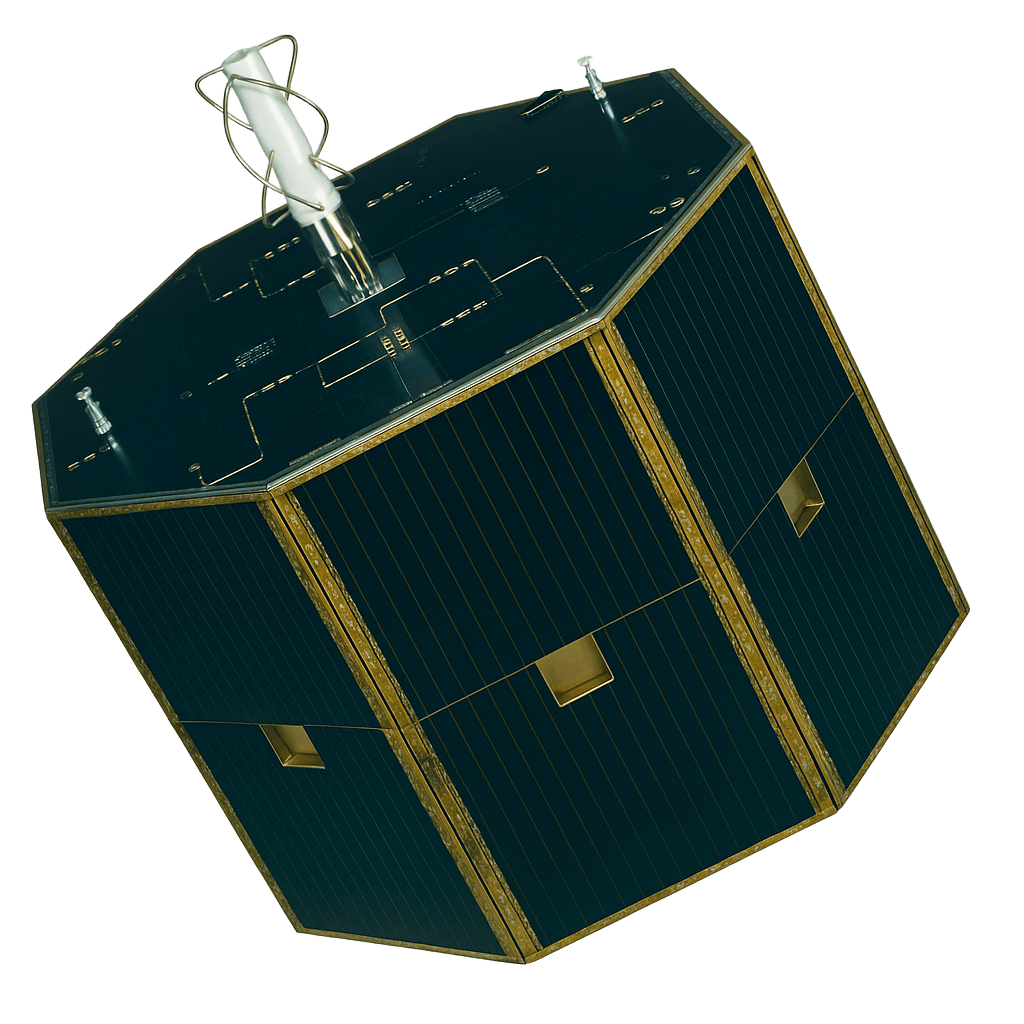
\includegraphics[width=0.7\linewidth]{assets/sat-SCD-1.png}
      \vspace{0.5em}
      \caption*{Satélite SCD-1}
      \small
      \begin{tabularx}{\linewidth}{>{\centering\arraybackslash}X >{\centering\arraybackslash}X}
        \toprule
        \textbf{Parâmetro} & \textbf{Valor} \\
        \midrule
        Massa & 115 kg \\
        Potência Elétrica & 110 W \\
        Vida útil & 4 anos \\
        Altitude média & $\approx$ 750 km \\
        Inclinação orbital & 25$^\circ$ \\
        Período orbital & 99,7 min \\
        \bottomrule
      \end{tabularx}
    \end{minipage}
    \hfill
    \begin{minipage}[t]{0.48\linewidth}
      \centering
      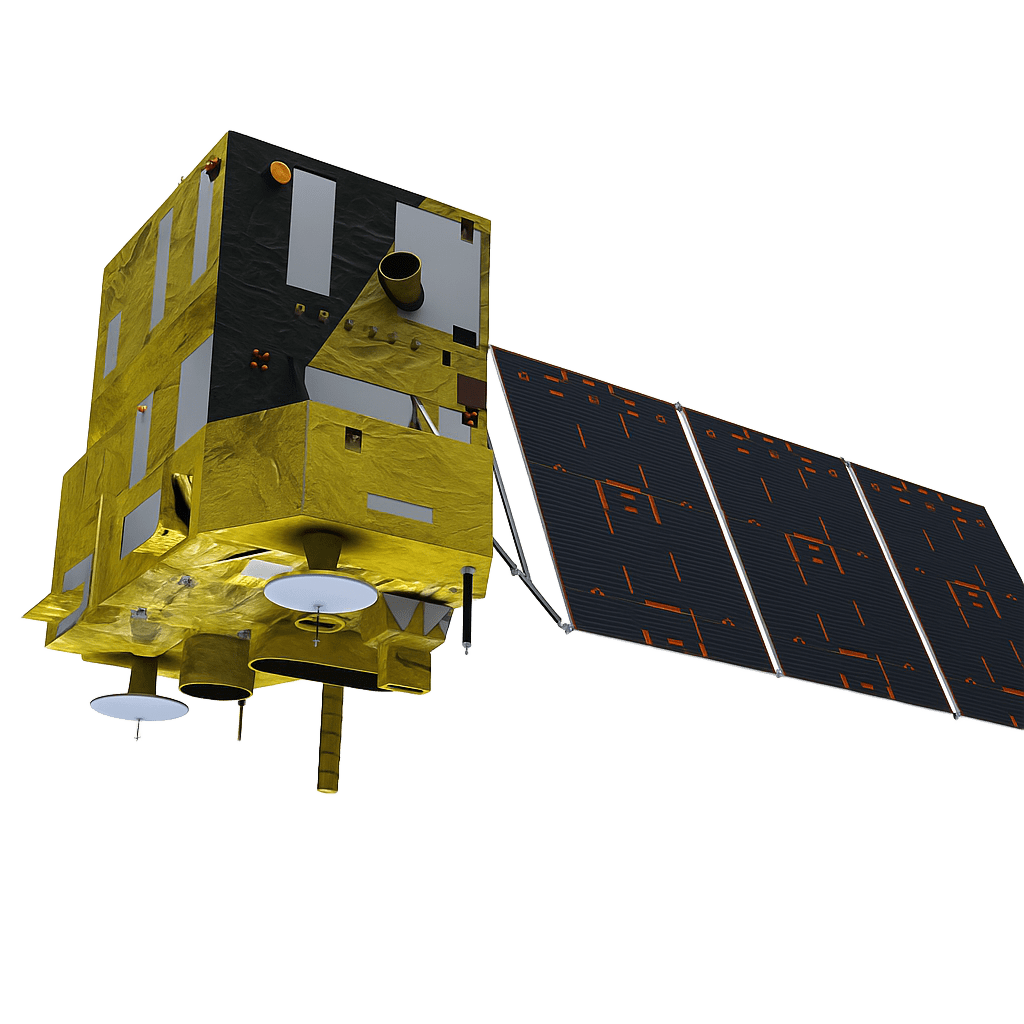
\includegraphics[width=0.7\linewidth]{assets/sat-CBERS-4.png}
      \vspace{0.5em}
      \caption*{Satélite CBERS-4}
      \small
      \begin{tabularx}{\linewidth}{>{\centering\arraybackslash}X >{\centering\arraybackslash}X}
        \toprule
        \textbf{Parâmetro} & \textbf{Valor} \\
        \midrule
        Massa & 1 980 kg \\
        Potência Elétrica & 2 300 W \\
        Vida útil & 3 anos \\
        Altitude média & $\approx$ 778 km \\
        Inclinação orbital & 98,54$^\circ$ \\
        Período orbital & 100,32 min \\
        \bottomrule
      \end{tabularx}
    \end{minipage}
    \vspace{0.5em}
    
\end{figure}

Esses satélites recebem sinais transmitidos pelas \gls{PCD} na faixa de frequência UHF (401,62 a 401,65 \gls{mhz}) e os retransmitem para as \gls{ETR} localizadas em solo, nas faixas de Banda-S (2267,5 \gls{mhz}). Como operam em órbitas baixas, esses satélites realizam aproximadamente 14 revoluções por dia sobre o território nacional, o que permite ampla cobertura espacial.

Apesar da ampla cobertura, a comunicação com satélites de órbita baixa apresenta um grande desafio técnico, sendo a necessidade de visada simultânea entre a \gls{PCD} transmissora e o satélite, o que limita a janela de transmissão e impõe restrições na coleta contínua de dados. Além disso, o movimento relativo entre a \gls{PCD} e o satélite provoca o chamado efeito Doppler, responsável por deslocamentos na frequência do sinal recebido, podendo atingir até ±79,4 \gls{khz}. Esse desvio precisa ser compensado para garantir a correta demodulação do sinal \cite{rae2005detector, rodrigues_demodulador_2018}.

A confiabilidade do enlace também é impactada por fatores como atenuação no espaço livre, ruídos térmicos, e variações atmosféricas. Para compensar esses fatores, são necessárias técnicas específicas de modulação, sincronização, codificação de dados e planejamento de enlace, de modo a garantir a confiabilidade das mensagens transmitidas.

\subsection{Constelação Catarina}

A Constelação Catarina é um projeto nacional baseado no uso de nanossatélites em órbita baixa, para atuar como um novo braço operacional do \gls{SBCDA}. A Constelação Catarina é composta por pequenos satélites integrados com \gls{SDR}, capazes de receber sinais transmitidos pelas \gls{PCD} no padrão \gls{ARGOS-II}, com planos futuros de migração para o padrão \gls{ARGOS-III} \cite{gomes_otimizacao_2024}.

Diferentemente dos satélites tradicionais, os nanosatélites da Constelação Catarina são projetados para realizar a decodificação e o armazenamento dos dados a bordo, o que permite superar a limitação de visada simultânea entre satélite e \gls{ETR}, ampliando a cobertura do sistema \cite{rodrigues_demodulador_2018}.

A arquitetura dos satélites que compõem a constelação é baseada na integração do transceptor \gls{AD9361} com uma \gls{FPGA} da \gls{Zynq-7000}, formando uma plataforma de \gls{SDR} altamente flexível \footnote{https://www.argos-system.org/wp-content/uploads/2023/01/ARTIC-Chipset-AnSem-Info-sheet.pdf}. Essa configuração permite a reconfiguração remota do hardware, o que é especialmente importante para futuras atualizações de protocolo ou migração para novos padrões de comunicação, como o \gls{PTT-A3}.


\section{EVOLUÇÃO DO SISTEMA ARGOS}\label{sec:quadros}

O \gls{ARGOS-II}, base do \gls{SBCDA} desde 1993, utiliza transmissores do tipo \gls{PTT-A2}, baseados em modulação analógica \gls{PM} com codificação Manchester. Essa versão se mostrou eficiente por muitos anos, mas suas limitações logo se tornaram evidentes, especialmente no que diz respeito à robustez frente a ruído, à largura de banda ocupada e à necessidade de visada simultânea entre \gls{PCD} e satélite para a \gls{ETR} \cite{cnes_services_and_message_formats_ed2_rev2_2006}.

A evolução desse sistema levou ao desenvolvimento do \gls{ARGOS-III}, que introduziu novas técnicas digitais de comunicação. Essa nova geração incorporou transmissores do tipo \gls{PTT-A3} e \gls{PTT-ZE}, os quais se destacam pela adoção de modulação \gls{QPSK}, codificação convolucional e embaralhamento de dados, resultando em maior confiabilidade na transmissão e maior eficiência espectral. Além disso, o \gls{ARGOS-III} permite o armazenamento e retransmissão de mensagens a bordo do satélite para a \gls{ETR} \cite{lima_parallel_2021, rodrigues_demodulador_2018}.

\section{ESPECIFICAÇÕES DO PADRÃO PTT-A3}

O transmissor do tipo \gls{PTT-A3} é um dos formatos definidos na terceira geração do sistema \gls{ARGOS}, projetado para oferecer maior robustez na transmissão e maior eficiência na utilização do espectro de frequência. 

A estrutura de um quadro \gls{PTT-A3} é composta por três campos principais, sendo eles: portadora pura, palavra de sincronismo (preâmbulo) e datagrama. Na \autoref{fig:estrutura_quadro}, a estrutura é apresentada de forma detalhada, considerando que a taxa de transmissão \gls{Rb} é de 400 \gls{bps} \textcite{cnes_services_and_message_formats_ed2_rev2_2006}.

\begin{figure}[H]
	\centering
	\caption{Estrutura do quadro de transmissão ARGOS-3}\label{fig:estrutura_quadro}
	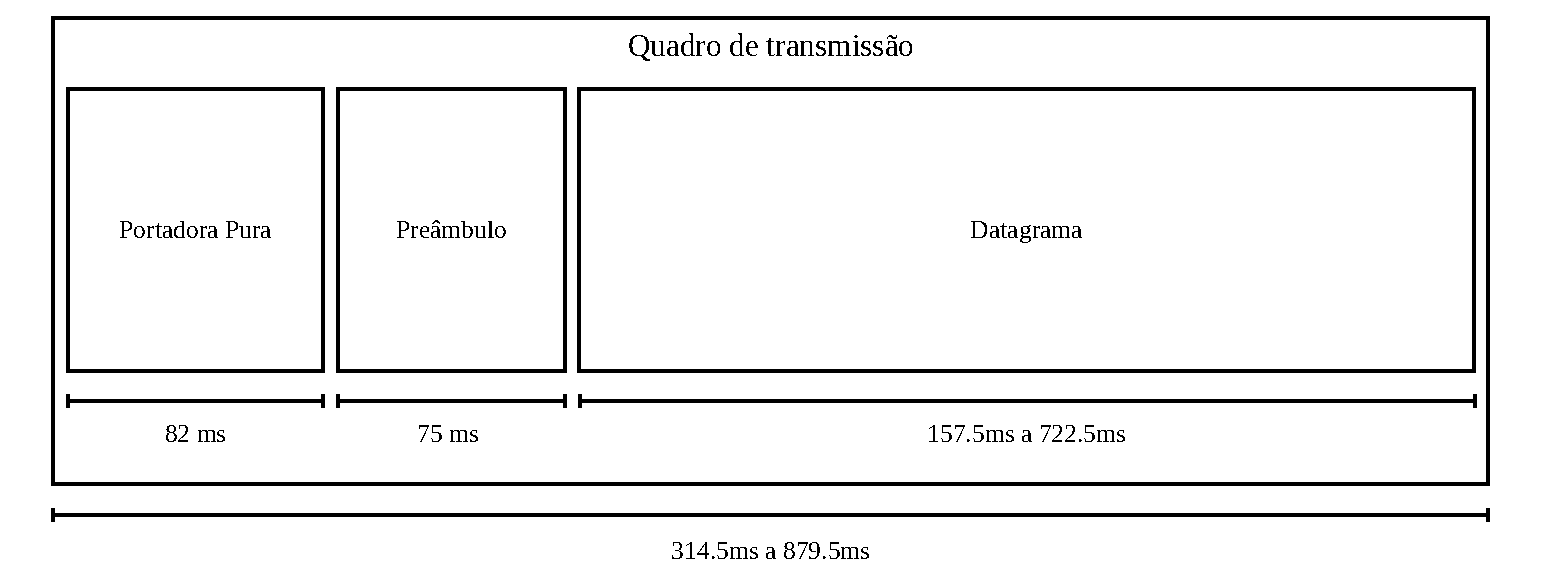
\includegraphics[width=\linewidth]{assets/quadro.pdf}
\end{figure}

\subsection{Portadora pura}

A sequência de transmissão do quadro inicia-se com a portadora contínua ou pura, com duração de 82 ± 2 ms. Durante essa etapa a portadora não transmite dados modulados e é utilizada pelo receptor apenas para realizar a detecção do sinal, bem como para facilitar o processo de sincronização de frequência e fase da portadora. 

A \autoref{fig:portadora_pura_freq} apresenta o sinal da portadora pura no espectro em comparação com o sinal modulado. Nota-se que quando apenas a portadora pura é transmitida, o espectro do sinal é concentrado em uma única frequência, sem componentes laterais. Já o sinal modulado apresenta componentes laterais que se estendem ao redor da frequência da portadora \gls{fc}, formando uma banda de uso do espectro mais ampla \cite{cnes_services_and_message_formats_ed2_rev2_2006}.


\begin{figure}[H]
	\centering
	\caption{Simulação de portadora pura no domínio da frequência}\label{fig:portadora_pura_freq}
	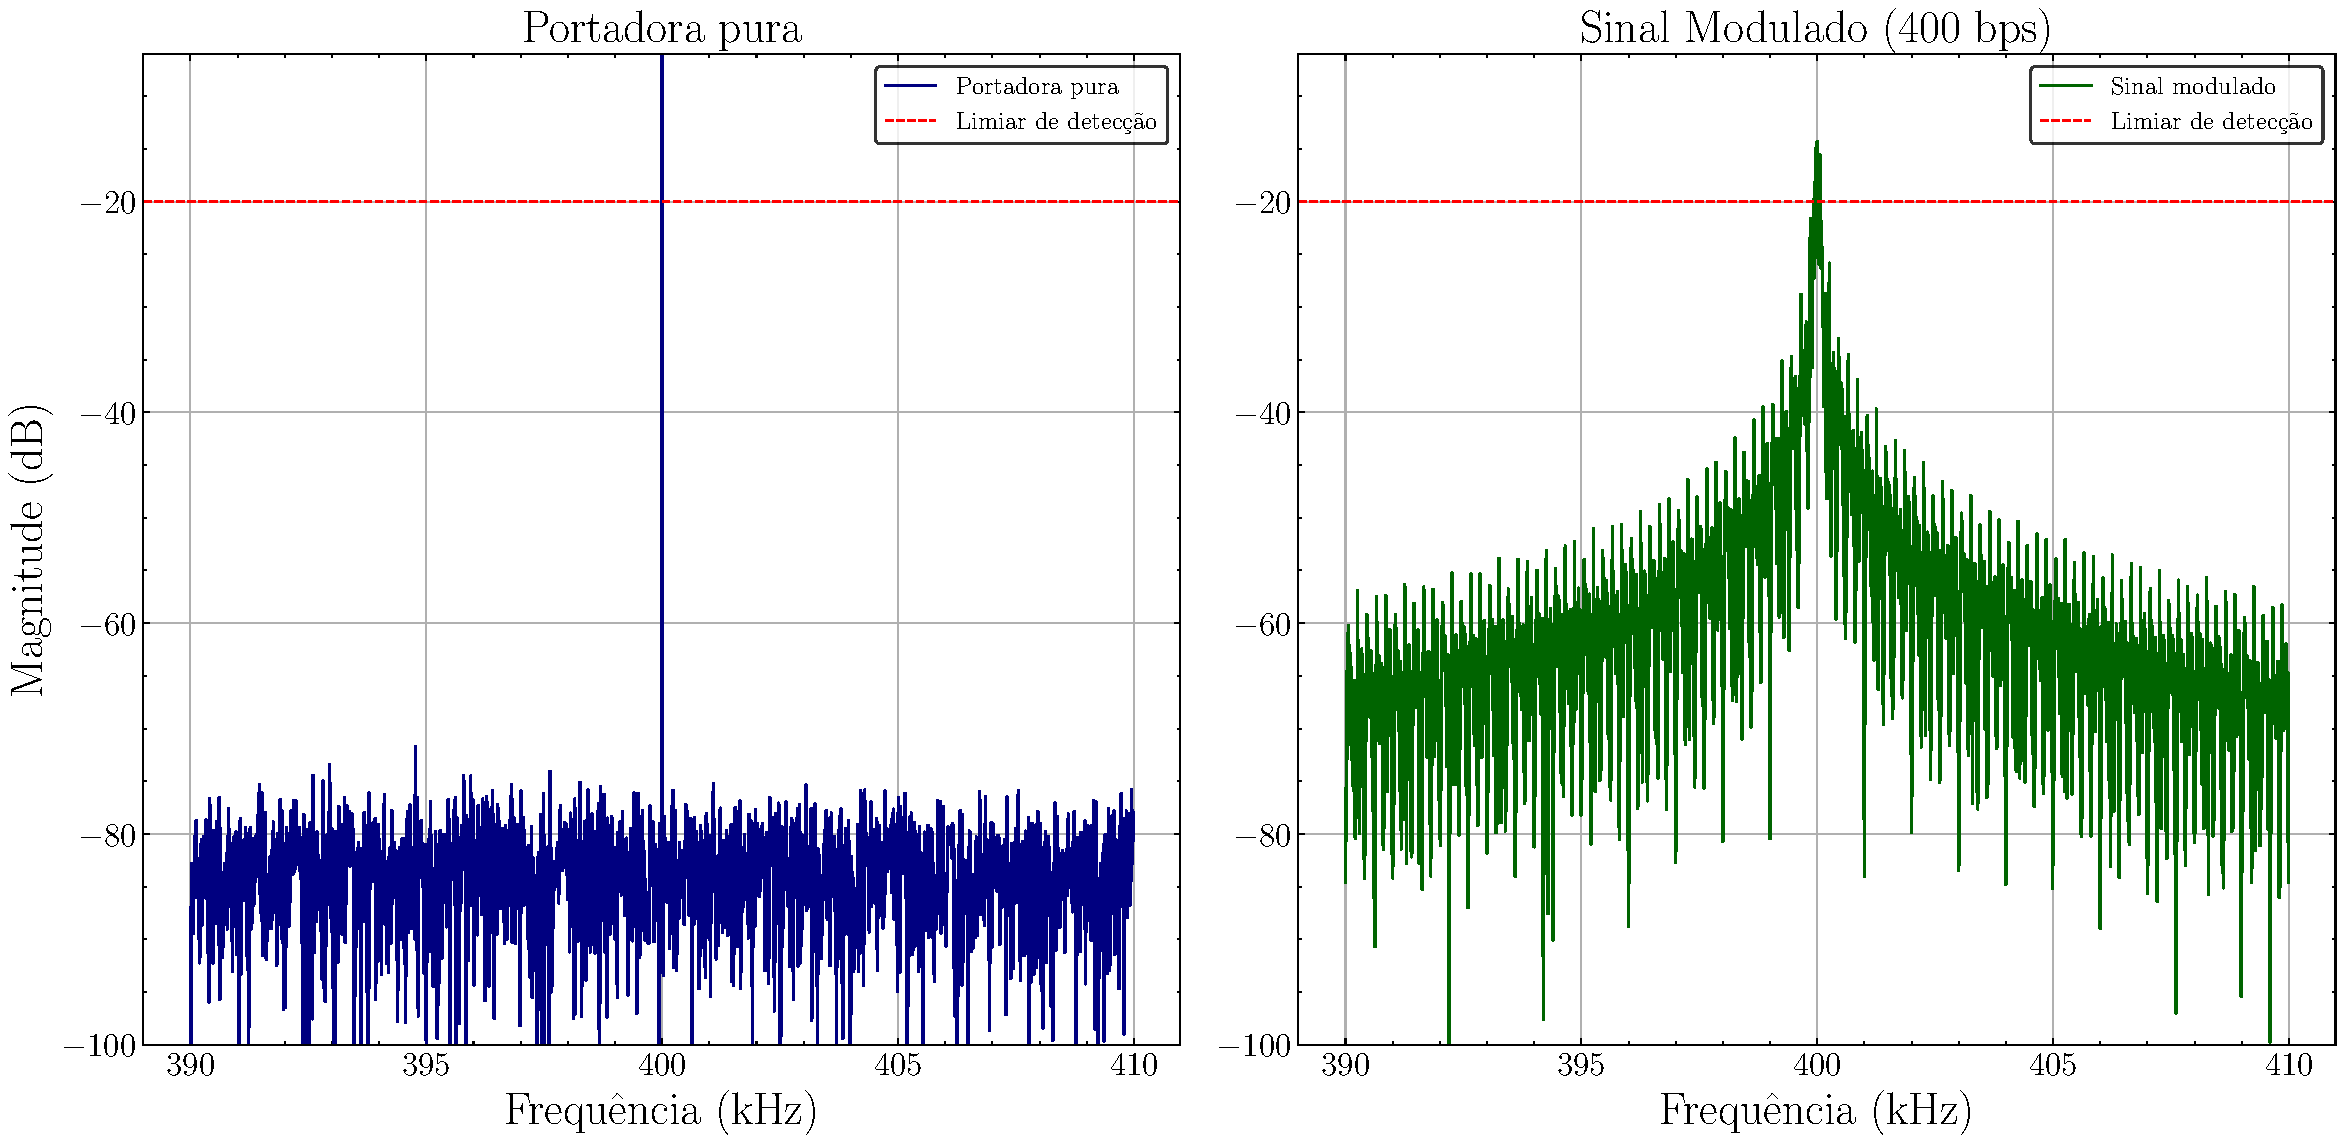
\includegraphics[width=\linewidth]{assets/plots/carrier_spectra.pdf}
    
\end{figure}

O processo de detecção do sinal realizado pelo receptor monitora a presença de sinal que ultrapassa um determinado limiar, dessa forma é fundamental que no receptor o sinal esteja o mais concentrado e com a maior \gls{SNR} possível no momento da detecção, para que a frequência da portadora, \gls{fc}, seja identificada corretamente \cite{cnes_services_and_message_formats_ed2_rev2_2006}.


\subsection{Palavra de sincronismo}

Logo após a portadora pura, é transmitida uma palavra de sincronismo de 30 bits (correspondente a 15 símbolos \gls{QPSK}), cuja função é auxiliar na identificação do início da mensagem codificada, possibilitando a sincronização para decisão. Essa sequência é conhecida e fixa entre transmissor e receptor, no caso do \gls{PTT-A3} sendo $S = \text{2BEEEEBF}_{16}$, o que permite alinhar corretamente a decisão e identificar o início do bloco de dados úteis. \cite{cnes_services_and_message_formats_ed2_rev2_2006}

A sequência \gls{Sn} é separada em dois vetores distintos, \gls{SIn} e \gls{SQn}, por meio de uma intercalação simples de seus bits. O processo de intercalação consiste em distribuir os bits de forma alternada entre os canais \gls{SIn} e \gls{SQn}, resultando em duas sequências de 15 bits cada, que serão transmitida como preâmbulo \cite{cnes_services_and_message_formats_ed2_rev2_2006}, usando a sequência padrão do \gls{ARGOS-III} podemos representar como

\vspace{-1em}
\begin{equation}
\begin{aligned}
    S_I[n] &= [S_0,\ S_2,\ S_4,\ \dots,\ S_{28}] &\mapsto&  S_I[n] = [1111,\ 1111,\ 1111,\ 111]     \\
    S_Q[n] &= [S_1,\ S_3,\ S_5,\ \dots,\ S_{29}] &\mapsto&  S_Q[n] = [0011,\ 0101,\ 0100,\ 111]
\end{aligned}
\label{eq:intercalacao}
\end{equation}

\noindent Importante destacar que esta palavra não é codificada convolucionalmente ou embaralhada, sendo adicionada ao início do vetor de bits de cada canal após esses blocos.  \cite{cnes_services_and_message_formats_ed2_rev2_2006}. 

\subsection{Datagrama}

Após o envio da palavra de sincronismo, inicia-se a transmissão dos dados modulados. Esses dados são organizados segundo a estrutura definida pelo datagrama do padrão \gls{ARGOS-III}, que contém os campos responsáveis pela identificação da plataforma, carga útil de dados e controle de finalização, conforme apresentado na \autoref{fig:datagrama} \cite{cnes_services_and_message_formats_ed2_rev2_2006}.

\begin{figure}[H]
	\centering
	\caption{Estrutura do datagrama ARGOS-3}\label{fig:datagrama}
	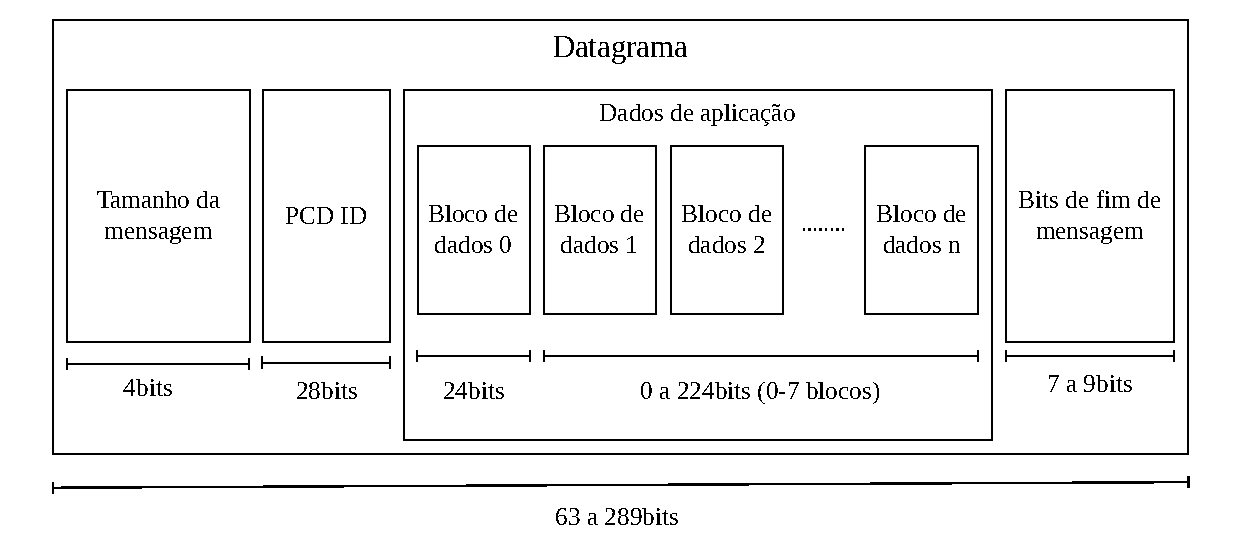
\includegraphics[width=\linewidth]{assets/datagrama.pdf}
    
\end{figure}

\section{ESTRUTURA DE UM DATAGRAMA ARGOS-3}

O datagrama transmitido no padrão \gls{ARGOS-III} possui uma estrutura bem definida, composta por campos de dados do usuário, que carregam as informações provenientes dos sensores da \gls{PCD}, e por campos de cabeçalho, responsáveis por identificar a estação transmissora e informar o comprimento total da mensagem. Esses campos incluem o identificador da PCD, o número de blocos de dados e um bit de paridade, que auxilia na verificação de integridade da informação. Essa organização permite que o sistema receptor interprete corretamente o conteúdo transmitido e associe os dados recebidos à plataforma correspondente.


\subsection{Dados de aplicação}

A primeira etapa na montagem do datagrama consiste na coleta dos dados de aplicação, isto é, os dados que efetivamente contêm informação dos sensores a serem transmitidos da \gls{PCD} para o satélite.

\subsubsection{Sensores}

Cada sensor presente nas \gls{PCD} gera um valor de oito bits correspondente à variável monitorada, possibilitando assim 256 ($2^8$) níveis de monitoramento para cada sensor. A PCD pode ser equipada com diferentes sensores, de acordo com o cenário de instalação e os parâmetros ambientais de interesse. 

Entre os sensores comumente utilizados, destacam-se os de direção do vento ($^{\circ}$), precipitação (mm), pressão atmosférica (mB), radiação solar acumulada (MJ/m2), temperatura do ar ($^{\circ}\text{C}$), umidade relativa ($\%$), e velocidade do vento (m/s). Por exemplo, os dados \footnote{http://sinda.crn.inpe.br/PCD/SITE/novo/site/historico/action.php} coletados da PCD 31855 são mostrados no \autoref{quadro:dados-meteorologicos}.


\begin{quadro}[H]
\caption{Dados meteorológicos da PCD 31855 (10/10/2007 - 11/10/2007)}\label{quadro:dados-meteorologicos}
\resizebox{\textwidth}{!}{%
\begin{tabular}{lccccccc}
    \toprule
    \textbf{DataHora} & \textbf{DirVento} & \textbf{Precip.} & \textbf{PressãoAtm} & \textbf{RadSolAcum} & \textbf{TempAr} & \textbf{UmidRel} & \textbf{VelVento} \\
    \midrule
    2007-11-10 21h & 0 & 0 & 945.5 & 2.3  & 30.8 & 25.6 & 0 \\
    2007-11-10 18h & 0 & 0 & 943.8 & 8.75 & 36.5 & 20.8 & 0 \\
    2007-11-10 15h & 0 & 0 & 947.3 & 9.72 & 33.6 & 28.8 & 0 \\
    2007-11-10 12h & 0 & 0 & 950.1 & 4.98 & 28.0 & 51.2 & 0 \\
    2007-11-10 09h & 0 & 0 & 949.3 & 0.17 & 20.9 & 60.8 & 0 \\
    2007-11-10 06h & 0 & 0 & 947.8 & 0.00 & 21.8 & 52.8 & 0 \\
    2007-11-10 03h & 0 & 0 & 948.0 & 0.00 & 23.5 & 40.0 & 0 \\
    2007-11-10 00h & 0 & 0 & 948.4 & 0.00 & 21.9 & 35.2 & 0 \\
    2007-11-09 21h & 0 & 0 & 946.1 & 0.48 & 30.8 & 20.8 & 0 \\
    2007-11-09 18h & 0 & 0 & 945.1 & 9.13 & 36.3 & 16.0 & 0 \\
    2007-11-09 15h & 0 & 0 & 948.4 & 10.13 & 34.5 & 22.4 & 0 \\
    2007-11-09 12h & 0 & 0 & 950.9 & 3.44 & 28.5 & 46.4 & 0 \\
    \bottomrule
\end{tabular}
}

\end{quadro}


\subsubsection{Blocos de dados}

Os dados dos sensores são agrupados em conjuntos denominados `blocos de dados` contendo quatro sensores por bloco, conforme ilustrado na \autoref{fig:sensores_blocos}. Assim, cada bloco de dados possui 32 bits ($4 \cdot 8$ bits), sendo o valor mínimo de um bloco de dados para montar um datagrama \gls{PTT-A3} (exceto o primeiro bloco que possui apenas 24 bits de comprimento). Para o caso específico em que a PCD irá transmitir apenas um bloco, ela poderá abrigar apenas três sensores. Caso haja mais de um bloco, o comprimento é dado por $24 + (\text{\gls{Nb} - 1}) \cdot 32$ bits \textcite{cnes_services_and_message_formats_ed2_rev2_2006}.

\begin{figure}[H]
	\centering
	\caption{Exemplo de agrupamento de sensores por bloco de dados}\label{fig:sensores_blocos}
	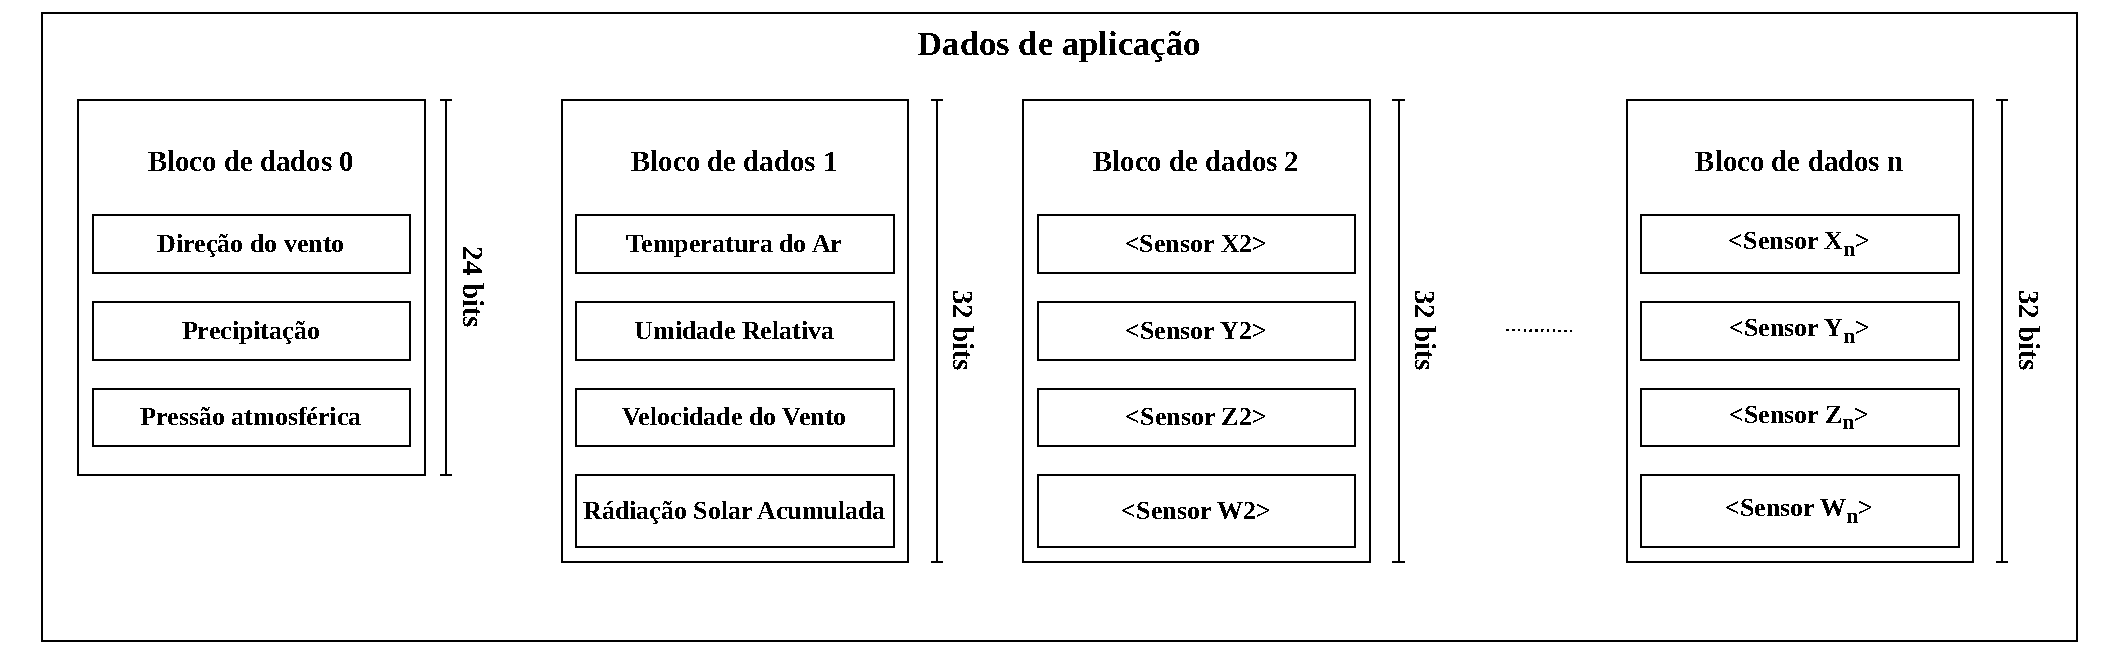
\includegraphics[width=\linewidth]{assets/dados_app.pdf}
\end{figure}


\subsection{Tamanho de mensagem}

O campo de tamanho de mensagem \gls{Tm} é utilizado para informar ao receptor quantos blocos de dados estão sendo transmitidos no datagrama, este campo é formado pelo número de blocos em formato binário \gls{Bm} e pelo bit de pariedade \gls{Pm} para fechar uma seção de 4 bits. Como cada bloco possui 32 bits (exceto o primeiro), é possivel determinar o comprimento total dos dados de aplicação de \gls{Bm} = ($N_b - 1)_{2}$. O número de blocos \gls{Nb}, pode variar de um a oito, resultando no compriemnto esperado de bits no receptor para cada caso, conforme o \autoref{quadro:comprimento-mensagem} abaixo. 

\begin{quadro}[H]
    \caption{Comprimento em bits para cada tamanho de mensagem ($T_m$)}
    \label{quadro:comprimento-mensagem}
    \small 
    \begin{tabularx}{\textwidth}{>{\centering\arraybackslash}X 
                                  >{\centering\arraybackslash}X 
                                  >{\centering\arraybackslash}X 
                                  >{\centering\arraybackslash}X 
                                  >{\centering\arraybackslash}X}
        \toprule
        \textbf{N° de Blocos} & \textbf{N° de Bits} & \textbf{$B_m$} & \textbf{$P_m$} & \textbf{$T_m$}\\
        \midrule
        1 & 24  & 000 & 0 & 0000\\
        2 & 56  & 001 & 1 & 0011\\
        3 & 88  & 010 & 0 & 0100\\
        4 & 120 & 011 & 1 & 0111\\
        5 & 152 & 100 & 0 & 1000\\
        6 & 184 & 101 & 1 & 1011\\
        7 & 216 & 110 & 0 & 1100\\
        8 & 248 & 111 & 1 & 1111\\
        \bottomrule
    \end{tabularx}
\end{quadro}

Conforme apresentado acima, para cada valor de \gls{Bm}, um valor de \gls{Pm} é calculado. O bit de paridade é calculado de forma a garantir que o número total de bits '1' na mensagem seja par, e é dado por

\vspace{-1em}
\begin{equation}
    P_m = 
    \begin{cases}
    1, & \text{se } \left[ \sum_{i=0}^{B_m} b_i = 0 \right]\mod 2  \\
    0, & \text{se } \left[ \sum_{i=0}^{B_m} b_i = 1 \right]\mod 2 
    \end{cases} \text{.}
\end{equation}

\noindent Ao final, o campo de tamanho de mensagem \gls{Tm} é formado pela concatenação do valor de \gls{Bm} e \gls{Pm}, resultando em um campo de 4 bits \textcite{cnes_services_and_message_formats_ed2_rev2_2006}. 


\subsection{Identificador da PCD}

O identificador da \gls{PCD}, \gls{pcdid}, é um campo de 28 bits presente na estrutura da mensagem do usuário no formato \gls{PTT-A3}. Ele é utilizado para identificar de forma única a \gls{PCD} que está transmitindo a mensagem, sendo essencial para o correto encaminhamento e associação dos dados recebidos no centro de controle do sistema \gls{ARGOS}, \textcite{cnes_services_and_message_formats_ed2_rev2_2006}. 

O \gls{pcdid} é formado por um número de 20 bits, \gls{ipcd}, seguido por oito bits \gls{rpcd} de redundância calculados através da soma (checksum) dos bits do identificador, conforme

\vspace{-1em}
\begin{equation}
R_{PCD} = \left( \sum_{i=0}^{19} I_{PCD} \cdot 2^i \right) \bmod 256 \text{ ,}
\end{equation}
\vspace{-0.2em}
\begin{equation}
    PCD_{ID} = I_{PCD} \oplus R_{PCD} \text{ .}
\end{equation}

\noindent   É importante destacar que a proteção contra erros nesse campo é assegurada de forma indireta pelo uso da codificação convolucional aplicada à mensagem como um todo, além da redundância oferecida pelo número de repetições da mensagem ao longo da passagem do satélite. 


\subsection{Bits de fim de mensagem}

Ao final do datagrama, são inseridos entre sete e nove bits '0' com a finalidade de limpar o registrador do codificador convolucional, dando o encerramento da sequência codificada. A quantidade de bits de fim de mensagem adicionados depende do comprimento total da mensagem do usuário, conforme apresentado na \autoref{quadro:bits-codificacao}. Apesar de não carregar dados úteis a nível de aplicação, esses bits são fundamentais para o correto funcionamento do processo de decodificação \cite{cnes_services_and_message_formats_ed2_rev2_2006}.

\begin{quadro}[H]
    \caption{Bits adicionados às mensagens do usuário antes da codificação}
    \label{quadro:bits-codificacao}
    \small 
    \begin{tabularx}{\textwidth}{>{\centering\arraybackslash}X 
                                  >{\centering\arraybackslash}X 
                                  >{\centering\arraybackslash}X 
                                  >{\centering\arraybackslash}X}
        \toprule
        \textbf{N° de Blocos} & \textbf{Bits Aplicação} & \textbf{Bits Datagrama} & \textbf{N° bits "0"} \\
        \midrule
        1 &  24 &  56 & 7 \\
        2 &  56 &  88 & 8 \\
        3 &  88 & 120 & 9 \\
        4 & 120 & 152 & 7 \\
        5 & 152 & 184 & 8 \\
        6 & 184 & 216 & 9 \\
        7 & 216 & 248 & 7 \\
        8 & 248 & 280 & 8 \\
        \bottomrule
    \end{tabularx}
    
\end{quadro}


\section{TRANSMISSOR PTT-A3}

Na \autoref{fig:diagrama_blocos_modulador} ilustra-se o diagrama de blocos do transmissor \gls{PTT-A3}. Cada bloco é responsável por uma etapa da transmissão, desde a montagem do datagrama até a modulação em banda passante e a transmissão do sinal \gls{st}.

\begin{figure}[H]
	\centering
	\caption{Diagrama de blocos do transmissor ARGOS-3}\label{fig:diagrama_blocos_modulador}
	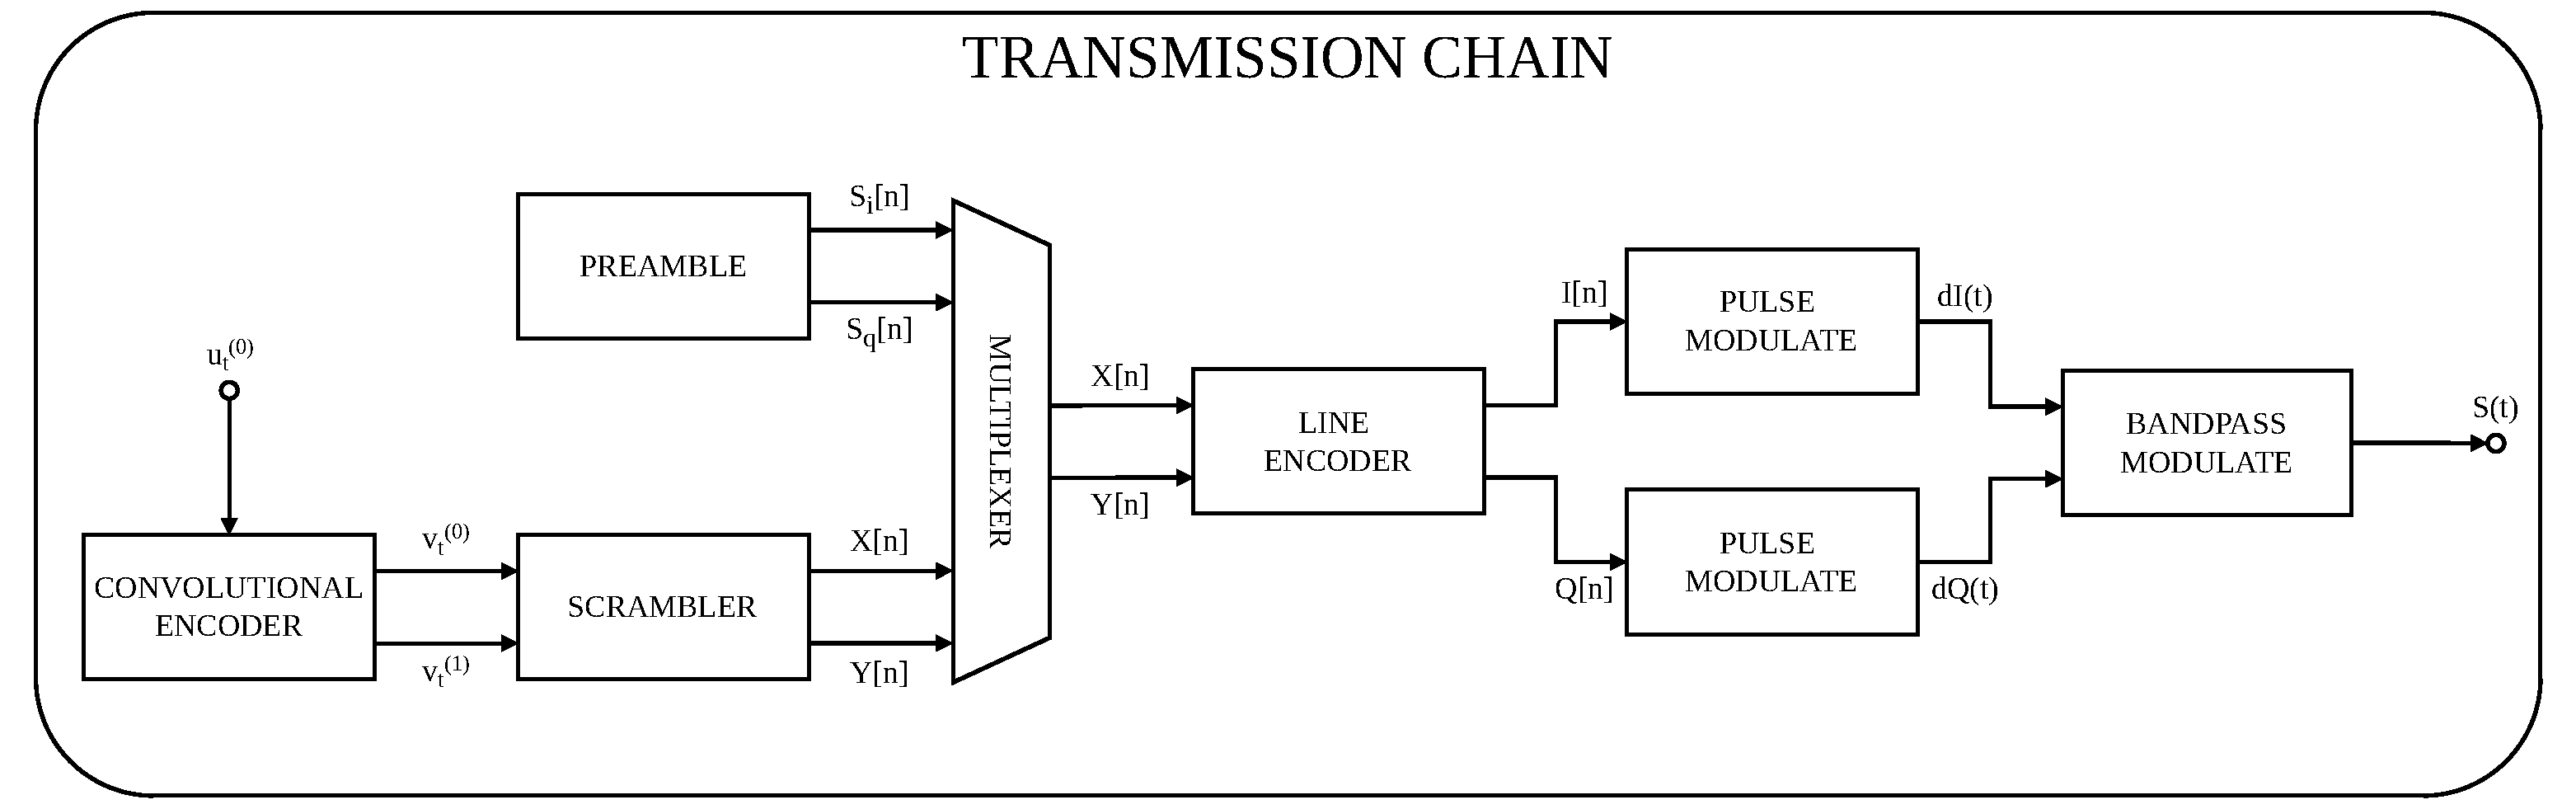
\includegraphics[width=\linewidth]{assets/blocos_modulador.pdf}
    
\end{figure}


\subsection{Codificador convolucional}

Antes da transmissão, os dados do datagrama precisam ser codificados, e esse processo é realizado através de um codificador convolucional. Essa técnica de codificação aplica uma operação lógica sobre uma janela deslizante de bits de entrada \gls{ut}, gerando uma sequência de saída com redundância controlada. Diferente da codificação por bloco, onde os dados são processados em blocos fixos, a codificação convolucional considera a sequência contínua de bits, combinando o bit atual com um número fixo de bits anteriores através de vetores geradores \cite{shu2011error}.

A taxa de codificação utilizada no padrão \gls{PTT-A3} é $R = \text{1/2}$, o que significa que para cada bit de dados de entrada \gls{ut}, são gerados dois bits de saída, um no canal \gls{cI} e outro no canal \gls{cQ}, aumentando a redundância e melhorando a capacidade do sistema de detectar e corrigir erros. Para a codificação convolucional, são utilizados vetores geradores \gls{G0} e \gls{G1}, de acordo com o padrão CCSDS 131.1-G-2 \cite{cnes_services_and_message_formats_ed2_rev2_2006}. A representação binária dos vetores geradores é dada por

\vspace{-1em}
\begin{equation}
    \begin{split}
        G_0 &= 121_{10} \quad \mapsto \quad G_0 = [1, 1, 1, 1, 0, 0, 1] \\
        G_1 &= 091_{10} \quad \mapsto \quad G_1 = [1, 0, 1, 1, 0, 1, 1] \text{.}
    \end{split}
\end{equation}

Os vetores geradores são utilizados para definir a estrutura do registrado do codificação convolucional aplicada à sequência de entrada \gls{ut}, resultando nas saídas \gls{vt0} e \gls{vt1}, que correspondem, respectivamente, aos canais \gls{cI} e \gls{cQ} utilizados posteriormente na modulação \gls{QPSK}. Essa operação pode ser representada por uma multiplicação vetorial entre uma janela deslizante de sete bits da entrada e a matriz formada pelos vetores geradores, conforme

\begin{equation}
\begin{aligned}
    \begin{bmatrix}
        v_t^{(0)} & v_t^{(1)}
    \end{bmatrix}
    &=
    \begin{bmatrix}
        u_{(t)} & u_{(t-1)} & u_{(t-2)} & u_{(t-3)} & u_{(t-4)} & u_{(t-5)} & u_{(t-6)}
    \end{bmatrix} \cdot \\
    &\quad
    \begin{bmatrix}
        1 & 1 & 1 & 1 & 0 & 0 & 1 \\
        1 & 0 & 1 & 1 & 0 & 1 & 1
    \end{bmatrix}^{T}
\end{aligned}
\label{eq:matriz_geradora}
\end{equation}

\noindent que pode ser representada de forma equivalente pelo diagrama de blocos apresentado na \autoref{fig:cod_convolucional} \cite{cnes_services_and_message_formats_ed2_rev2_2006}.

\begin{figure}[H]
	\centering
	\caption{Diagrama de blocos do codificador convolucional ARGOS-3}
	\label{fig:cod_convolucional}
	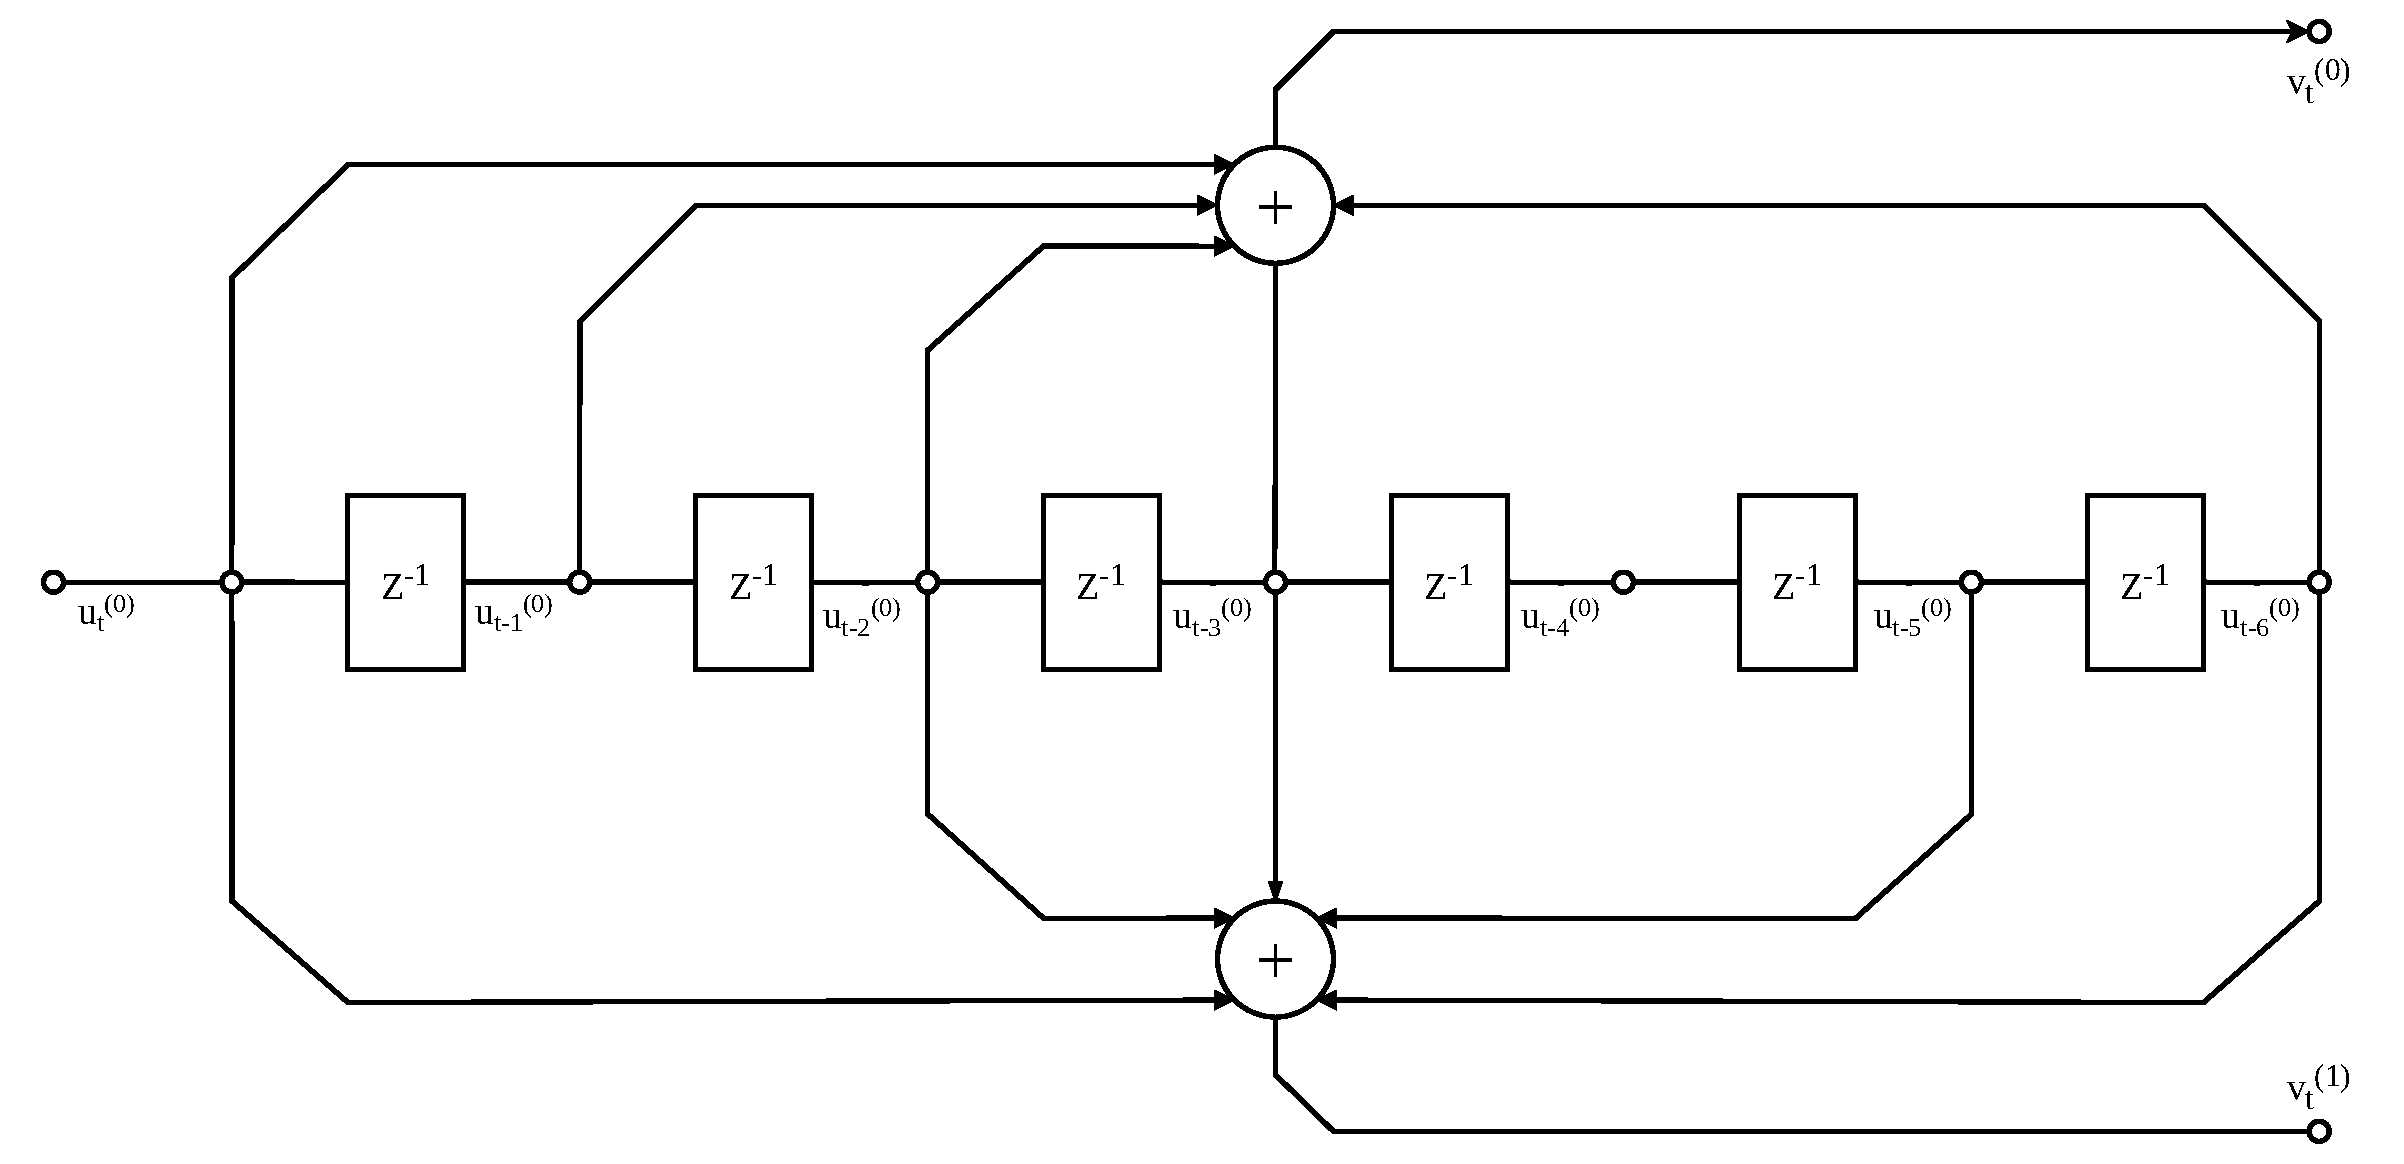
\includegraphics[width=\linewidth]{assets/cod_convolucional.pdf}
\end{figure}


\subsection{Embaralhador}

Após a codificação convolucional, os vetores de saída \gls{vt0} e \gls{vt1} são embaralhados para evitar padrões repetitivos, formando os vetores embaralhados \gls{Xn} e \gls{Yn}. O processo de embaralhamento é essencial para aumentar a robustez do sinal contra interferências e ruídos em rajada, pois os dados são espalhados ao longo da transmissão.

O embaralhador é utilizado para garantir que os dados sejam melhor distribuídos diminuindo a correlação entre os bits de forma a aumentar a aleatoriedade antes da modulação \gls{QPSK}, o que permite atingir uma melhor característica espectral. Esse processo pode ser representado pelo diagrama de blocos apresentado na \autoref{fig:embaralhador} \cite{cnes_services_and_message_formats_ed2_rev2_2006, rodrigues_demodulador_2018}.

\begin{figure}[H]
	\centering
	\caption{Embaralhador de dados para o ARGOS-3}\label{fig:embaralhador}
	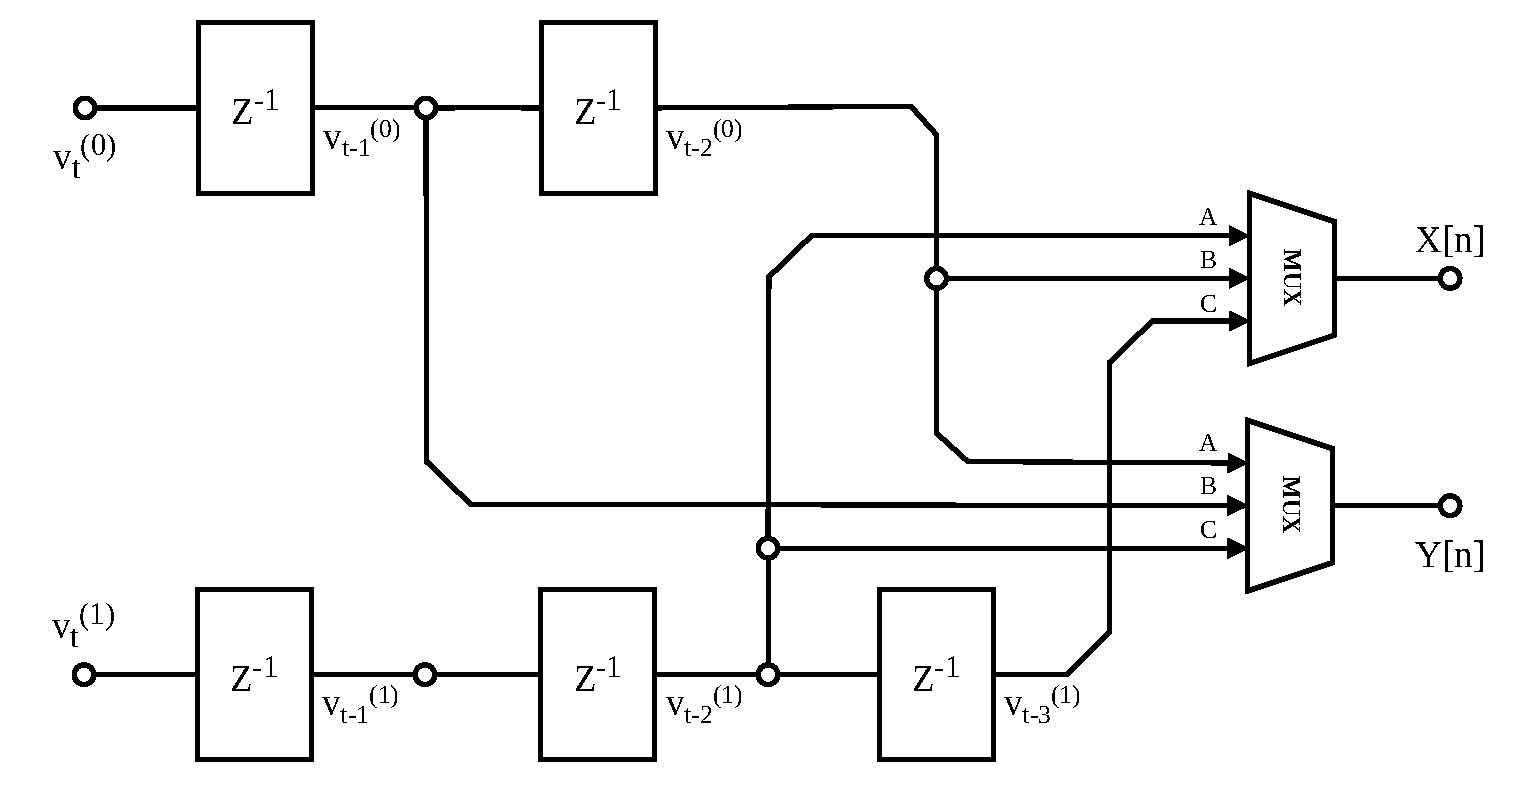
\includegraphics[width=\linewidth]{assets/scrambler.pdf}
    
\end{figure}


\subsection{Codificação de Linha}

Em seguida, os vetores de bits embaralhados \gls{Xn} e \gls{Yn}, já multiplexados com os vetores de preâmbulo \gls{SIn} e \gls{SQn},precisam ser convertidos em vetores de simbolos, para isso é aplicada uma codificação de linha. O vetor \gls{Xn} é codificado utilizando a técnica \gls{NRZ}, enquanto o vetor \gls{Yn} é codificado utilizando a técnica \gls{Manchester} \cite{cnes_services_and_message_formats_ed2_rev2_2006}.

A codificação \gls{NRZ} é realizada removendo a componente DC da sequência de entrada, ou seja, no vetor \gls{Xn} cada bit '1' é representado por '+1' e cada bit '0' é representado por '-1'. Esse processo pode ser descrito pela expressão

\begin{equation}
I[n] = 
\begin{cases}
+1, +1, & \text{se } X[n] = 1 \\
-1, -1, & \text{se } X[n] = 0 \text{ ,}
\end{cases}
\end{equation}

\noindent resultando em um vetor de saída \gls{In}, neste caso com o dobro do comprimento do vetor de entrada (para manter o mesmo comprimento do vetor \gls{Qn}). 

Para o vetor \gls{Yn}, é aplicada a codificação \gls{Manchester}, onde cada bit de entrada é representado por dois simbolos de saída, alternando entre '-1' e '+1'.  A codificação \gls{Manchester} é utilizada para garantir que haja transições de nível no sinal mesmo em sequências longas de bits iguais, essas transições refletem em mais trocas de simbolos na modulação \gls{QPSK}. Esse processo pode ser descrito pela expressão

\begin{equation}
Y[n] = 
\begin{cases}
+1,-1, & \text{se } Y[n] = 1 \\
-1,+1, & \text{se } Y[n] = 0 \text{ ,}
\end{cases}
\end{equation}

\noindent resultando assim em um vetor de saída \gls{Qn} codificado em Manchester.
\begin{figure}[H]
	\centering
	\caption{Codificação NRZ e Manchester dos vetores I e Q}\label{fig:codificacao_linha}
	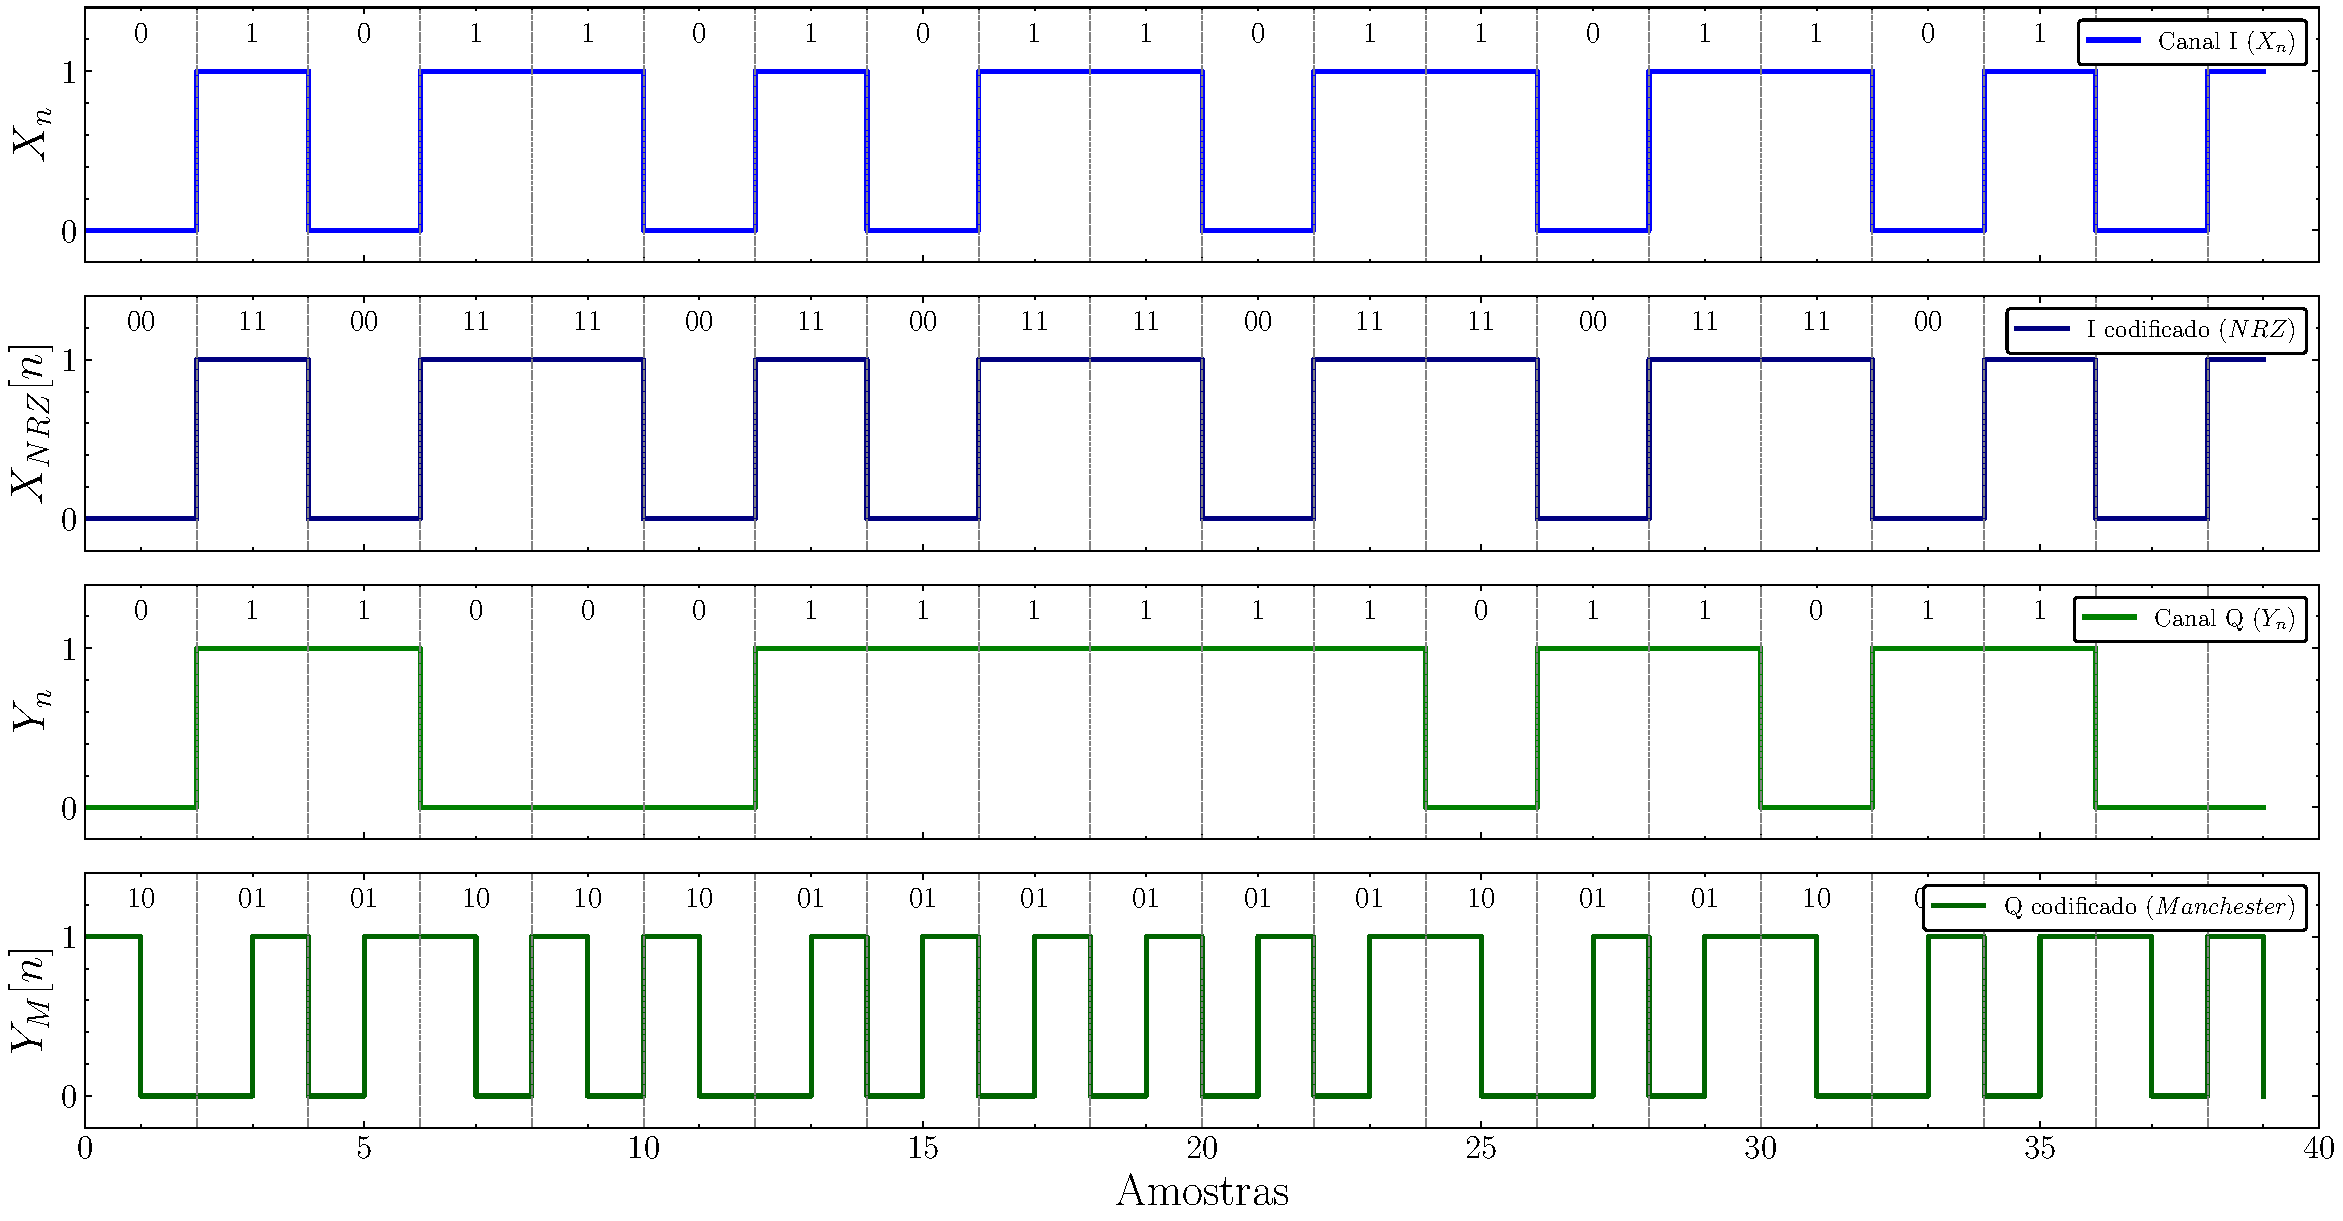
\includegraphics[width=\linewidth]{assets/codificacao_linha.pdf}
\end{figure}


\subsection{Modulação de Pulso}

Uma vez com os vetores de simbolo \gls{In} e \gls{Qn}, é aplicada a modulação de pulso, isto é, os vetores de simbolo são superamostrados, em função de \gls{fs} e filtrados para formar uma sequência contínua de símbolos ao longo de \gls{t}, onde cada bit de informação é transmitido durante um período de tempo $\text{ \gls{Tb}} = 1/ \text{\gls{Rb}}$ (tempo de bit), definido com base na taxa de bit \gls{Rb} \cite{cnes_services_and_message_formats_ed2_rev2_2006}.


Para aplicar a modulação de pulso e gerar os sinais analógicos \gls{dI} e \gls{dQ}, os vetores de simbolo são multiplicados com um pulso com resposta ao impulso \gls{gt}. A formatação é dada por 

\vspace{-1em}
\begin{equation}
    \begin{array}{c@{\quad\text{e}\quad}c}
        d_I'(t) = \sum_{n} I[n] \cdot g(t - nT_b) &
        d_Q'(t) = \sum_{n} Q[n] \cdot g(t - nT_b)
    \end{array} \text{ ,}
\end{equation}

\noindent onde é utilizado um pulso \gls{gt} do tipo (\gls{RRC}), definido por

\begin{equation}
    g(t) = \frac{(1-\alpha) \text{sinc}((1- \alpha) t / T_b) + \alpha(4/\pi) \cos(\pi(1 + \alpha)t/T_b) }{1 - (4\alpha )^2}
\end{equation}

\noindent onde \gls{alpha} é o fator de roll-off do pulso, que controla a largura de banda \gls{W} do sinal modulado. Quanto maior o \gls{alpha}, mais suave é a transição entre os símbolos, mas também maior é a largura de banda ocupada \cite{10555531840}.

A formatação dos vetores \gls{In} e \gls{Qn} é ilustrada na \autoref{fig:pulso_rrc_e_sinais_iq}, onde a resposta ao impulso \gls{gt} é apresentada em conjunto com os sinais \gls{dI} e \gls{dQ}. 

\begin{figure}[H]
	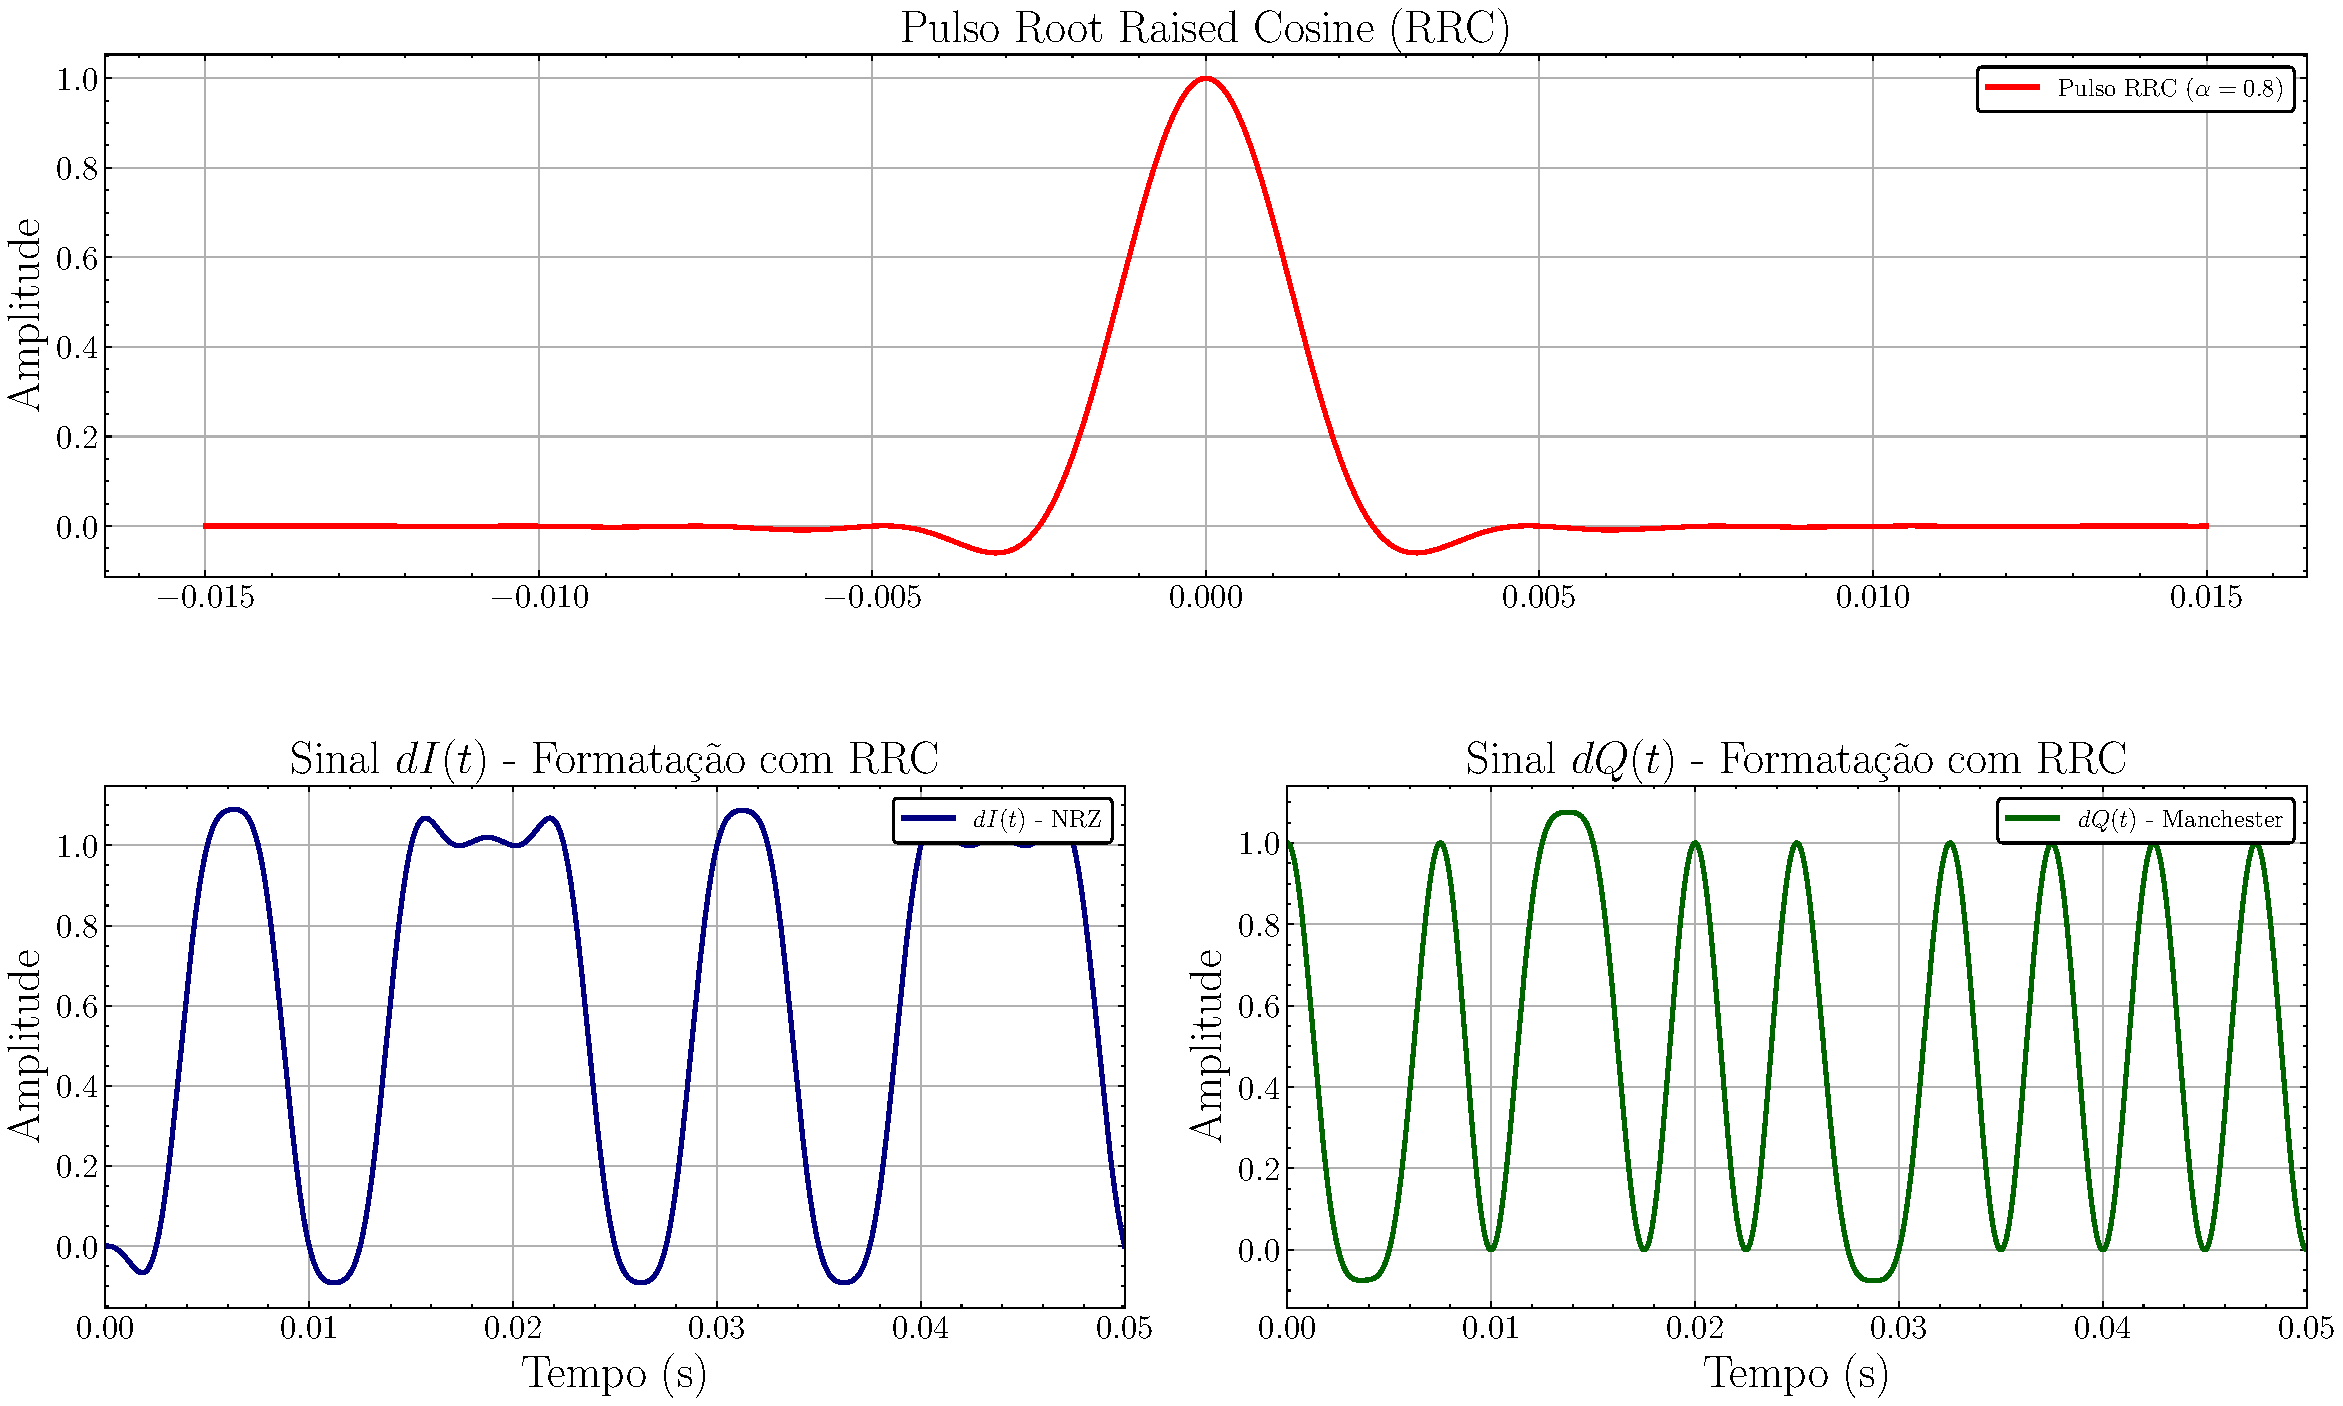
\includegraphics[width=\linewidth]{assets/pulso_rrc_e_sinais_iq.pdf}
	\caption{Formatação dos pares IQ}\label{fig:pulso_rrc_e_sinais_iq}
\end{figure}



\subsection{Modulação em banda passante} 

Uma vez com os pares de sinal \gls{dI} e \gls{dQ} correspondentes a cada canal, pode-se realizar a modulação em banda passante para transmissão do sinal \gls{st}. Na \autoref{fig:modulador_qpsk} é ilustrado o diagrama de blocos do modulador \gls{QPSK} \cite{cnes_services_and_message_formats_ed2_rev2_2006}.

\begin{figure}[H]
	\centering
	\caption{Modulador QPSK}\label{fig:modulador_qpsk}
	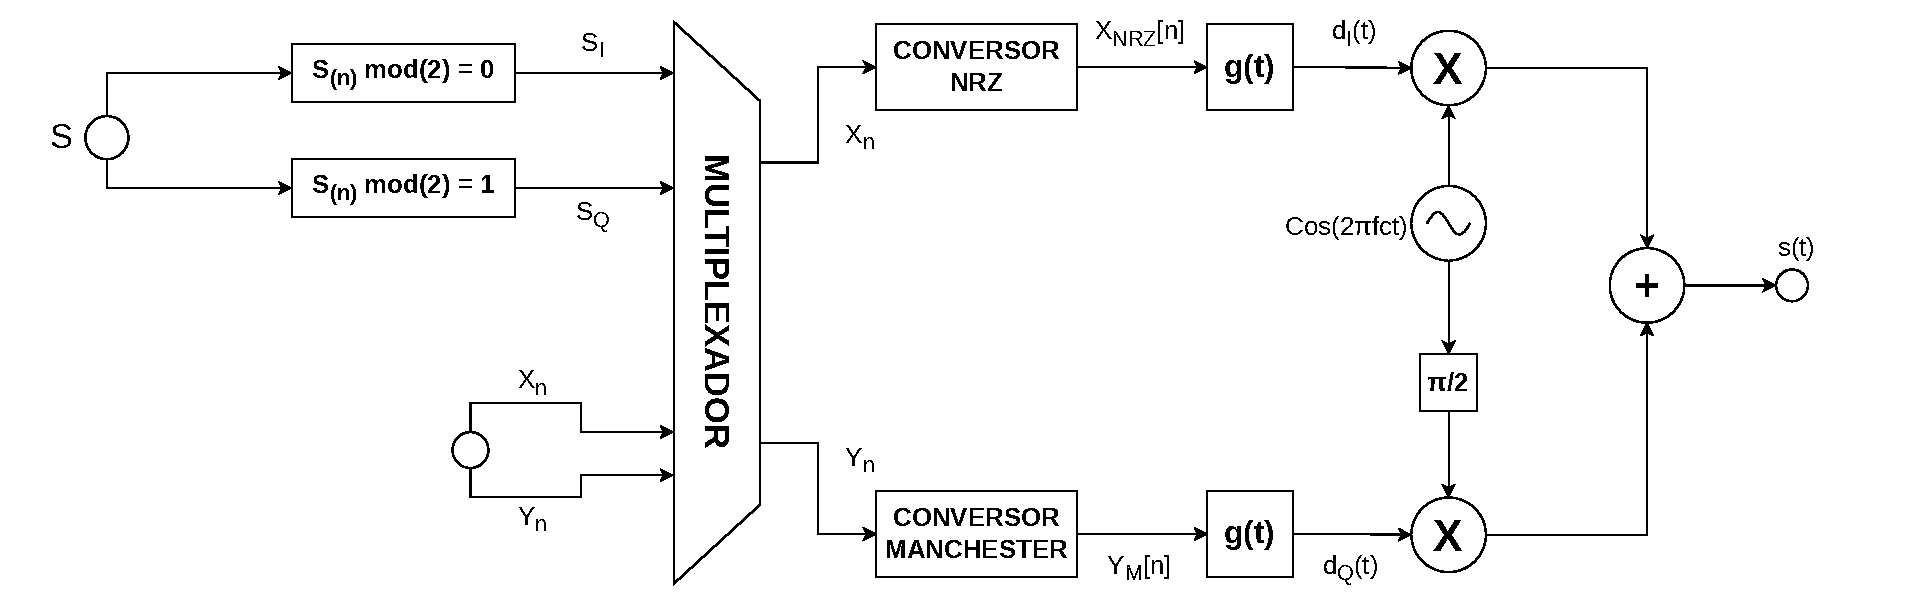
\includegraphics[width=\linewidth]{assets/modulador.pdf}
    
\end{figure}

No processo de modulação QPSK, o sinal em fase \gls{dI} é multiplicado por uma componente cossenoidal em frequência \gls{fc} e o sinal em quadratura \gls{dQ} é multiplicado por uma componente senoidal em \gls{fc}, seguindo a expressão

\vspace{-0.8em}
\begin{equation}
    s(t) = A d_I'(t) \cos(2\pi f_c t + \phi_0) - Ad_Q'(t) \sin(2\pi f_c t + \phi_0) \text{ ,}
\end{equation}

\noindent onde \gls{A} é a amplitude do sinal modulado, \gls{fc} é a frequência da portadora, em torno de $401,625$ \gls{mhz} e \gls{phi0} é o desvio de fase inicial do sinal, que é considerado como zero ($\phi_0 = 0$).

A \autoref{fig:qpsk_sinais_e_constelacao} ilustra o processo de modulação IQ, mostrando os sinais \gls{dI} e \gls{dQ} e a constelação resultante dos símbolos \gls{QPSK} no plano complexo, onde cada ponto representa um símbolo modulado.

\begin{figure}[H]
	\centering
	\caption{Modulação IQ}\label{fig:qpsk_sinais_e_constelacao}
	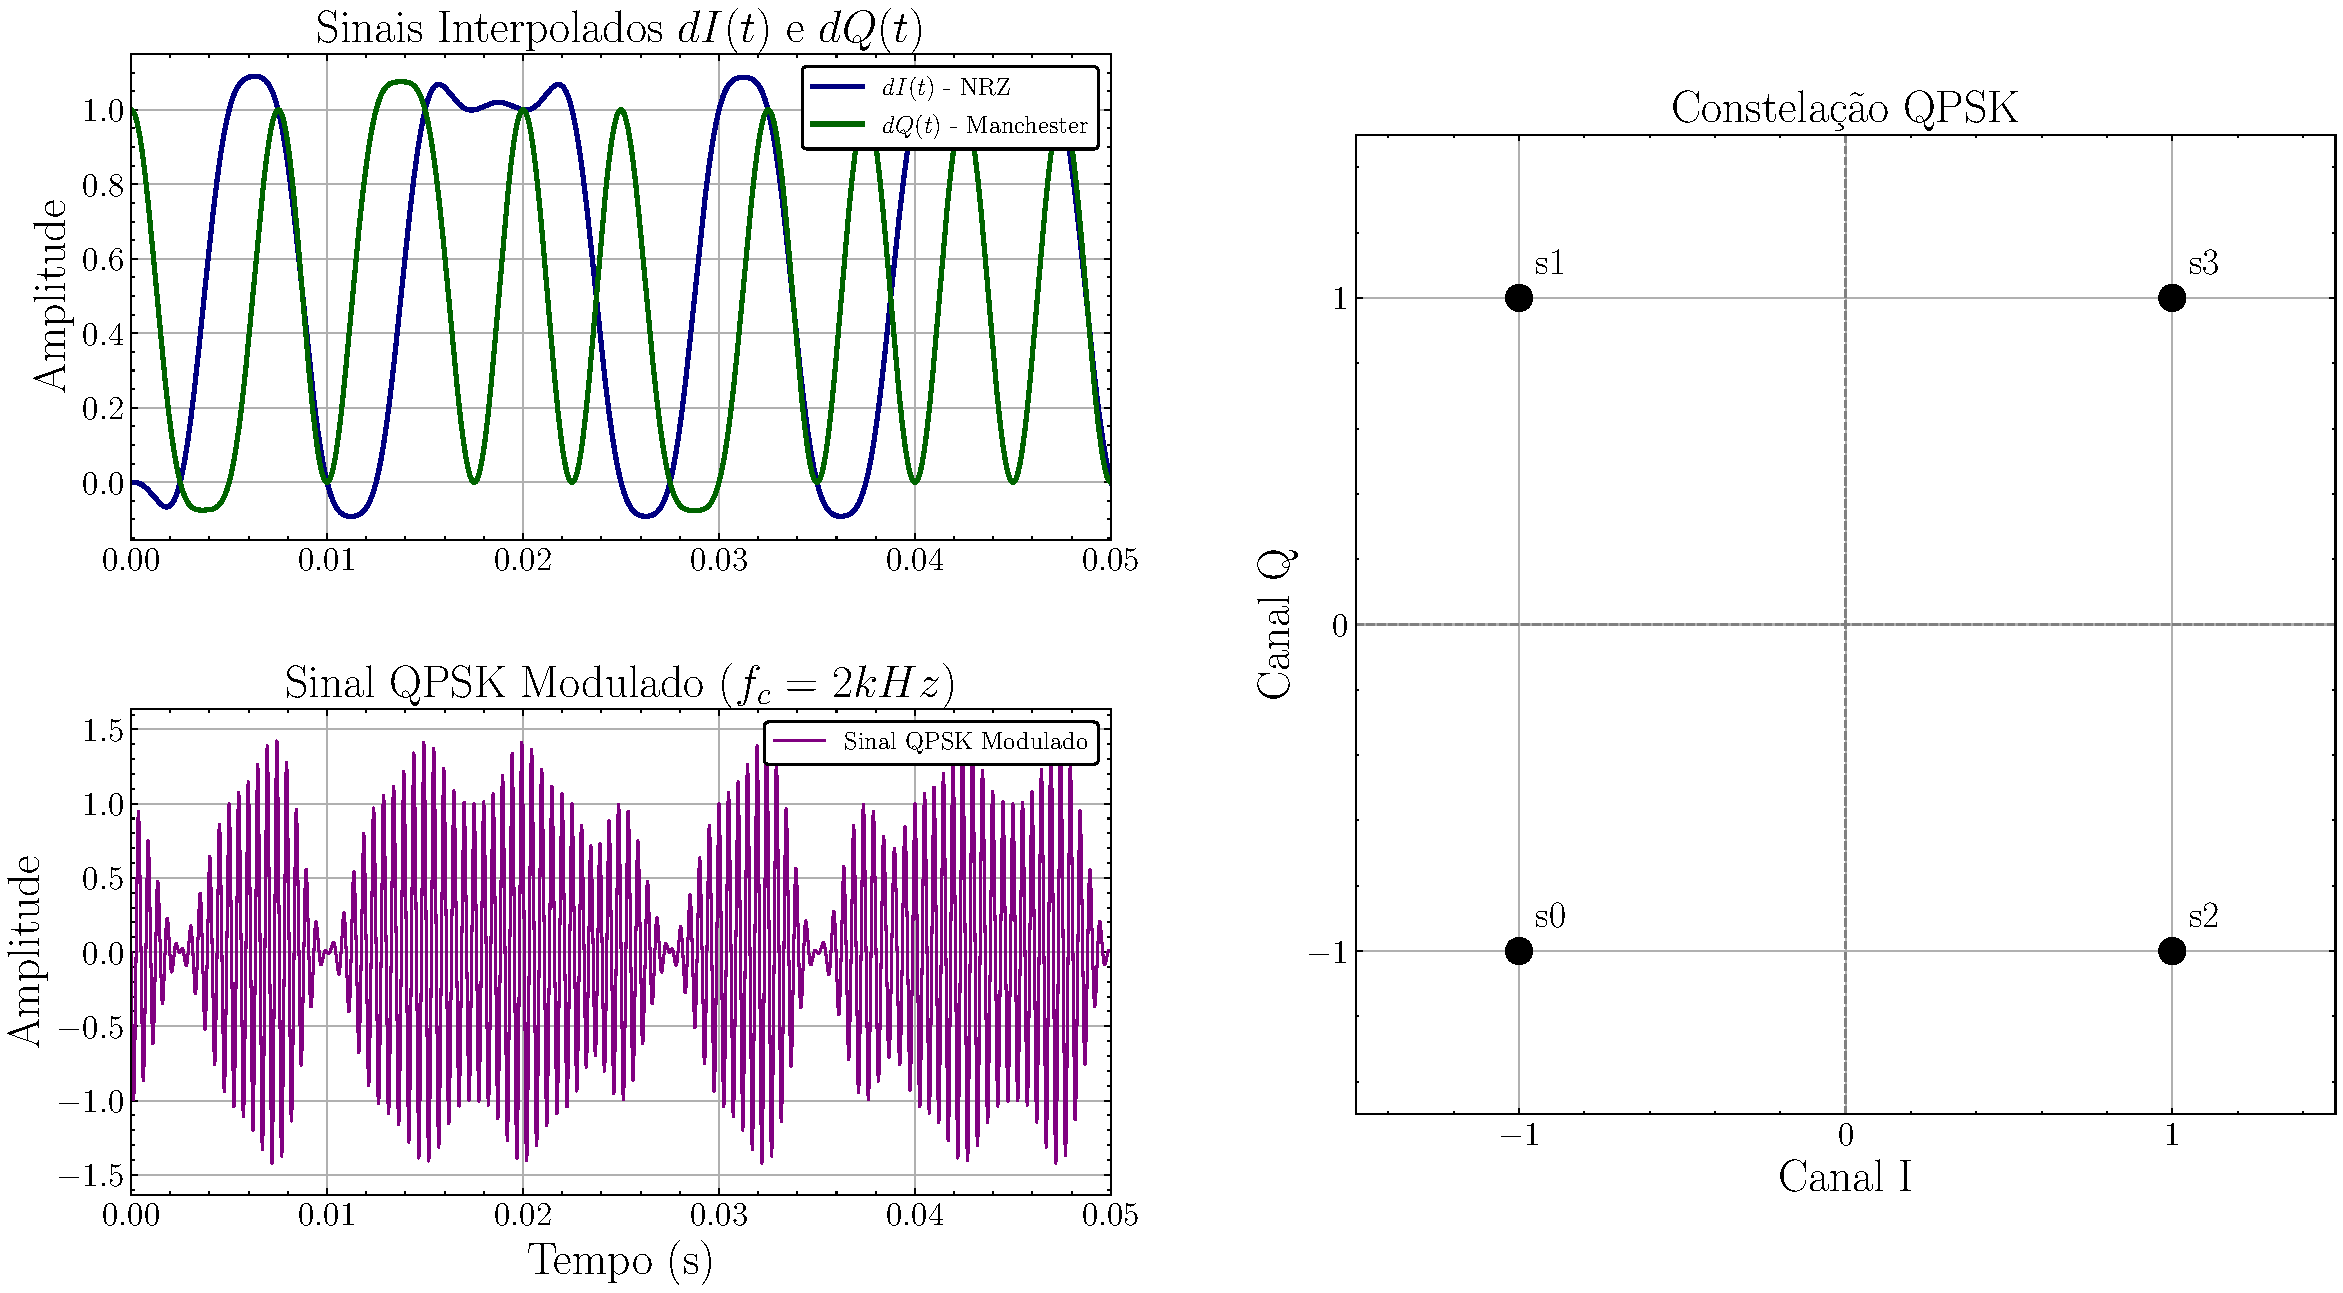
\includegraphics[width=\linewidth]{assets/qpsk_sinais_e_constelacao.pdf}
\end{figure}

A constelação \gls{QPSK} na \autoref{fig:qpsk_sinais_e_constelacao} é composta por quatro pontos, cada qual representando um símbolo distinto. Os símbolos são mapeados de acordo com os pares de bits \gls{dI} e \gls{dQ}. Após a transmissão, o sinal \gls{st} é somado a um vetor de ruído \gls{rt} para simular as condições reais no momento da recepção.

\section{RECEPTOR PTT-A3}

Como a transmissão dos dados das \gls{PCD} não segue uma estrutura de canais discretos, ou seja, cada \gls{PCD} seleciona uma frequência \gls{fn} dentro da faixa de $401,62$ a $401,65MHz$ e realiza a transmissão. Dessa forma, o receptor no satélite necessita de um mecanismo de detecção de portadora para avaliar as candidatas de \gls{fc}, podendo assim demodular o sinal.

\begin{figure}[H]
	\centering
	\caption{Diagrama de blocos do demodulador}\label{fig:diagrama_blocos_demodulador}
	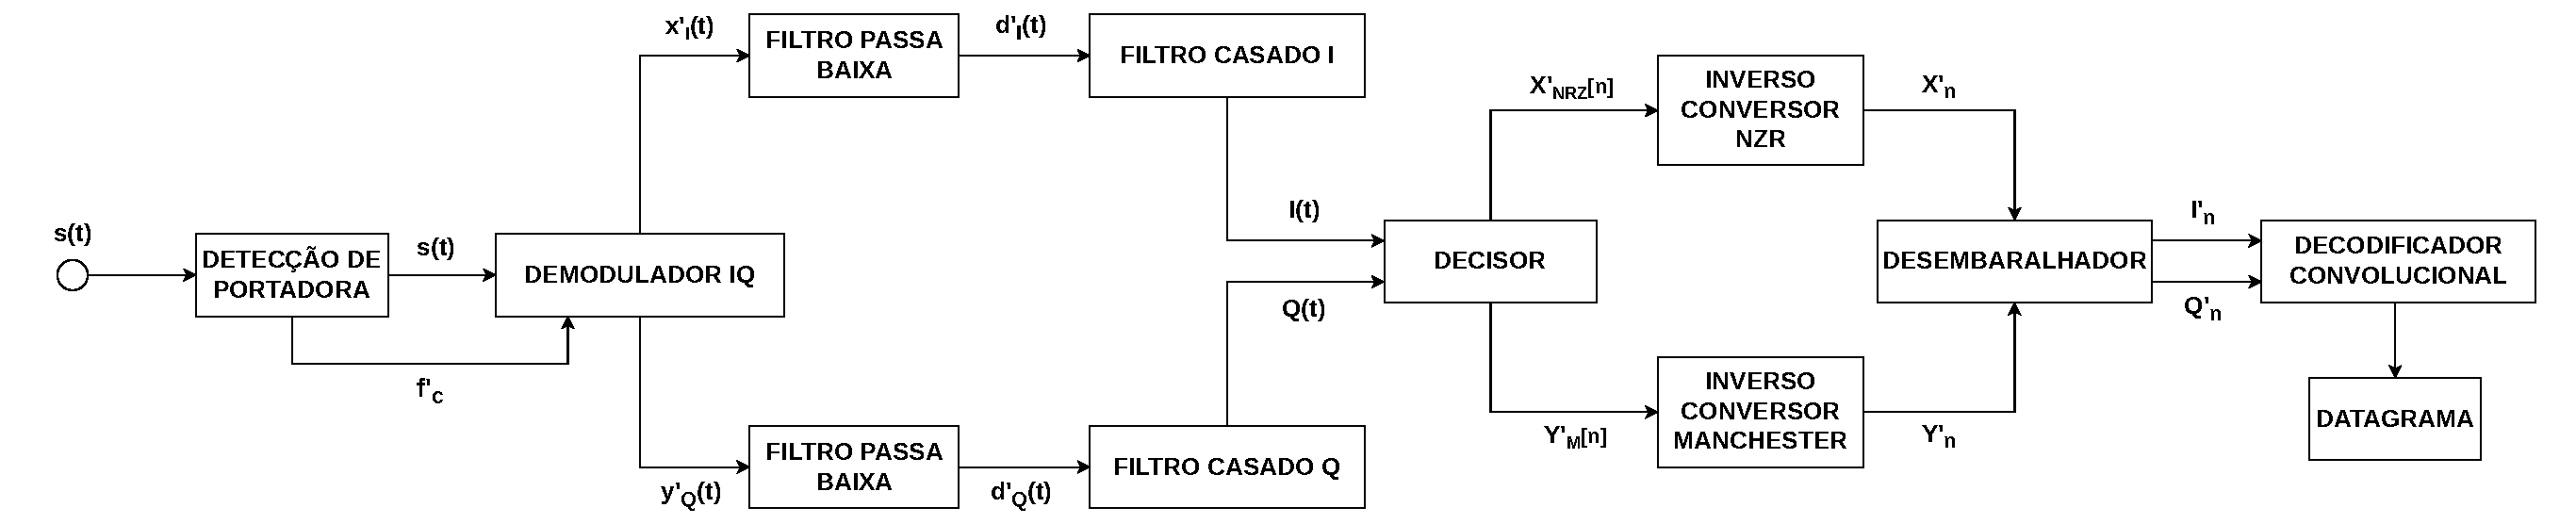
\includegraphics[width=\linewidth]{assets/blocos_demodulador.pdf}
\end{figure}


\subsection{Detecção de portadora}

Para realizar a detecção da portadora, o sinal recebido acrescido de ruído deve ser inicialmente amostrado e dividido em segmentos discretos \gls{xn} no tempo. O satélite \gls{ARGOS} realiza a decisão do sinal a cada $10 \text{ms}$, esse processo é definido por 

\vspace{-0.4em}
\begin{equation}
    x_n[m] = s(mT_n) \text{ ,}
\end{equation}

\noindent onde \gls{xn} representa o segmento de sinal, \gls{st} é o sinal recebido, \gls{m} é o índice de amostra do segmento de tempo e \gls{Tn} é o tempo de amostragem, definido como $T_n = f_s * 10 \text{ms}$, onde \gls{fs} é a frequência de amostragem do sistema. 


Em seguida, aplica-se a \gls{FFT} no vetor \gls{xn}, obtendo-se o espectro de frequência do sinal amostrado \gls{xnk}, conforme a expressão 

\vspace{-0.4em}
\begin{equation}
    X_n[k] = \sum_{m=0}^{N-1} x_n[m]\, e^{-j2\pi km/N} \text{ .}
\end{equation}

A partir da amostras de \gls{xnk}, se calcula a potência em cada componente de frequência, para obter os valores \gls{Pnk}, conforme

\vspace{-0.4em}
\begin{equation}
    P_n[k] = |X_n[k]|^2 \text{ .}
\end{equation}

Em seguida, para cada índice \gls{k} do espectro calculado, é feita uma comparação com um limiar pré-definido \gls{Pt}, conforme foi apresentado anteriormente na \autoref{fig:portadora_pura_freq}. Caso a potência \gls{Pnk} seja maior que \gls{Pt}, a frequência é registrada pois existe a possibilidade de que uma portadora \gls{fn} esteja presente naquela frequência. 

Por fim, no proximo segmento, $X_{n+1}[k]$, o sistema verifica se a frequência registrada no segmento anterior persiste, ou seja, se a potência de $k$ também é maior que o limiar \gls{Pt}, caso positivo, o sistema considera que a frequência \gls{fn} é a portadora \gls{fc} do sinal recebido e instância a cadeia de recepção passando \gls{fc} como parâmetro.



\subsection{Demodulador Banda Passante}

Para realizar a demodulação do sinal \gls{st} recebido retornando as componentes \gls{dXt} e \gls{dYt} em banda base, o sinal \gls{st} é multiplicado por duas portadoras ortogonais, \gls{xi} para demodular o canal \gls{cI} e \gls{yq} para demodular o canal \gls{cQ}. Assumindo sincronismo perfeito, o processo de demodulação para o canal \gls{cI} pode ser expresso como

\vspace{-1.2em}
\begin{equation}
d_X'(t) = s(t) \cdot x_I(t) = \left[A \cdot d_I'(t) \cos(2\pi f_c t ) - A \cdot d_Q'(t) \sin(2\pi f_c t )\right] \cdot 2\cos(2\pi f_c t )
\end{equation}
\vspace{-0.8em}
\begin{equation}
    d_X'(t) =
    \underbrace{A \cdot d_I'(t)}_{\text{Banda base}} + 
    \underbrace{\left[
        A \cdot d_I'(t) \cos(4\pi f_c t ) 
        - A \cdot d_Q'(t) \sin(4\pi f_c t )
    \right]}_{\text{Dobro da frequência $f_c$}} \text{ ,}
\end{equation}

\noindent onde \gls{dI} é o sinal banda base. O mesmo processo é realizado para o canal \gls{cQ}, que isola o sinal em quadratura \gls{dQ} da seguinte forma

\vspace{-1.2em}
\begin{equation}
d_Y'(t) = s(t) \cdot y_Q(t) = \left[A \cdot d_I'(t) \cos(2\pi f_c t ) - A \cdot d_Q'(t) \sin(2\pi f_c t )\right] \cdot 2\sin(2\pi f_c t )
\end{equation}
\vspace{-0.8em}
\begin{equation}
    d_Y'(t) =  
    \underbrace{A \cdot d_Q'(t)}_{\text{Banda base}} + 
    \underbrace{\left[
        A \cdot d_Q'(t) \cos(4\pi f_c t ) 
        + A \cdot d_I'(t) \sin(4\pi f_c t )
    \right]}_{\text{Dobro da frequência $f_c$}} \text{ .}
\end{equation}

A \autoref{fig:fft_produtos_com_portadoras} ilustra o processo de demodulação dos canais \gls{cI} e \gls{cQ}, onde os sinais multiplicados por \gls{xi} e \gls{yq} são apresentados no espectro, mostrando a presença dos sinais em banda base e as componentes de alta frequência resultantes da multiplicação com as portadoras (considerando um $f_c = 2 \text{\gls{khz}}$). \cite{cnes_services_and_message_formats_ed2_rev2_2006}

\begin{figure}[H]
	\centering
	\caption{Demodulação dos canais I e Q}\label{fig:fft_produtos_com_portadoras}
	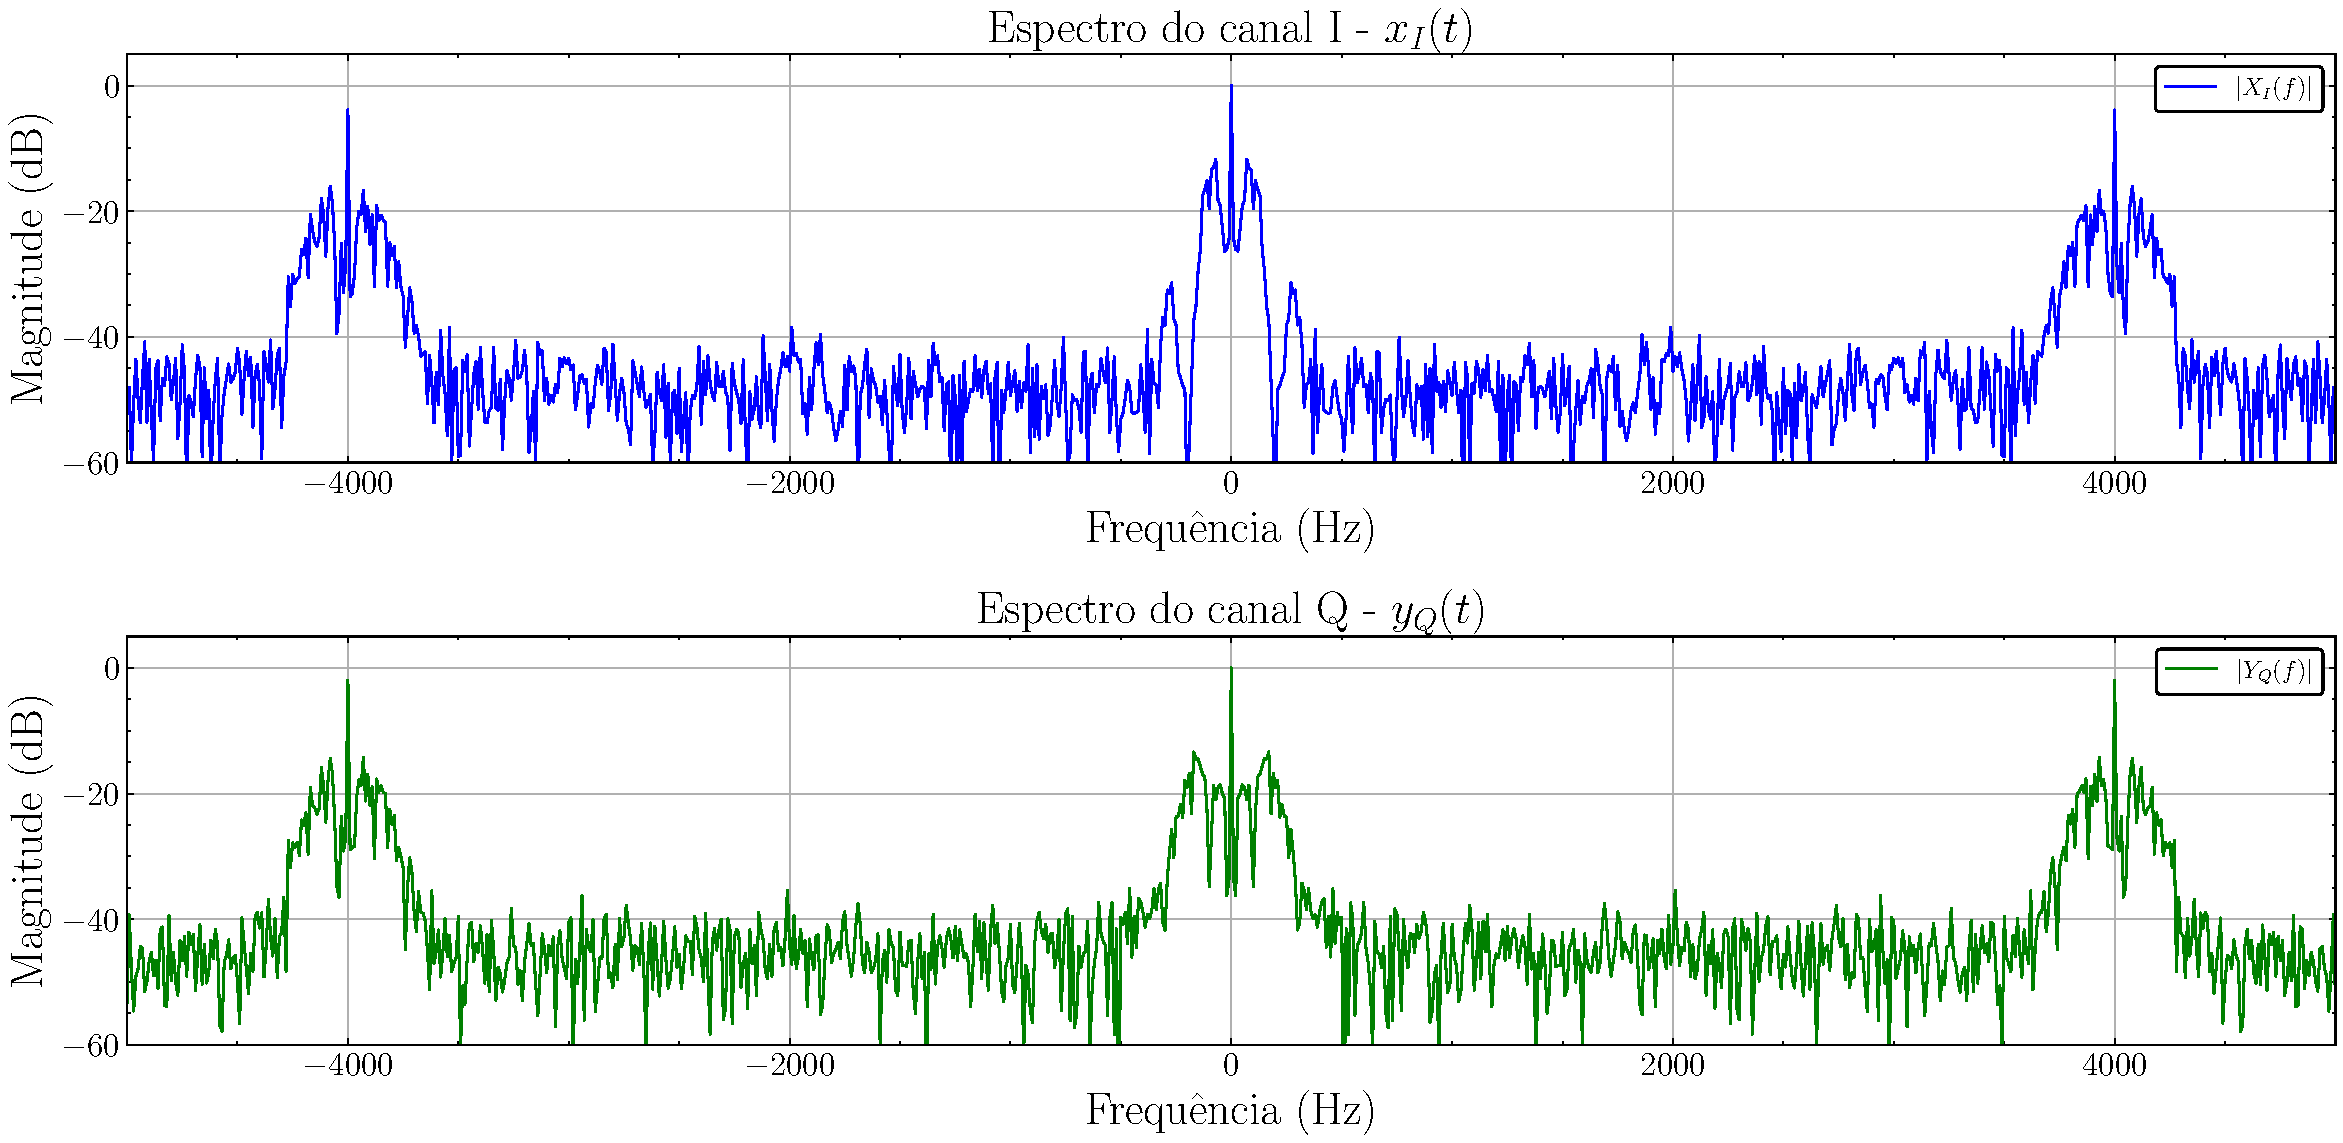
\includegraphics[width=\linewidth]{assets/fft_produtos_com_portadoras.pdf}
\end{figure}


\subsection{Filtragem passa baixa e Filtragem Casada}

Para isolar os sinais em banda base \gls{dIprime} e \gls{dQprime}, é necessário aplicar um \gls{LPF}, para isso utiliza-se um filtro Butterworth (6ª Ordem) com frequência de corte de $1,5$ \gls{khz}, com resposta ao impulso \gls{ht}, que remove as componentes de alta frequência em $2 \cdot \text{\gls{fc}}$ resultantes da multiplicação de demodulação realizada anteriormente \cite{rodrigues_demodulador_2018}.

A \autoref{fig:espectros_filtragem_comparacao} apresenta o espectro dos sinais \gls{dIprime} e \gls{dQprime} antes e após a filtragem passa-baixa, bem como a resposta ao impulso \gls{ht} do filtro, onde é possível observar a remoção das componentes de alta frequência, deixando apenas os sinais em banda base.

\begin{figure}[H]
	\centering
	\caption{Filtragem passa baixa de I e Q}\label{fig:espectros_filtragem_comparacao}
	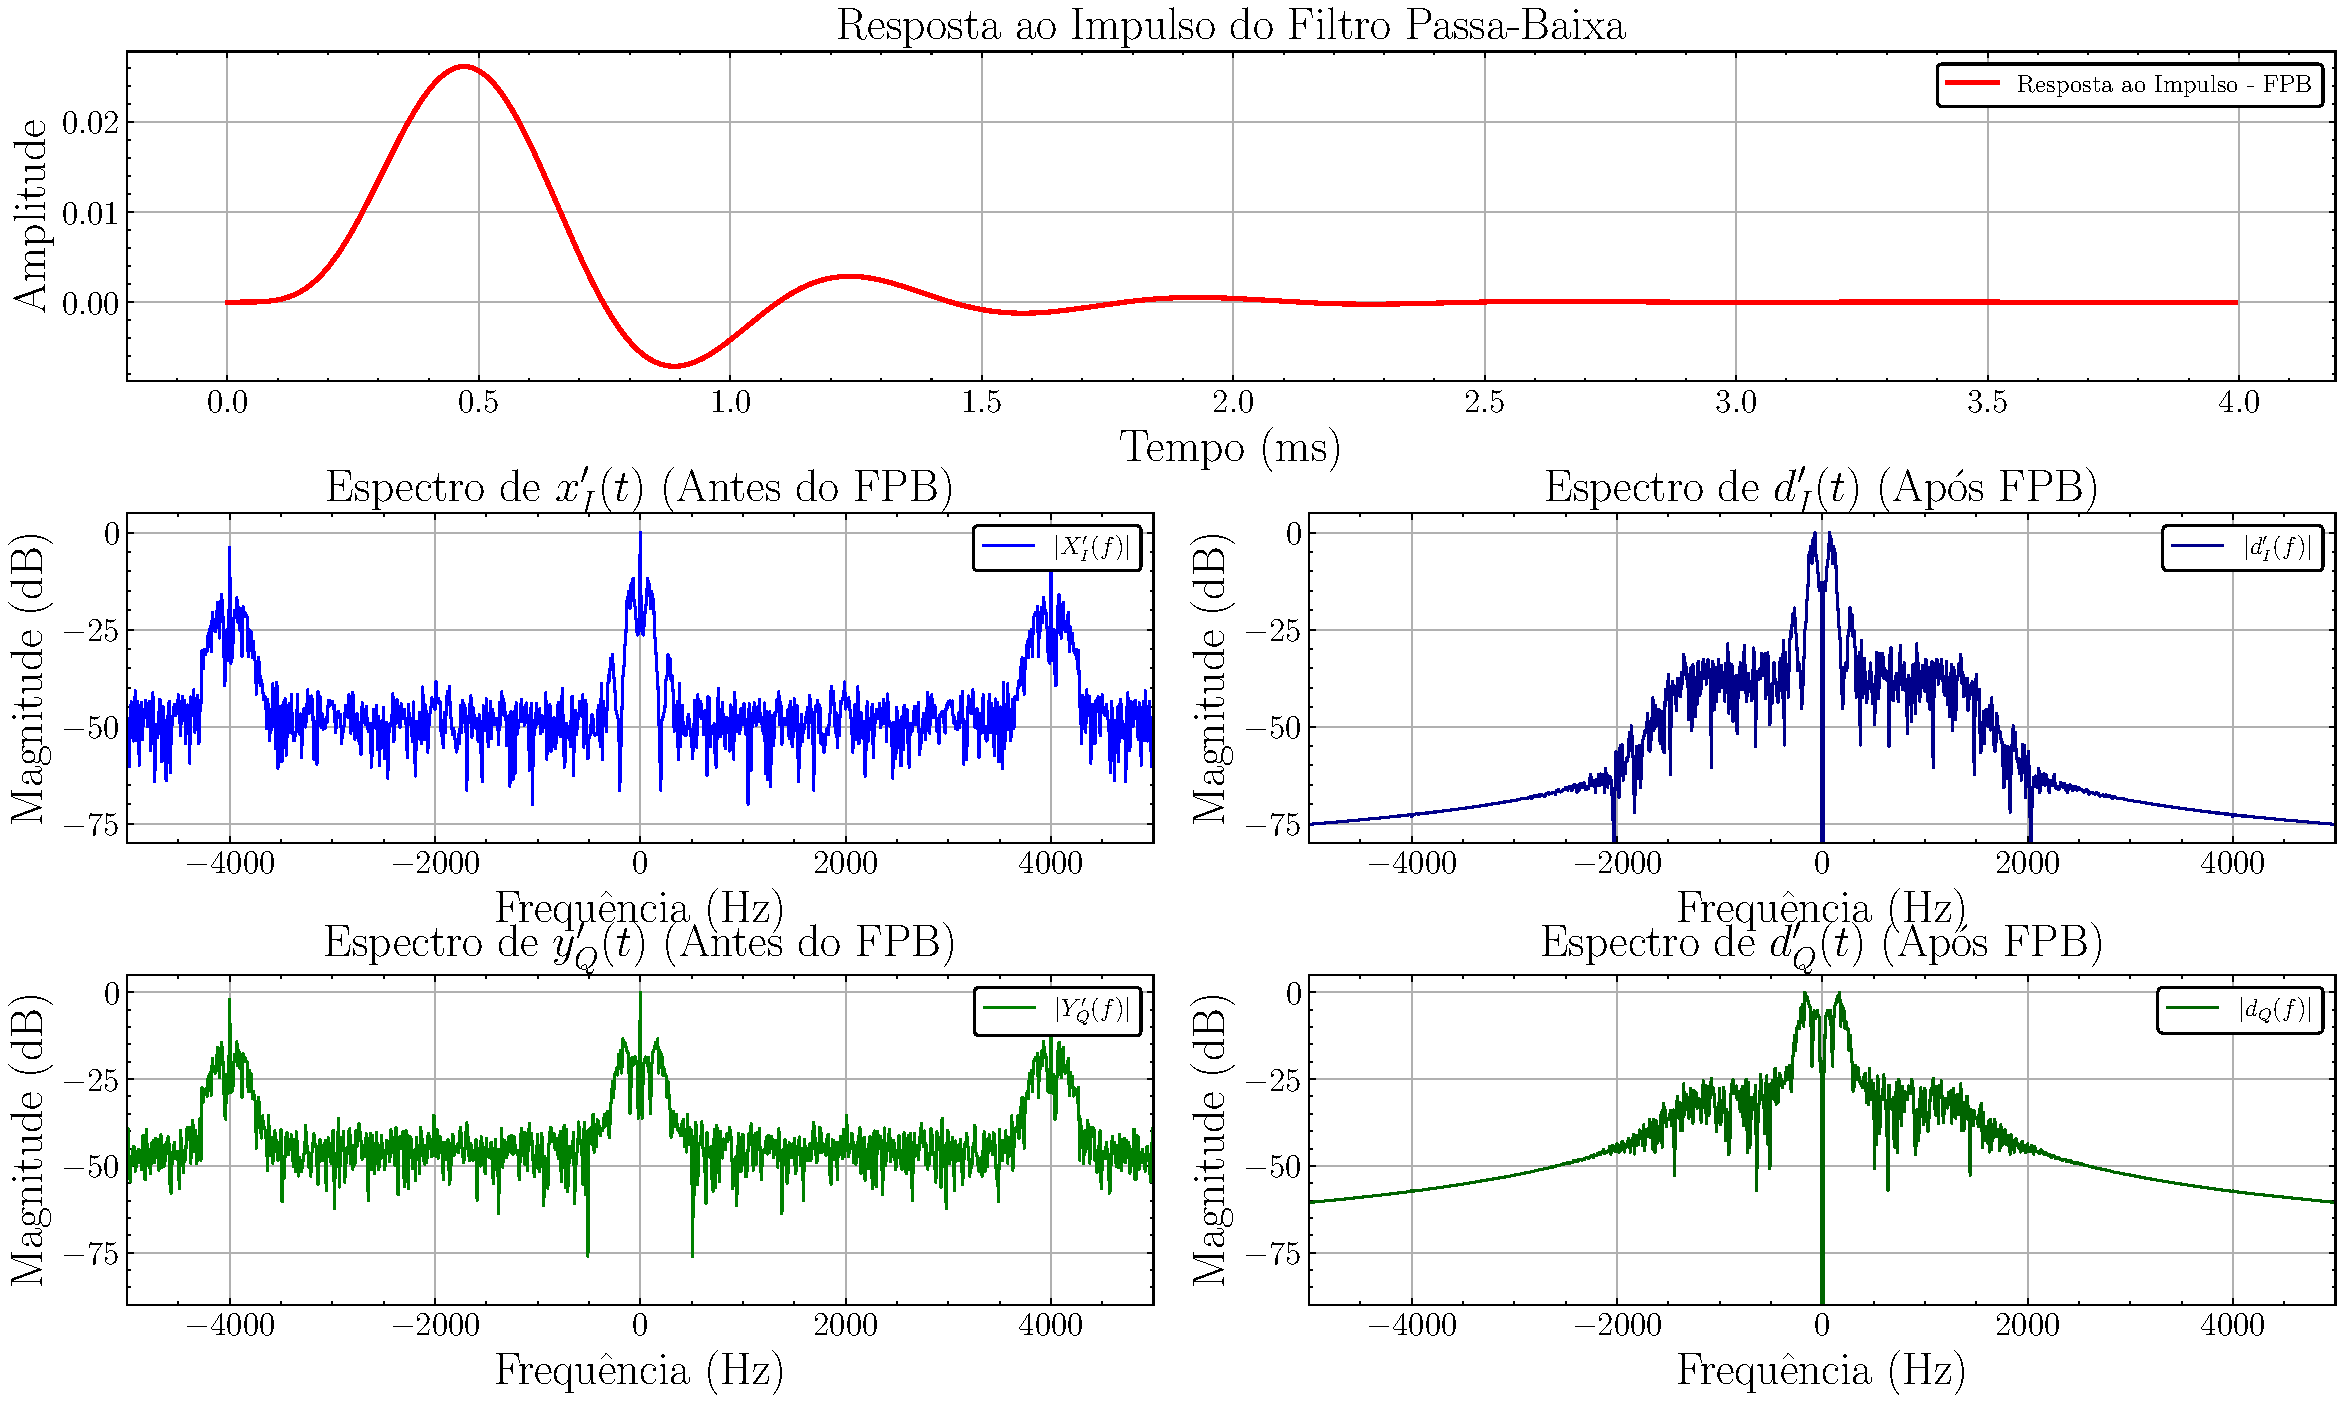
\includegraphics[width=\linewidth]{assets/espectros_filtragem_comparacao.pdf}
    
\end{figure}

\subsection{Filtragem Casada}

Os sinais \gls{dIprime} e \gls{dQprime} em banda base, e já filtrados por um \gls{LPF}, passam por um filtro casado \gls{MF}, que é utilizado para maximizar a relação sinal-ruído (\gls{SNR}). O filtro casado é ajustado para coincidir com o inverso do pulso  \gls{gti} utilizado na formatação do sinal na transmissão \cite{10555531840}. 

O filtro casado é aplicado aos sinais \gls{dIprime} e \gls{dQprime} através da expressão

\vspace{-1em}
\begin{equation}
    \begin{array}{c@{\quad\text{e}\quad}c}
        I'(t) = d_I(t) * g(-t) &
        Q'(t) = d_Q(t) * g(-t)
    \end{array} \text{ .}
\end{equation}


A \autoref{fig:espectros_filtro_casado} apresenta o espectro dos sinais \gls{Iprime} e \gls{Qprime} após a filtragem casada, onde é possível observar a melhoria na relação sinal-ruído e a remoção de componentes indesejadas. 

\begin{figure}[H]
	\centering
	\caption{Filtragem casada de I e Q}\label{fig:espectros_filtro_casado}
	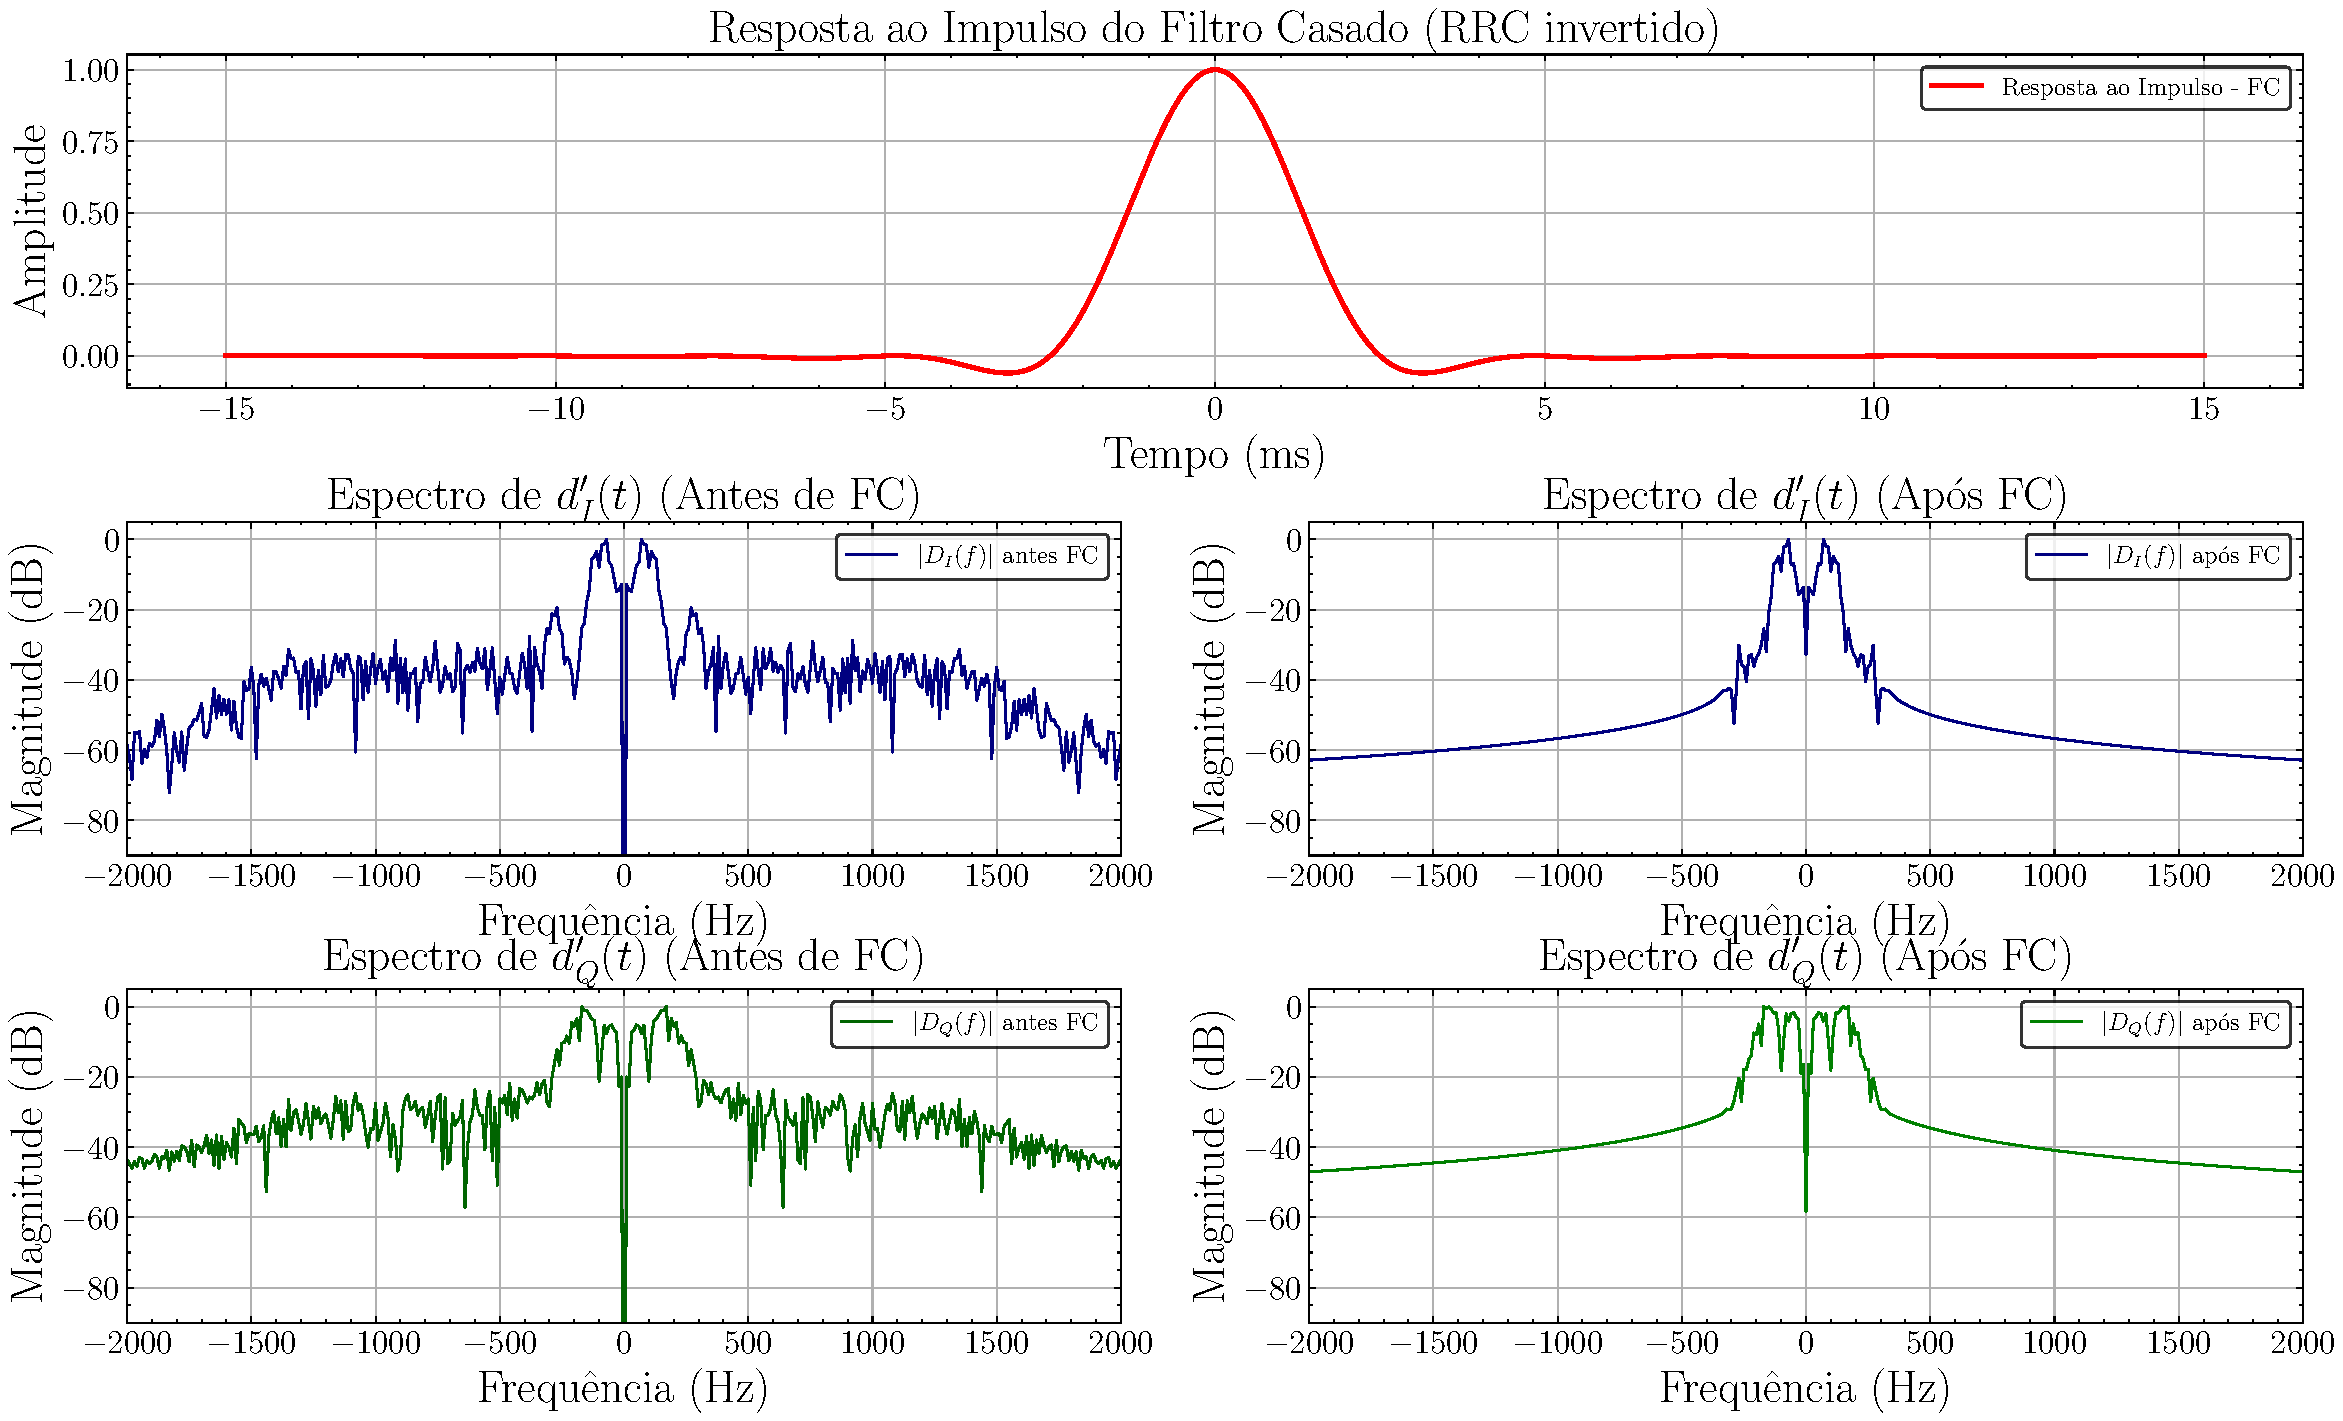
\includegraphics[width=\linewidth]{assets/espectros_filtro_casado.pdf}
\end{figure}


\subsection{Decisão de simbolos}

Uma vez com os sinais \gls{dIprime} e \gls{dQprime} filtrados, considerando sincronismo perfeito, o próximo passo é a decisão dos sinais em instantes de \gls{Tb} (instante ótimo de decisão) a partir de um delay inicial \gls{tau}, para recuperar os símbolos transmitidos. O processo de decisão pode ser expresso como

\vspace{-1em}
\begin{equation}
    \begin{array}{c@{\quad\text{e}\quad}c}
        I'[n] = d'_I(n \cdot T_b + \tau) & Q'[n] = d'_Q(n \cdot T_b + \tau)
    \end{array} \text{ ,}
\end{equation}

\noindent onde \gls{n} é o índice de amostra, \gls{Tb} é o tempo de bit $1/R_b$ e \gls{tau} é o atraso inicial da decisão. A \autoref{fig:sinais_amostrados_pos_filtro_casado} apresenta os sinais amostrados \gls{Inprime} e \gls{Qnprime}. 

\begin{figure}[H]
	\centering
	\caption{Decisão de I e Q}\label{fig:sinais_amostrados_pos_filtro_casado}
	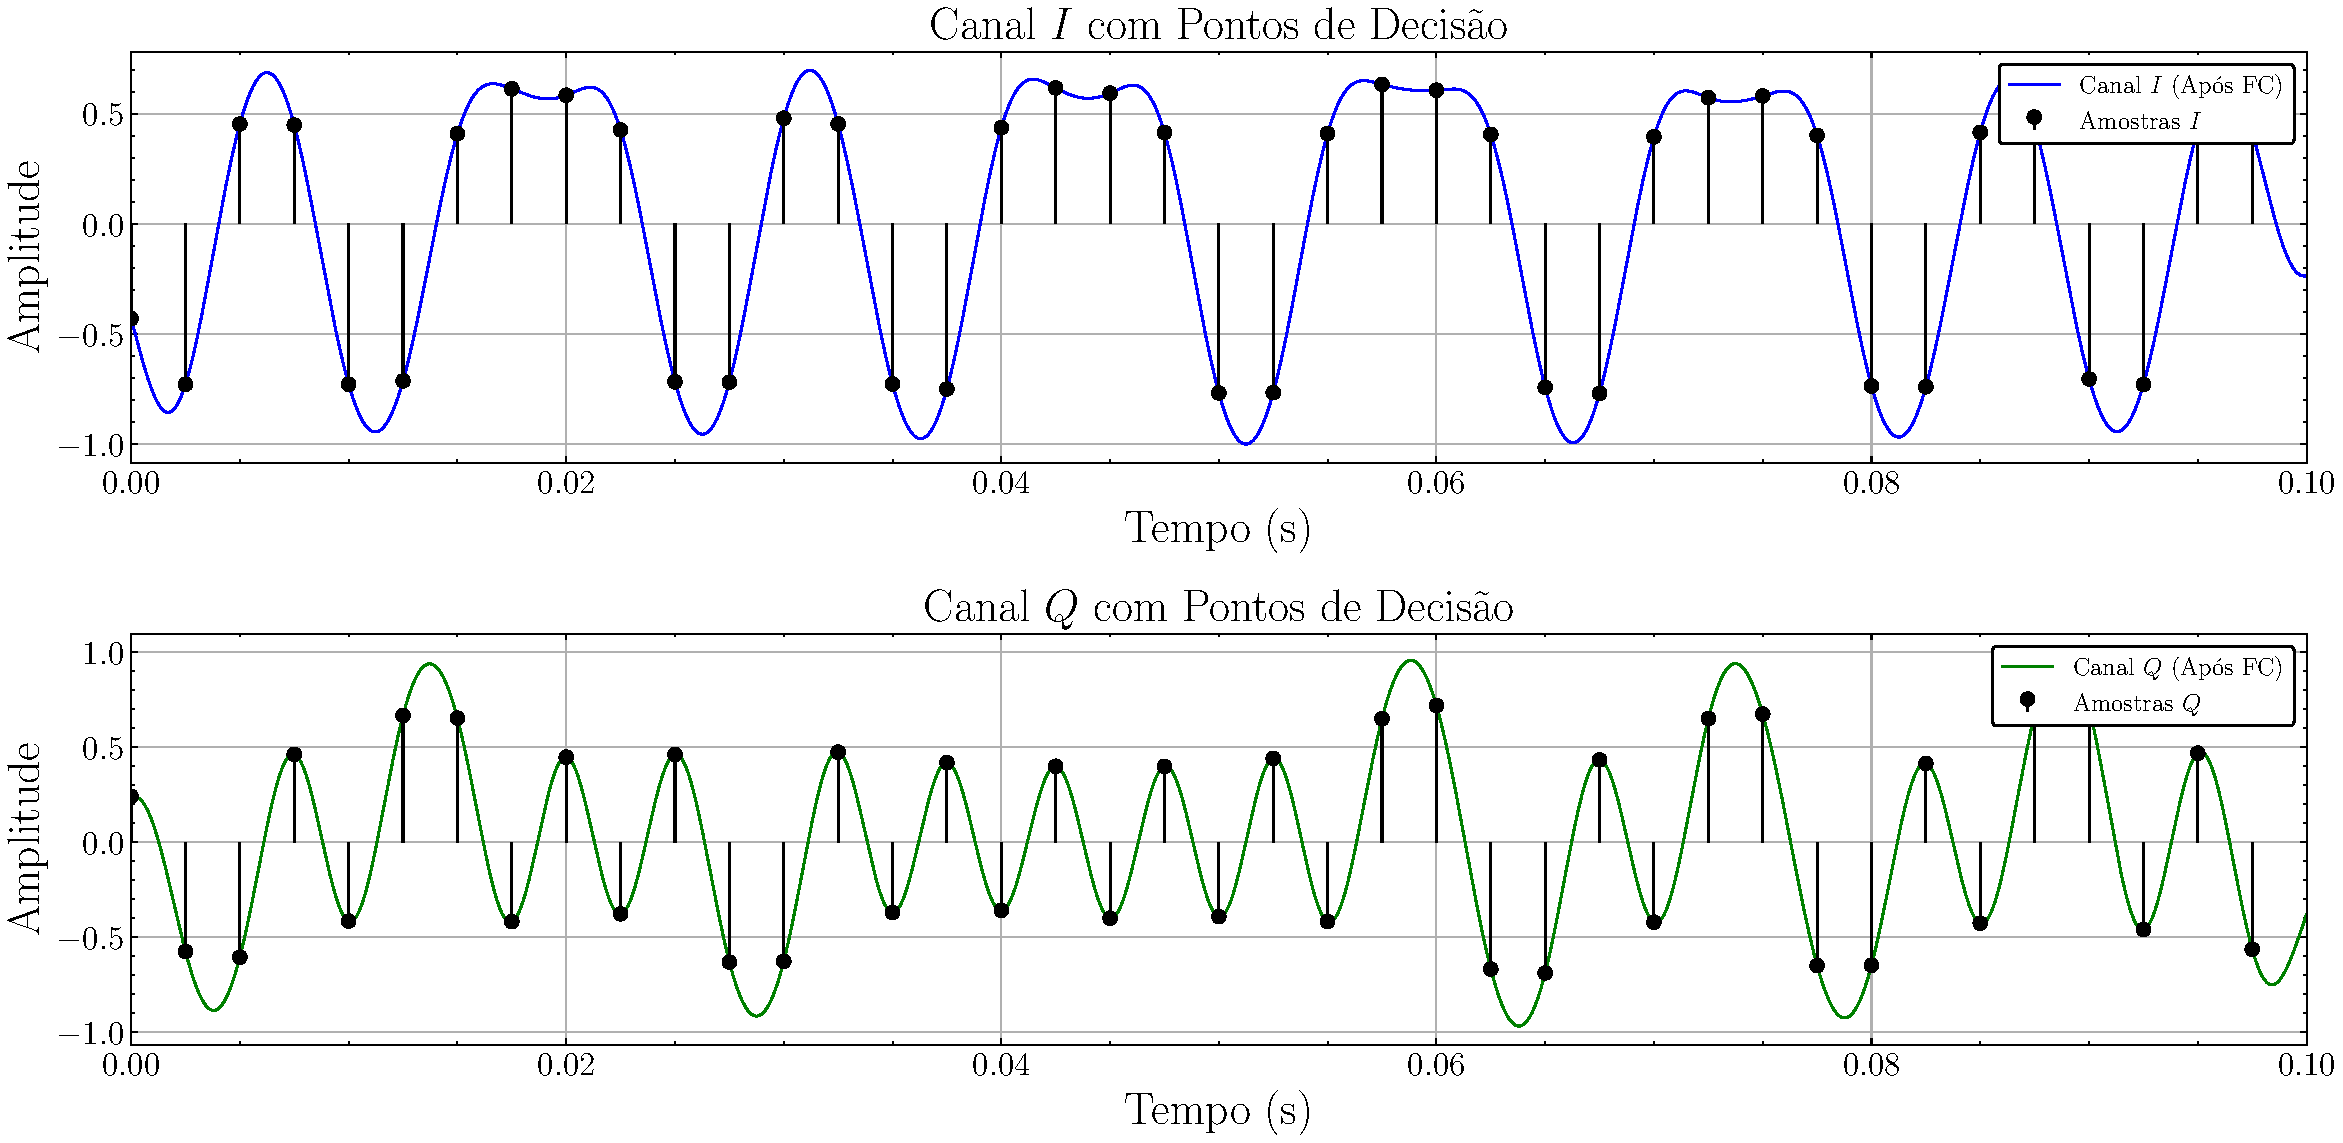
\includegraphics[width=\linewidth]{assets/sinais_amostrados_pos_filtro_casado.pdf}
    
\end{figure}

Os valores amostrados \gls{Inprime} e \gls{Qnprime} são então decididos, isto é, quantizados para valores discretos, correspondendo aos símbolos transmitidos. O mapeamento dos pares pode ser expressado como

\begin{equation} 
    I'[n] = \begin{cases}
    +1, & \text{se } I'[n] \geq 0 \\
    -1, & \text{se } I'[n] < 0
    \end{cases}, \quad
    Q'[n] = \begin{cases}
    +1, & \text{se } Q'[n] \geq 0 \\
    -1, & \text{se } Q'[n] < 0
    \end{cases} \text{ ,}
\end{equation}

\noindent onde \gls{Inprime} e \gls{Qnprime} são os vetores simbolo. A \autoref{fig:comparacao_bits_recuperados} apresenta os simbolos decididos nos vetores \gls{Inprime} e \gls{Qnprime} após o processo de quantização, em comparação com os vetores originais \gls{In} e \gls{Qn} transmitidos.

\begin{figure}[H]
	\centering
	\caption{Comparação dos vetores IQ decididos}\label{fig:comparacao_bits_recuperados}
	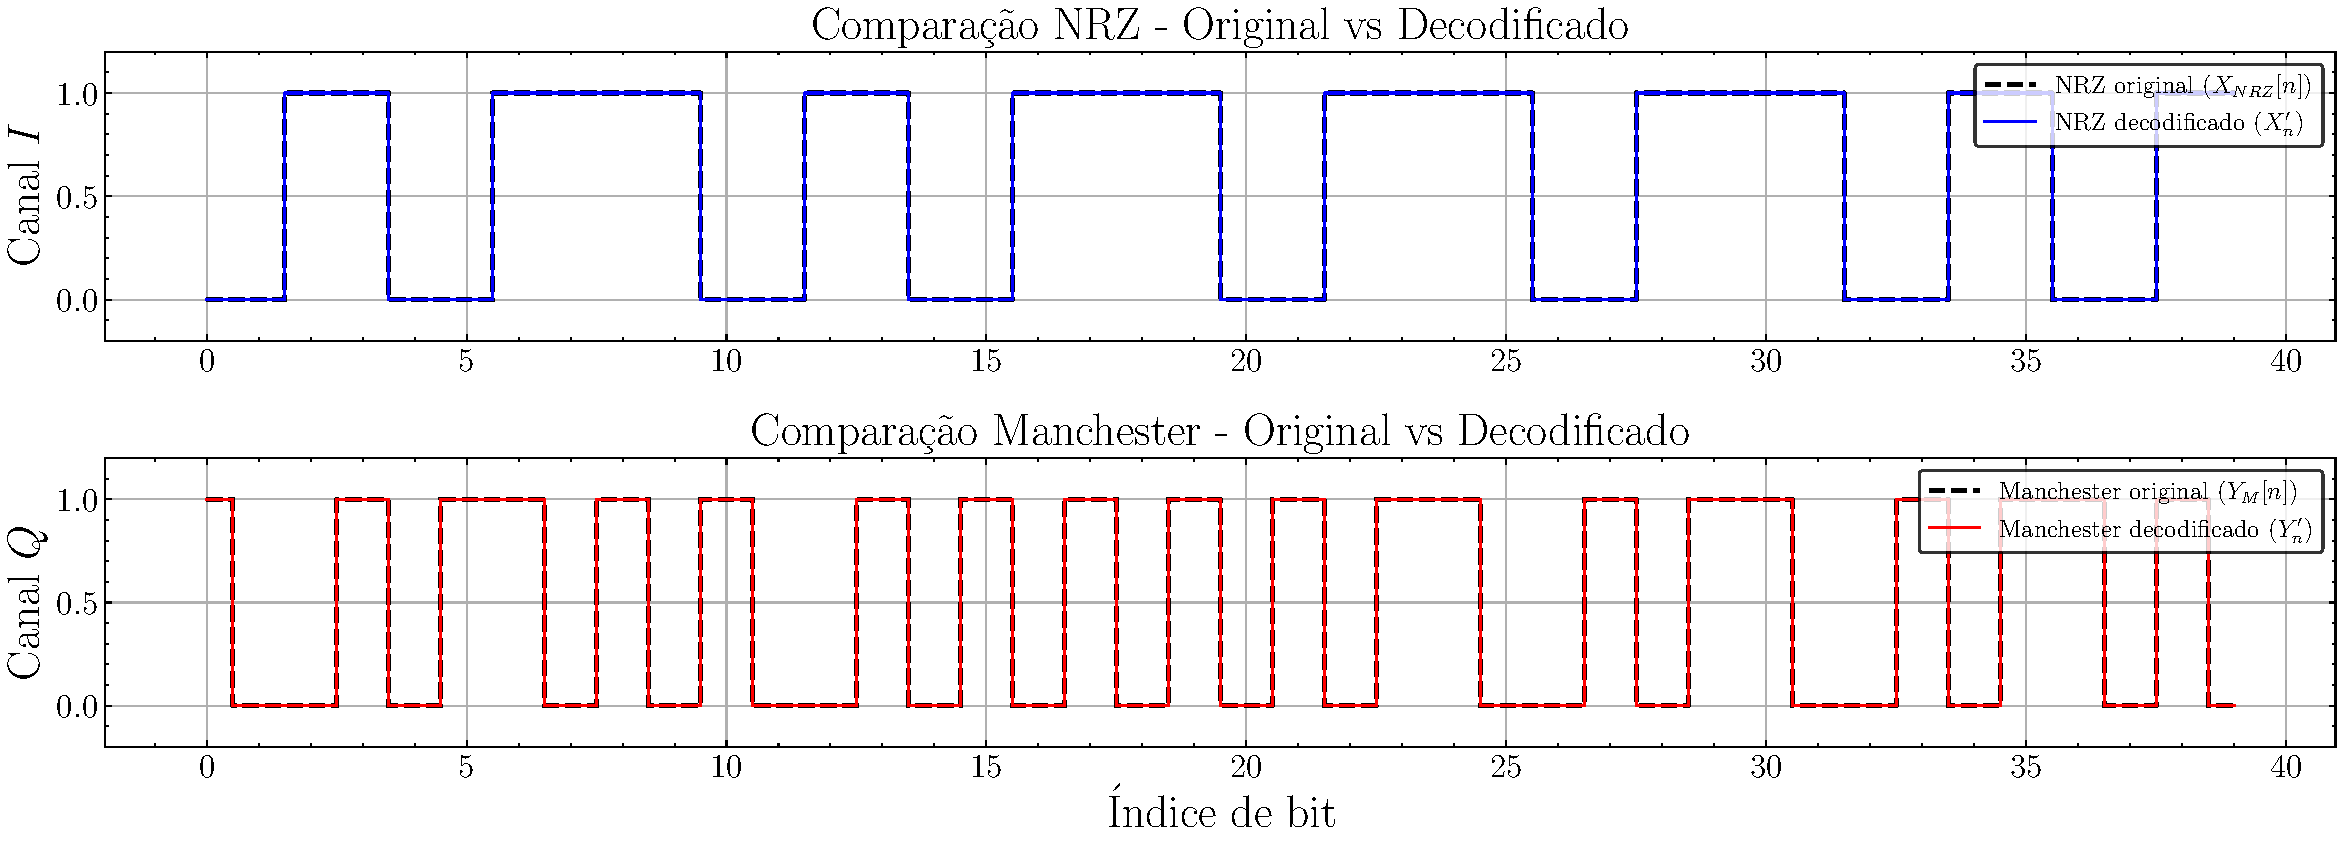
\includegraphics[width=\linewidth]{assets/comparacao_bits_recuperados.pdf}
\end{figure}

\subsection{Decodificador de linha}

Após a decisão dos símbolos, os vetores \gls{Inprime} e \gls{Qnprime} precisam ser convertidos de volta para a representação original dos bits. Para isso, são aplicadas as técnicas de decodificação de linha inversas às utilizadas na transmissão: \gls{NRZ} para o canal \gls{cI} e \gls{Manchester} para o canal \gls{cQ}. A decodificação \gls{NRZ} é realizada mapeando os valores '+1' para o bit '1' e '-1' para o bit '0', conforme

\begin{equation}
    X'[n] = 
    \begin{cases}
    1, & \text{se } I'[n] = +1 \\
    0, & \text{se } I'[n] = -1
    \end{cases} \text{ ,}
\end{equation}


\noindent resultando no vetor de bits \gls{Xnprime} correspondente ao canal \gls{cI}. O mesmo processo é aplicado ao canal \gls{cQ}, onde a decodificação \gls{Manchester} mapeia os pares de valores '+1,-1' para o bit '1' e '-1,+1' para o bit '0', conforme

\begin{equation}
    Y'[n] = 
    \begin{cases}
    1, & \text{se } Q'[n] = +1,-1 \\
    0, & \text{se } Q'[n] = -1,+1
    \end{cases} \text{ ,}
\end{equation}

\noindent resultando no vetor de bits \gls{Ynprime} correspondente ao canal \gls{cQ}. 

\subsection{Desembaralhador}

Após o processo de decodificação de linha, os dados vetores de bits \gls{Xnprime} e \gls{Ynprime} ainda encontram-se embaralhados, então é necessário realizar o desembaralhamento para restaurar a sequência original dos bits antes da decodificação convolucional \cite{cnes_services_and_message_formats_ed2_rev2_2006}.

O desembaralhador utiliza a mesma estrutura lógica do embaralhador, porém executando a operação inversa de reorganização dos bits, com base em regras posicionais dependentes do índice dos bits \gls{n}. A \autoref{fig:desembaralhador} apresenta o diagrama de blocos do desembaralhador utilizado no \gls{PTT-A3}, que refaz a ordenação dos bits após a demodulação \cite{rodrigues_demodulador_2018}.

\begin{figure}[H]
\centering
\caption{Desembaralhador de dados para o ARGOS-3}\label{fig:desembaralhador}
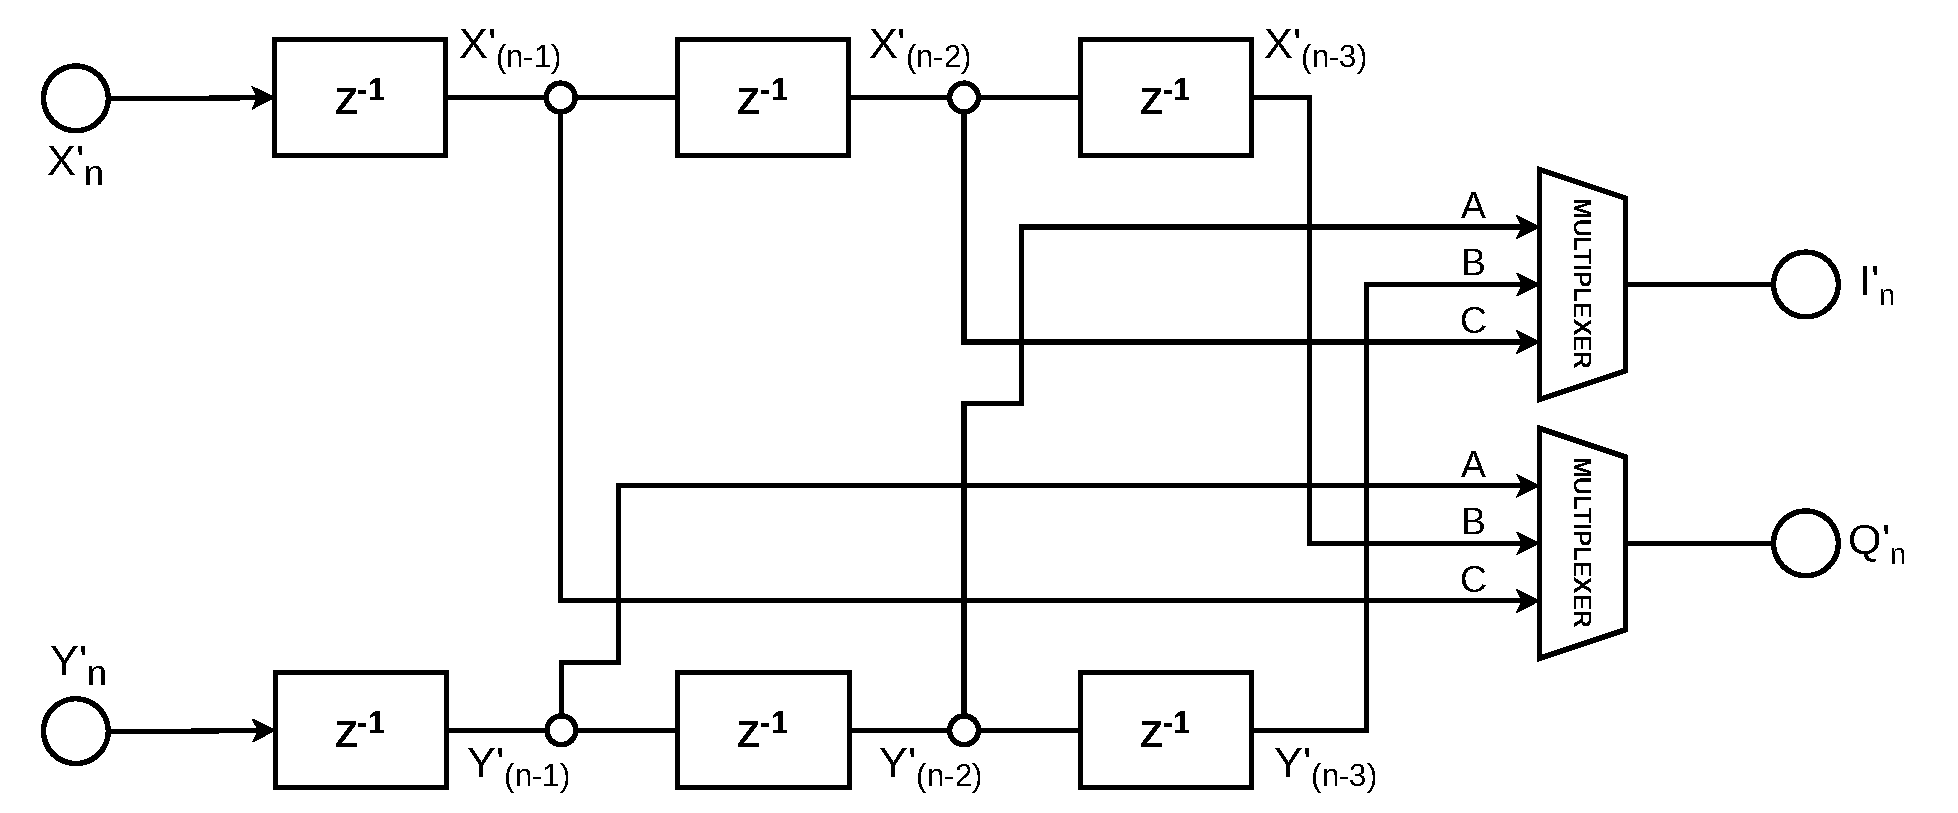
\includegraphics[width=\linewidth]{assets/desembaralhador.pdf}
\end{figure}

O processo de desembaralhamento retorna os vetores de bit, \gls{vt0prime} e \gls{vt1prime}, que correspondem aos dados codificados nos canais \gls{cI} e \gls{cQ}, respectivamente.

\subsection{Decodificador convolucional}

Após o desembaralhamento, os vetores \gls{vt0prime} e \gls{vt1prime} estão prontos para a decodificação convolucional. O algoritmo mais popularmente utilizado para essa etapa é o algoritmo de Viterbi, que implementa a decodificação \gls{MLD} para códigos convolucionais, calculando o caminho mais provável através de \gls{Hamming} para a mensagem recebida em relação à mensagem possível \cite{cnes_services_and_message_formats_ed2_rev2_2006, rodrigues_demodulador_2018}.

No padrão \gls{ARGOS-III}, o código convolucional utilizado segue o padrão \gls{CCSDS} 131.1-G-2, que, por sua vez, possui uma distância livre conhecida de $\text{\gls{dfree}} = 10$. Quanto maior for o valor de \gls{dfree}, maior será a robustez do código e sua capacidade de detectar e corrigir erros.

\noindent Assim, conforme o comparativo ilustrado na \autoref{fig:decodificador_convolucional} entre a transmissão \gls{QPSK} sem codificação e com codificação convolucional, o uso desta técnica na transmissão do sinal permite operar em valores de \gls{EbN0} menores em relação a não utilização do codificador, para a \gls{BER} visada pelo sistema, permitindo uso em ambientes com maior ruído para a mesma taxa de erro desejada.

\begin{figure}[H]
	\centering
	\caption{Comparação de BER vs \gls{EbN0} utilizando codificação convolucional}\label{fig:decodificador_convolucional}
	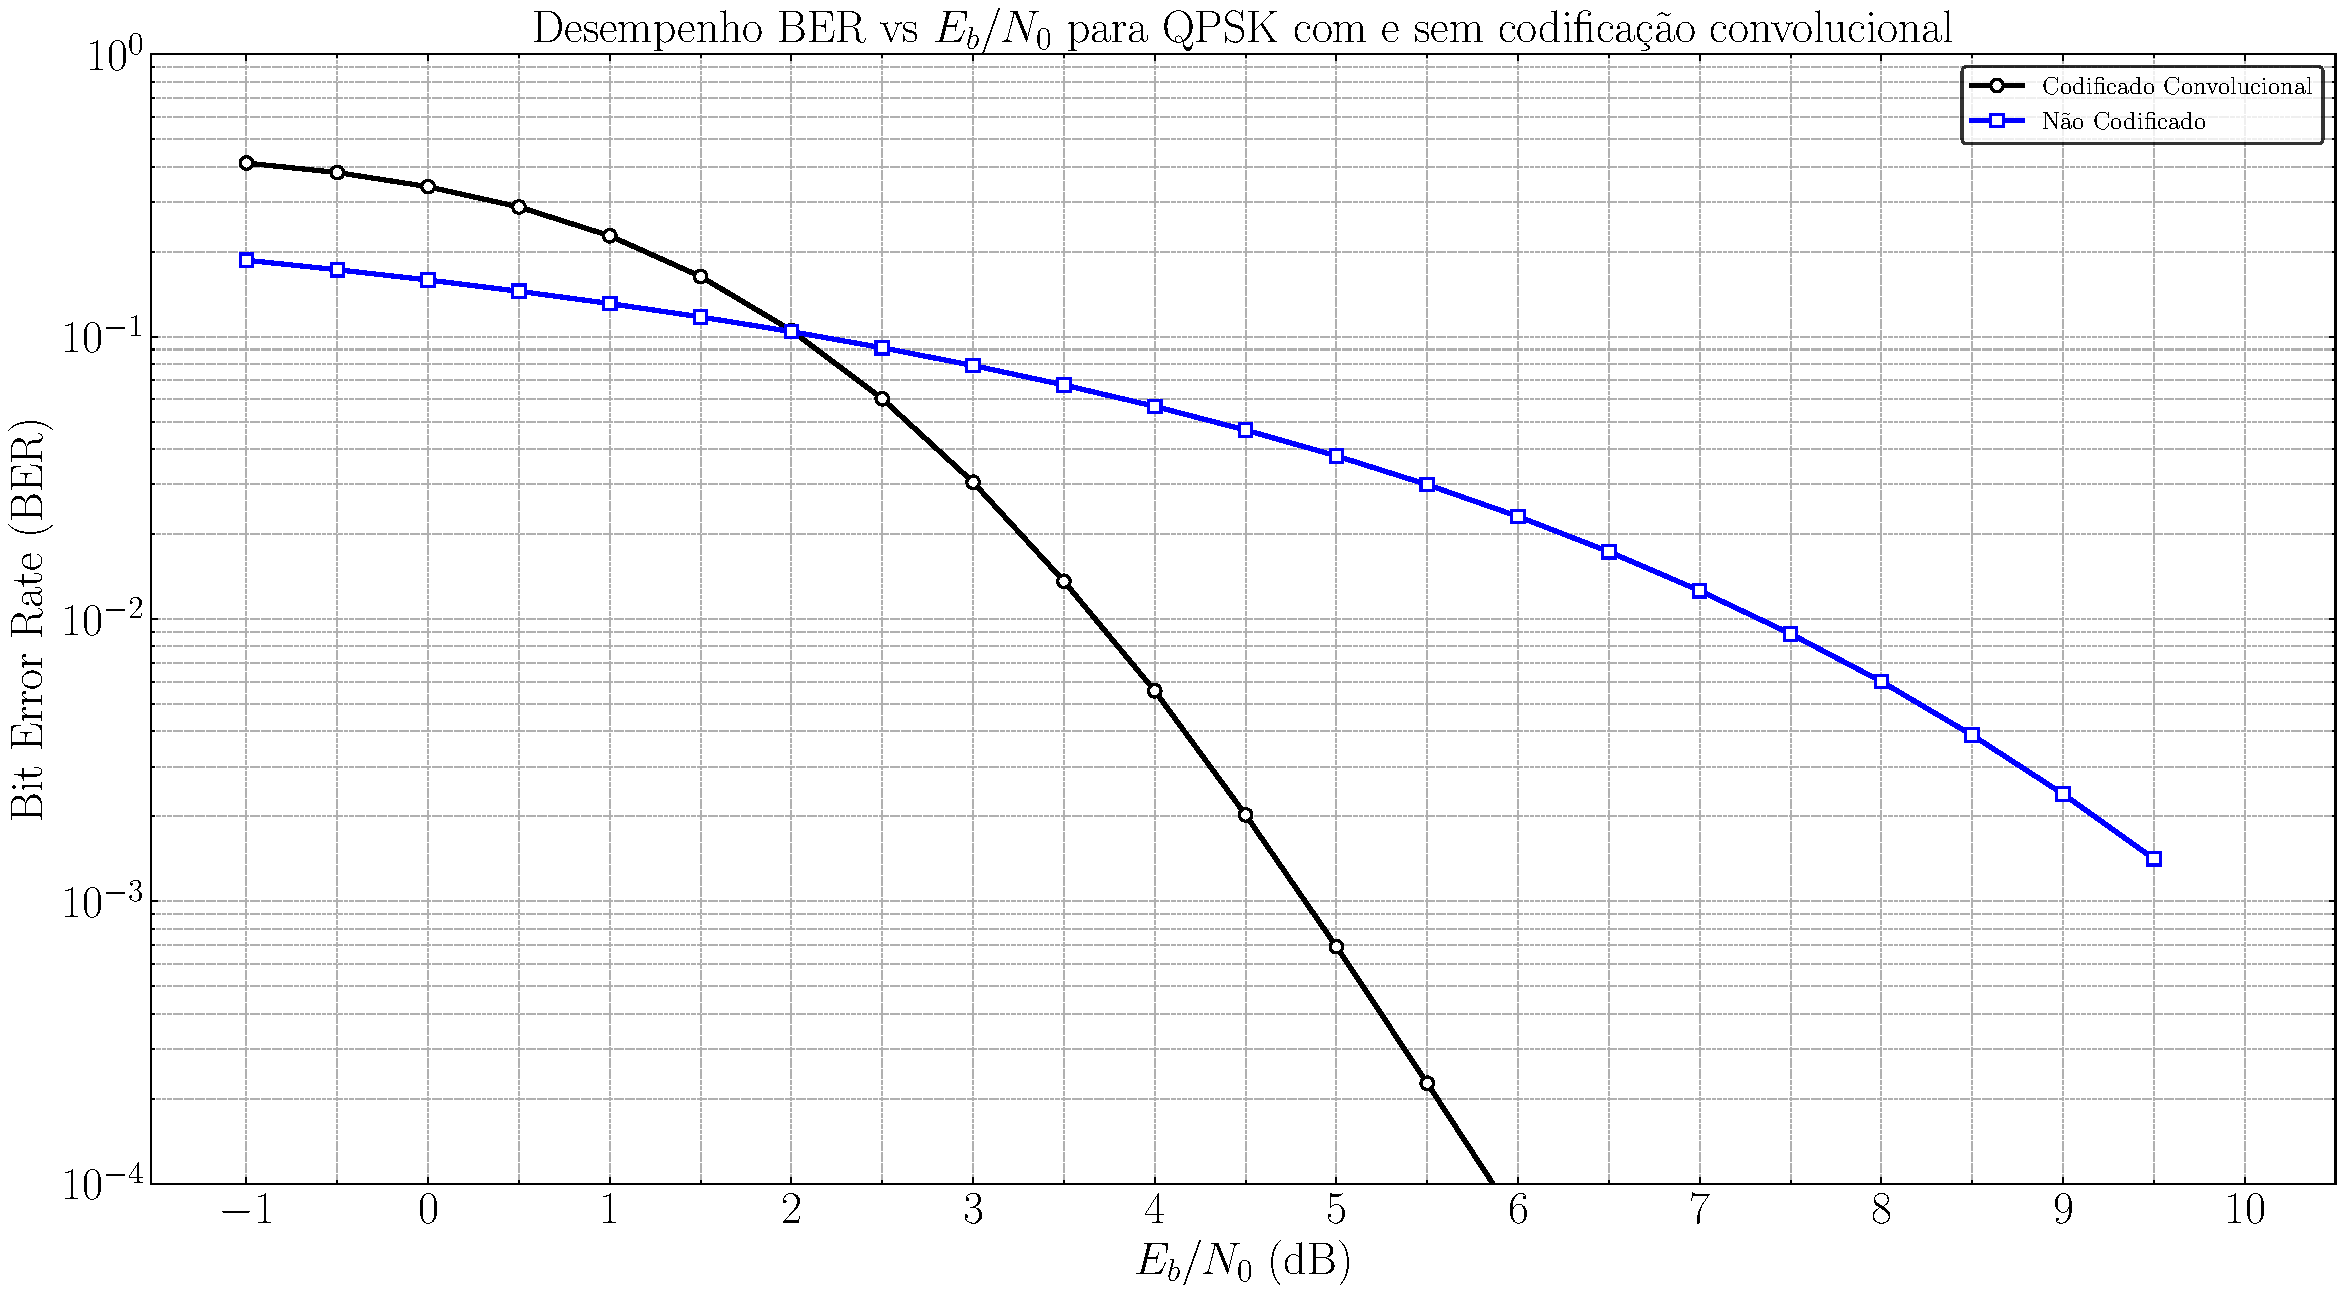
\includegraphics[width=\linewidth]{assets/convolutional.pdf}
\end{figure}
\chapter{DESENVOLVIMENTO E RESULTADOS}\label{cap:desenvolvimento}

Este capítulo apresenta a implementação do sistema de comunicação digital proposto, detalhando cada etapa do processo, desde a geração dos bits até a recuperação do datagrama no receptor. A seguir, são descritas as principais componentes do sistema, incluindo a cadeia de transmissão, o canal de comunicação com ruído adicionado, a detecção de portadora e a cadeia de recepção.

\section{CADEIA DE TRANSMISSÃO}\label{sec:transmissao}

A primeira etapa do sistema é a geração da sequência de bits que compõem o datagrama ARGOS-3, conforme descrito na Seção \ref{sec:datagrama}. Essa sequência é multiplexada com um preâmbulo para permitir a sincronização de simbolos no receptor. Em seguida, os bits são codificados utilizando codificação de linha para melhorar as caracteristicas espectrais do sinal modulado, como detalhado na Seção \ref{sec:line_coding}.

\subsection{Sequência de transmissão}\label{sec:geracao_bits}

O primeiro passo na cadeia de transmissão é a geração da sequência de bits que compõem o datagrama \gls{ARGOS-III}, conforme ilustrado na \autoref{fig:datagrama_time}, para a montagem do datagrama é necessário o número de identificação da PCD, \gls{ipcd}, e os dados que serão transmitidos (payload), conforme detalhado na seção \ref{sec:datagrama}, desta forma, o comprimento da mensagem \gls{Tm}, o campo de identificação da PCD \gls{pcdid} e a cauda do datagrama \gls{Em} podem ser calculados. 

\begin{figure}[H]
	\centering
	\caption{Streambits do datagrama ARGOS-3}\label{fig:datagrama_time}
	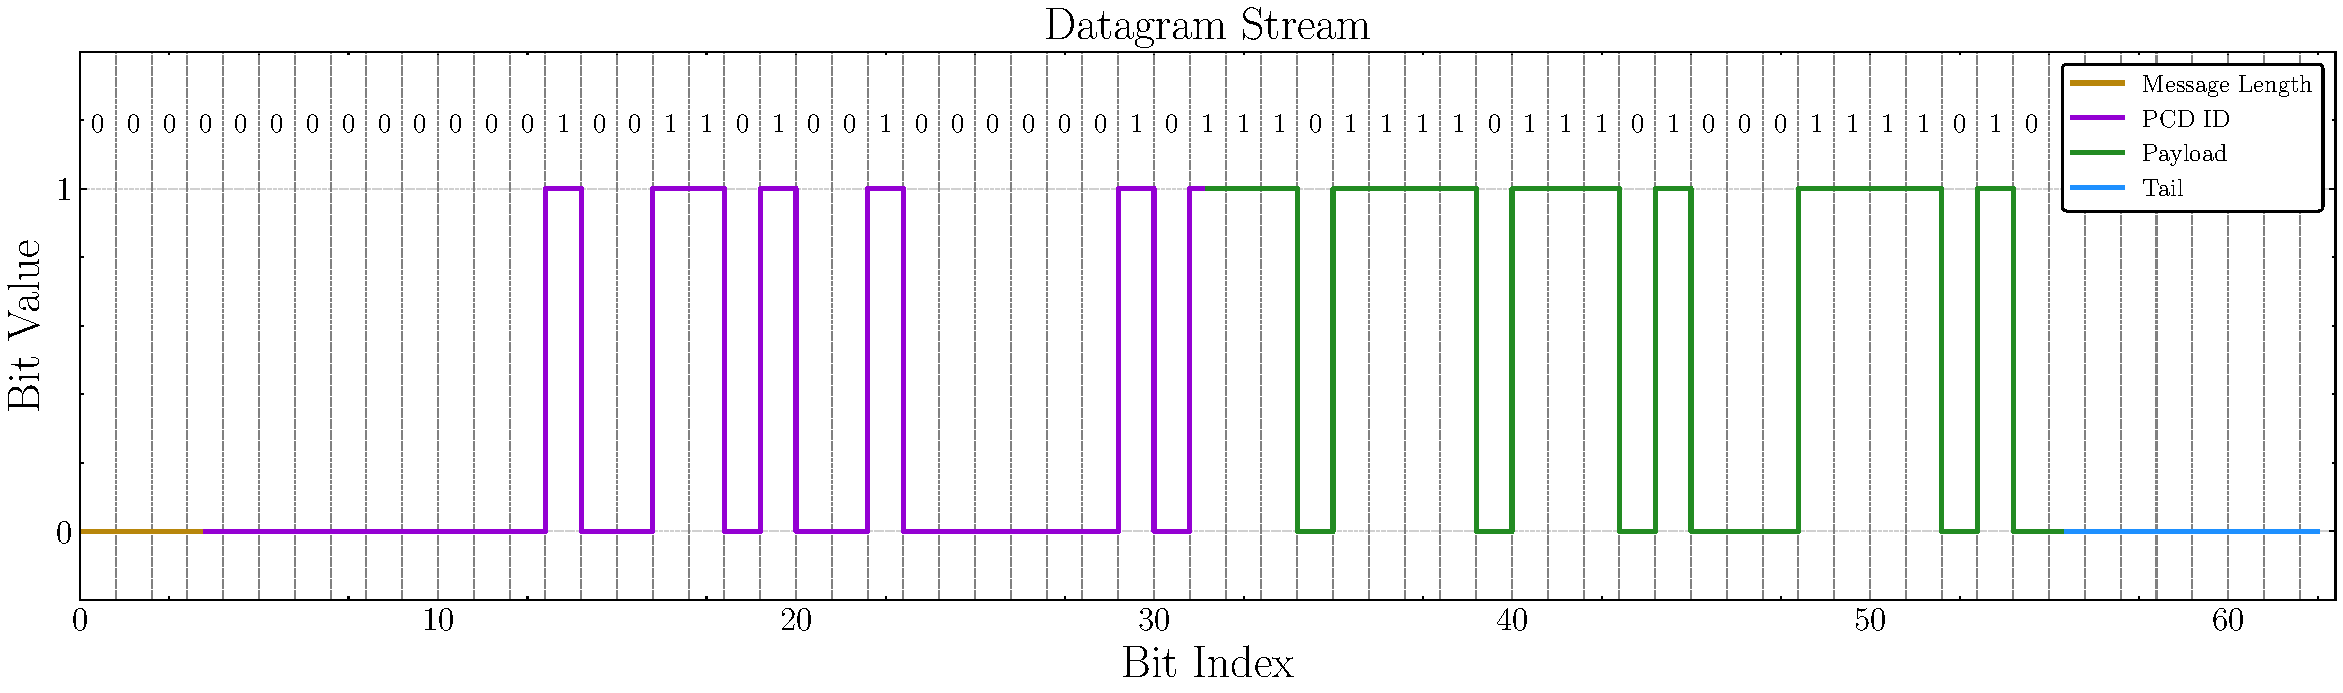
\includegraphics[width=\linewidth]{assets/cap3/transmitter_datagram_time.pdf}
\end{figure}

Após a montagem dos bits \gls{ut} do datagrama, os mesmos são codificados utilizando codificação convolucional, conforme detalhado na seção \ref{sec:conv_coding}, resultando nos vetores de bits \gls{vt0} e \gls{vt1}, que por sua vez são embaralhados resultando nas sequências \gls{Xn} e \gls{Yn} para os canais \gls{cI} e \gls{cQ}, respectivamente, o processo de codificação convolucional aplicado no vetor \gls{ut} é ilustrado na \autoref{fig:transmitter_conv_time}.

\begin{figure}[H]
	\centering
	\caption{Codificação convolucional do datagrama ARGOS-3}\label{fig:transmitter_conv_time}
	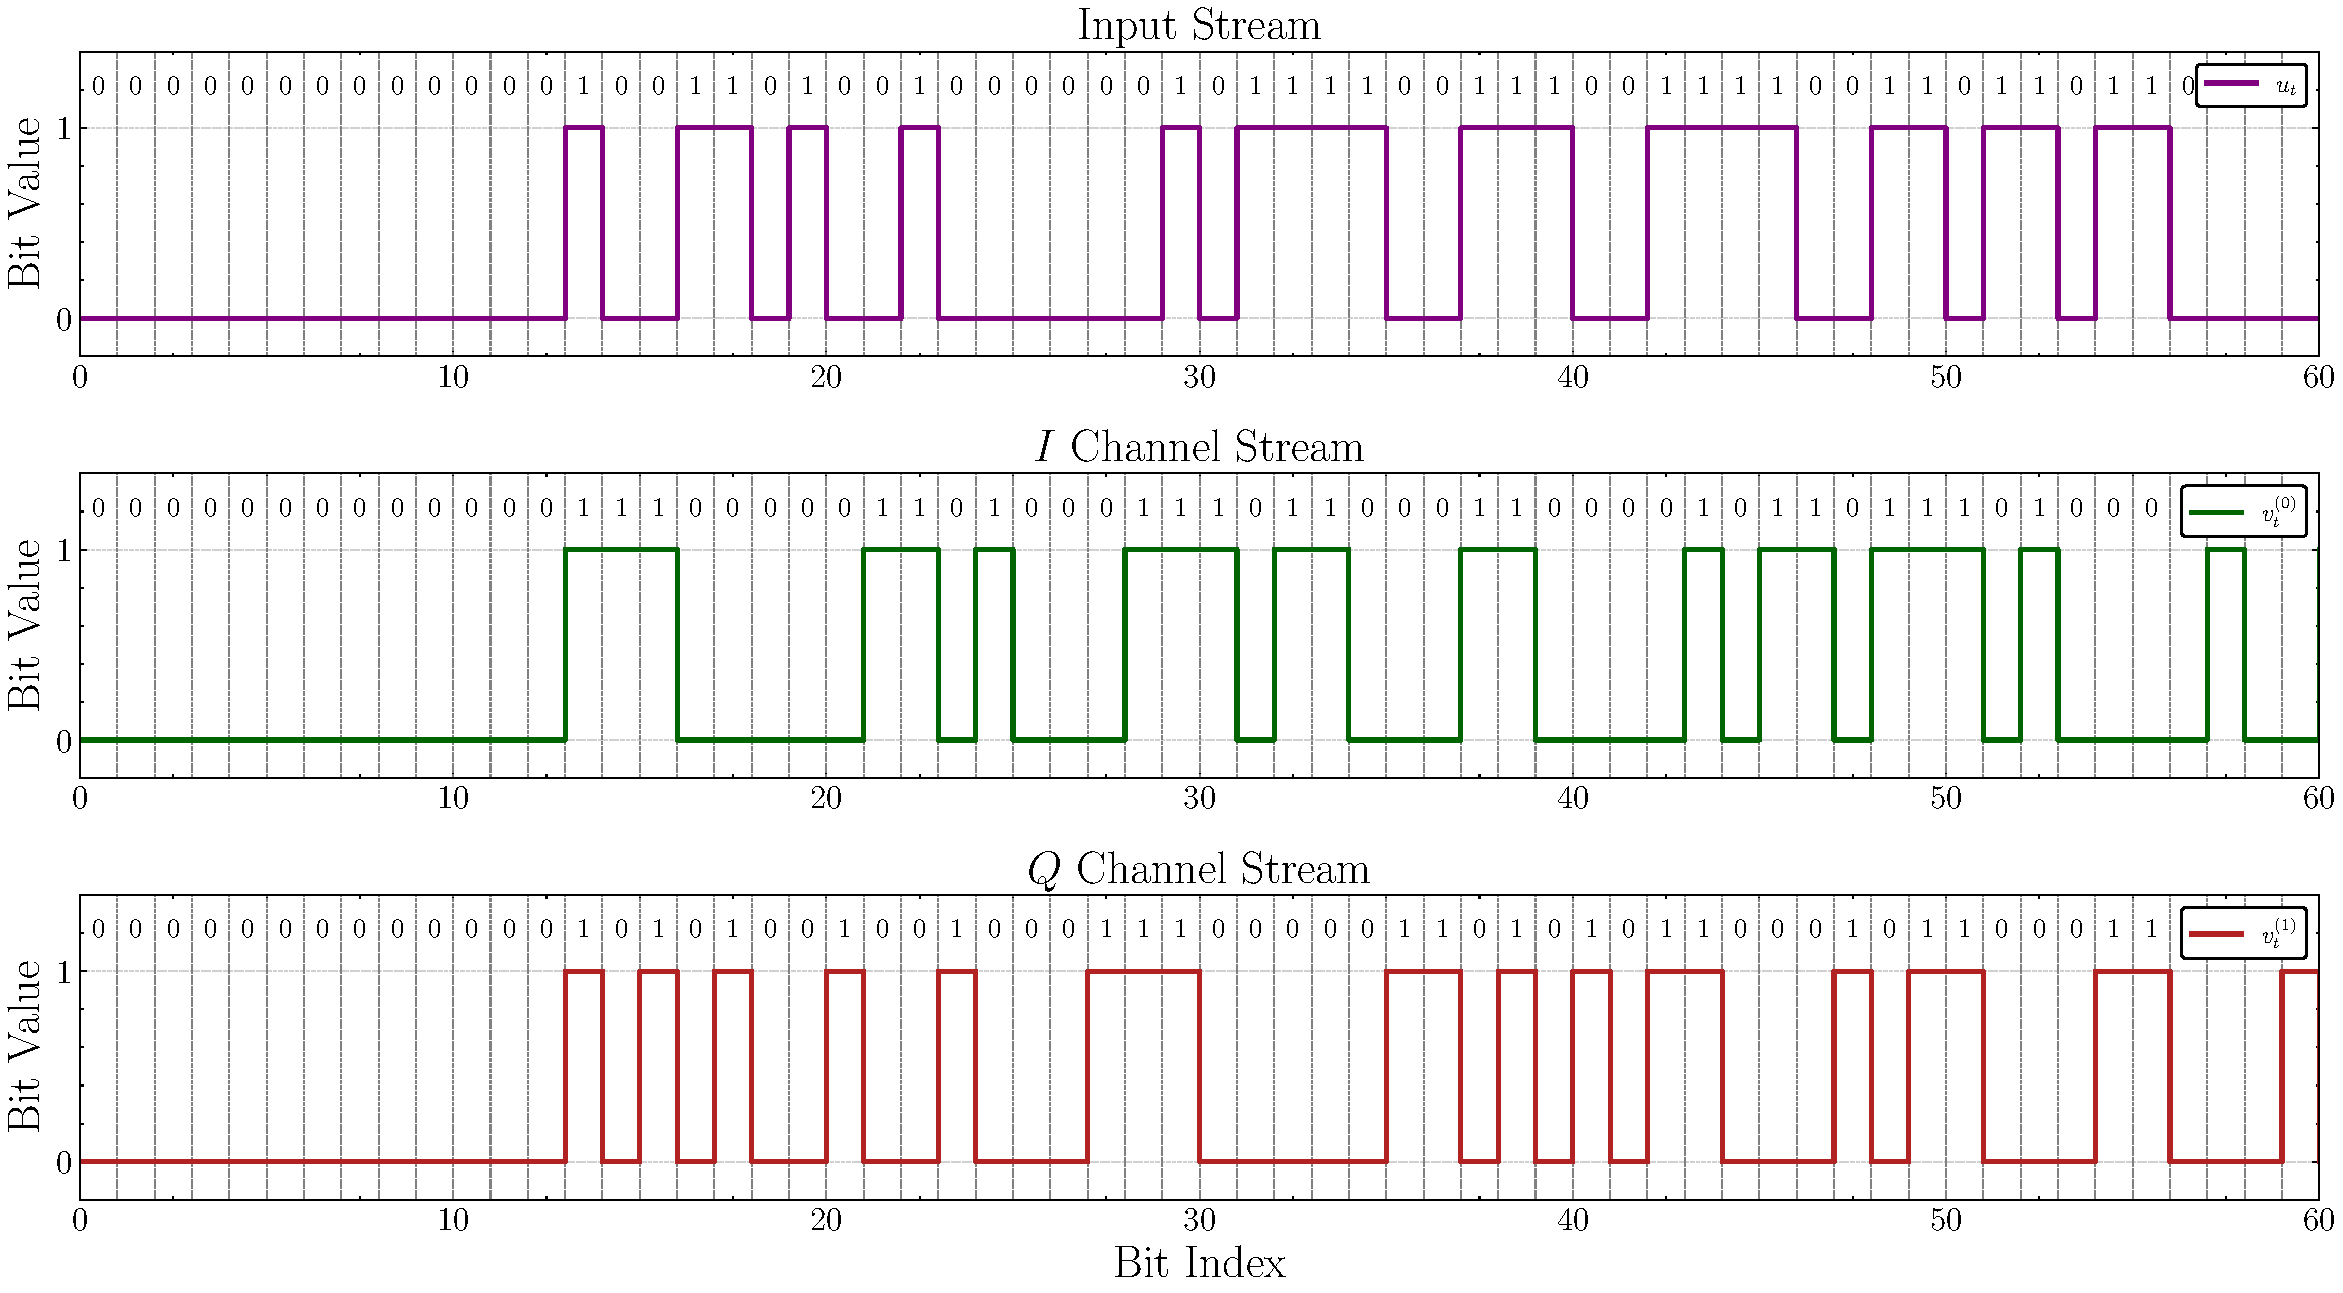
\includegraphics[width=\linewidth]{assets/cap3/transmitter_conv_time.pdf}
\end{figure}

As sequências \gls{Xn} e \gls{Yn} já embaralhadas, são então multiplexadas com o preâmbulo \gls{SIn} e \gls{SQn} dos canais \gls{cI} e \gls{cQ} respectivamente, gerados conforme apresentado na seção \ref{sec:preambulo}. A adição das sequências é fundamental para permitir a sincronização de símbolos no receptor, esse processo é ilustrado na \autoref{fig:mux_time} abaixo.

\begin{figure}[H]
	\centering
	\caption{Multiplexação com preâmbulo}\label{fig:mux_time}
	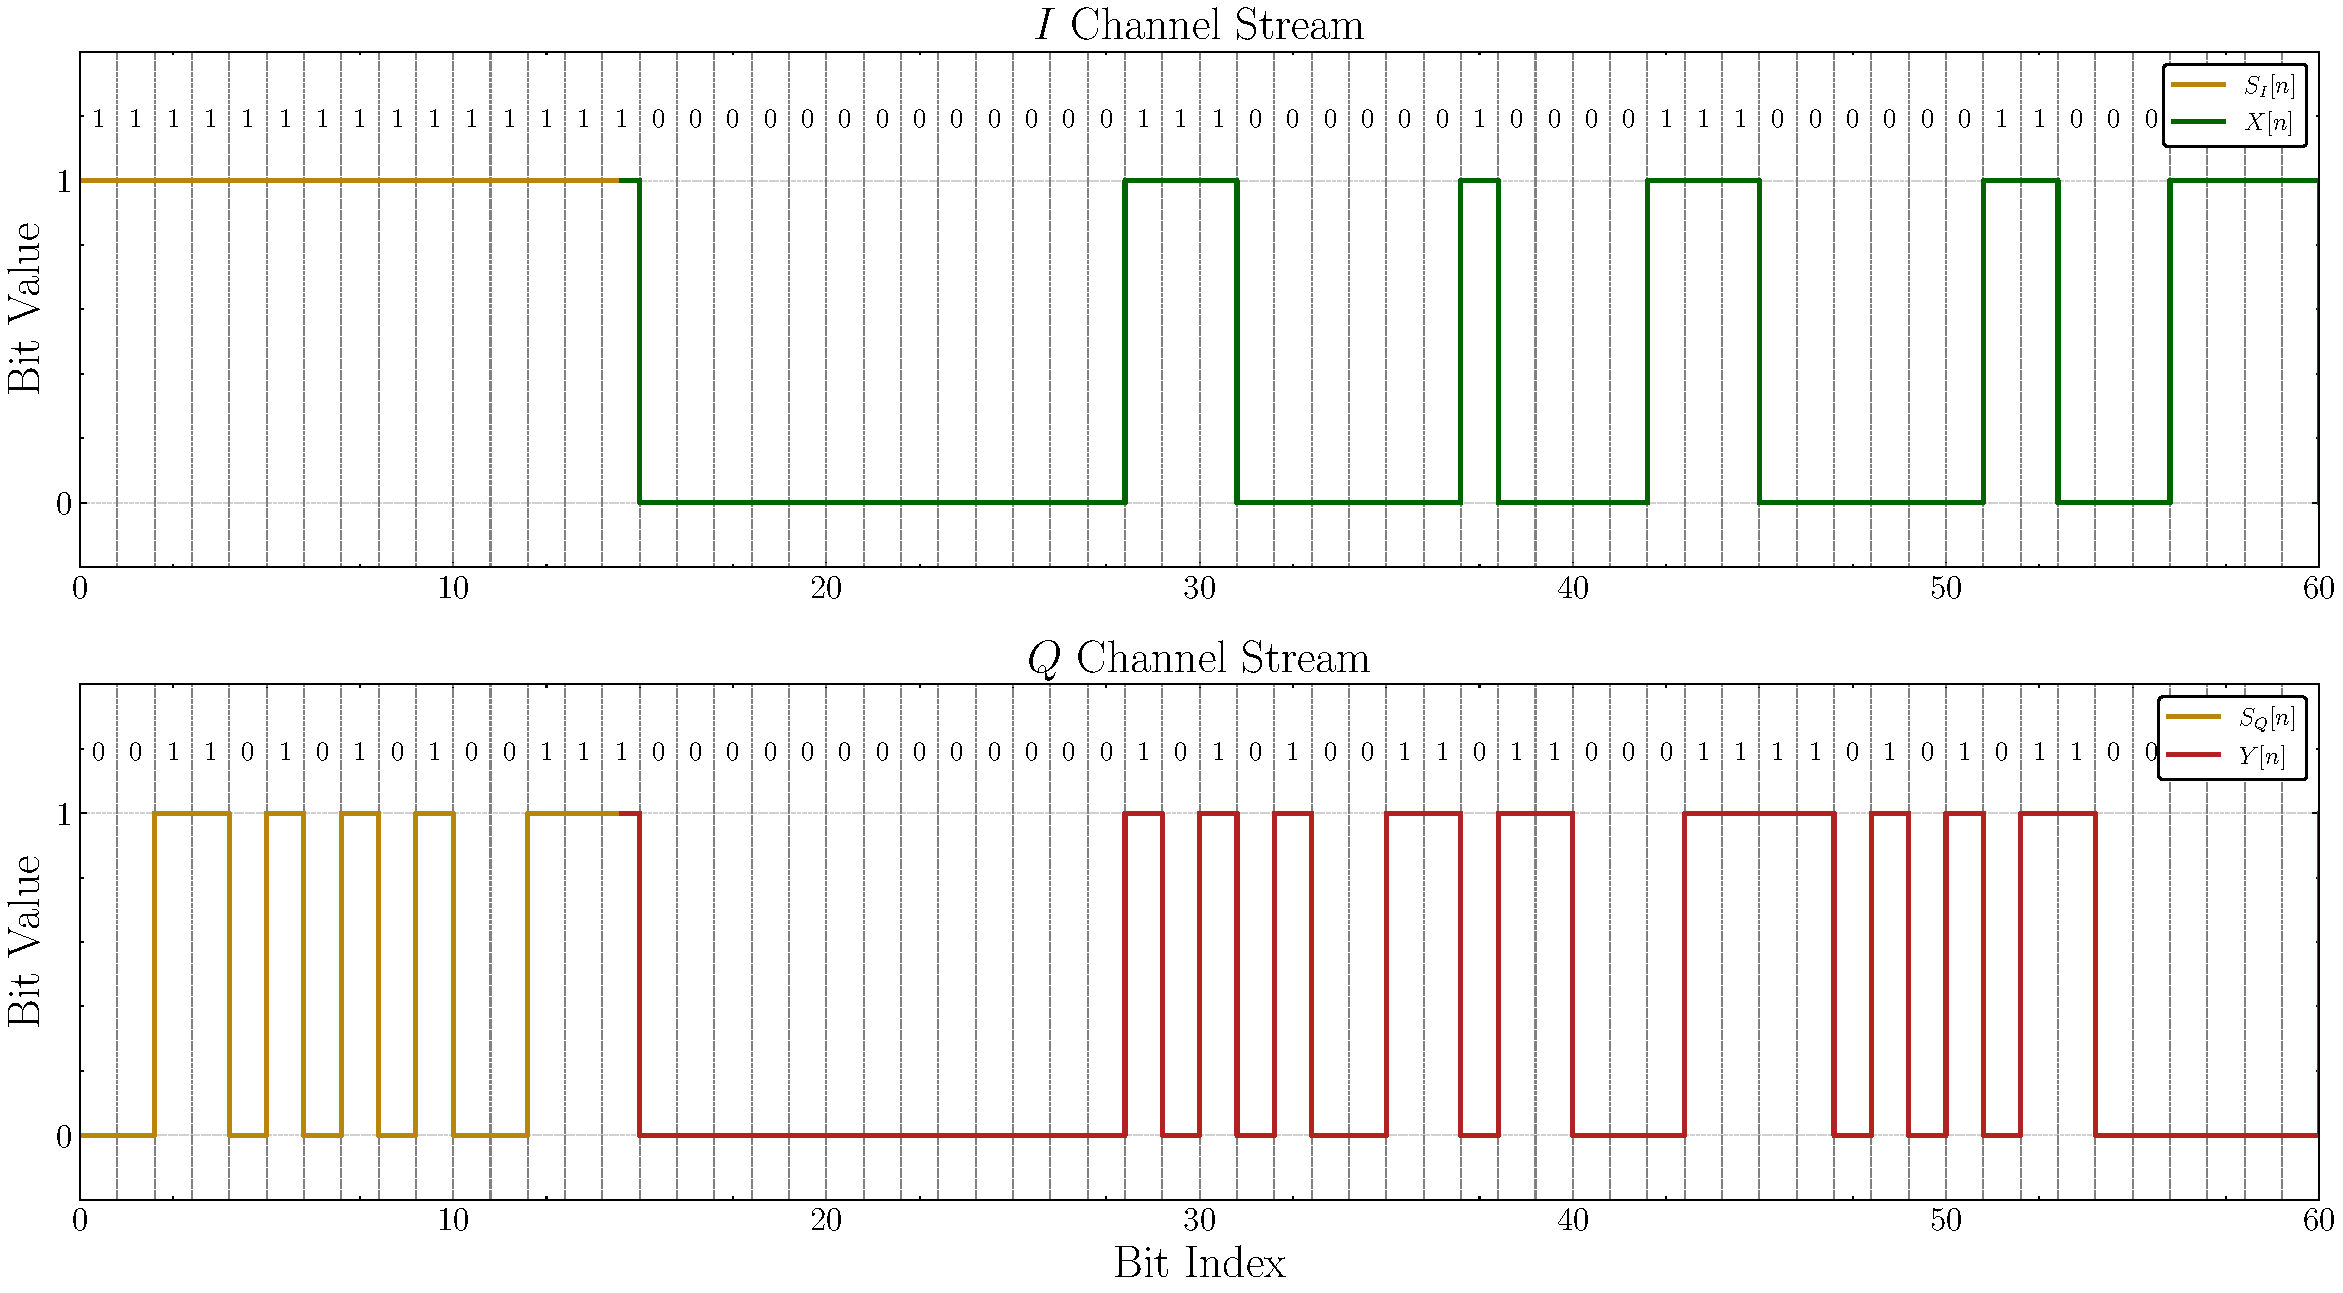
\includegraphics[width=\linewidth]{assets/cap3/transmitter_mux_time.pdf}
\end{figure}

Em seguida, os bits são codificados utilizando codificação de linha para melhorar as características espectrais do sinal modulado, como detalhado na seção \ref{sec:line_coding}, neste processo é utilizado apenas codificação \gls{NRZ} para os dois canais, pois a técnica \gls{Manchester} será aplicada posteriormente na modulação de pulso do canal \gls{cQ}, o processo de codificação de linha de ambos os canais é ilustrado na \autoref{fig:encoder_time}.

\begin{figure}[H]
	\centering
	\caption{Codificação de linha}\label{fig:encoder_time}
	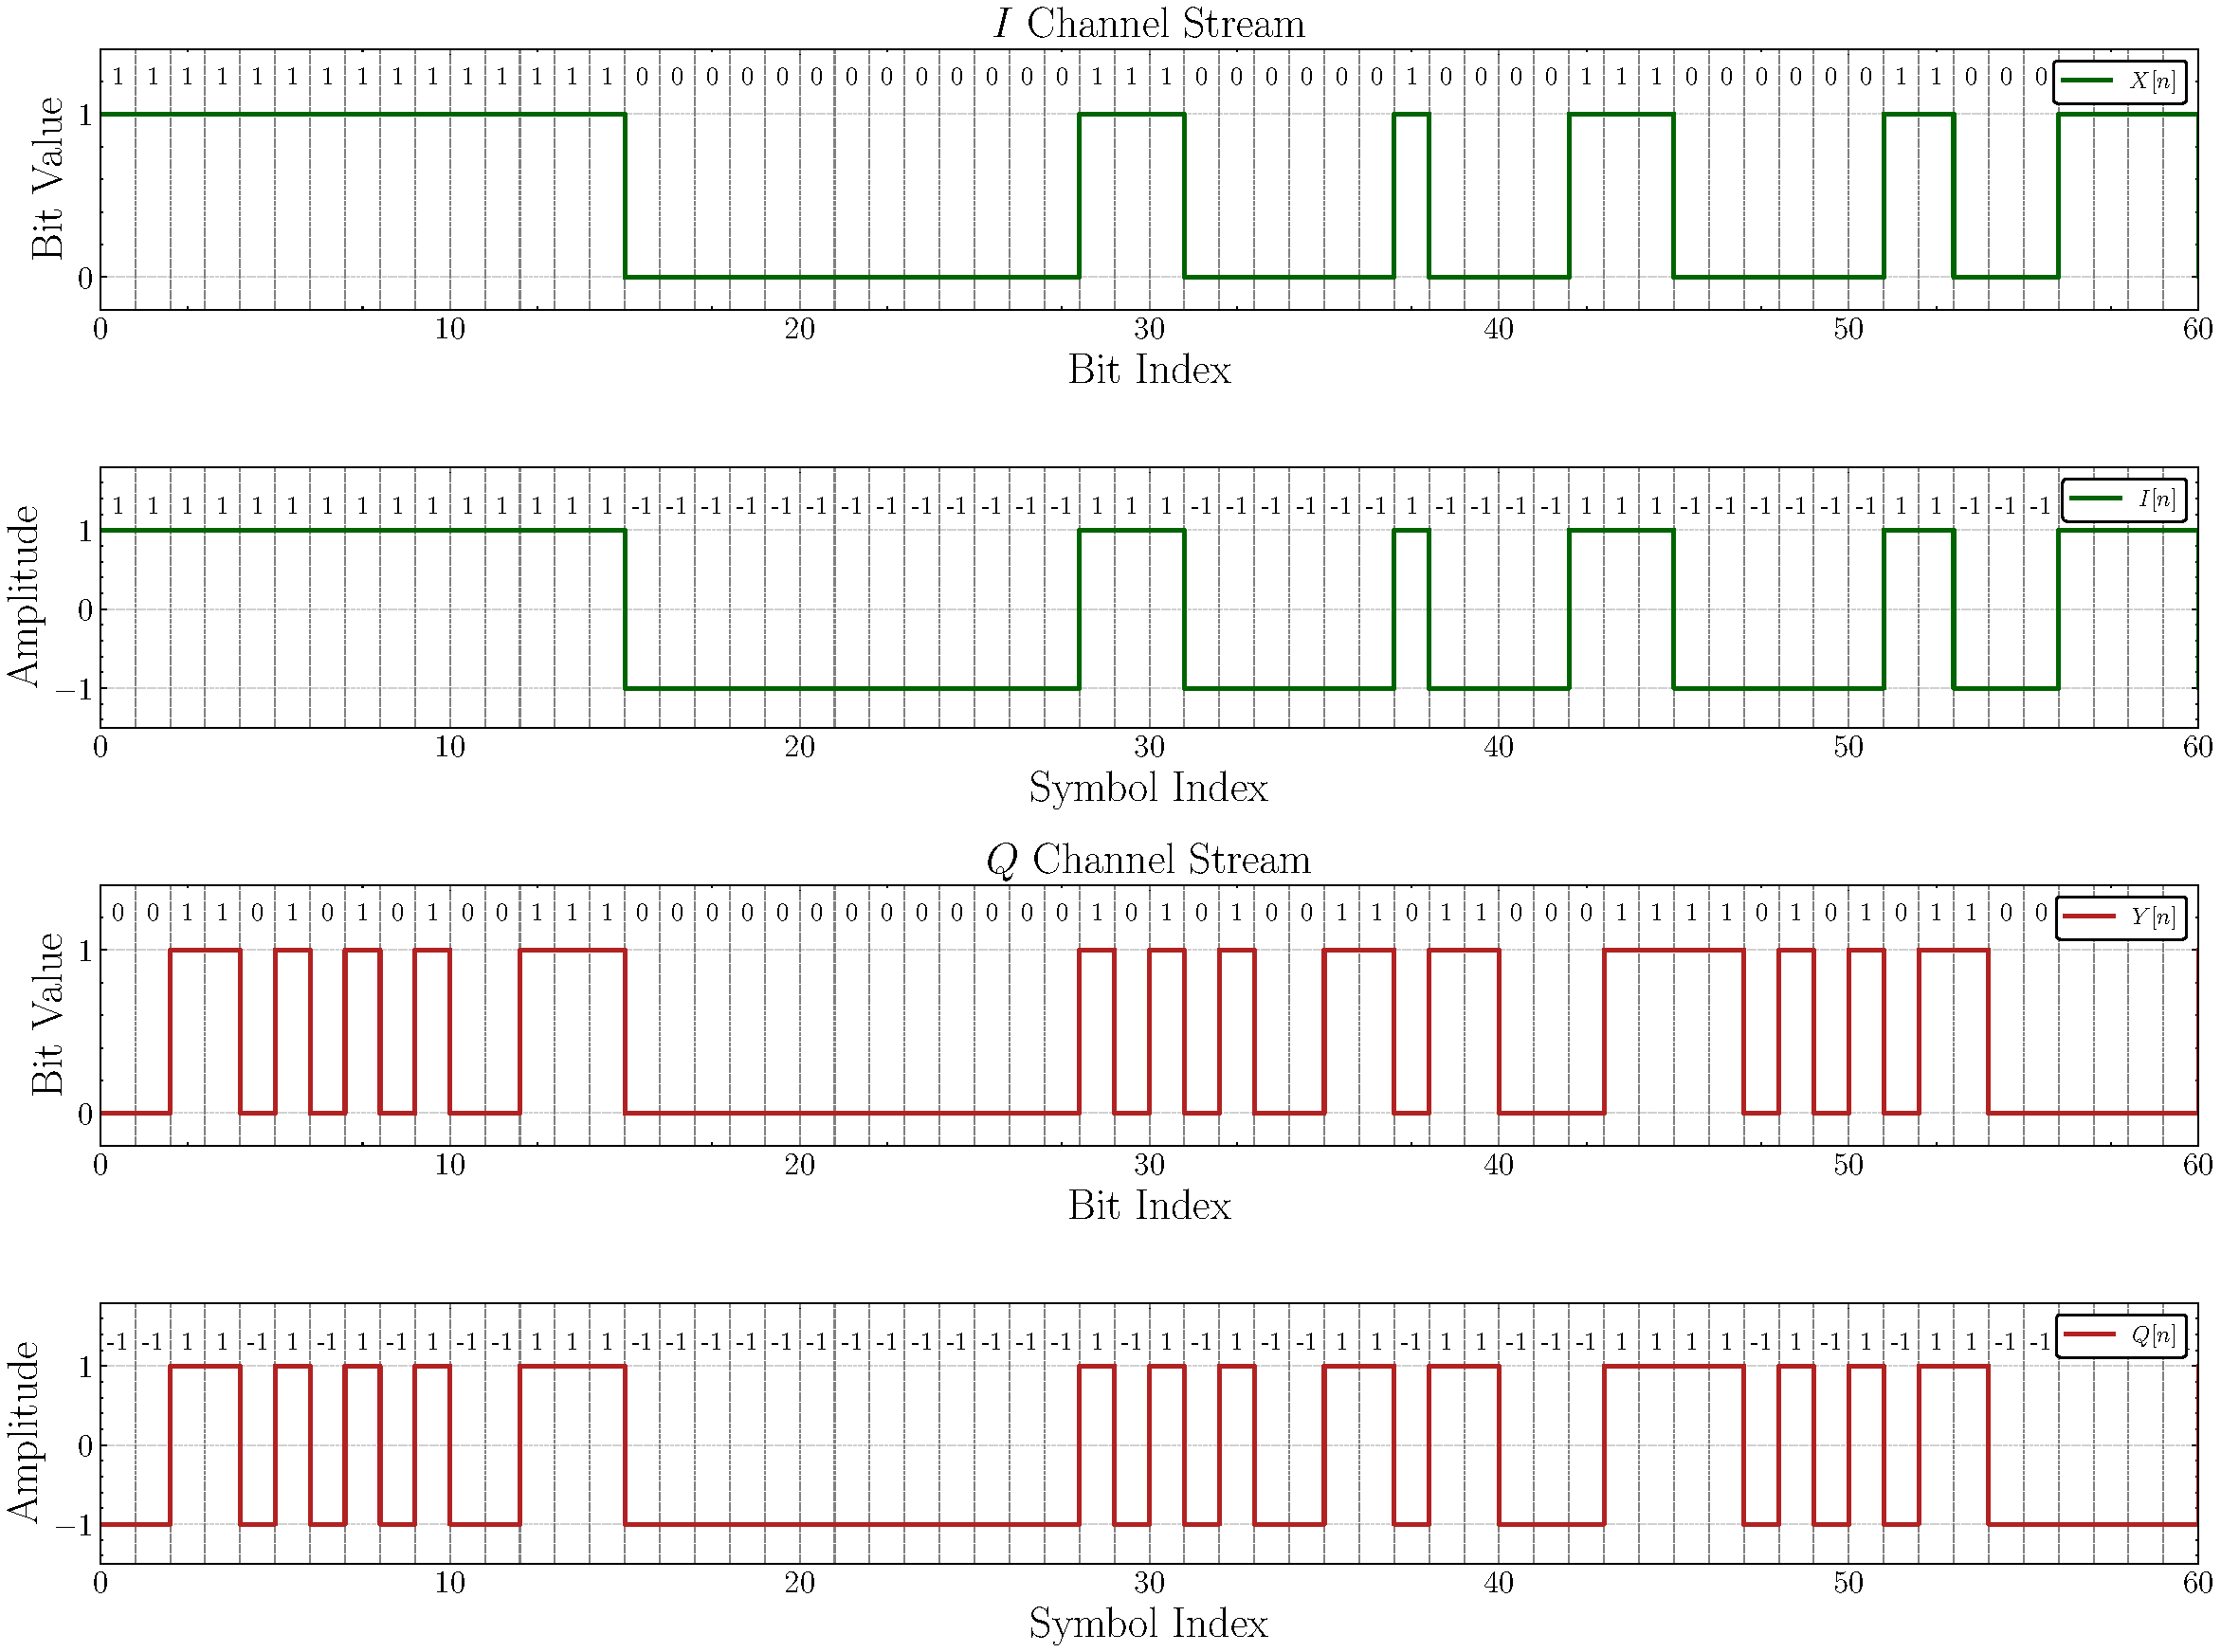
\includegraphics[width=\linewidth]{assets/cap3/transmitter_encoder_time.pdf}
\end{figure}

As sequências de simbolos \gls{In} e \gls{Qn} resultantes da codificação de linha, estão prontas para serem moduladas utilizando modulação de pulso. 

\subsection{Modulação de pulso RRC e Manchester}

Após a montagem das sequências de simbolos \gls{In} e \gls{Qn}, o próximo passo é a modulação de pulso, onde o canal \gls{cI} utiliza um filtro de pulso \gls{RRC} e o canal \gls{cQ} utiliza um filtro de pulso \gls{Manchester}, conforme detalhado na seção \ref{sec:line_coding}. A modulação de pulso é fundamental para reduzir a largura de banda \gls{W} do sinal que está sendo transmitido e também reduzir a interferência entre símbolos \gls{ISI}. O processo de modulação de pulso dos canais \gls{cI} e \gls{cQ} é ilustrado na \autoref{fig:pulse_modulate_diagram}.

\begin{figure}[H]
    \centering
    \caption{Diagrama de blocos do modulador de pulso para os canais $I$ e $Q$}\label{fig:pulse_modulate_diagram}
    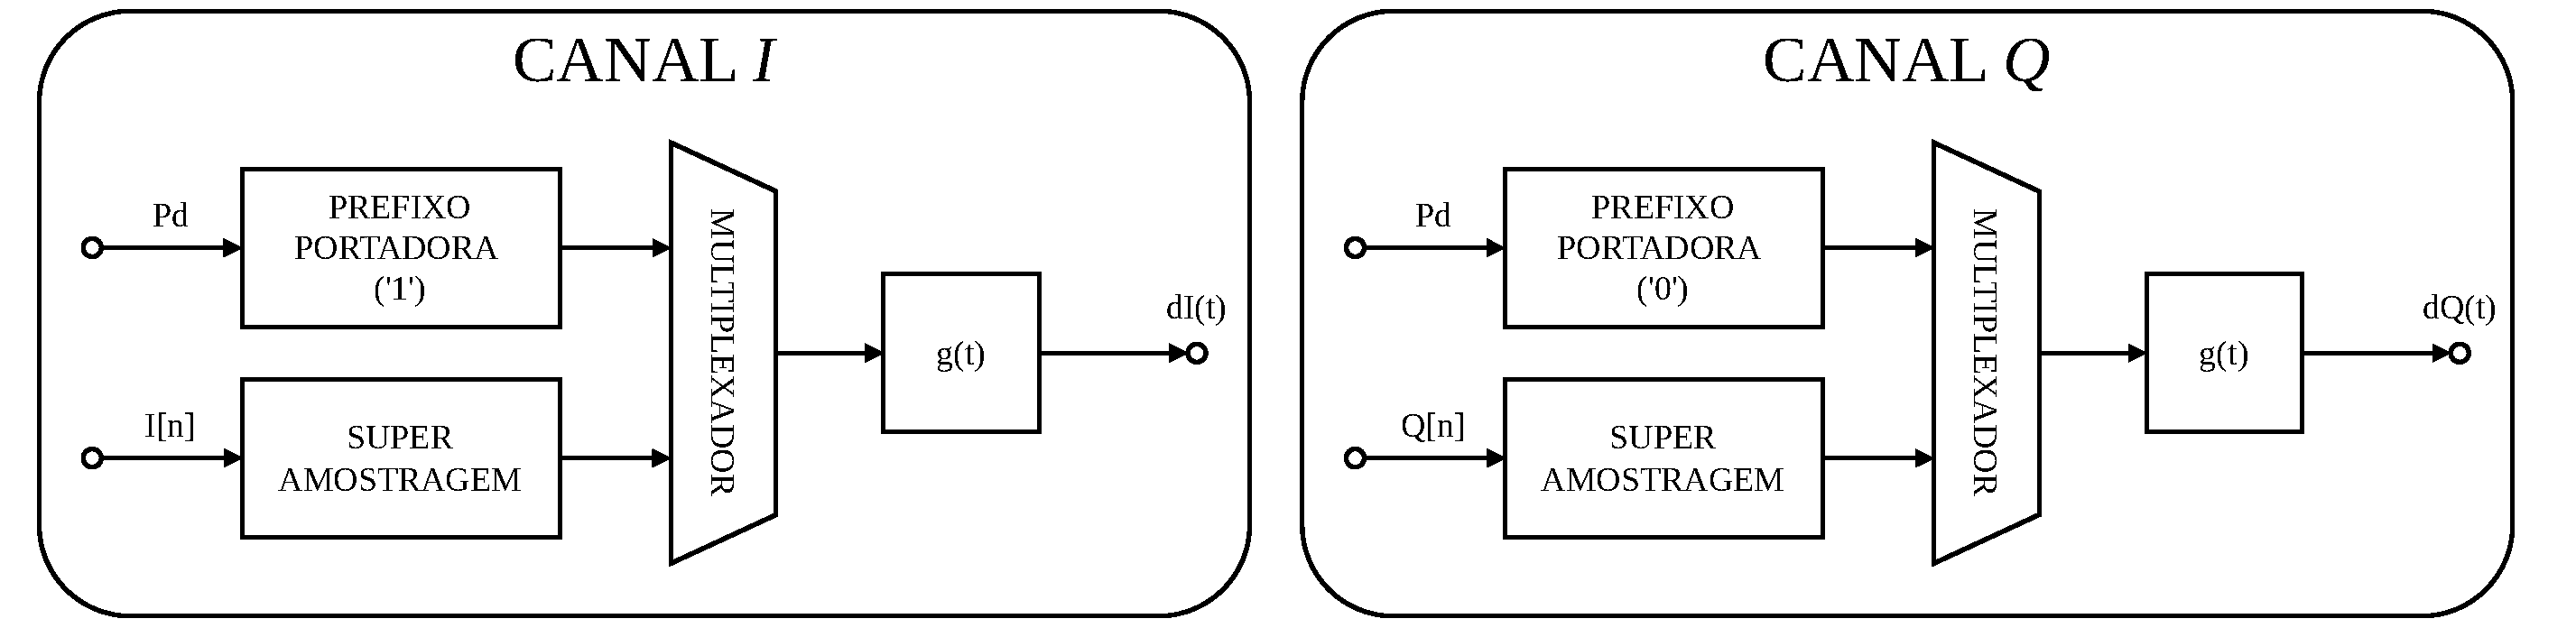
\includegraphics[width=\linewidth]{assets/diagrams/pulse_modulate.pdf}
\end{figure}

\subsubsection{Pulso RRC e Manchester}

Antes de aplicar a modulação de pulso, é necessário gerar os filtros de pulso \gls{RRC} e \gls{Manchester}, que serão utilizados para modular os canais \gls{cI} e \gls{cQ}, respectivamente. A resposta ao impulso do filtro \gls{RRC} é ilustrada na \autoref{fig:impulse_response_rrc}, e é calculada conforme apresentado na seção \ref{sec:pulse_modulation}. 

\begin{figure}[H]
	\centering
	\caption{Resposta ao impulso - Pulso RRC}\label{fig:impulse_response_rrc}
	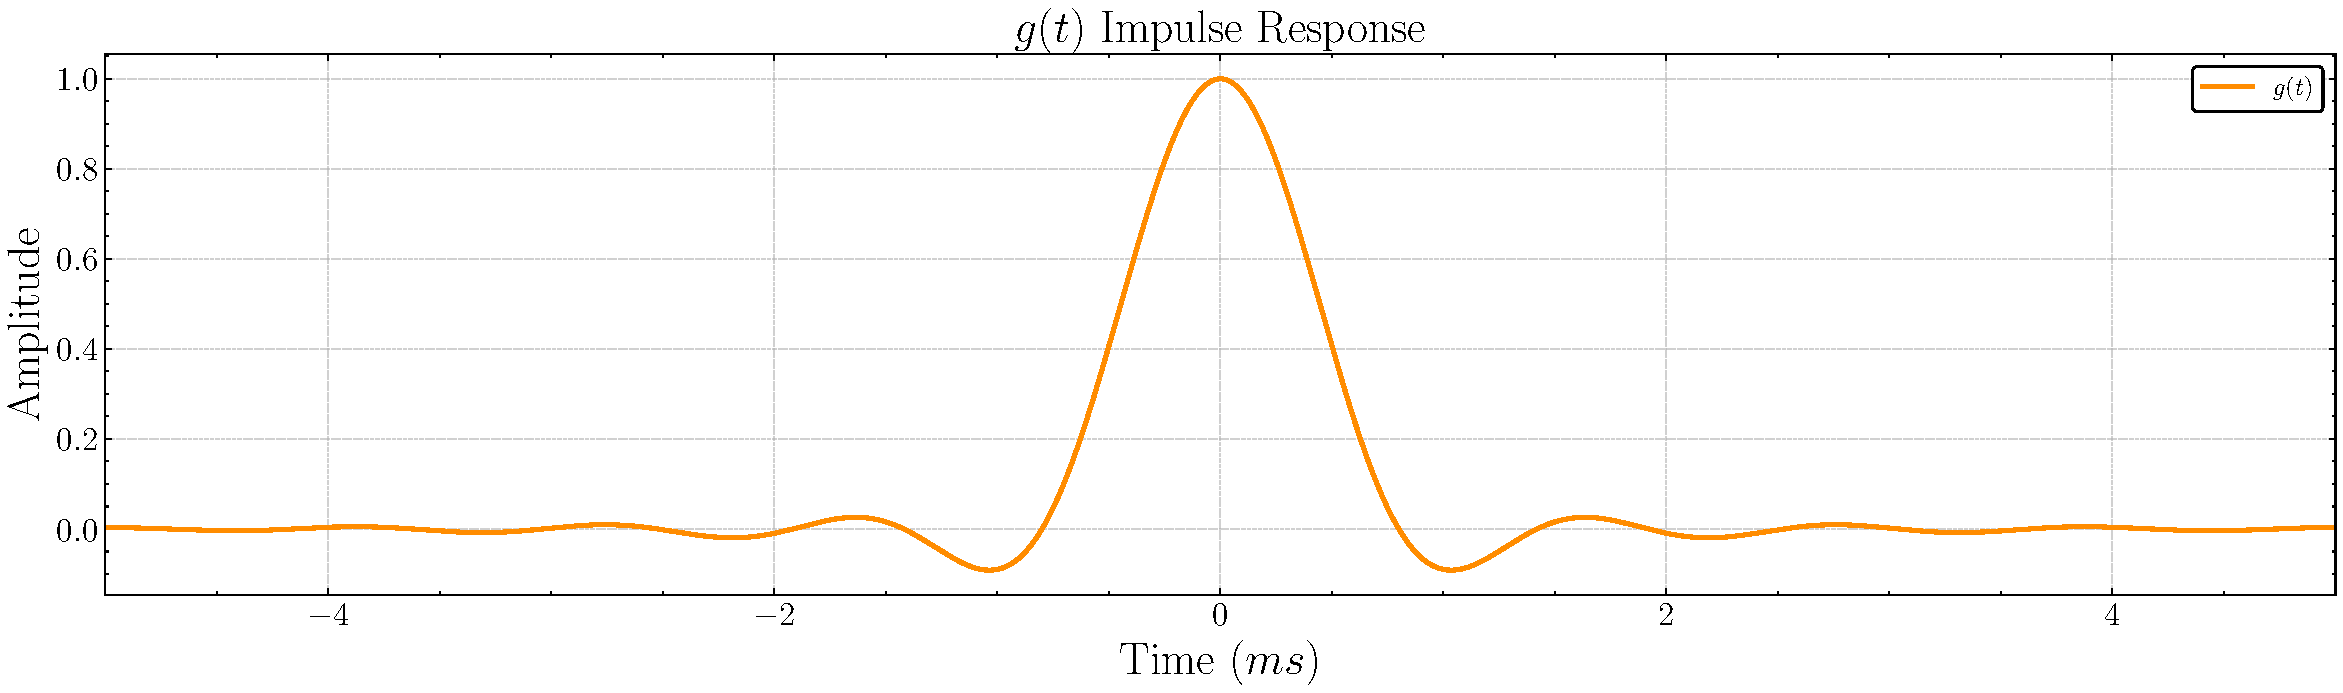
\includegraphics[width=\linewidth]{assets/cap3/example_formatter_impulse.pdf}
\end{figure}

Já o pulso \gls{Manchester} é gerado através de uma soma de dois pulsos \gls{RRC} deslocados no tempo, um positivo deslocado em $T_b/2$ e outro negativo deslocado em $-T_b/2$, conforme ilustrado na \autoref{fig:impulse_response_man}. O calculo do pulso pode ser expresso como 

\begin{equation}
g_{MAN}(t) = g_{RRC}(t + T_b/2) - g_{RRC}(t - T_b/2)
\end{equation}

Onde $g_{MAN}(t)$ é o pulso Manchester, $g_{RRC}(t)$ é o pulso RRC e $T_b$ é o tempo de bit. A resposta ao impulso do filtro \gls{Manchester} é ilustrada na \autoref{fig:impulse_response_man}.

\begin{figure}[H]
	\centering
	\caption{Resposta ao impulso - Pulso Manchester}\label{fig:impulse_response_man}
	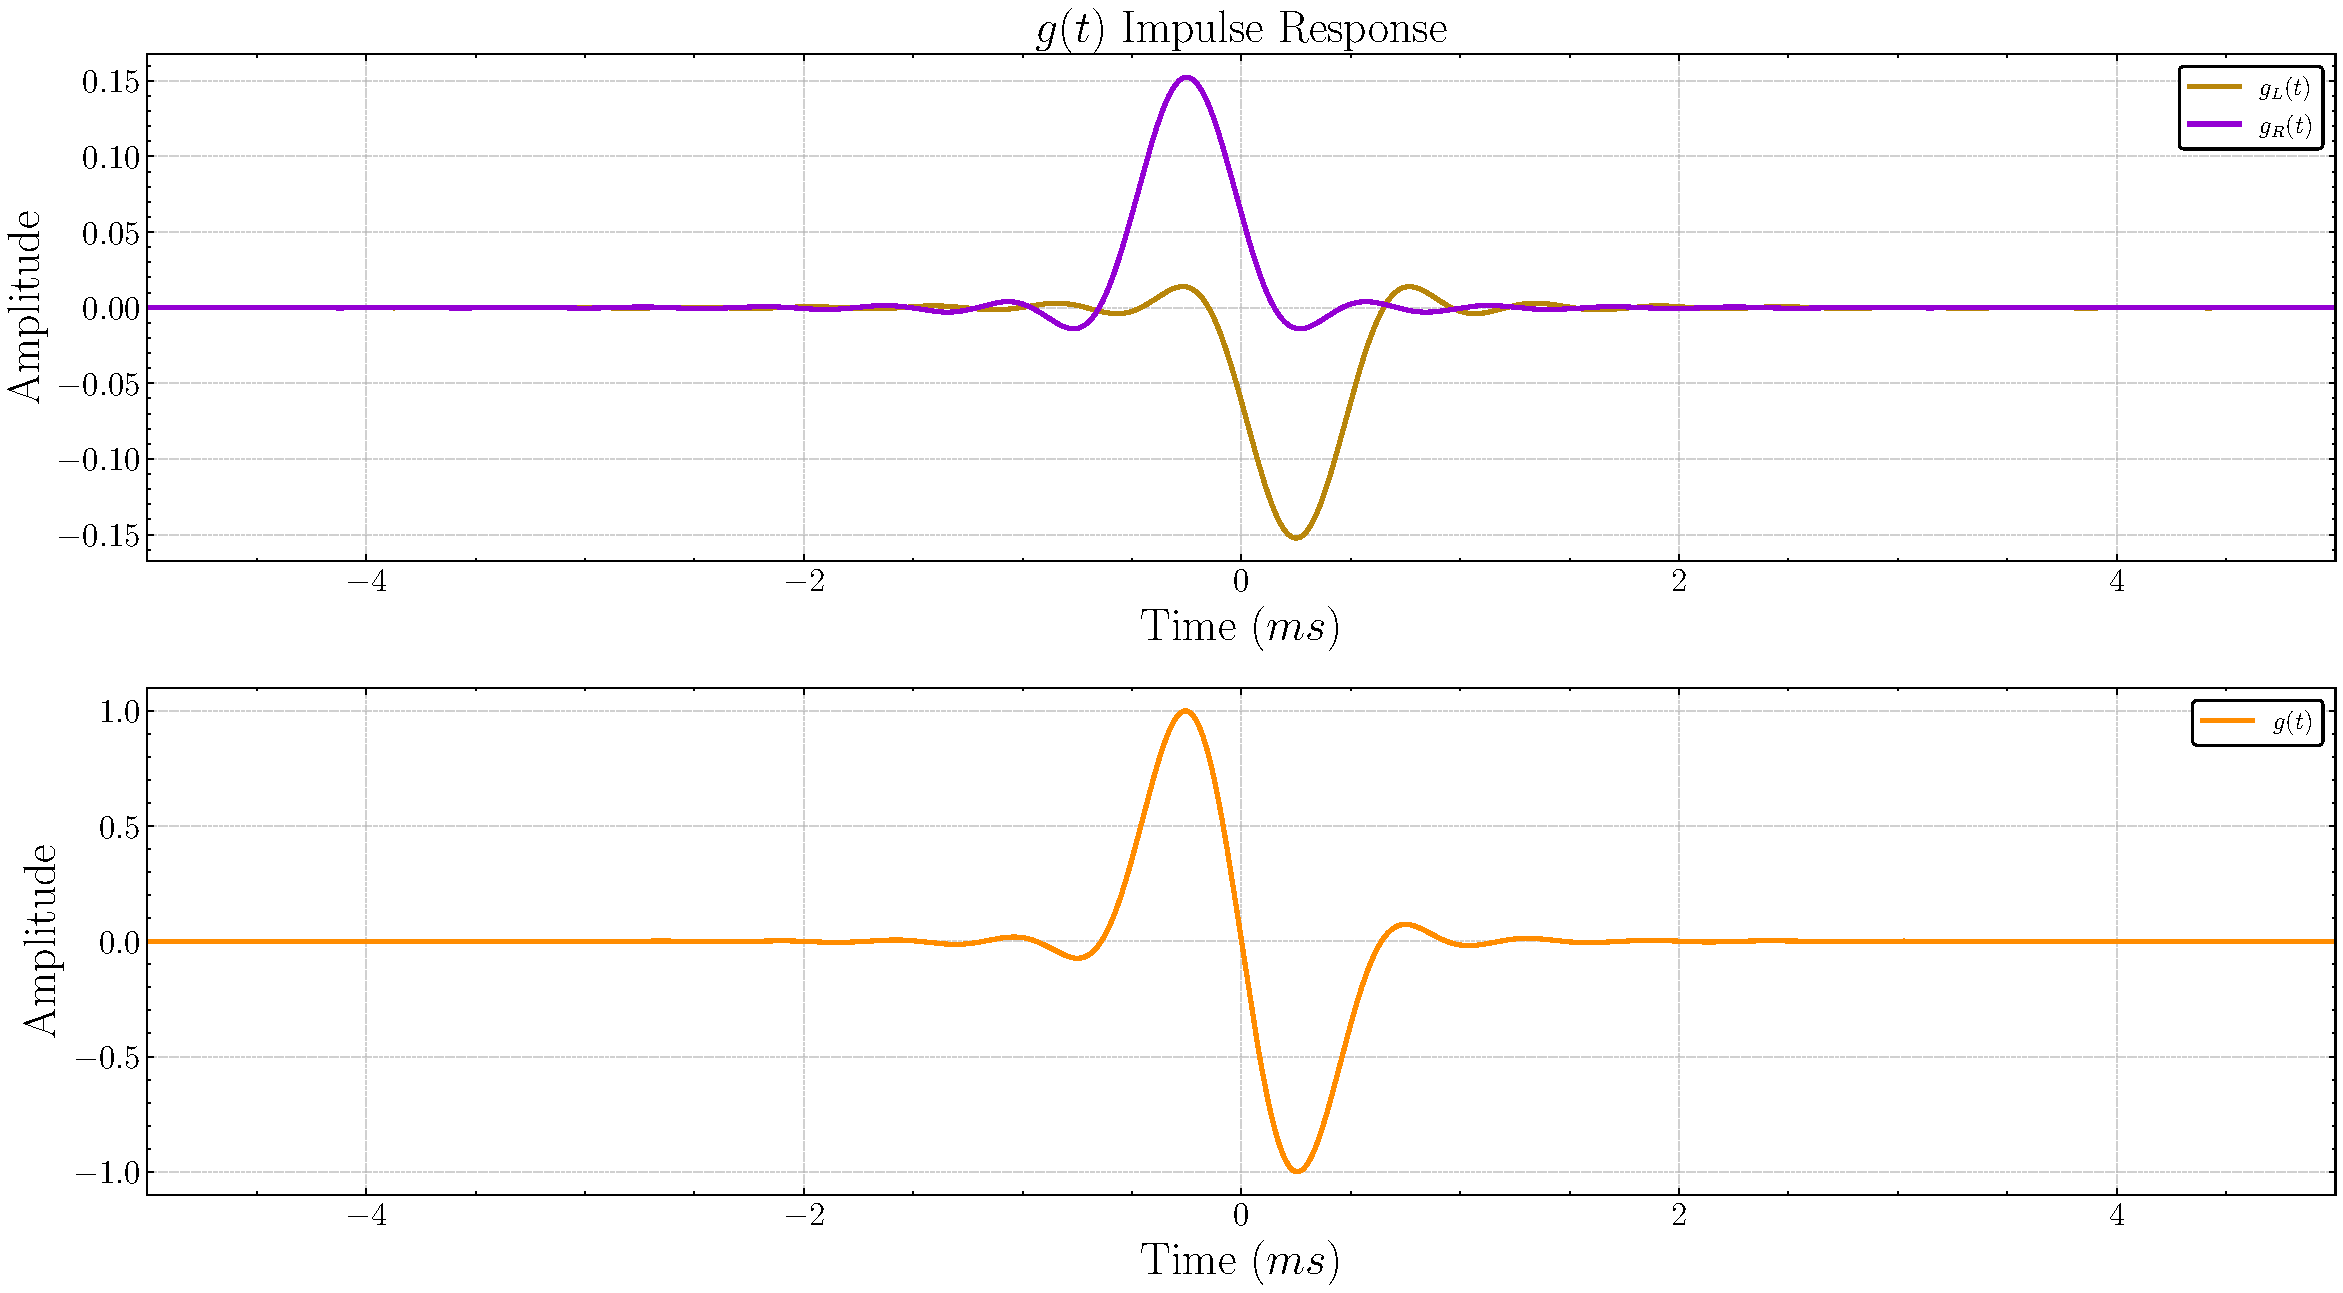
\includegraphics[width=\linewidth]{assets/cap3/example_formatter_impulse_man.pdf}
\end{figure}

A utilização do pulso \gls{Manchester} no canal \gls{cQ} ao invés da codificação de linha \gls{Manchester} proposta originalmente tem como objetivo simplificar a implementação do sistema, reduzindo a complexidade computacional e o número de etapas necessárias na cadeia de transmissão. 

\subsubsection{Modulação de pulso dos canais I e Q}

Uma vez com os filtros de pulso \gls{RRC} e \gls{Manchester} gerados, é possível aplicar a modulação de pulso nos canais \gls{cI} e \gls{cQ}, respectivamente gerando os sinais \gls{dI} e \gls{dQ} modulados em banda base. Esse processo envolve a superamostragem dos vetores de simbolos \gls{In} e \gls{Qn}, em função da frequência de amostragem \gls{fs}, seguida da filtragem com os respectivos filtros de pulso. 

O resultado são as sequências \gls{dI} e \gls{dQ} contínuas ao longo do tempo \gls{t}, onde cada bit de informação é transmitido durante um período de tempo $\text{ \gls{Tb}} = 1/ \text{\gls{Rb}}$ (tempo de bit), definido com base na taxa de bit \gls{Rb}. A modulação de pulso dos canais \gls{cI} e \gls{cQ} é ilustrada na \autoref{fig:transmitter_formatter_time}.

\begin{figure}[H]
	\centering
	\caption{Modulação de pulso dos canais $I$ e $Q$}\label{fig:transmitter_formatter_time}
	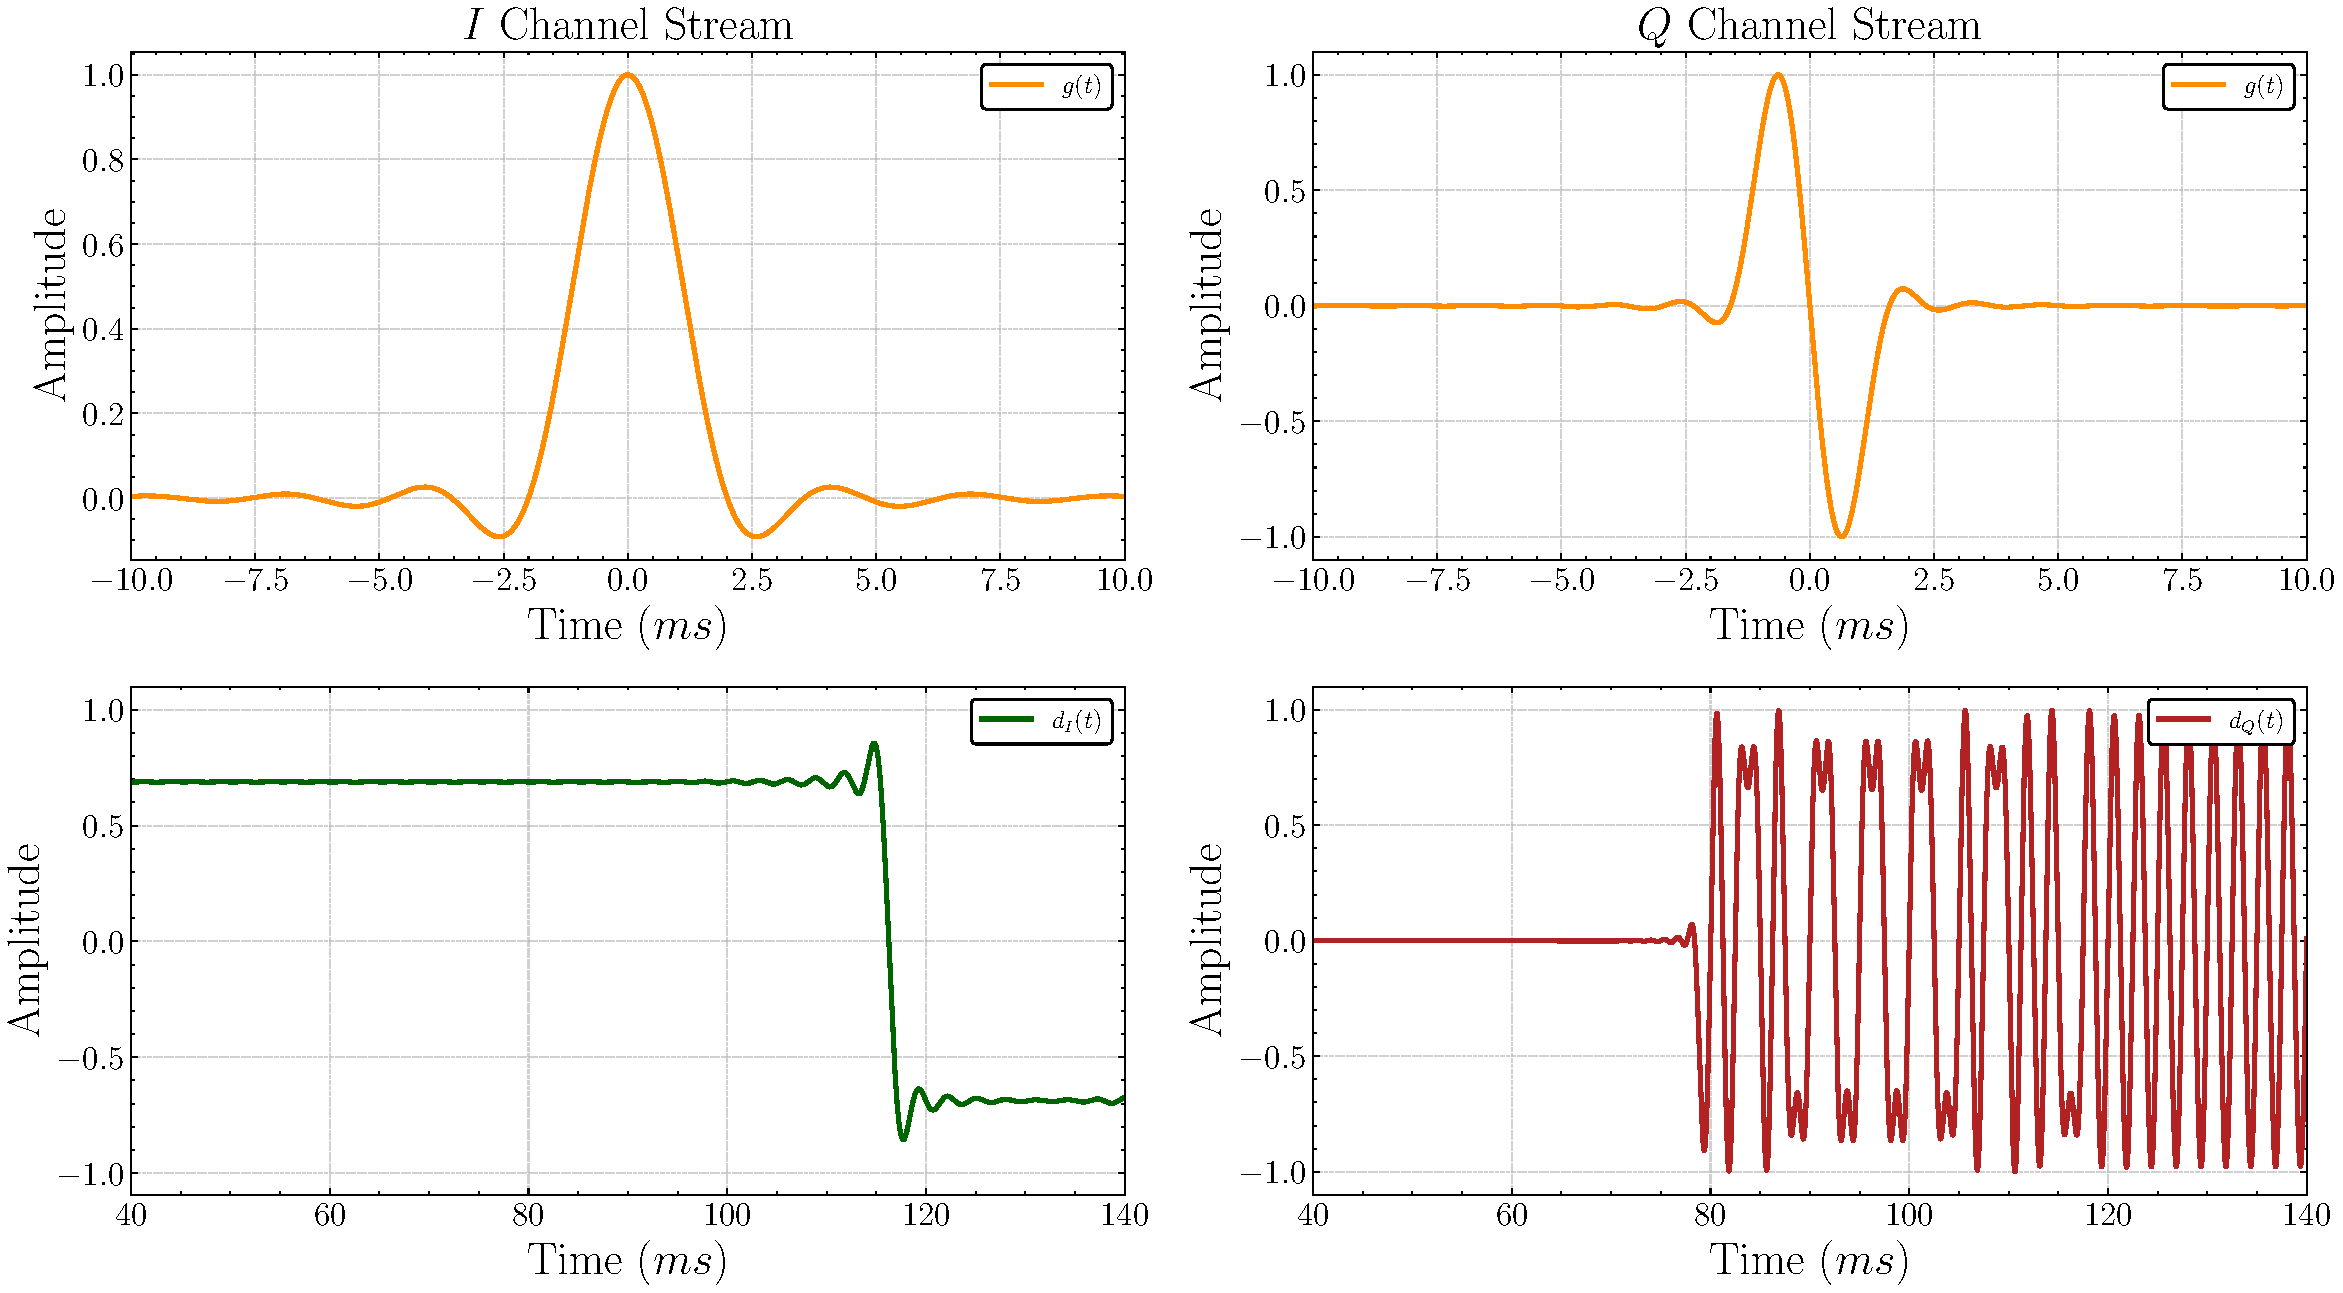
\includegraphics[width=\linewidth]{assets/cap3/transmitter_formatter_time.pdf}
\end{figure}

As sequências \gls{dI} e \gls{dQ} estão agora prontas para serem moduladas em banda passante utilizando modulação em fase em quadratura (\gls{QPSK}), conforme detalhado na seção \ref{sec:qpsk}.

\subsection{Modulação em fase em quadratura (QPSK)}\label{sec:qpsk}

Na modulação \gls{QPSK}, os sinais modulados em banda base \gls{dI} e \gls{dQ} são utilizados para modular uma componente senoideal e uma componente cossenoidal, respectivamente, com frequência \gls{fc}, o somatório dessas duas componentes moduladas resulta no sinal modulado em banda passante \gls{st}, conforme ilustrado na \autoref{fig:transmitter_modulator_time}.

\begin{figure}[H]
	\centering
	\caption{Modulação em banda passante canais $I$ e $Q$}\label{fig:transmitter_modulator_time}
	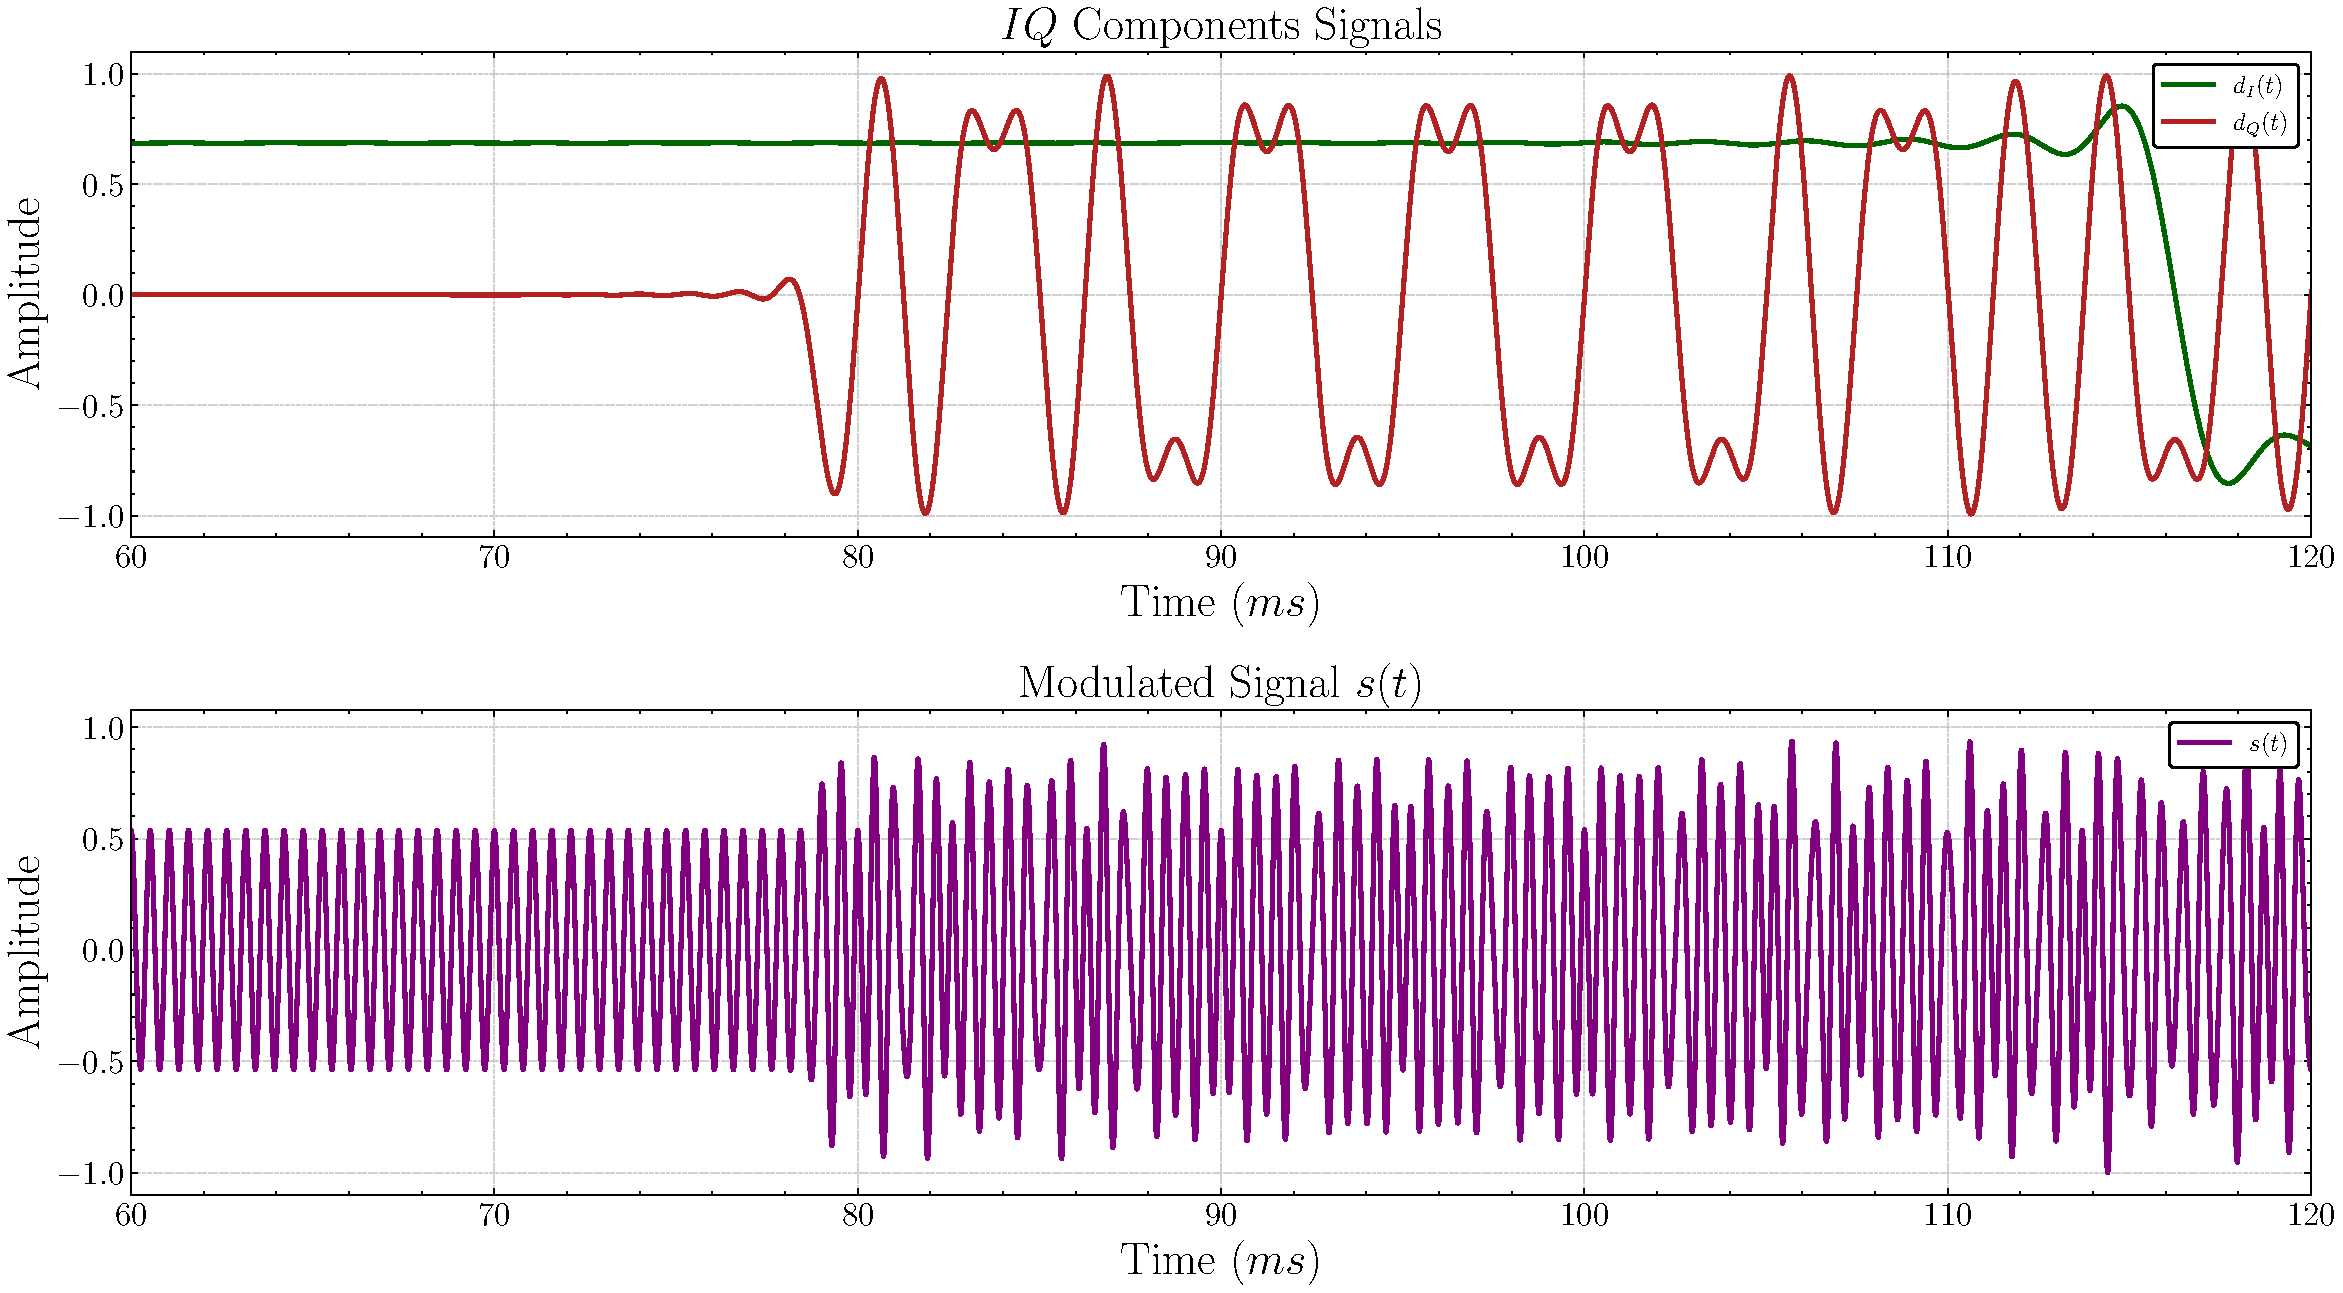
\includegraphics[width=\linewidth]{assets/cap3/transmitter_modulator_time.pdf}
\end{figure}

A partir do sinal modulado \gls{st}, é possível observar a constelação do sinal \gls{QPSK}, isto é o comportamento do sinal \gls{st} no \gls{iqplane}, que idealmente para o \gls{QPSK} é composto por quatro pontos distintos, cada um representando uma combinação única dos bits transmitidos pelos canais \gls{cI} e \gls{cQ}. A constelação do sinal modulado \gls{st} é ilustrada na \autoref{fig:transmitter_modulator_constellation}, onde é possível observar a fase do sinal modulado e a constelação resultante no \gls{iqplane}.


\begin{figure}[H]
	\centering
	\caption{Fase e Constelação do sinal modulado $s(t)$}\label{fig:transmitter_modulator_constellation}
	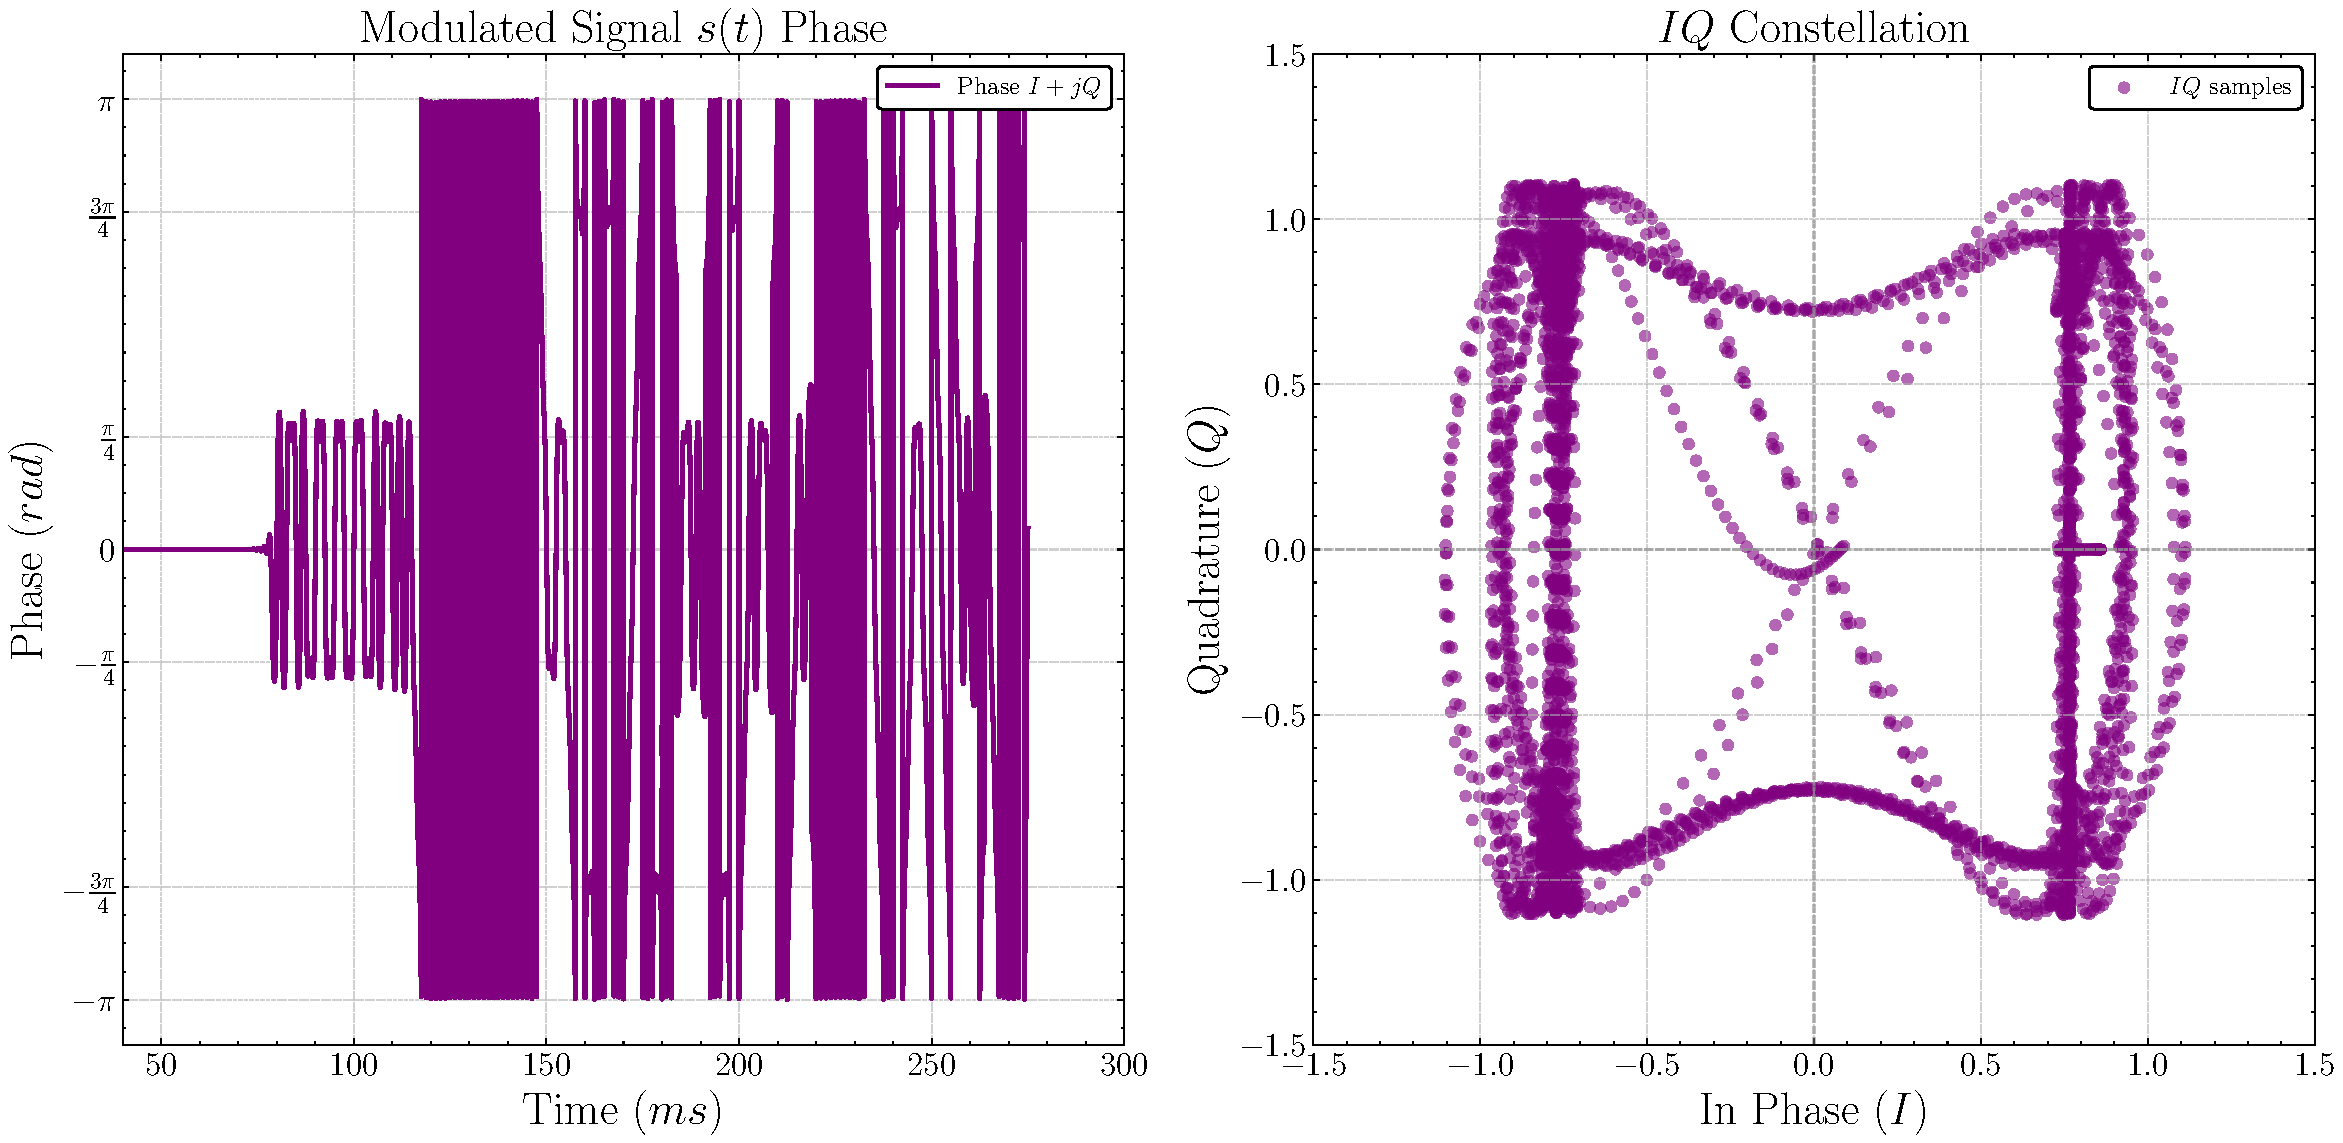
\includegraphics[width=\linewidth]{assets/cap3/transmitter_modulator_constellation.pdf}
\end{figure}


\subsubsection{Adição de portadora pura}

Ao se observar mais atentamente a \ref{fig:transmitter_modulator_time} e também \ref{fig:transmitter_formatter_time} pode-se notar que no inicio da transmissão, a componente \gls{dI} está com amplitude estável e proxima á $`1`$, enquanto que a componente \gls{dQ} está estável com amplitude igual a $`0`$, essa é configuração é proposital dentro do \gls{Pd} para que a sequência resultante modulada em banda passante tenha um periodo de fase estável, ou seja, uma portadora pura, antes do inicio da transmissão dos dados. O equacionamento para o período de portadora pura pode ser expresso como

\begin{equation}
    s(t) = 1(t) \cdot \cos(2\pi f_c t) - 0(t) \cdot \sin(2\pi f_c t) \mapsto s(t) = \cos(2\pi f_c t)
\end{equation}

\noindent Onde $1(t)$ é a componente \gls{dI} com valor constante $`1`$ e $0(t)$ é a componente \gls{dQ} com valor constante $`0`$. O período de portadora pura é fundamental para o receptor identificar a frequência da portadora \gls{fc} e realizar a detecção do sinal corretamente, conforme detalhado na seção \ref{sec:detector}. A duração do período de portadora pura é definida pelo parâmetro \gls{Pd}, que no padrão \gls{ARGOS-III} é aproximadamente $0.082$ segundos.

Com o sinal modulado em banda passante \gls{st} conforme definido acima, podemos também verificar a presença da portadora pura nos primeiros instantes da transmissão, isto é ilustrado na figura \ref{fig:transmitter_modulator_portadora} apresentada abaixo.

\begin{figure}[H]
	\centering
	\caption{Comparação de portadora pura e sinal modulado}\label{fig:transmitter_modulator_portadora}
	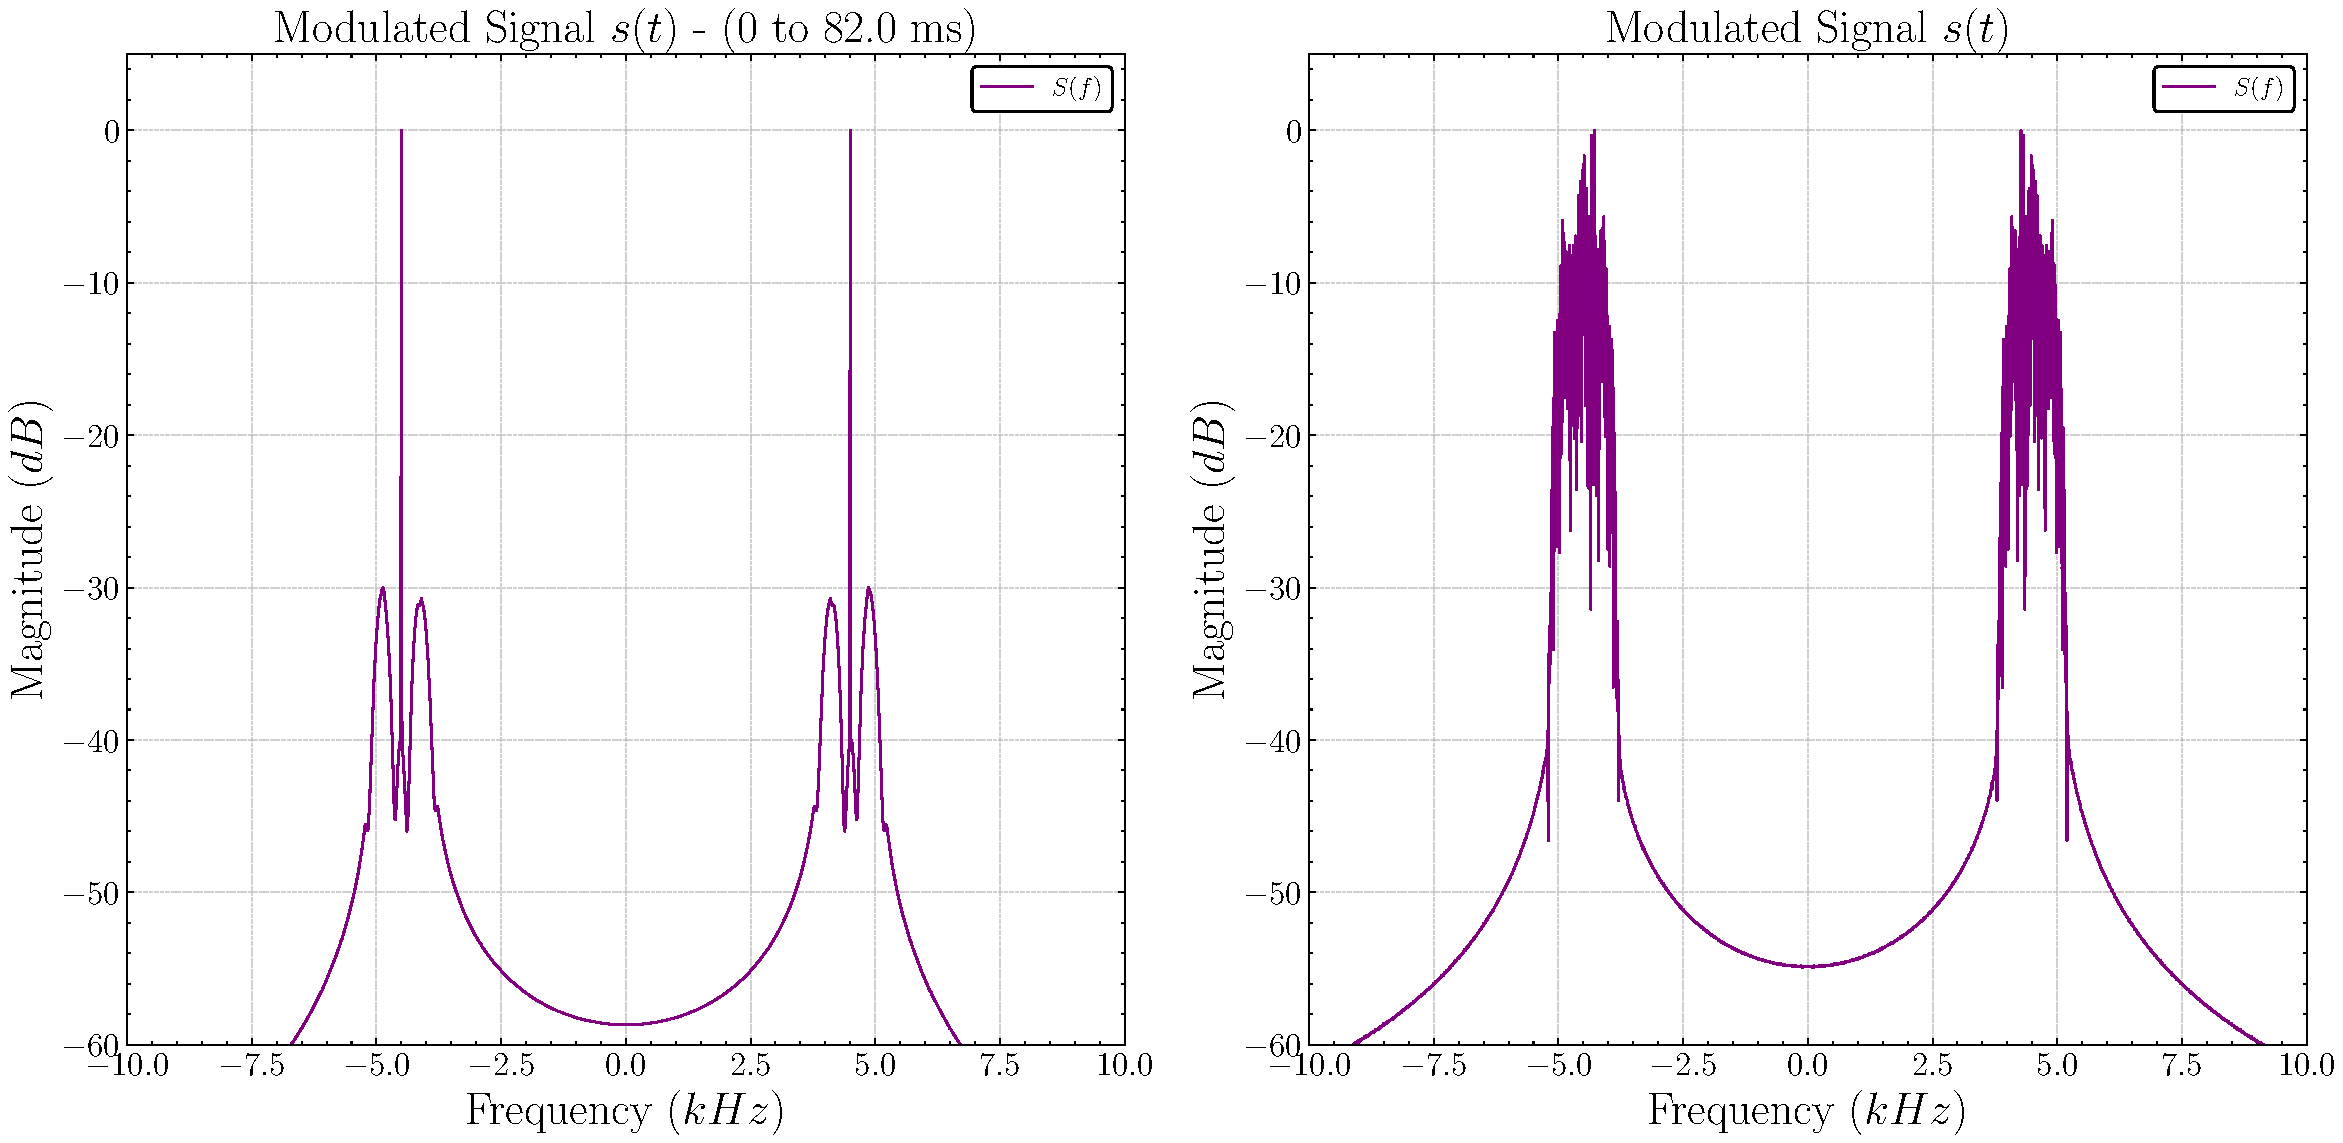
\includegraphics[width=\linewidth]{assets/cap3/transmitter_modulator_portadora.pdf}
\end{figure}

\section{CANAL E ADIÇÃO DE RUÍDO}\label{sec:canal}



\begin{figure}[H]
	\centering
	\caption{Diagrama de blocos do canal}\label{fig:channel_diagram}
	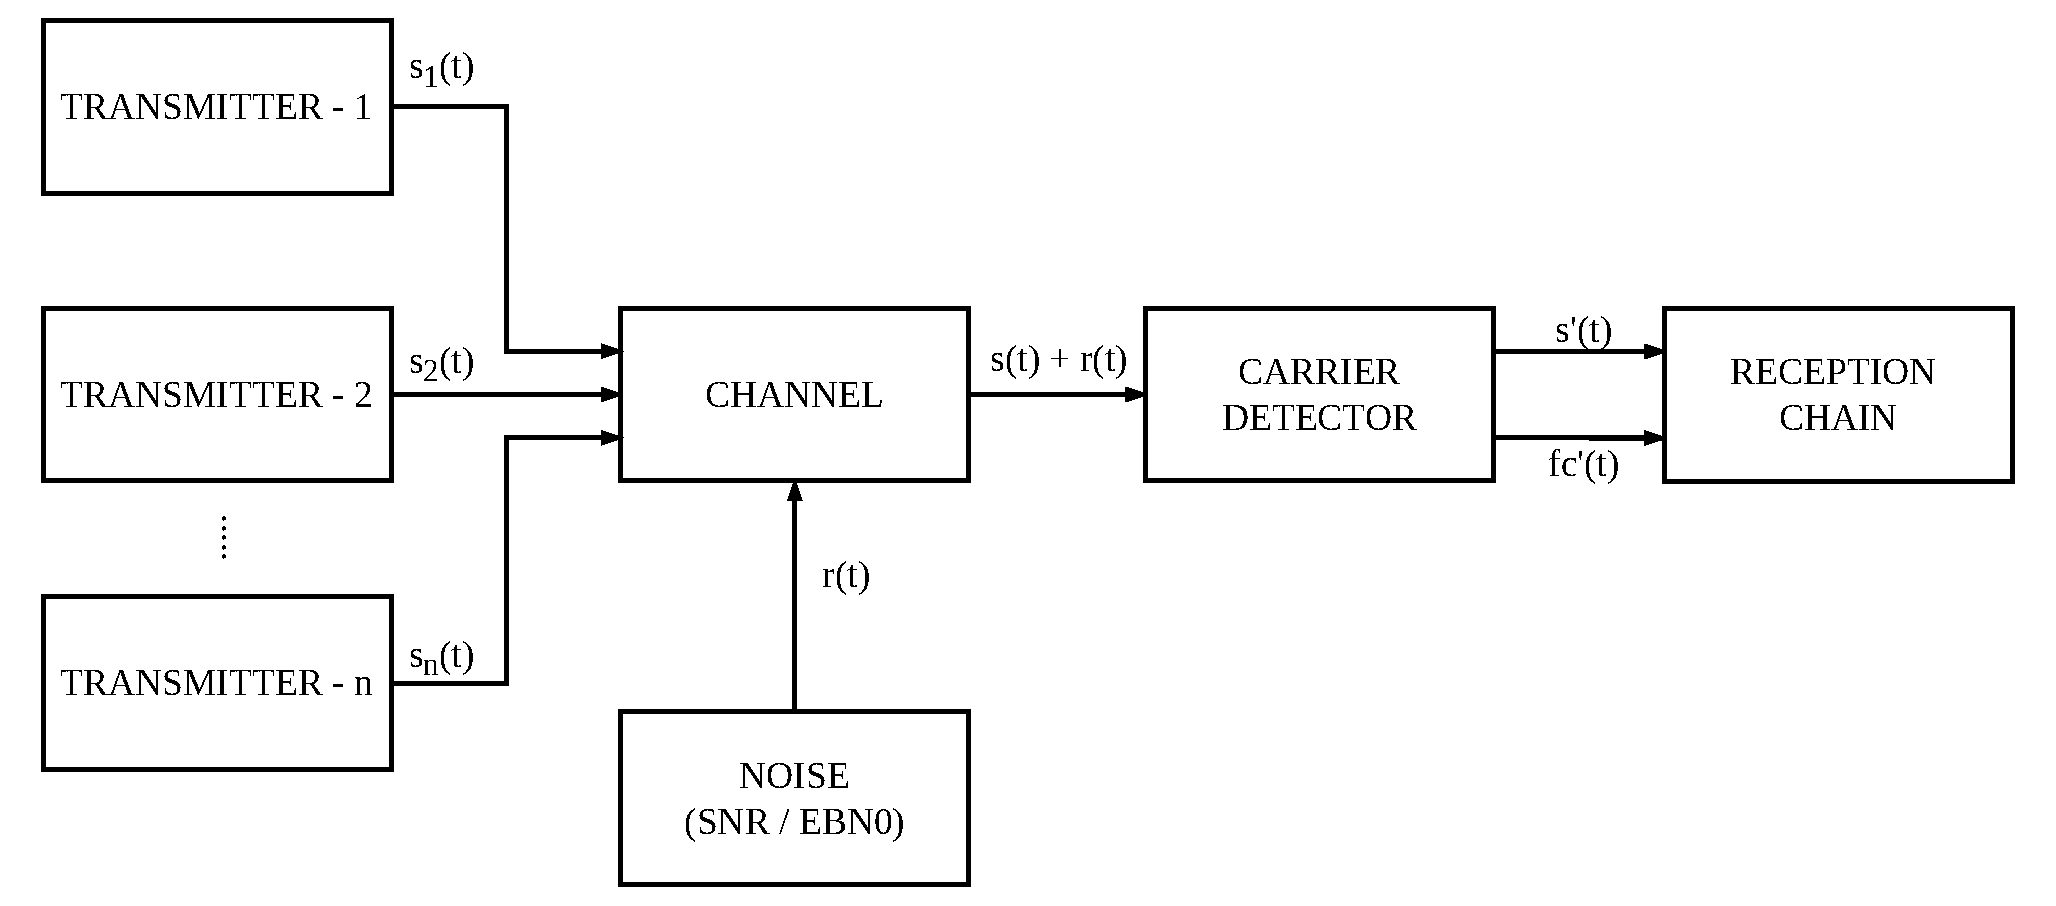
\includegraphics[width=\linewidth]{assets/diagrams/channel.pdf}
\end{figure}

\subsection{Modelo de canal}\label{sec:modelo_canal}

\begin{figure}[H]
	\centering
	\caption{Adição de multiplas transmissões no canal}\label{fig:channel_time}
	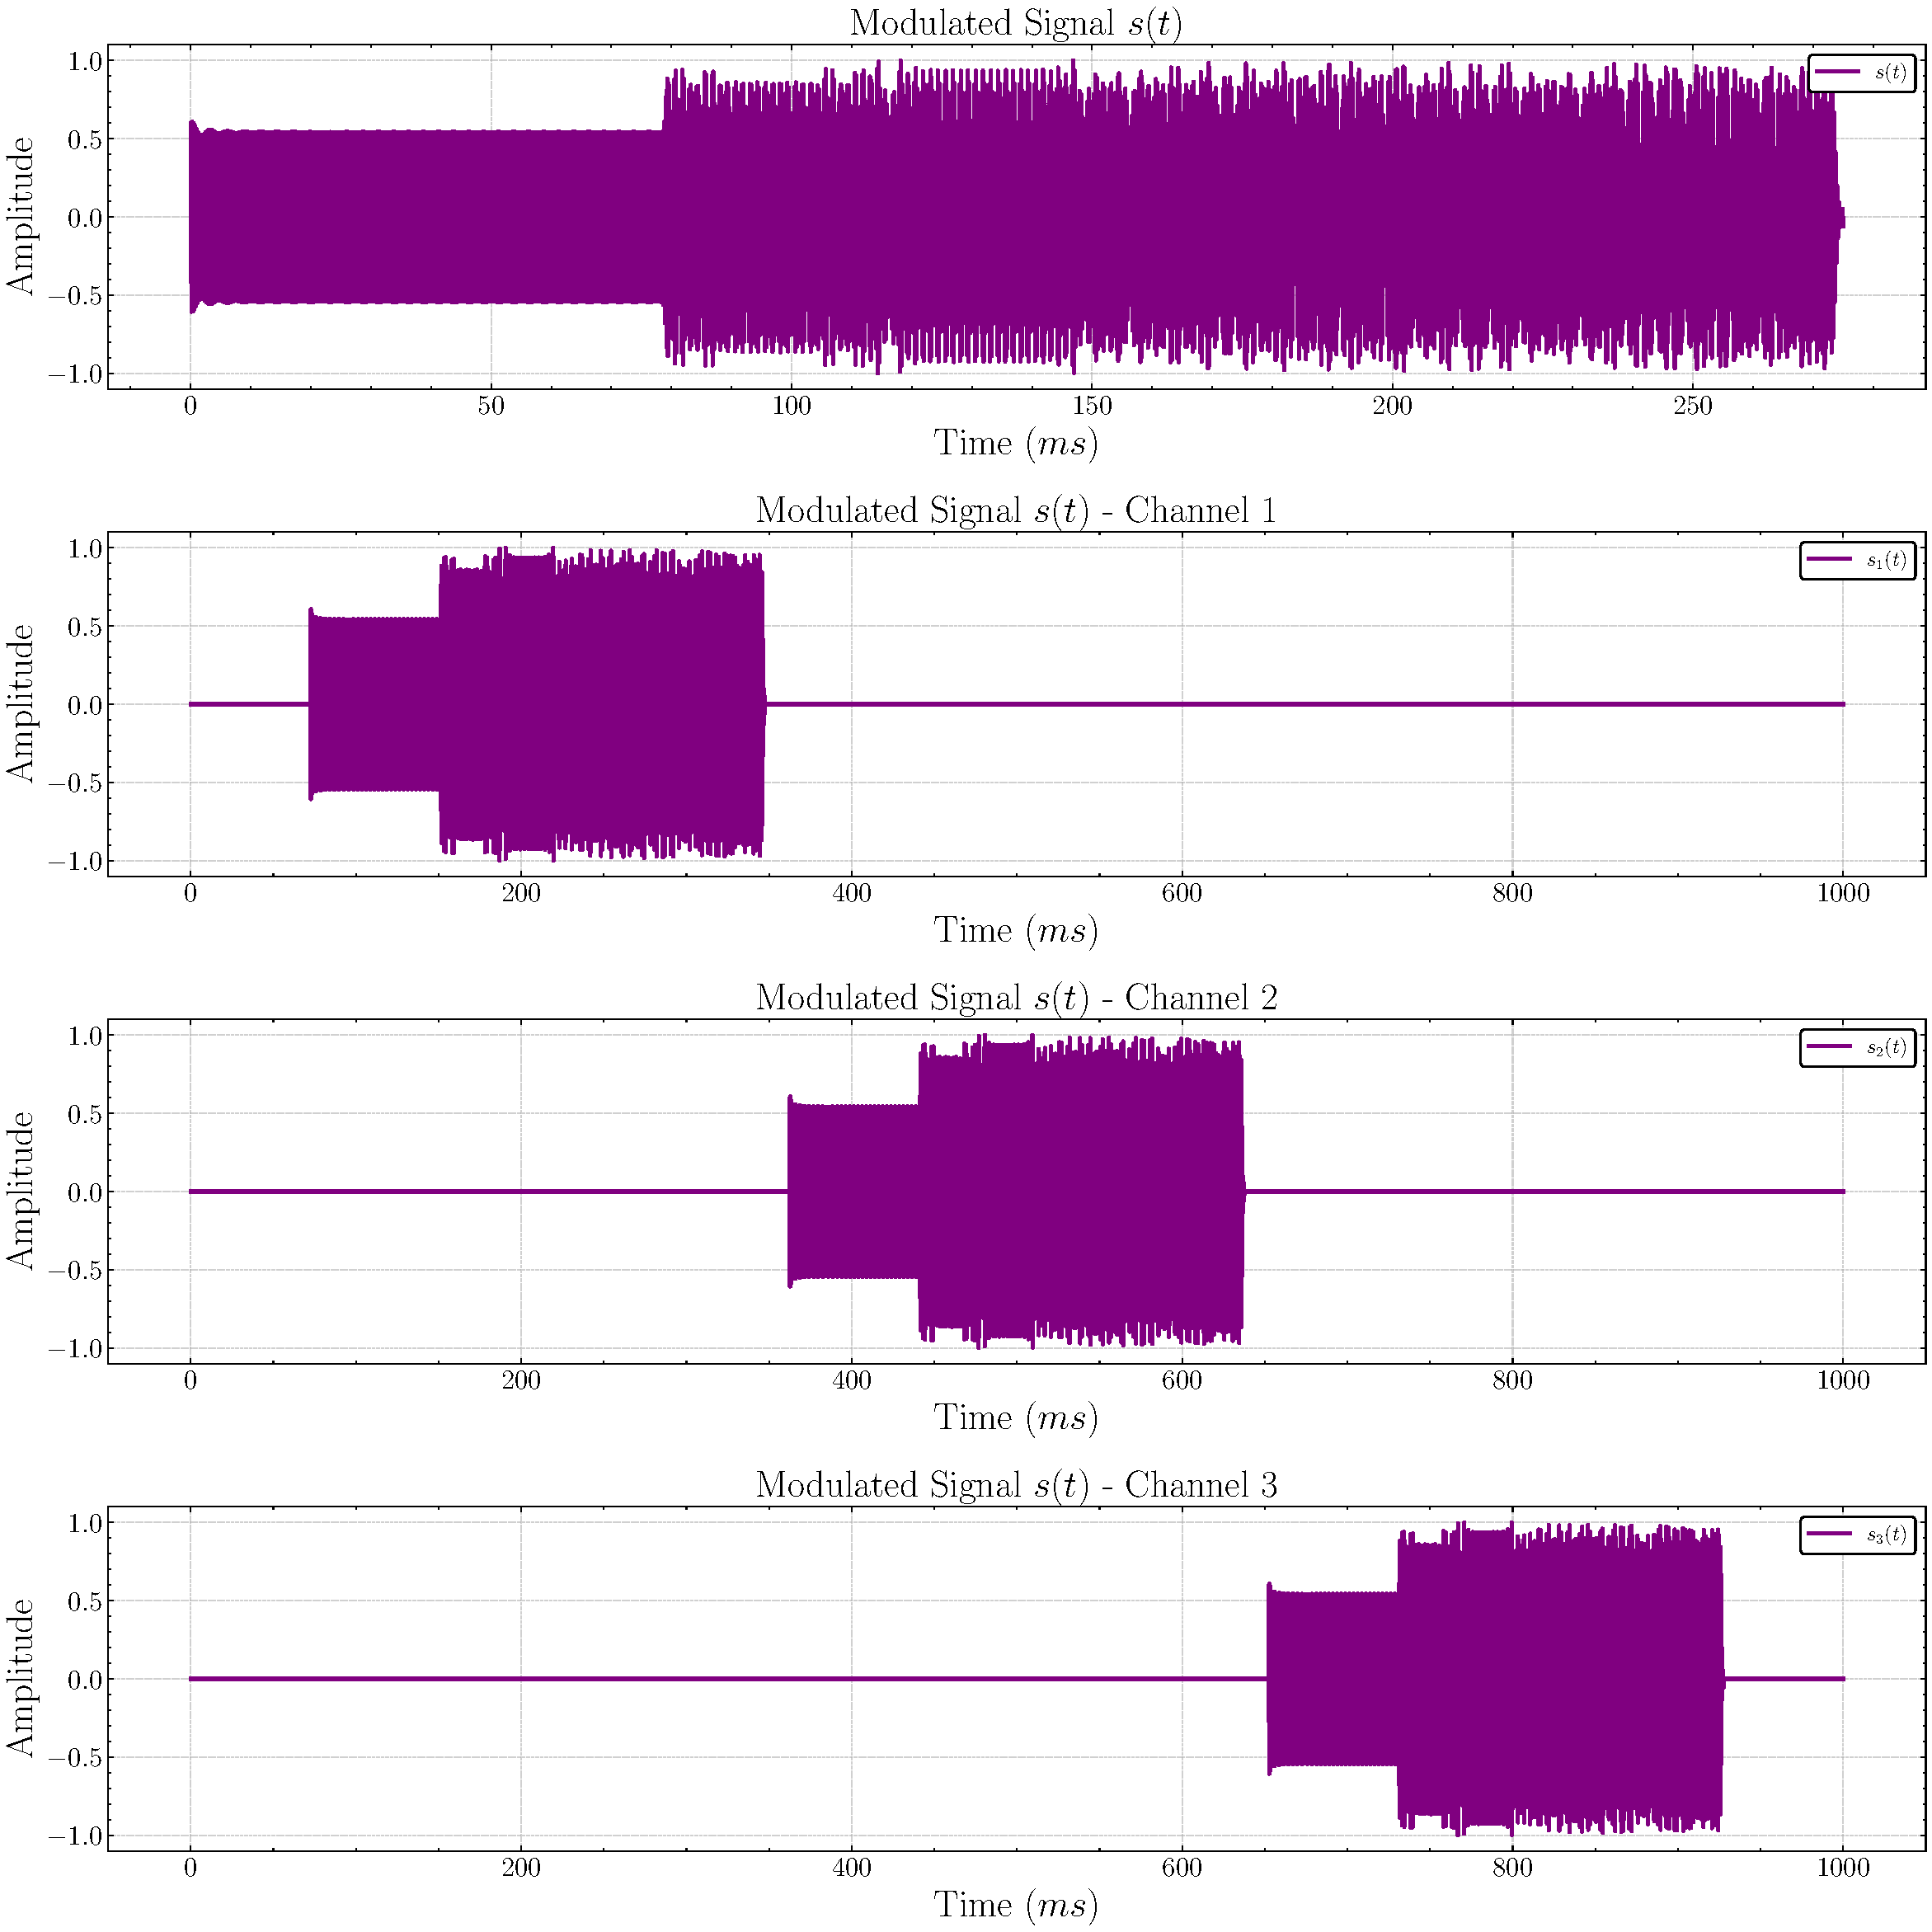
\includegraphics[width=\linewidth]{assets/cap3/example_channel_time_subchannels.pdf}
\end{figure}

\subsection{Geração de ruído AWGN}\label{sec:geracao_ruido}

\begin{figure}[H]
	\centering
	\caption{Adição de ruído ao canal}\label{fig:add_noise_time}
	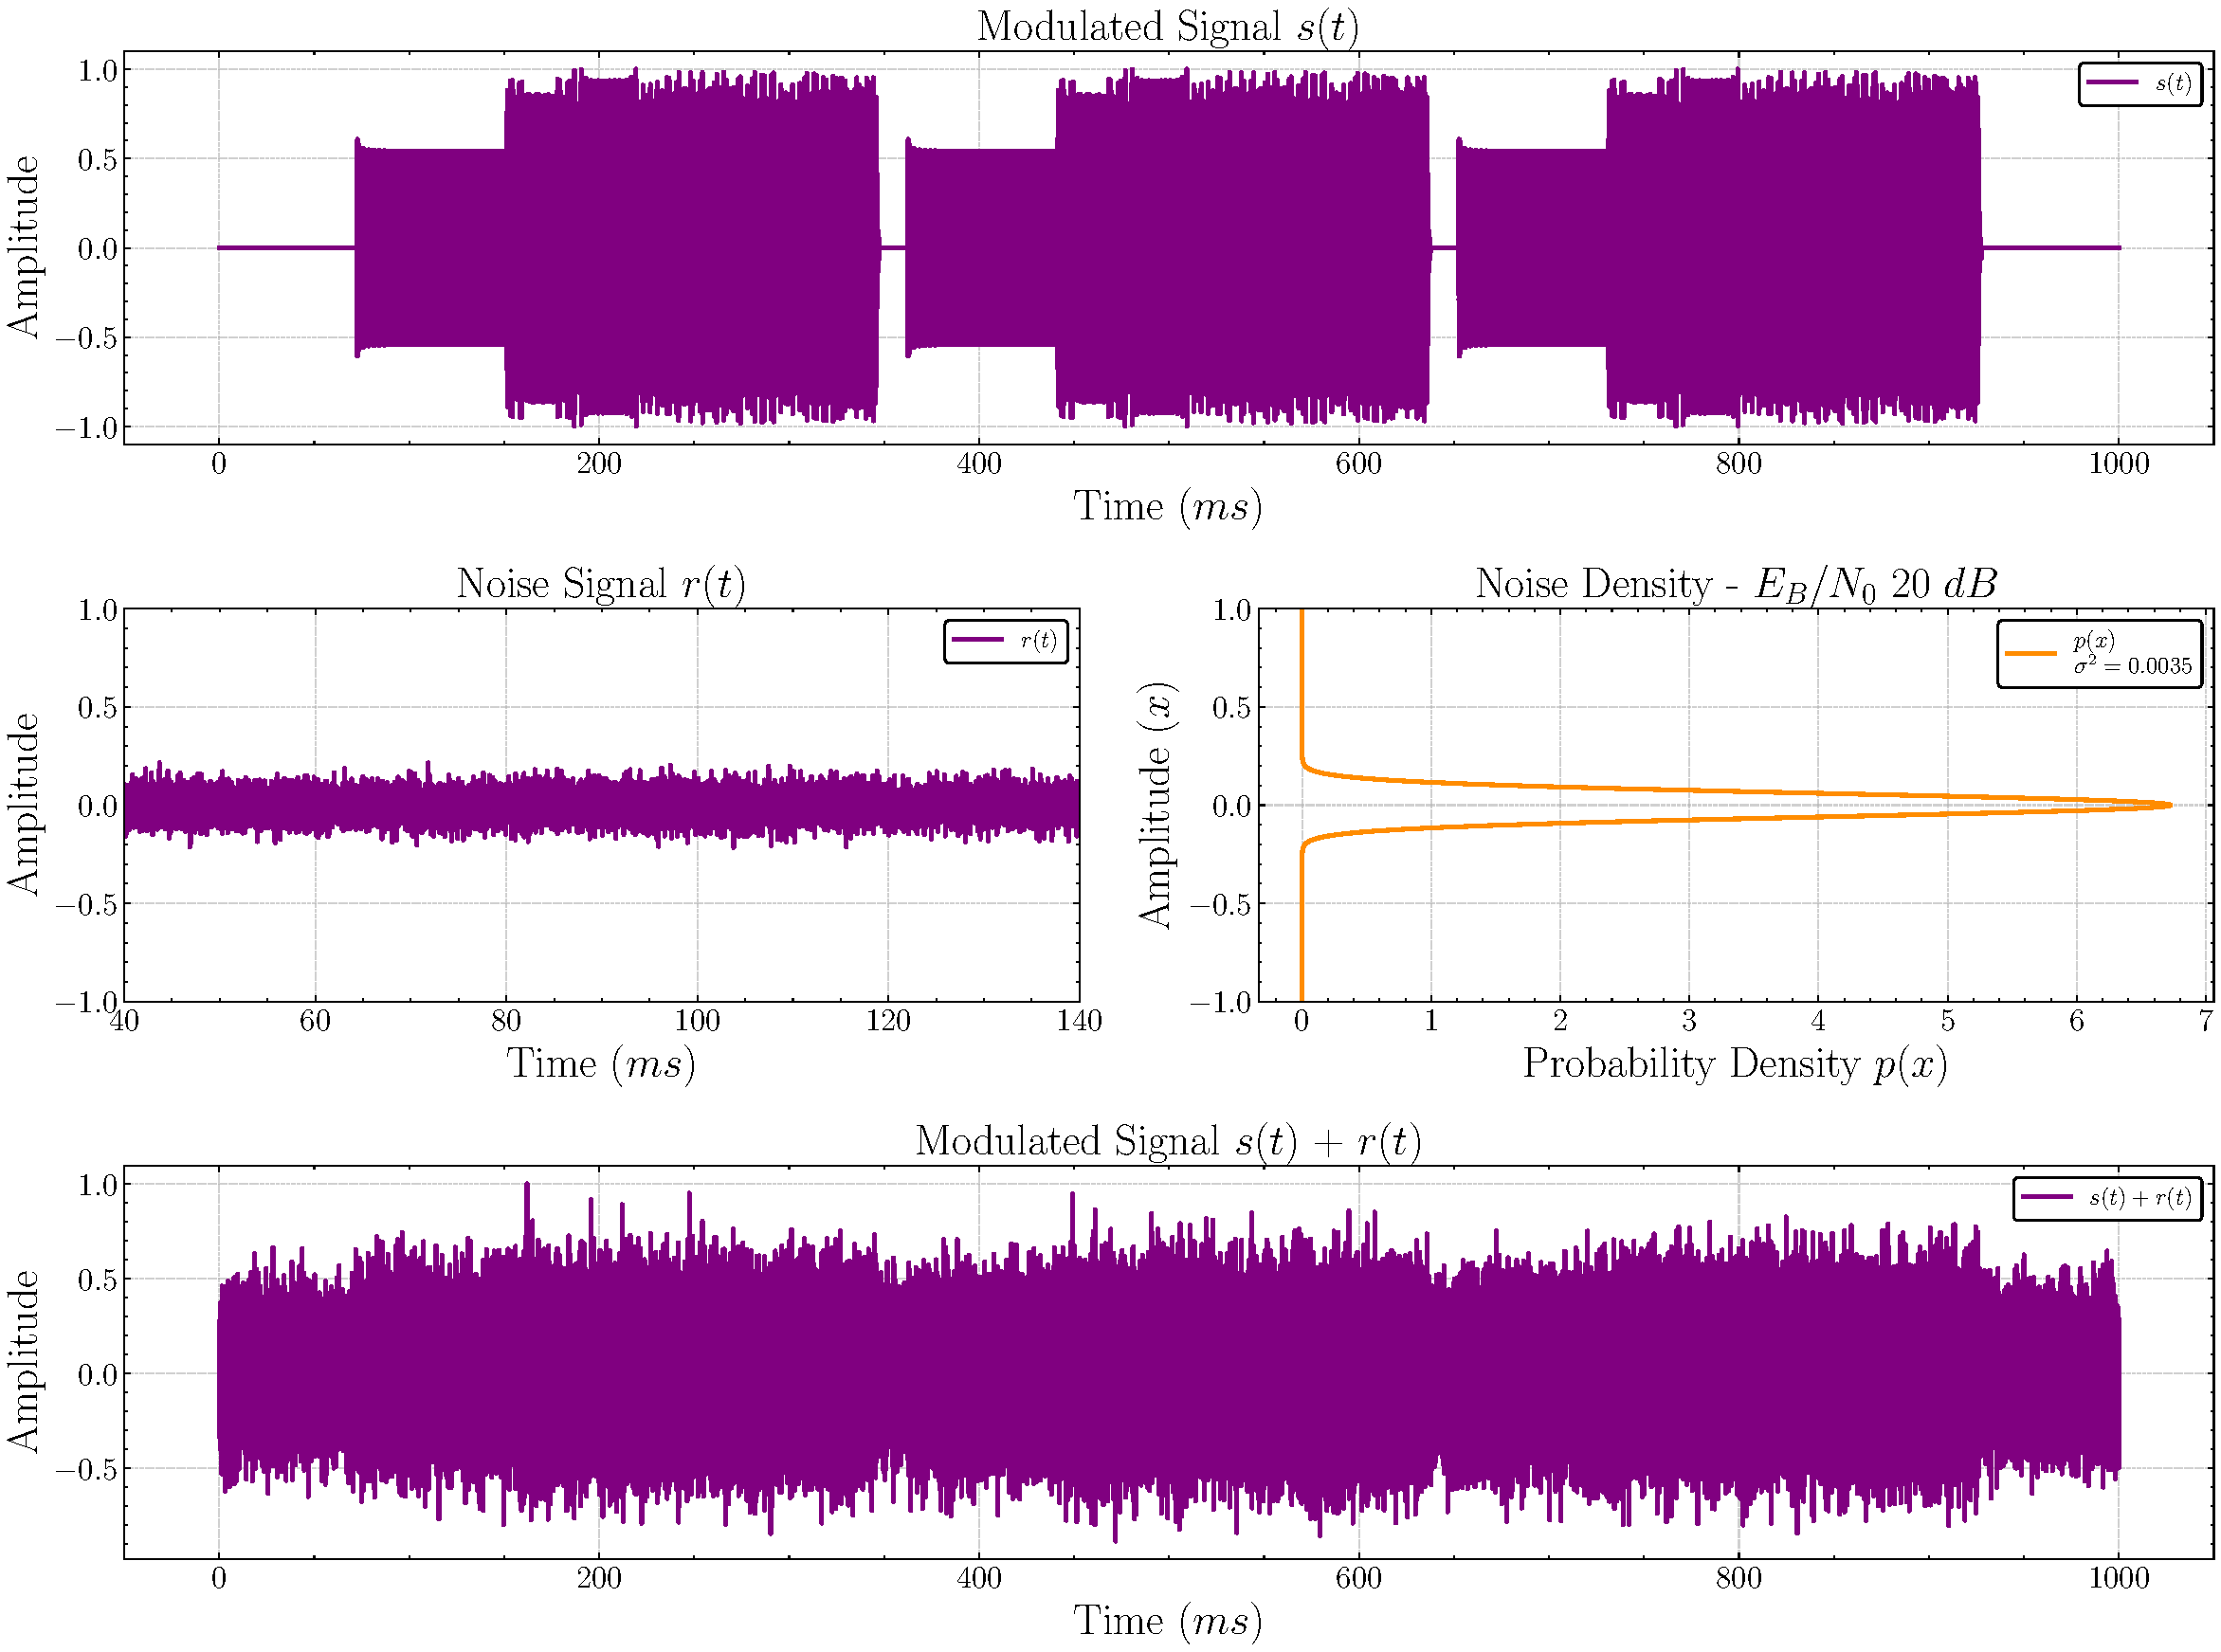
\includegraphics[width=\linewidth]{assets/cap3/example_channel_time_channel.pdf}
\end{figure}

\section{DETECÇÃO DE PORTADORA}\label{sec:detector}

\begin{figure}[H]
	\centering
	\caption{Diagrama de blocos da detecção de portadora}\label{fig:detector_diagram}
	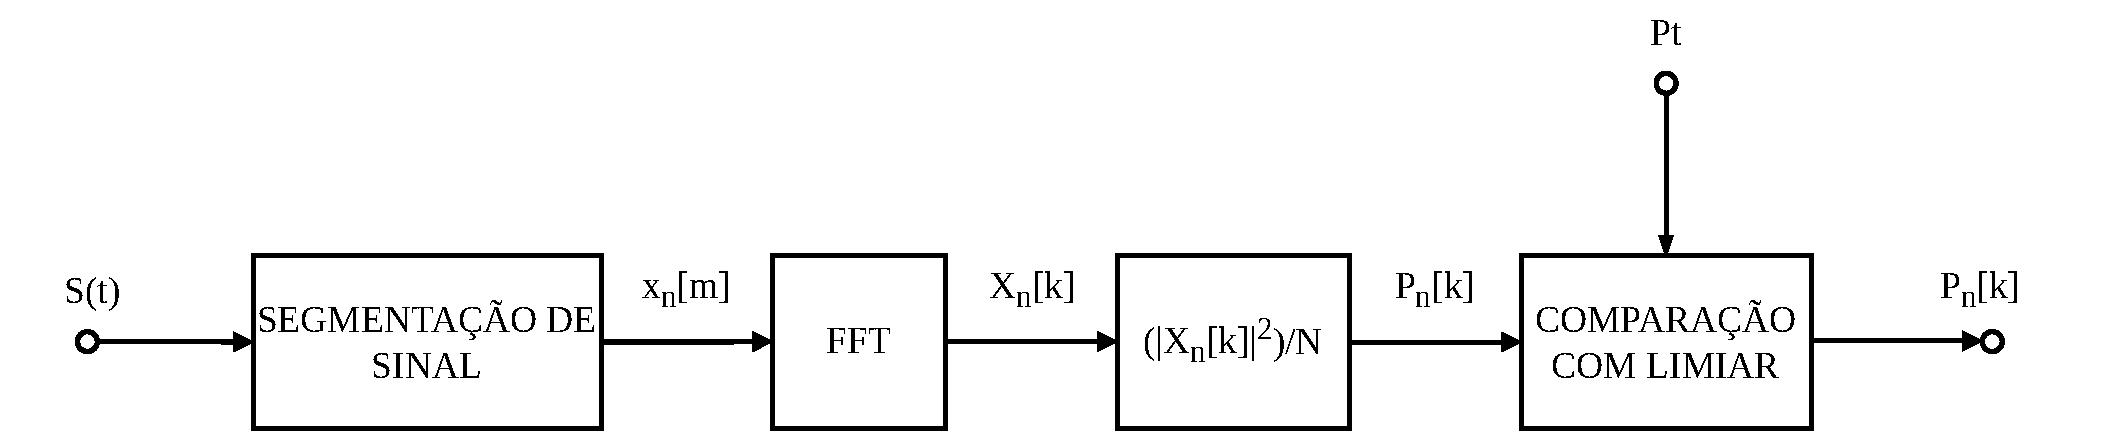
\includegraphics[width=\linewidth]{assets/diagrams/detector.pdf}
\end{figure}

\subsection{Segmentação do sinal recebido}\label{sec:segmentacao}

\begin{figure}[H]
	\centering
	\caption{Diagrama de waterfall do canal}\label{fig:waterfall}
	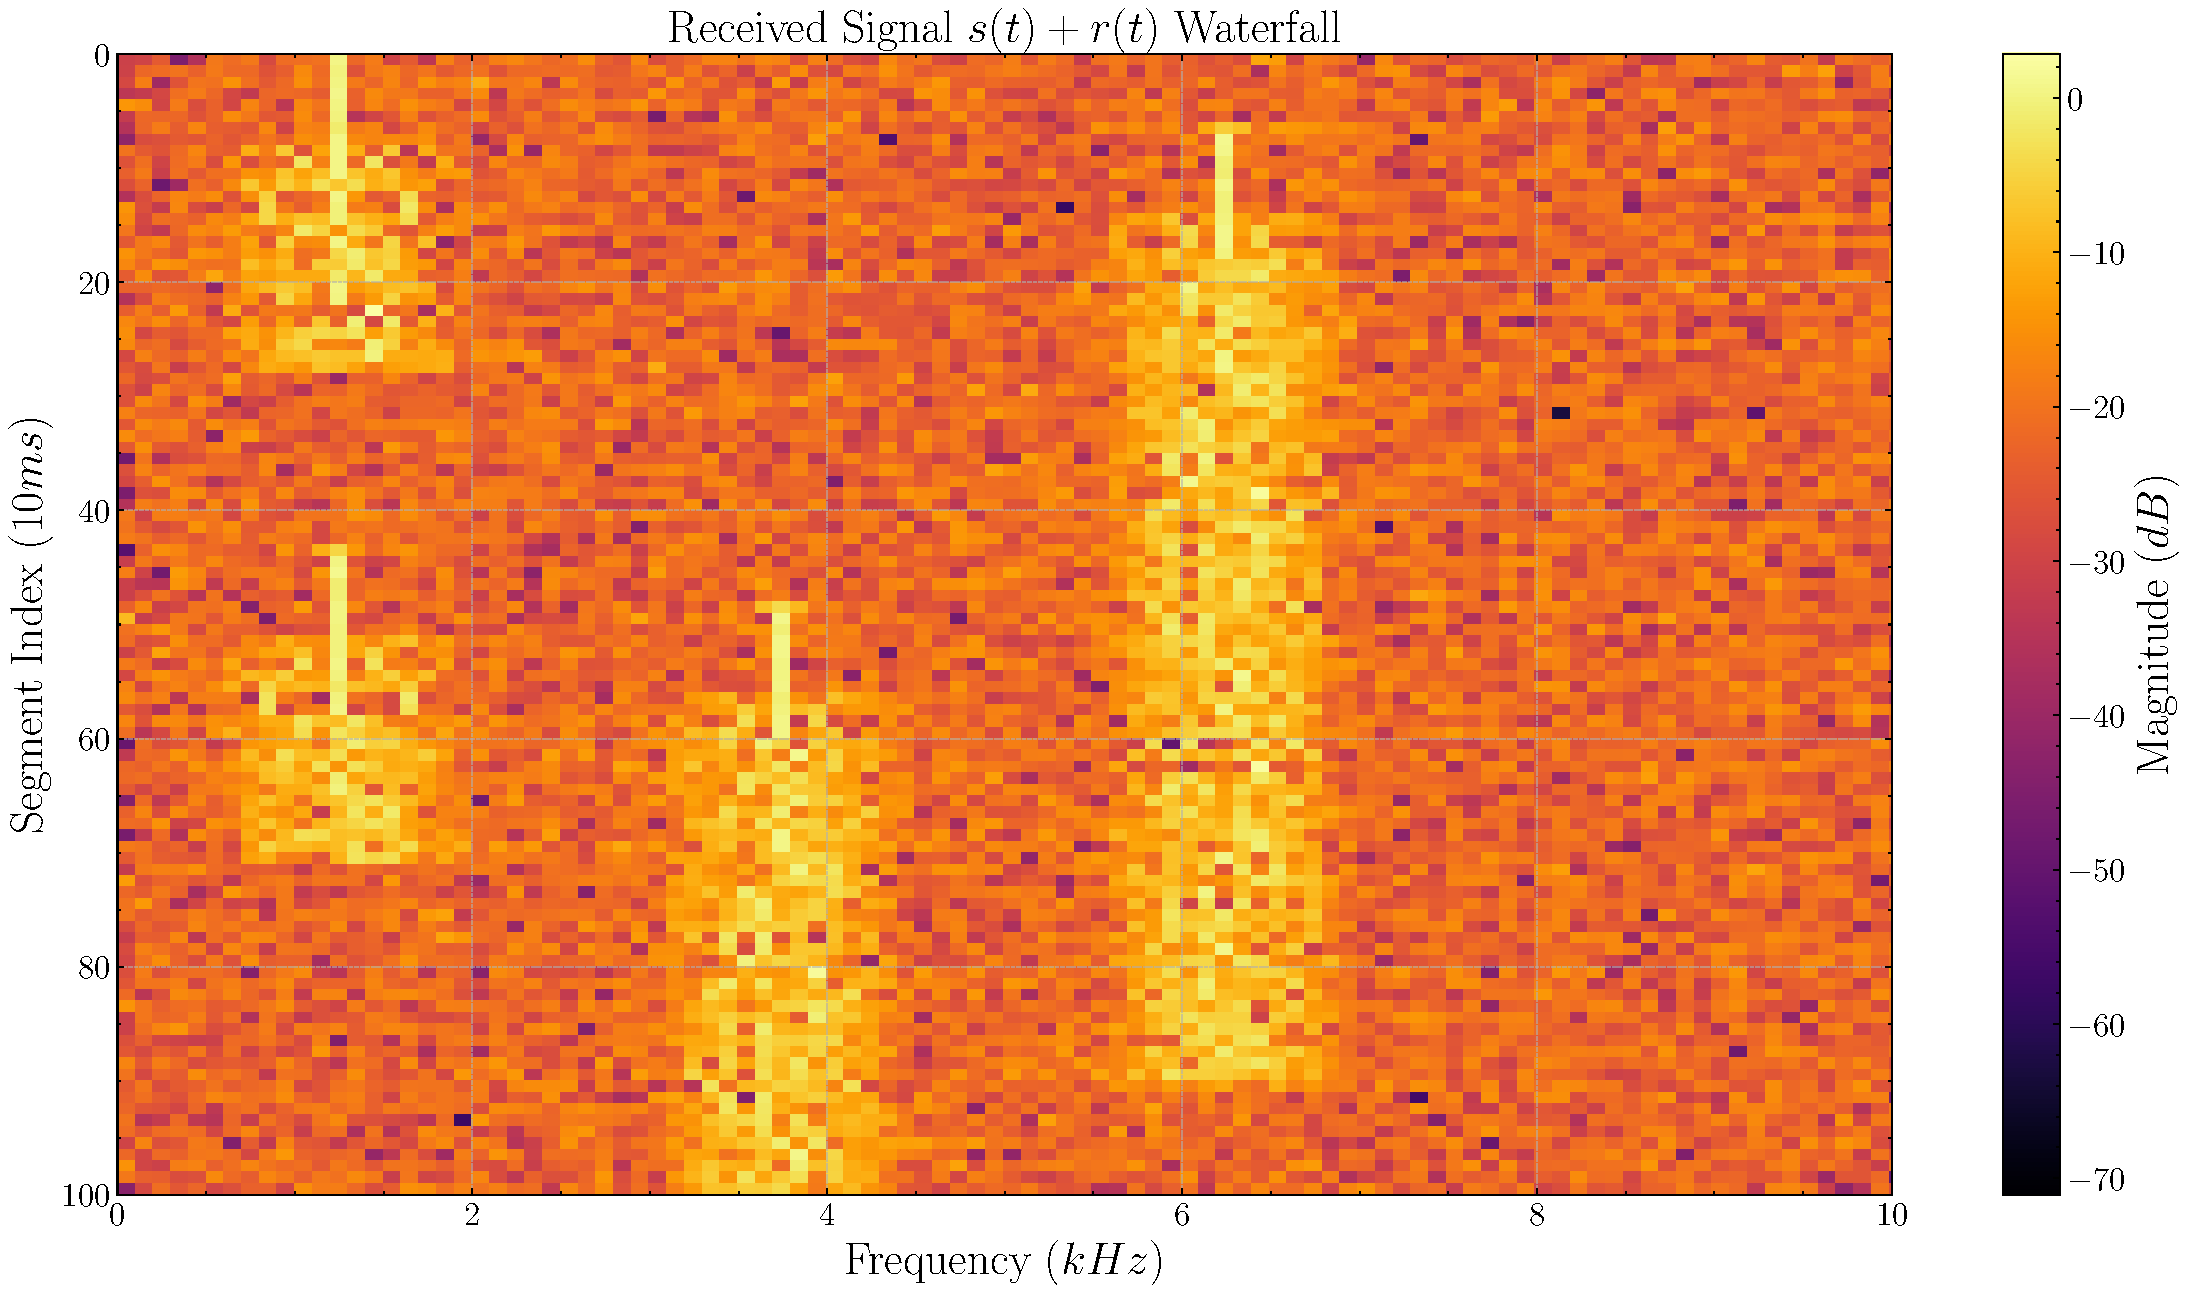
\includegraphics[width=\linewidth]{assets/cap3/example_detector_waterfall.pdf}
\end{figure}


\subsection{Detecção de componentes no espectro}\label{sec:comparacao_potencia}

\begin{figure}[H]
	\centering
	\caption{Detecção de componentes no espectro com base em $P_t$}\label{fig:freq_detection}
	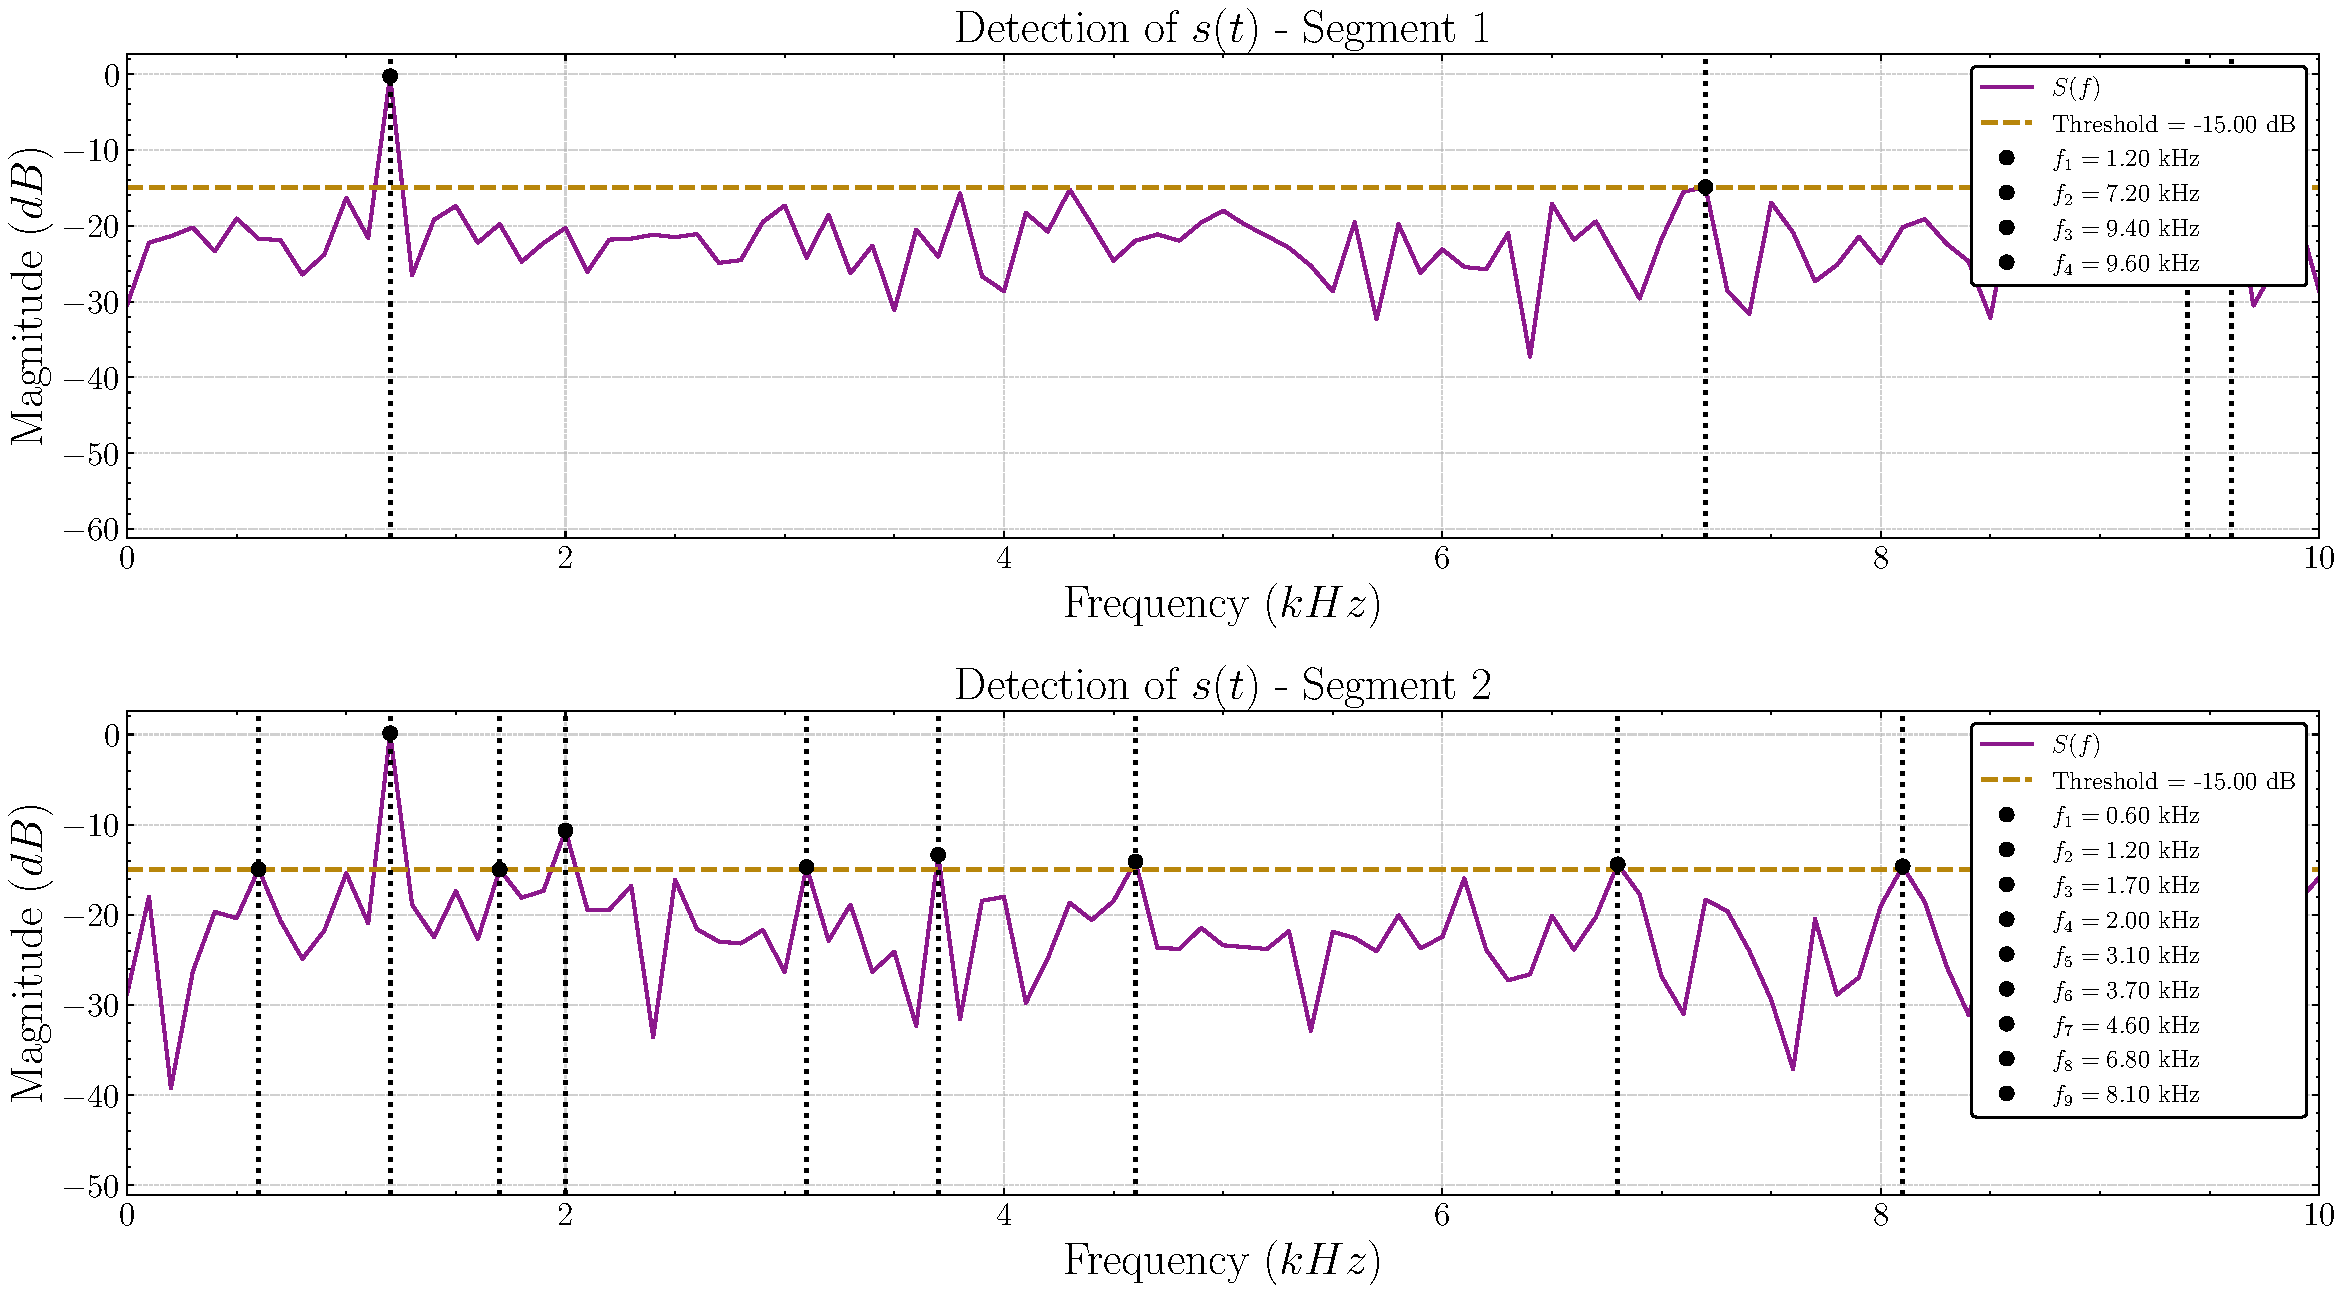
\includegraphics[width=\linewidth]{assets/cap3/example_detector_freq.pdf}
\end{figure}

\begin{figure}[H]
	\centering
	\caption{Diagrama de waterfall de detecção do canal}\label{fig:waterfall_detection}
	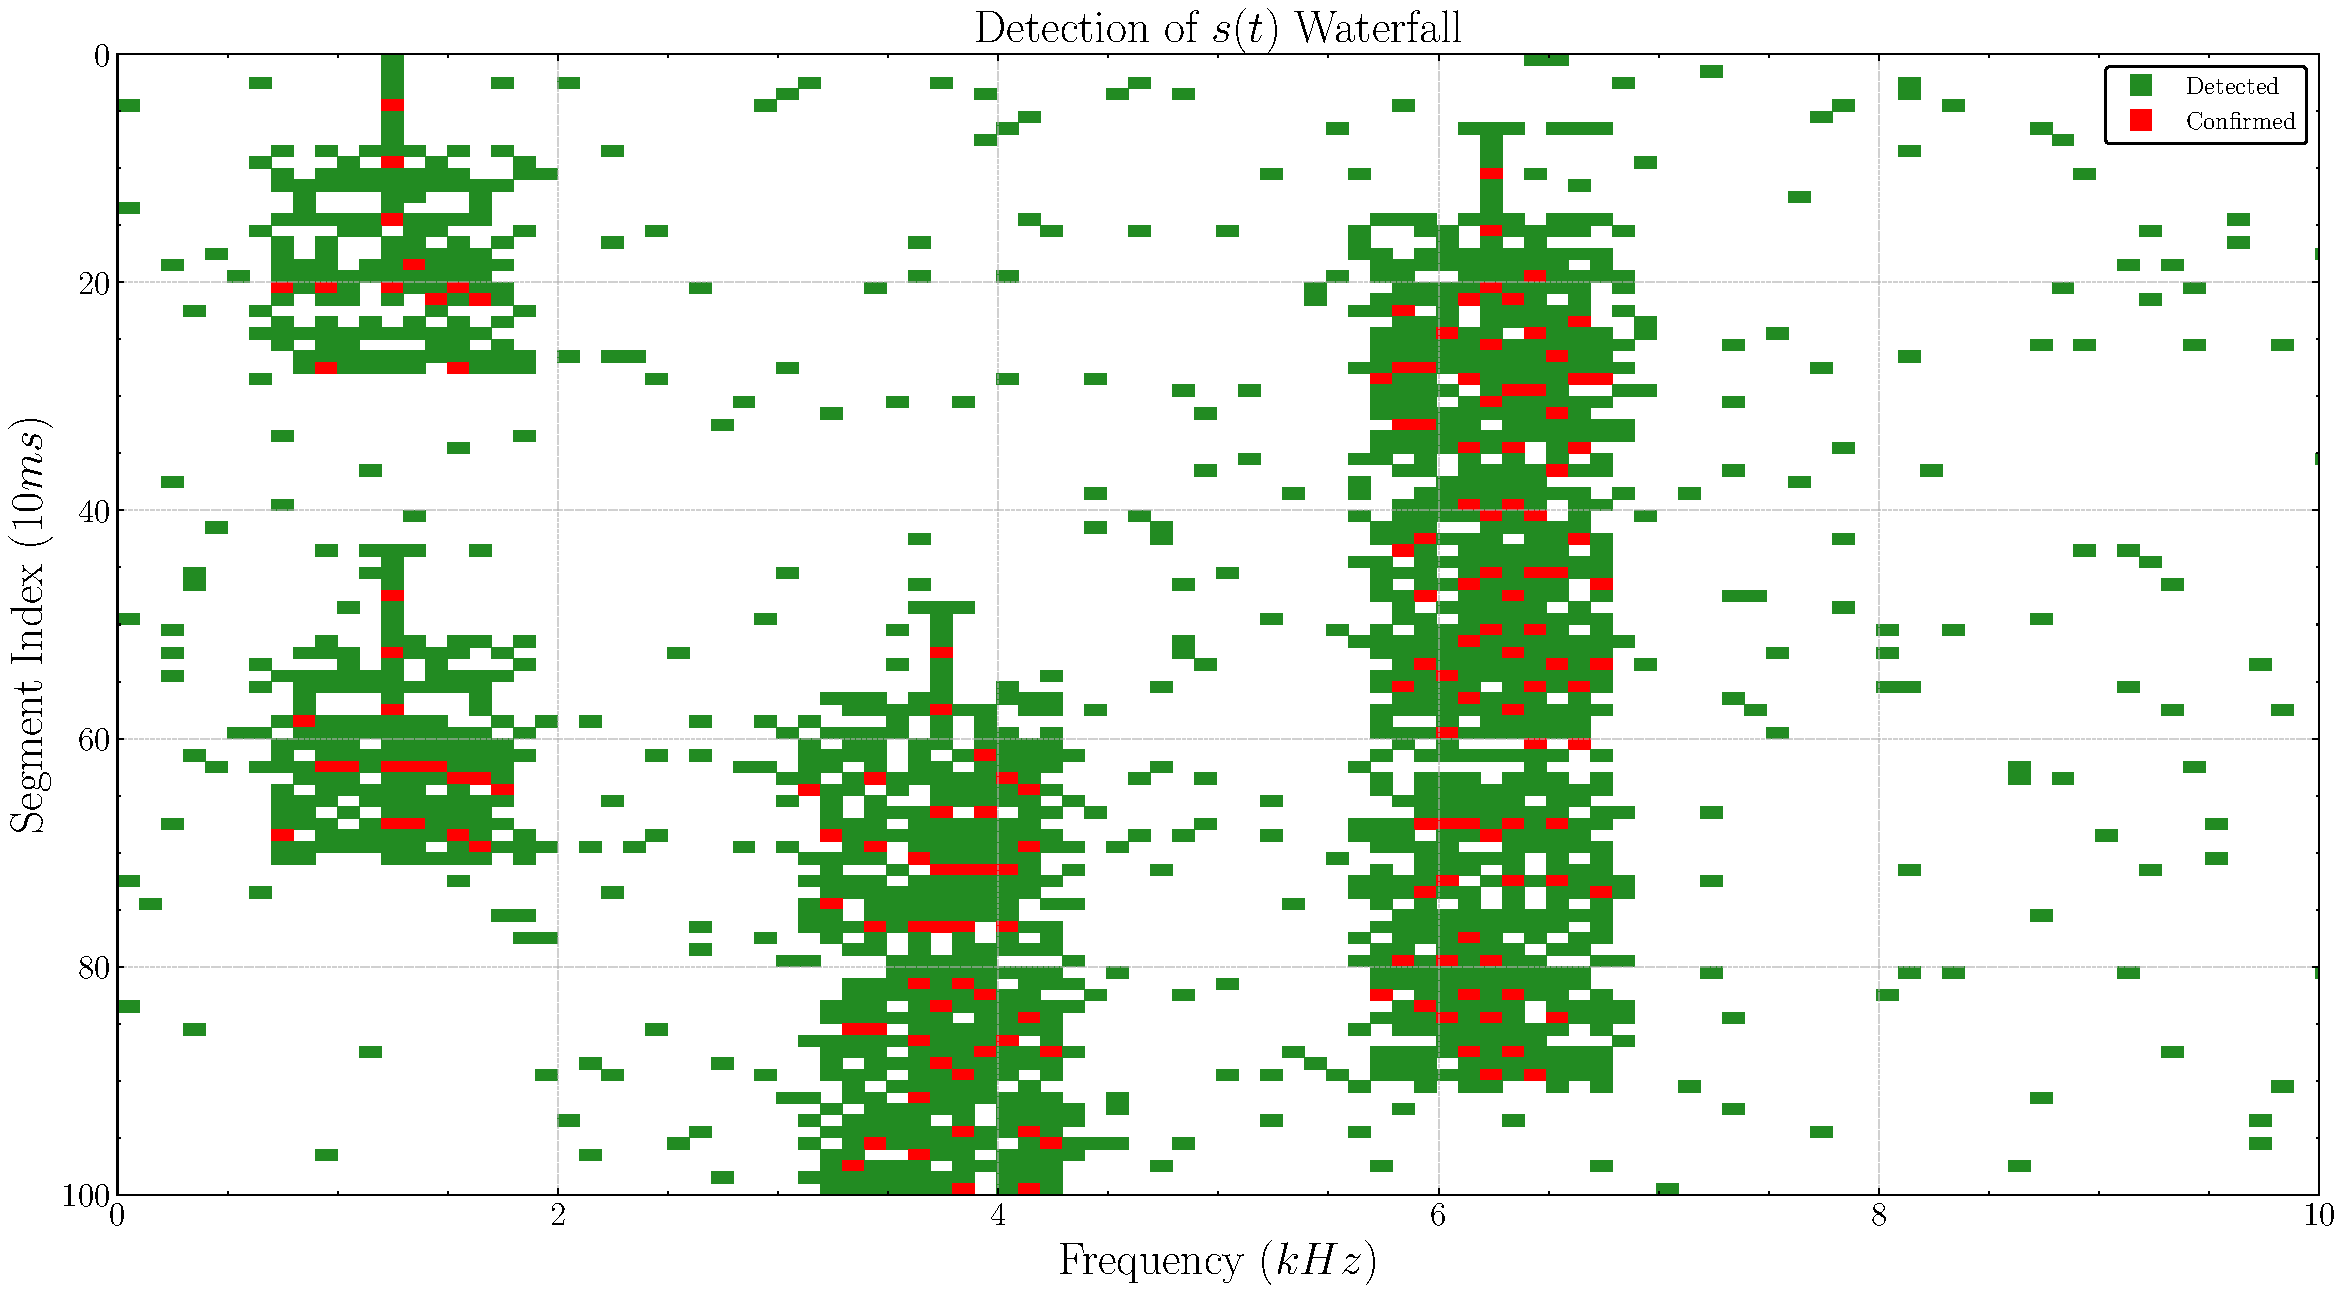
\includegraphics[width=\linewidth]{assets/cap3/example_detector_waterfall_detection.pdf}
\end{figure}


\subsection{Decisão de componentes detectadas}\label{sec:decisao}

\begin{figure}[H]
	\centering
	\caption{Diagrama de waterfall de decisão do canal}\label{fig:waterfall_decision}
	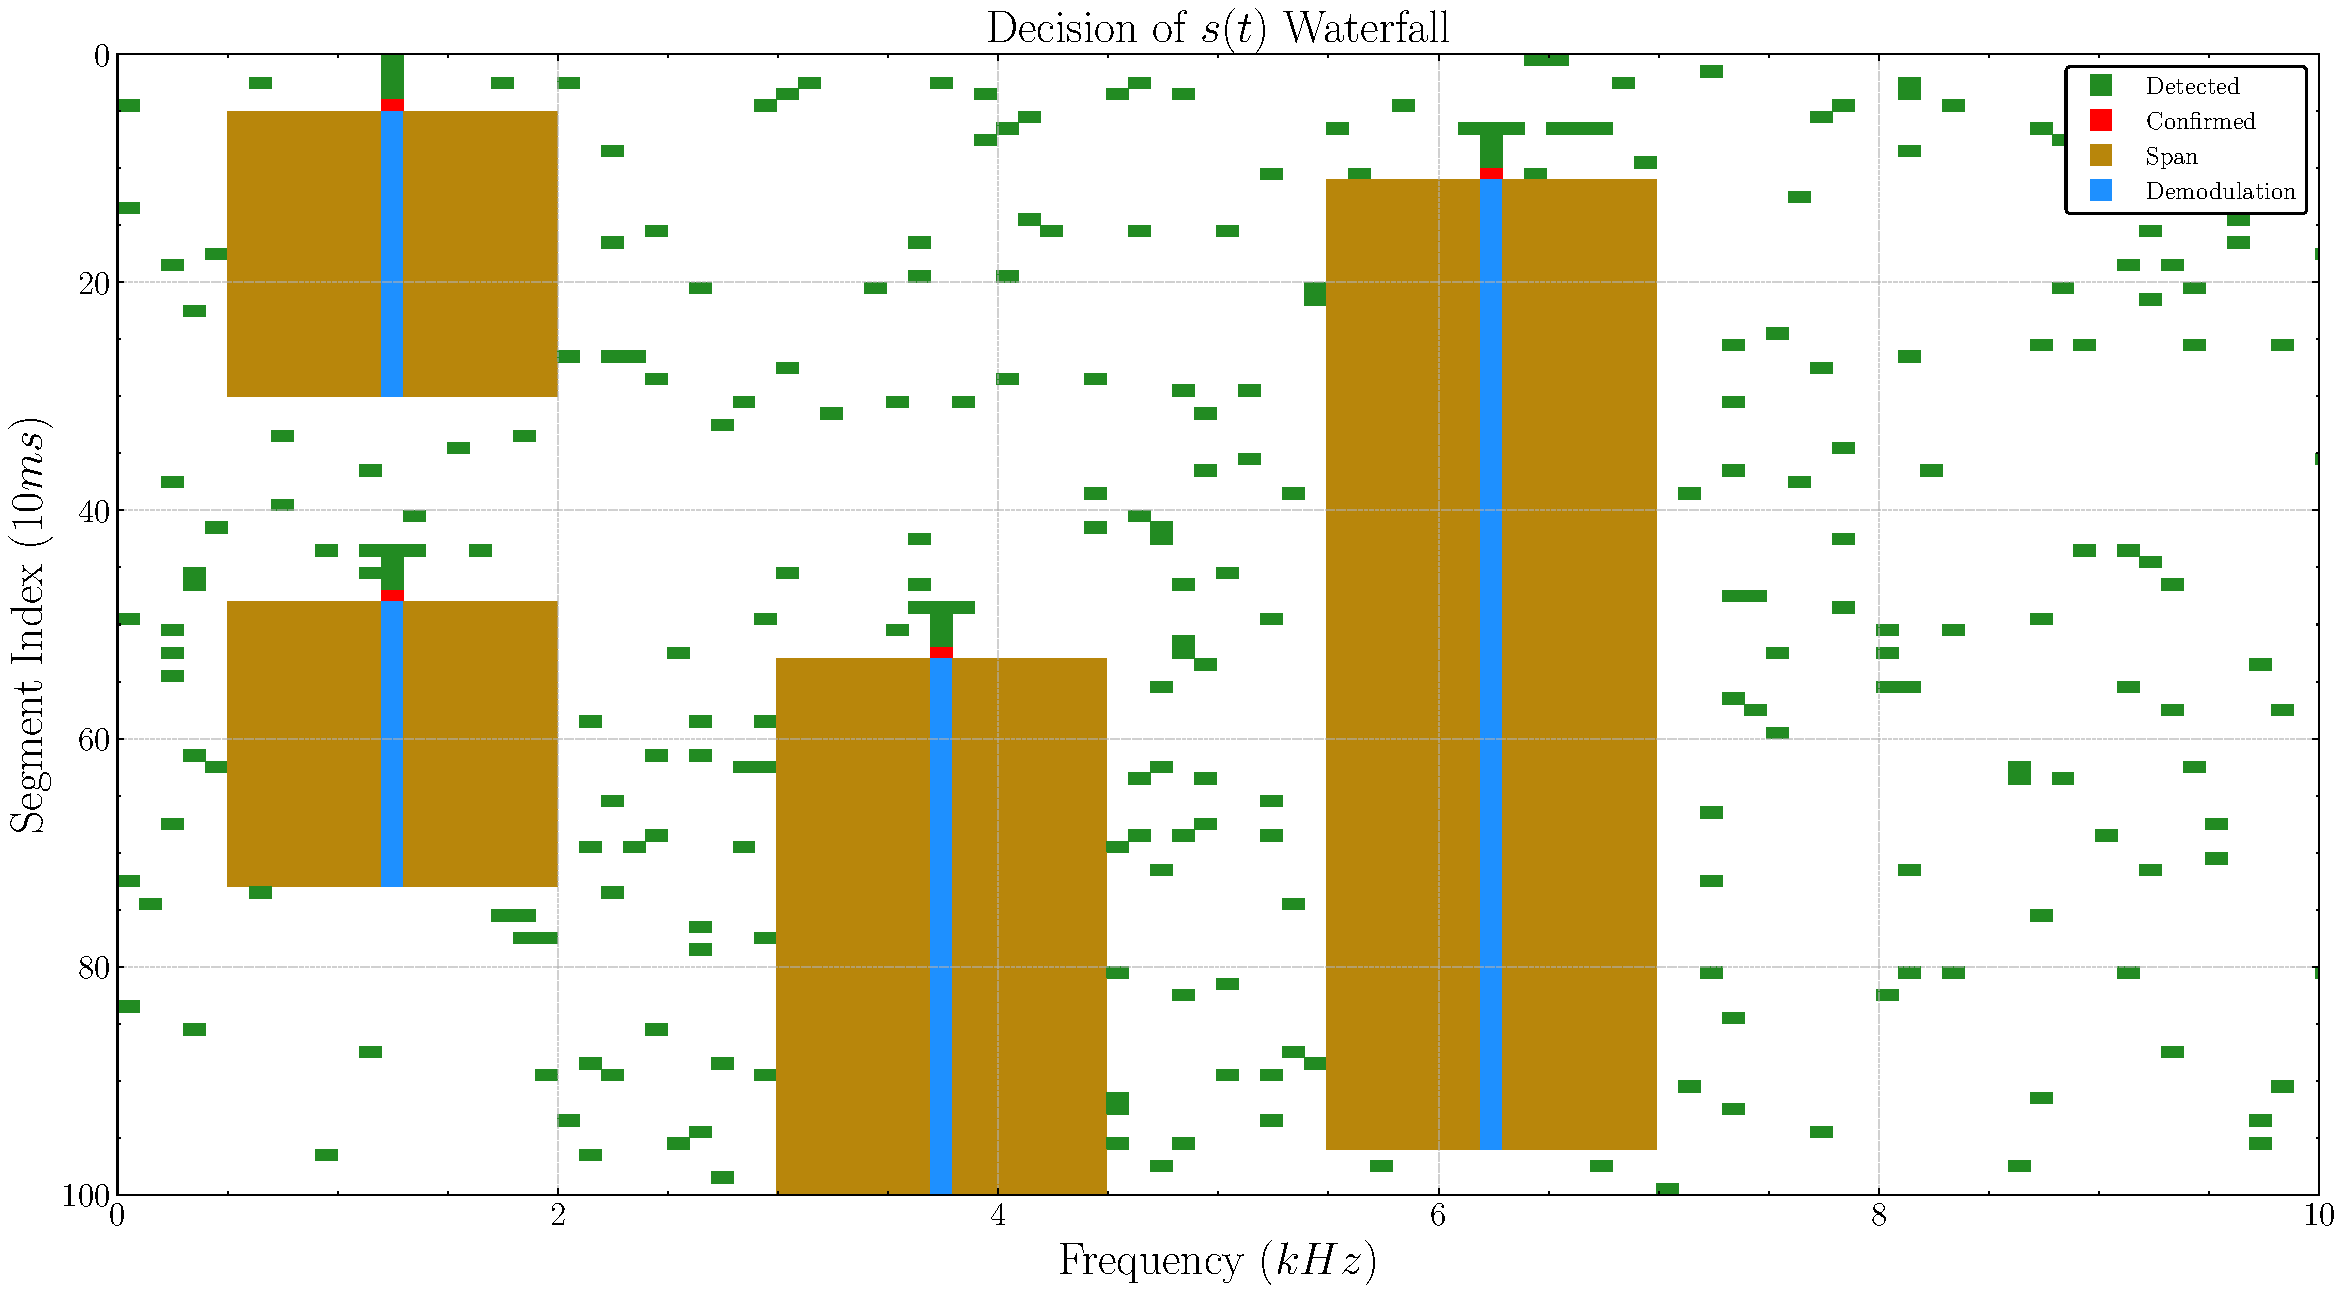
\includegraphics[width=\linewidth]{assets/cap3/example_detector_waterfall_decision.pdf}
\end{figure}

\subsection{Segmentação do sinal recebido para recepção}\label{sec:segmentacao_recepcao}

\section{CADEIA DE RECEPÇÃO}\label{sec:recepcao}    

\subsection{Demodulação banda base}\label{sec:demodulacao}

\begin{figure}[H]
	\centering
	\caption{Demodulação banda base dos canais $I$ e $Q$}\label{fig:receiver_demodulator}
	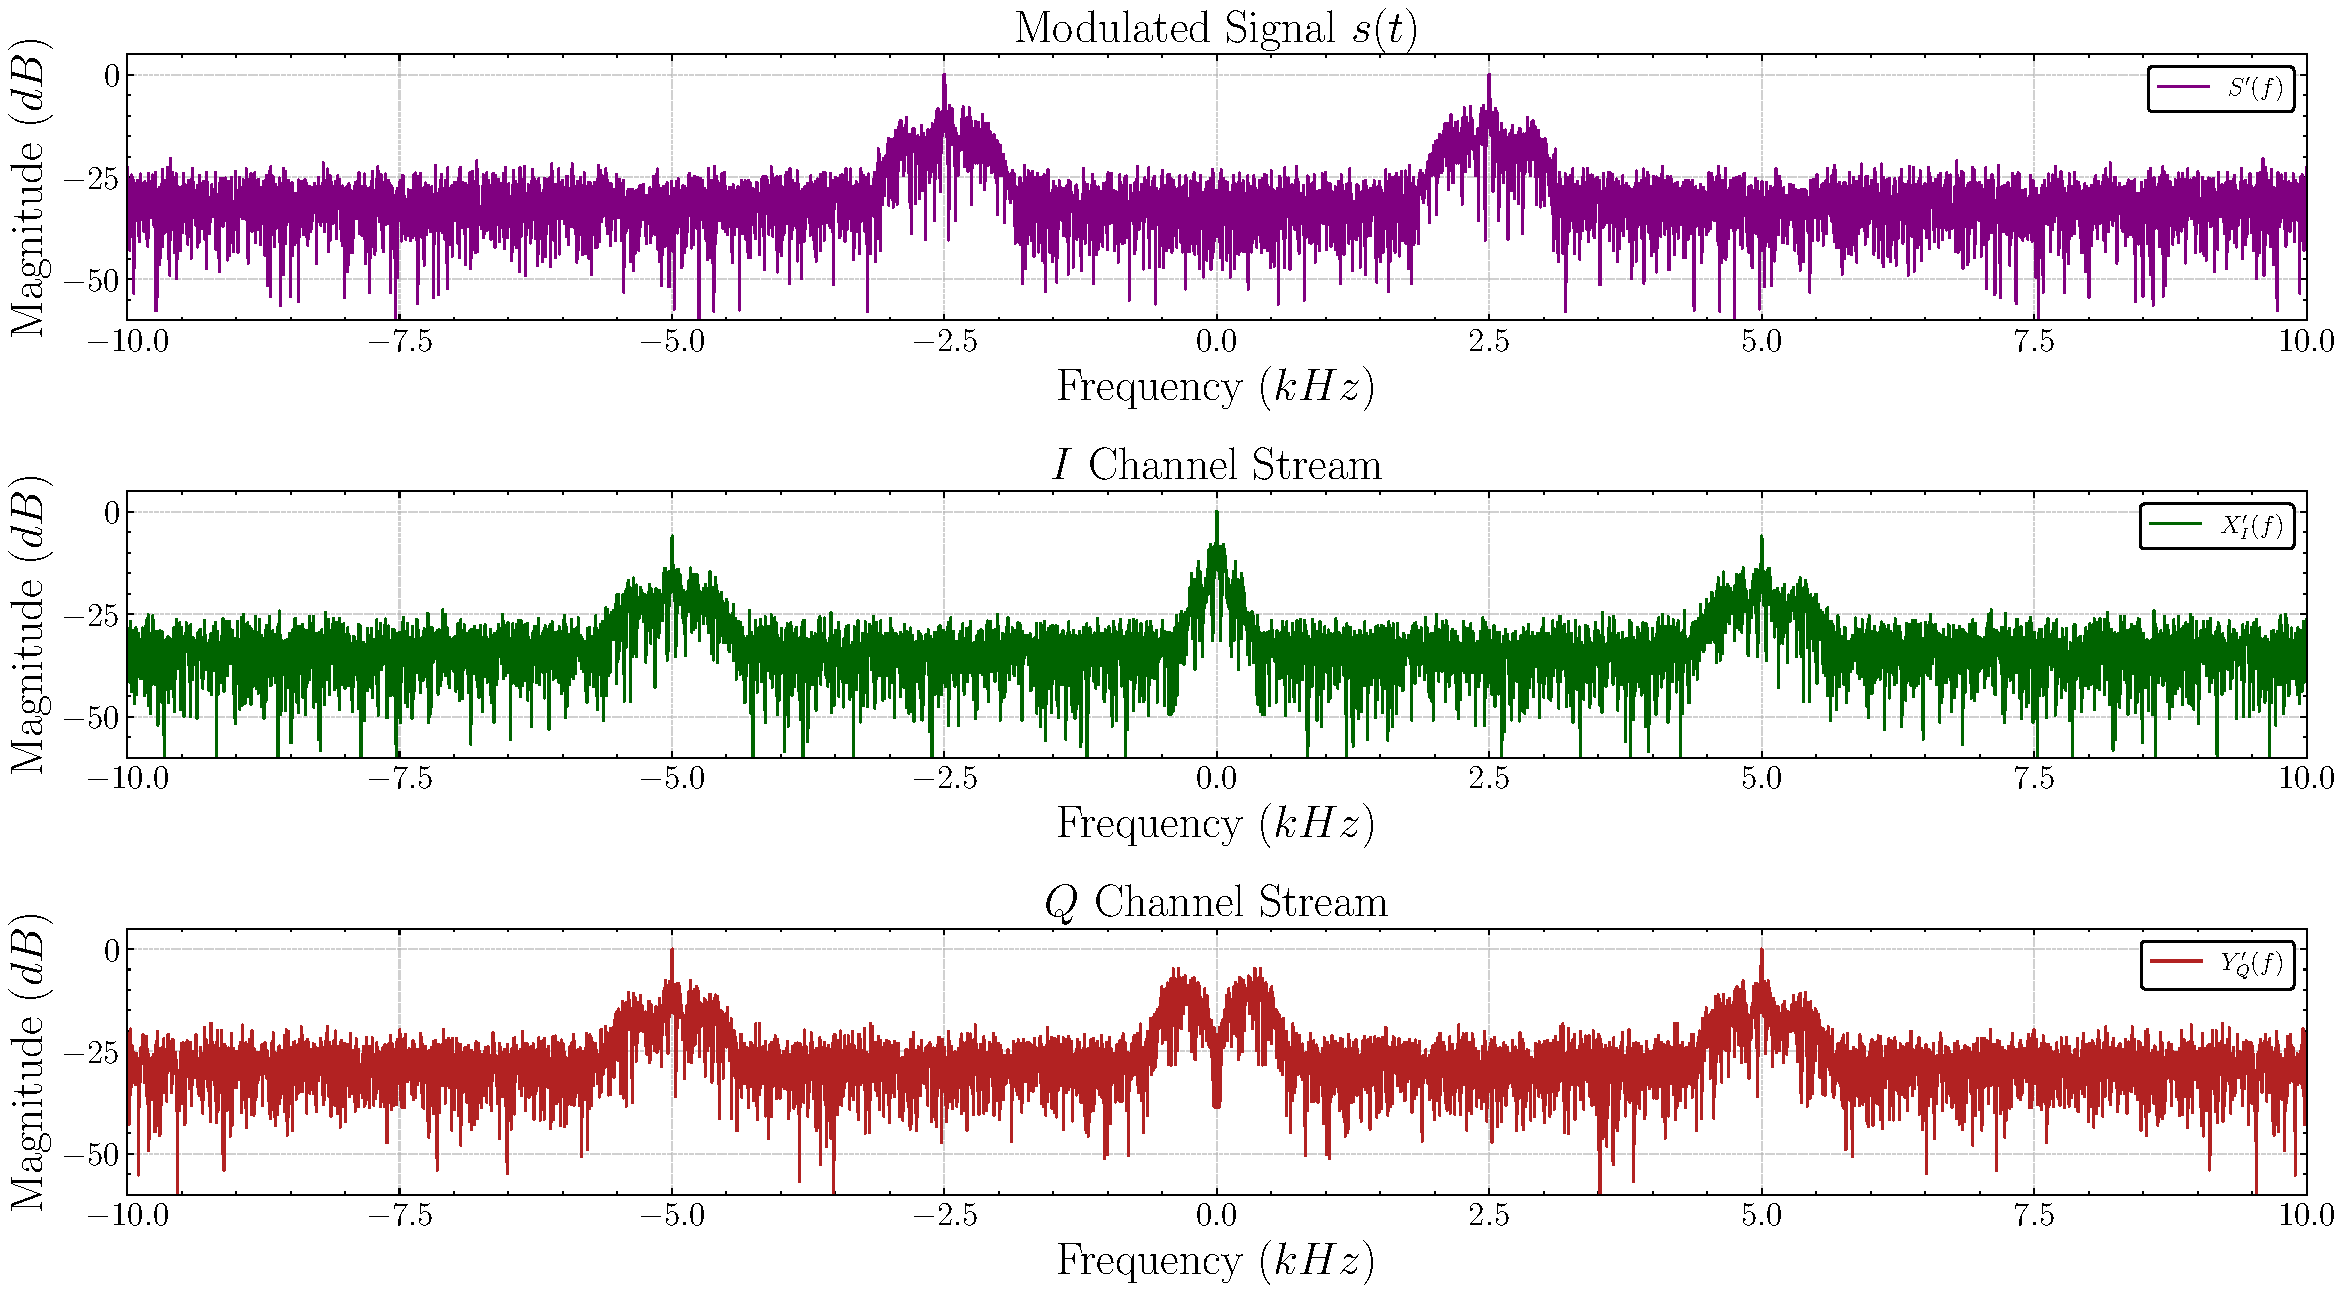
\includegraphics[width=\linewidth]{assets/cap3/receiver_demodulator_freq.pdf}
\end{figure}

\subsection{Filtragem}\label{sec:filtragem}

\begin{figure}[H]
	\centering
	\caption{Filtragem passa baixa dos canais $I$ e $Q$}\label{fig:receiver_lpf}
	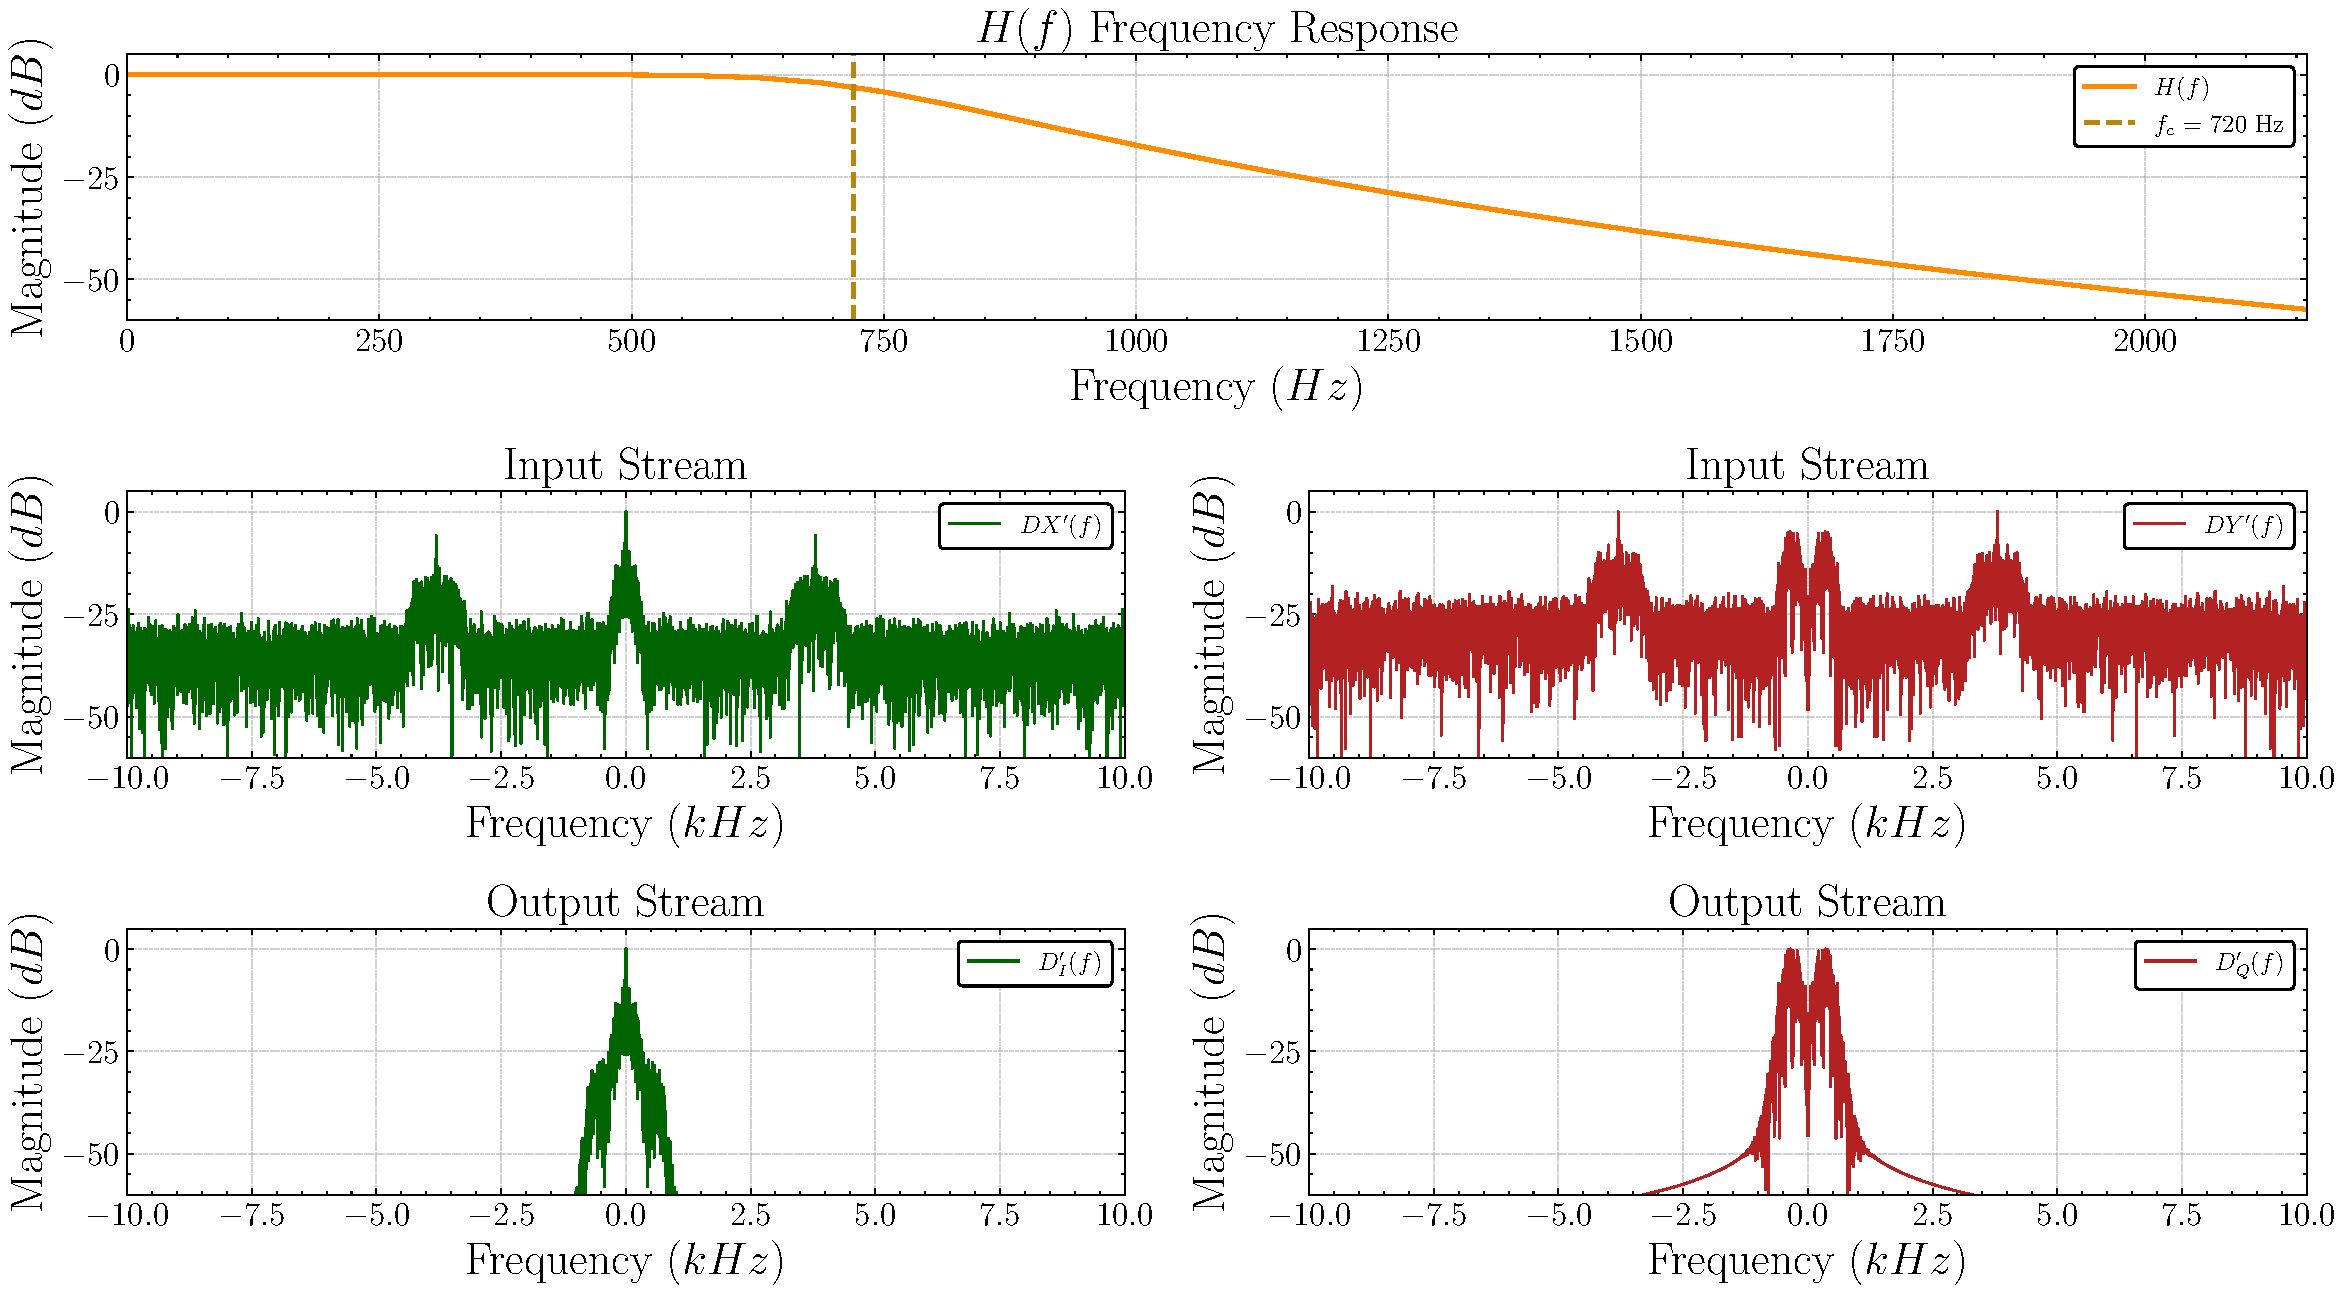
\includegraphics[width=\linewidth]{assets/cap3/receiver_lpf_freq.pdf}
\end{figure}

\begin{figure}[H]
	\centering
	\caption{Filtragem casada dos canais $I$ e $Q$}\label{fig:receiver_matchedfilter}
	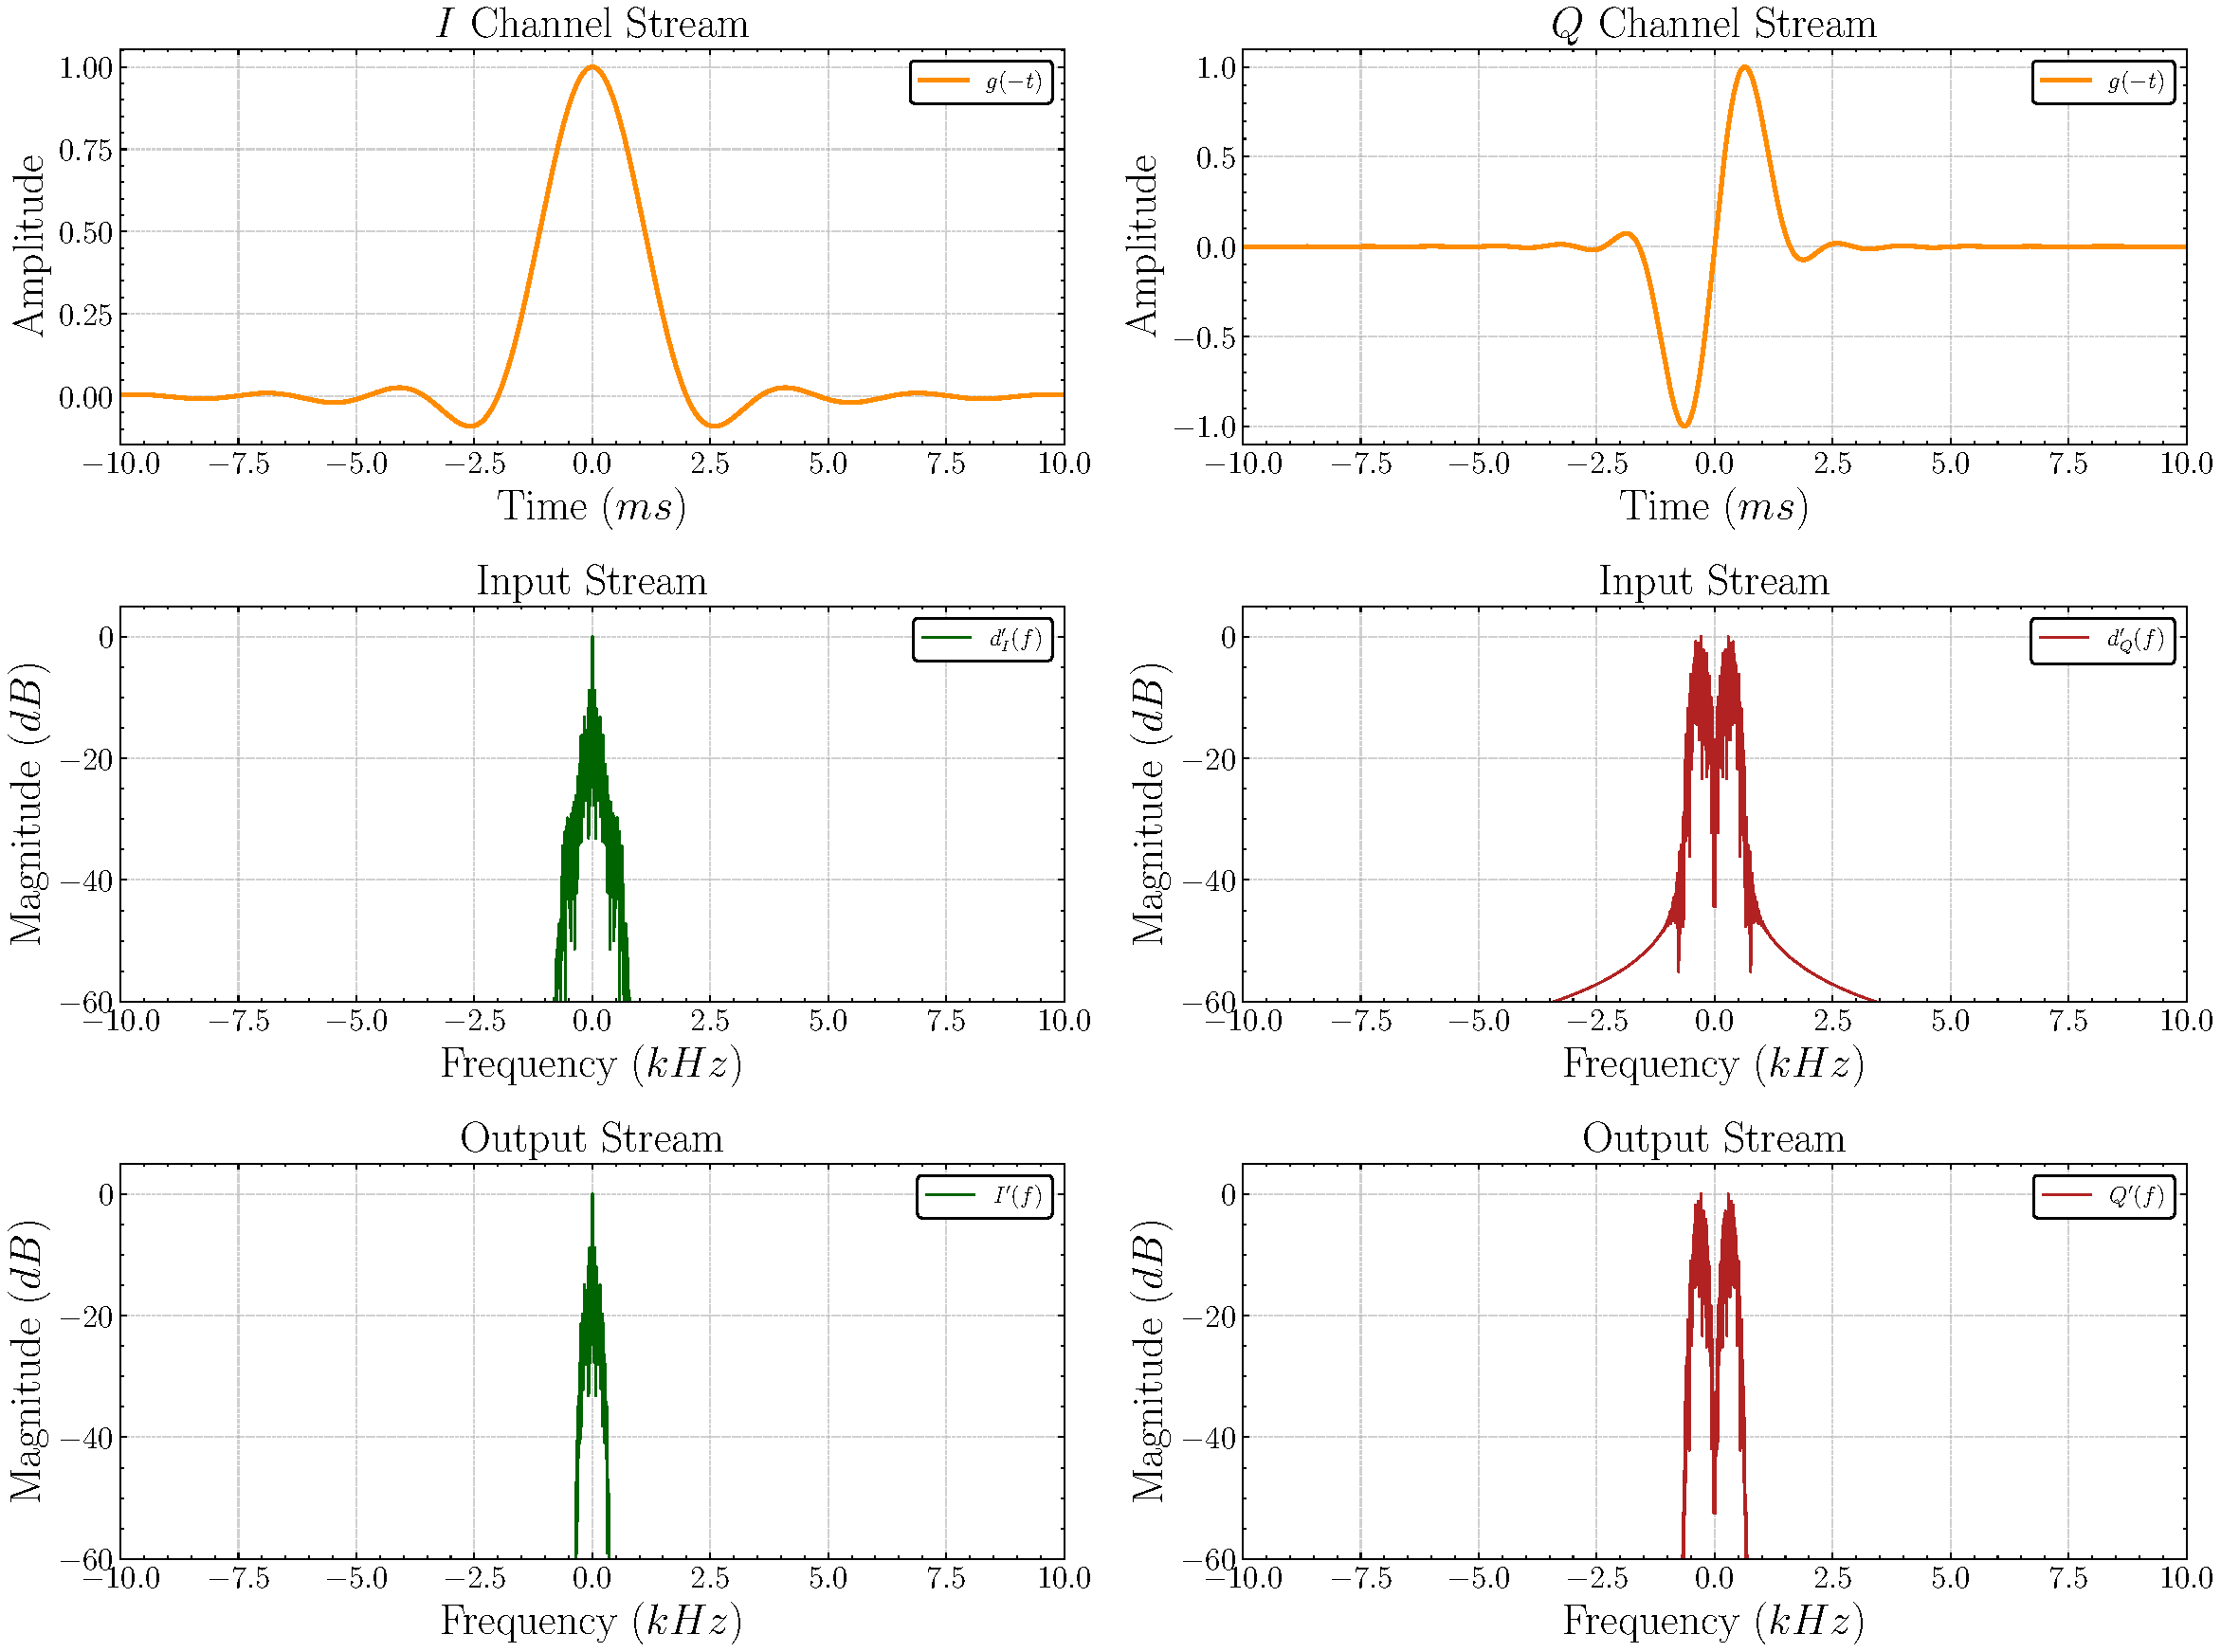
\includegraphics[width=\linewidth]{assets/cap3/receiver_mf_freq.pdf}
\end{figure}

\subsection{Sincronização de símbolos}\label{sec:sincronizacao}

\begin{figure}[H]
	\centering
	\caption{Diagrama de blocos para montagem do vetor de sincronismo}\label{fig:receiver_sync_diagram}
	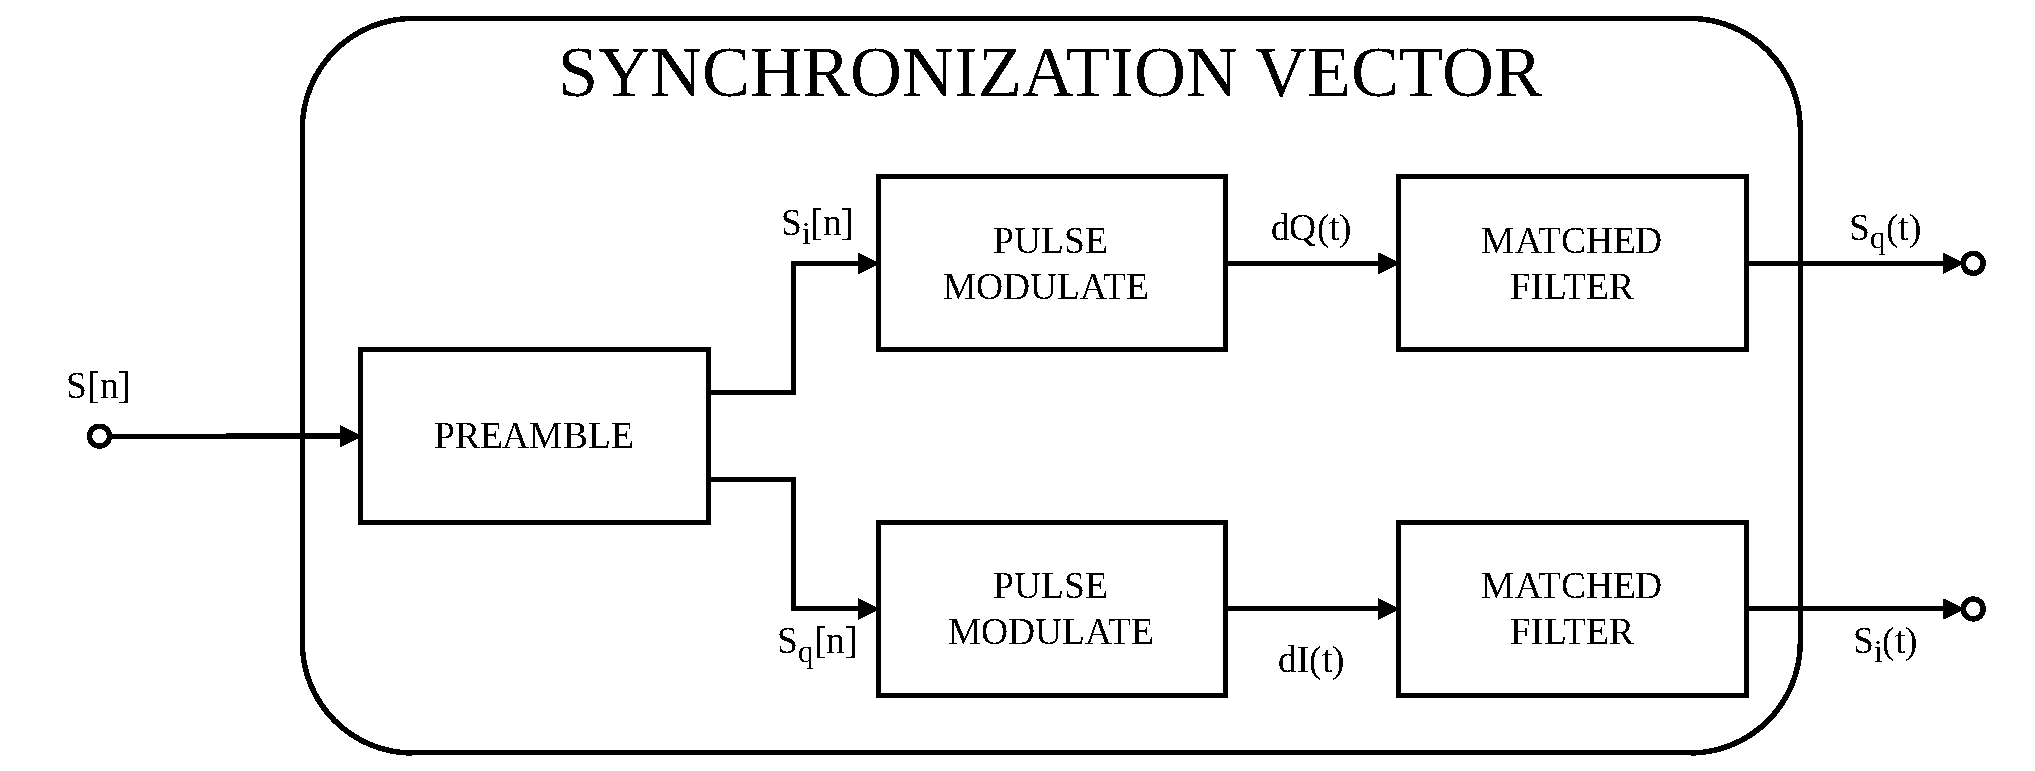
\includegraphics[width=\linewidth]{assets/diagrams/sync.pdf}
\end{figure}


\begin{figure}[H]
	\centering
	\caption{Vetor de amostras esperadas para sincronismo com $I$ e $Q$}\label{fig:receiver_sync_word}
	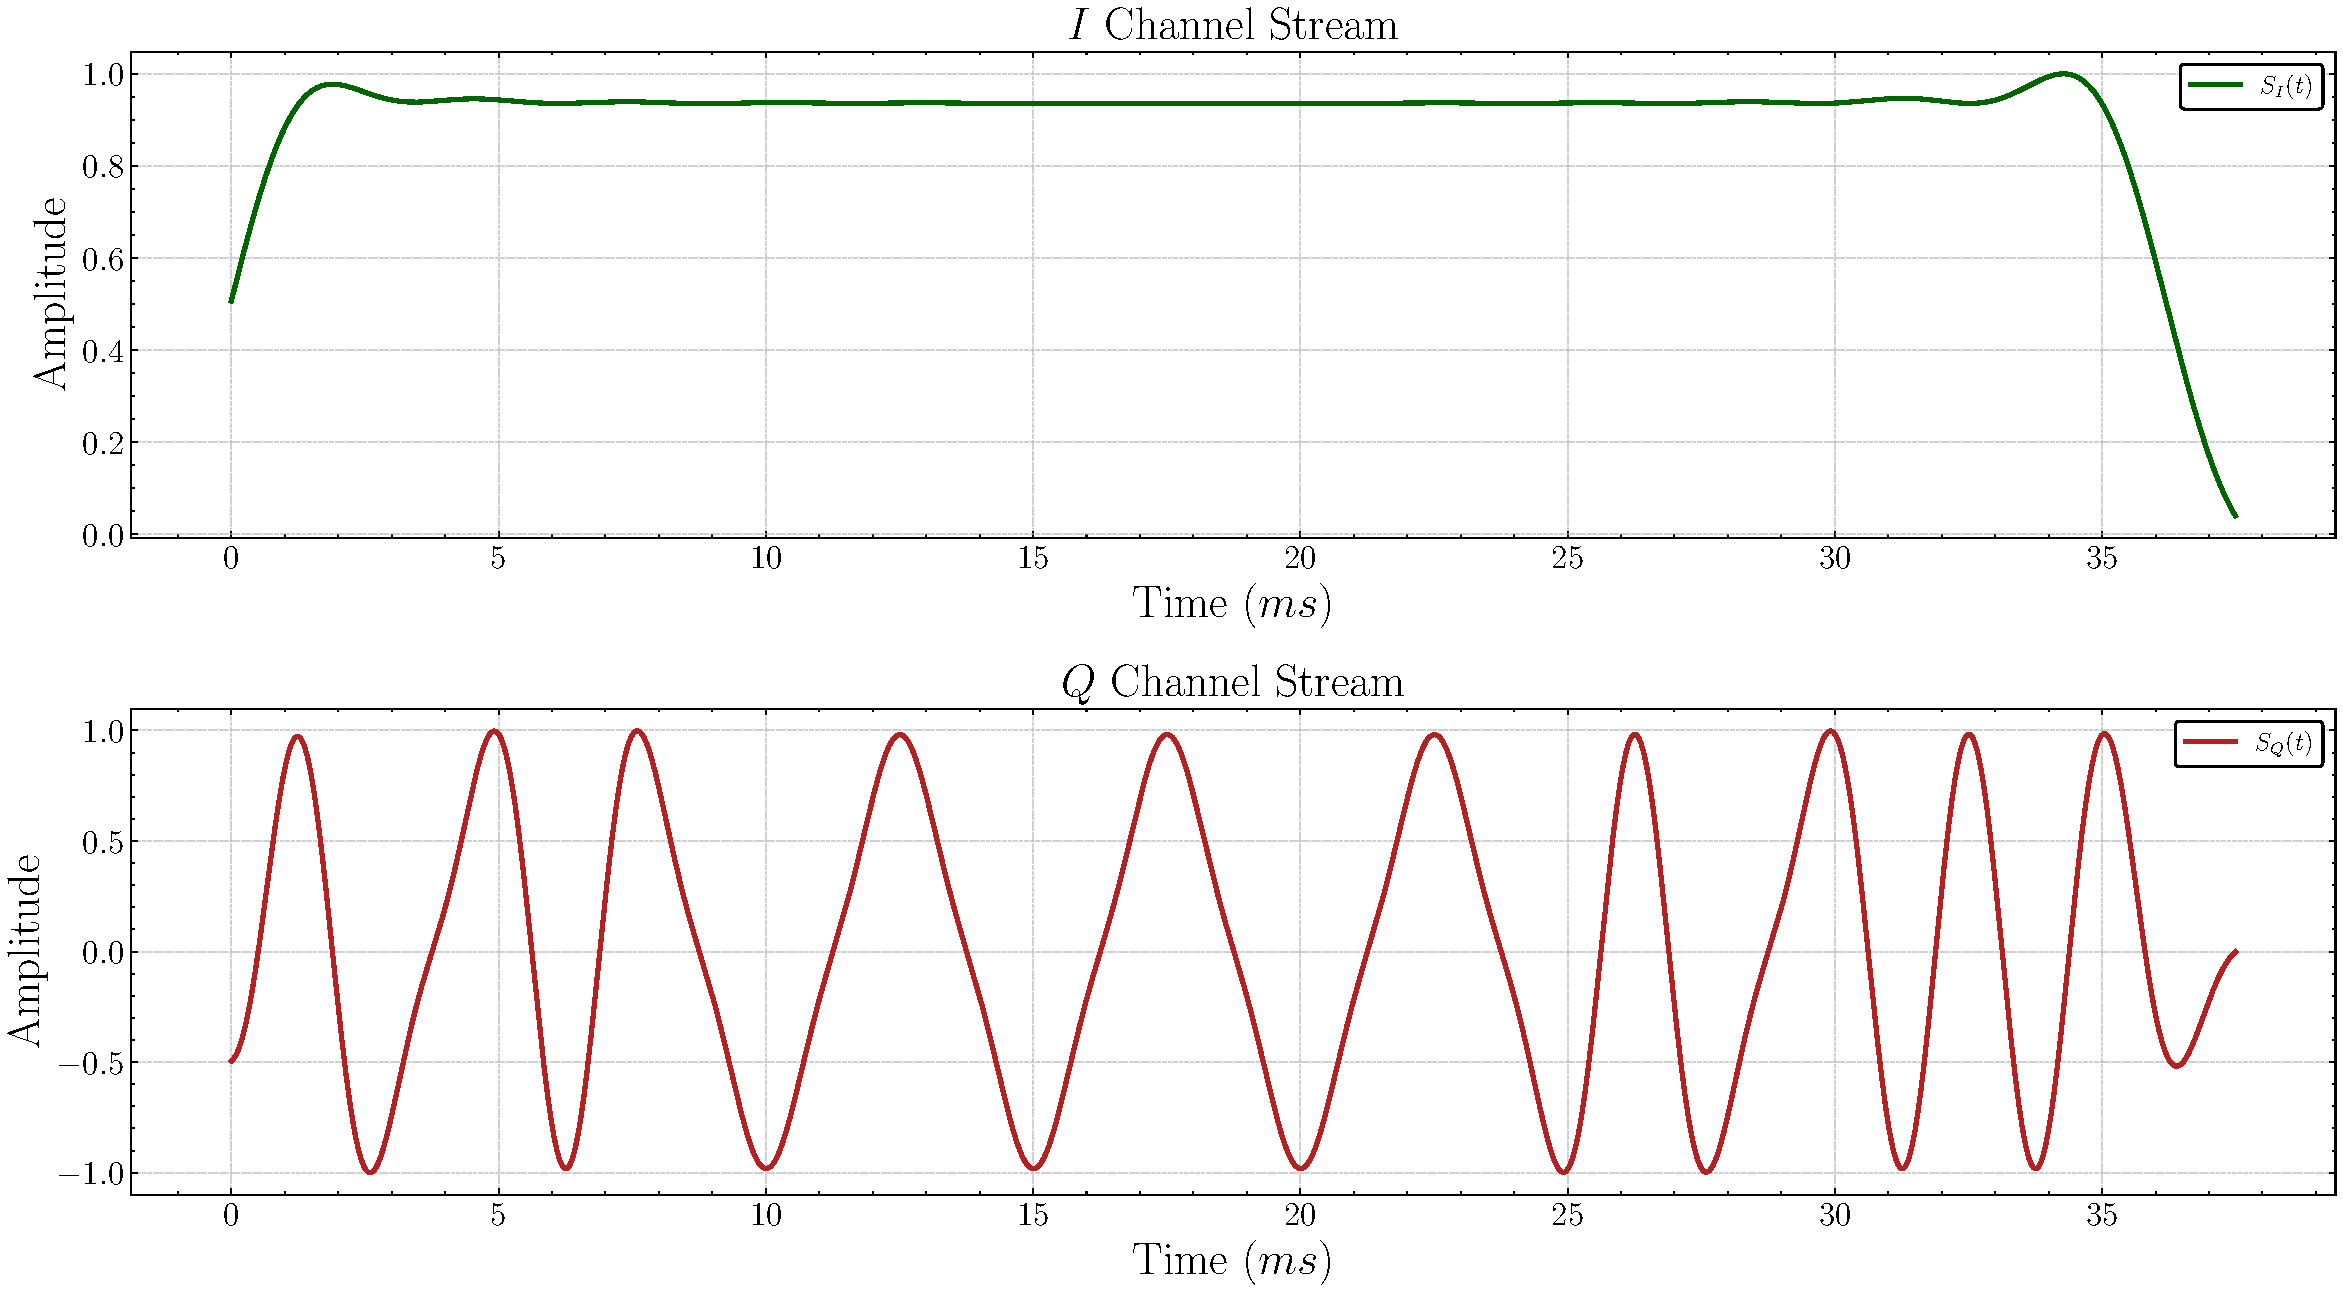
\includegraphics[width=\linewidth]{assets/cap3/example_synchronizer_word.pdf}
\end{figure}

\begin{figure}[H]
	\centering
	\caption{Módulo de correlação entre $I$ e $Q$ e vetor de sincronismo}\label{fig:receiver_corr}
	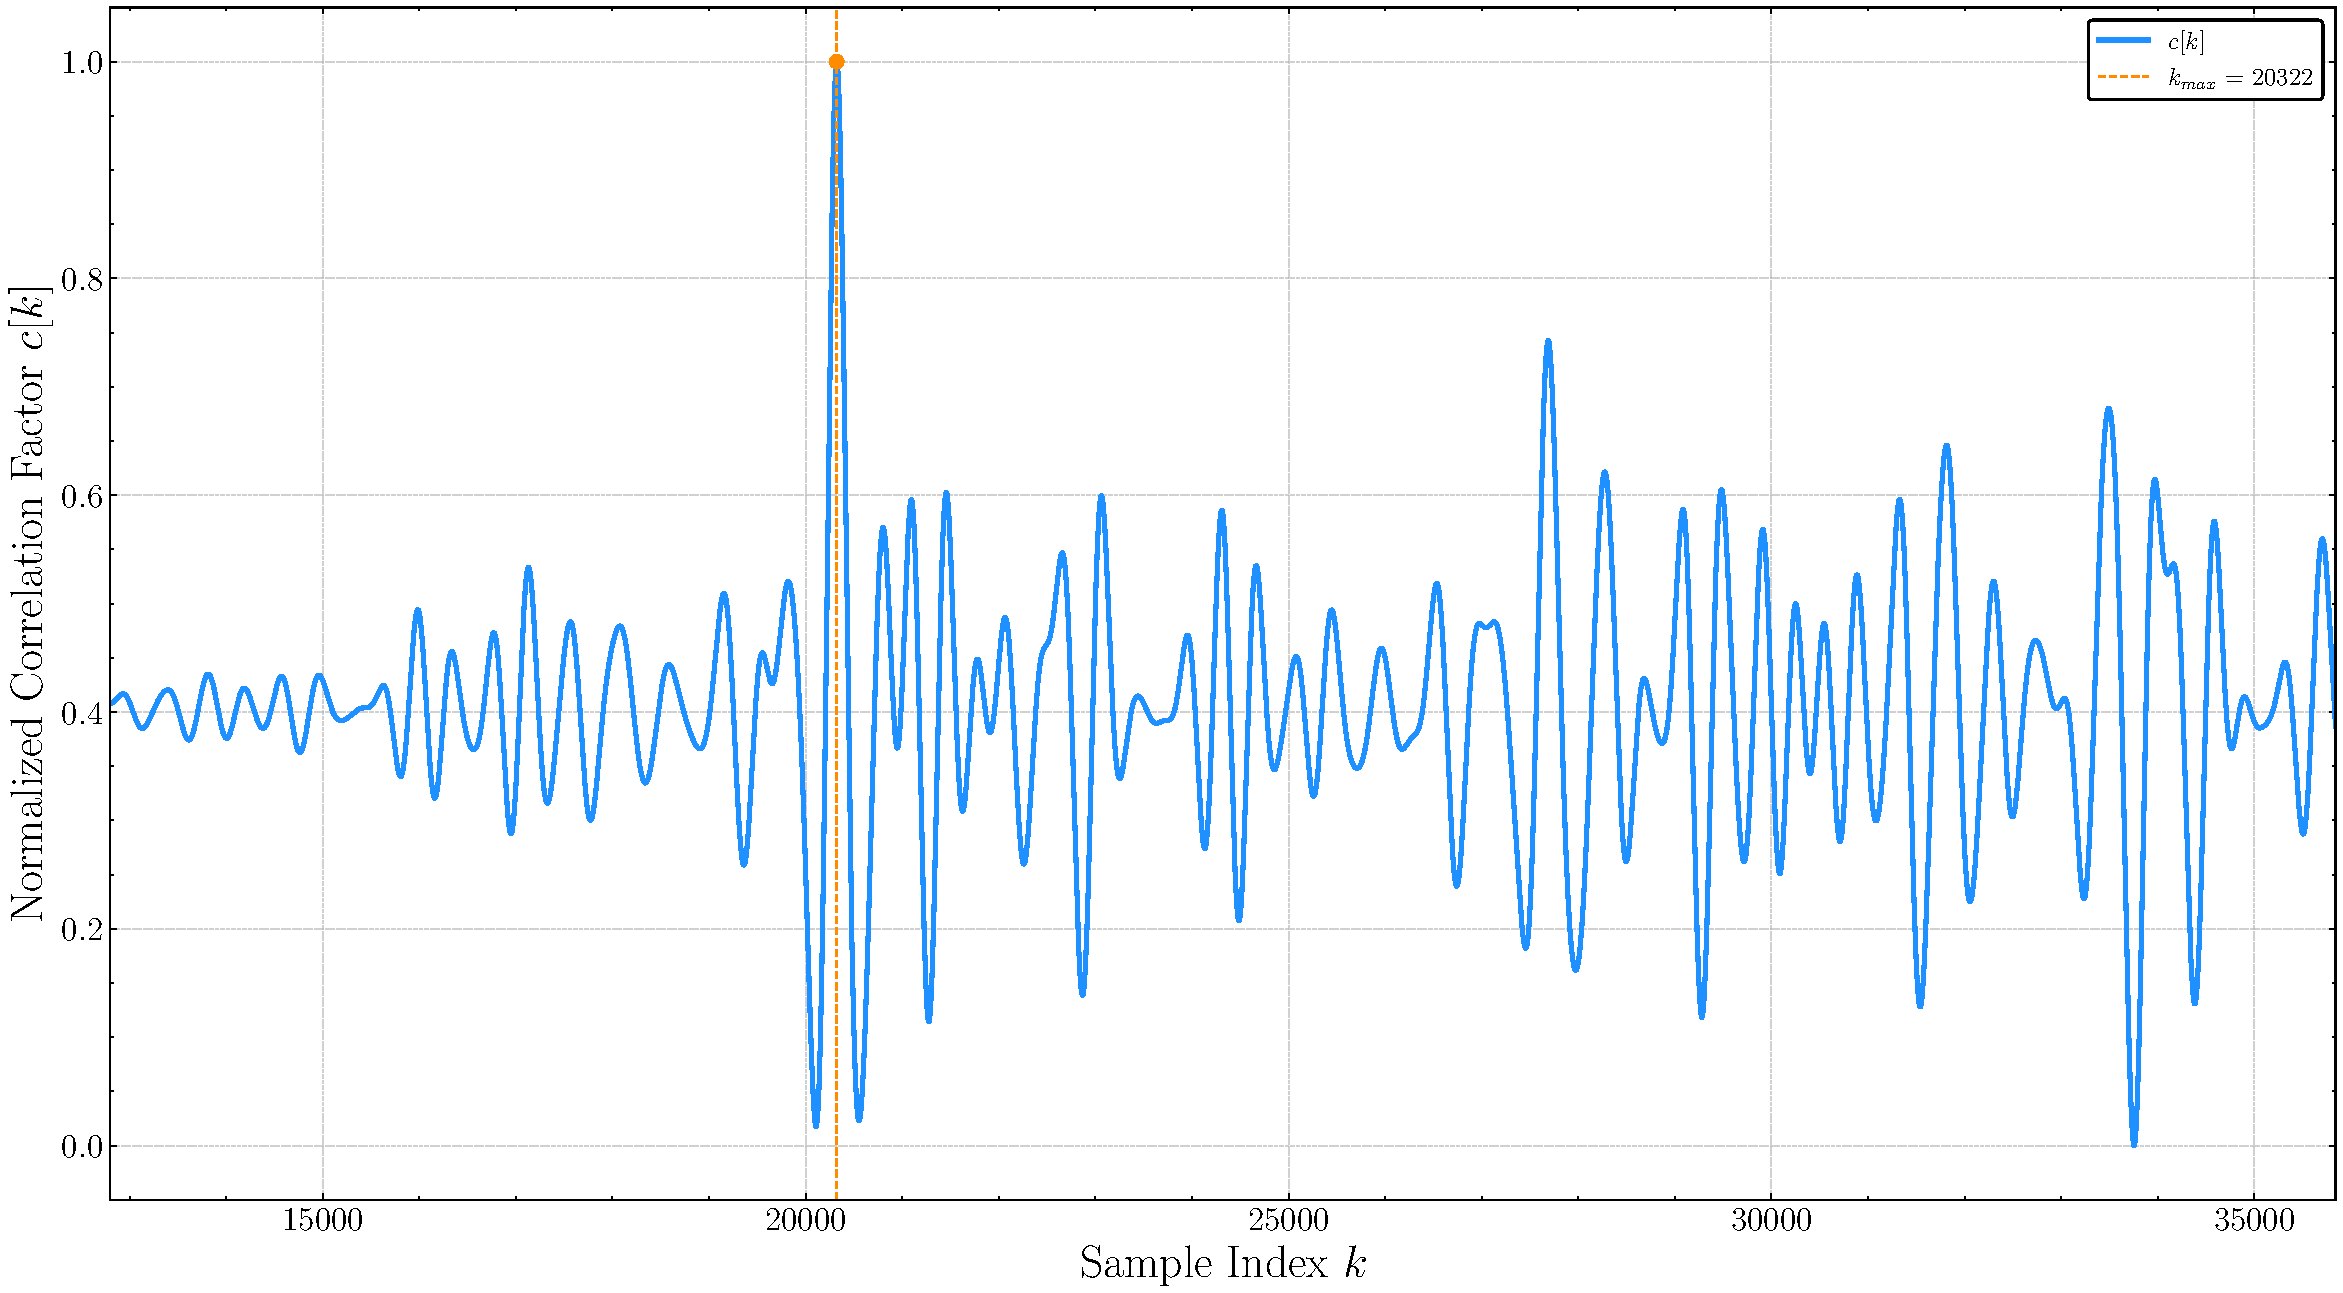
\includegraphics[width=\linewidth]{assets/cap3/receiver_sync_corr.pdf}
\end{figure}

\begin{figure}[H]
	\centering
	\caption{Sicronização de $I$ e $Q$ com vetor de sincronismo}\label{fig:receiver_sync}
	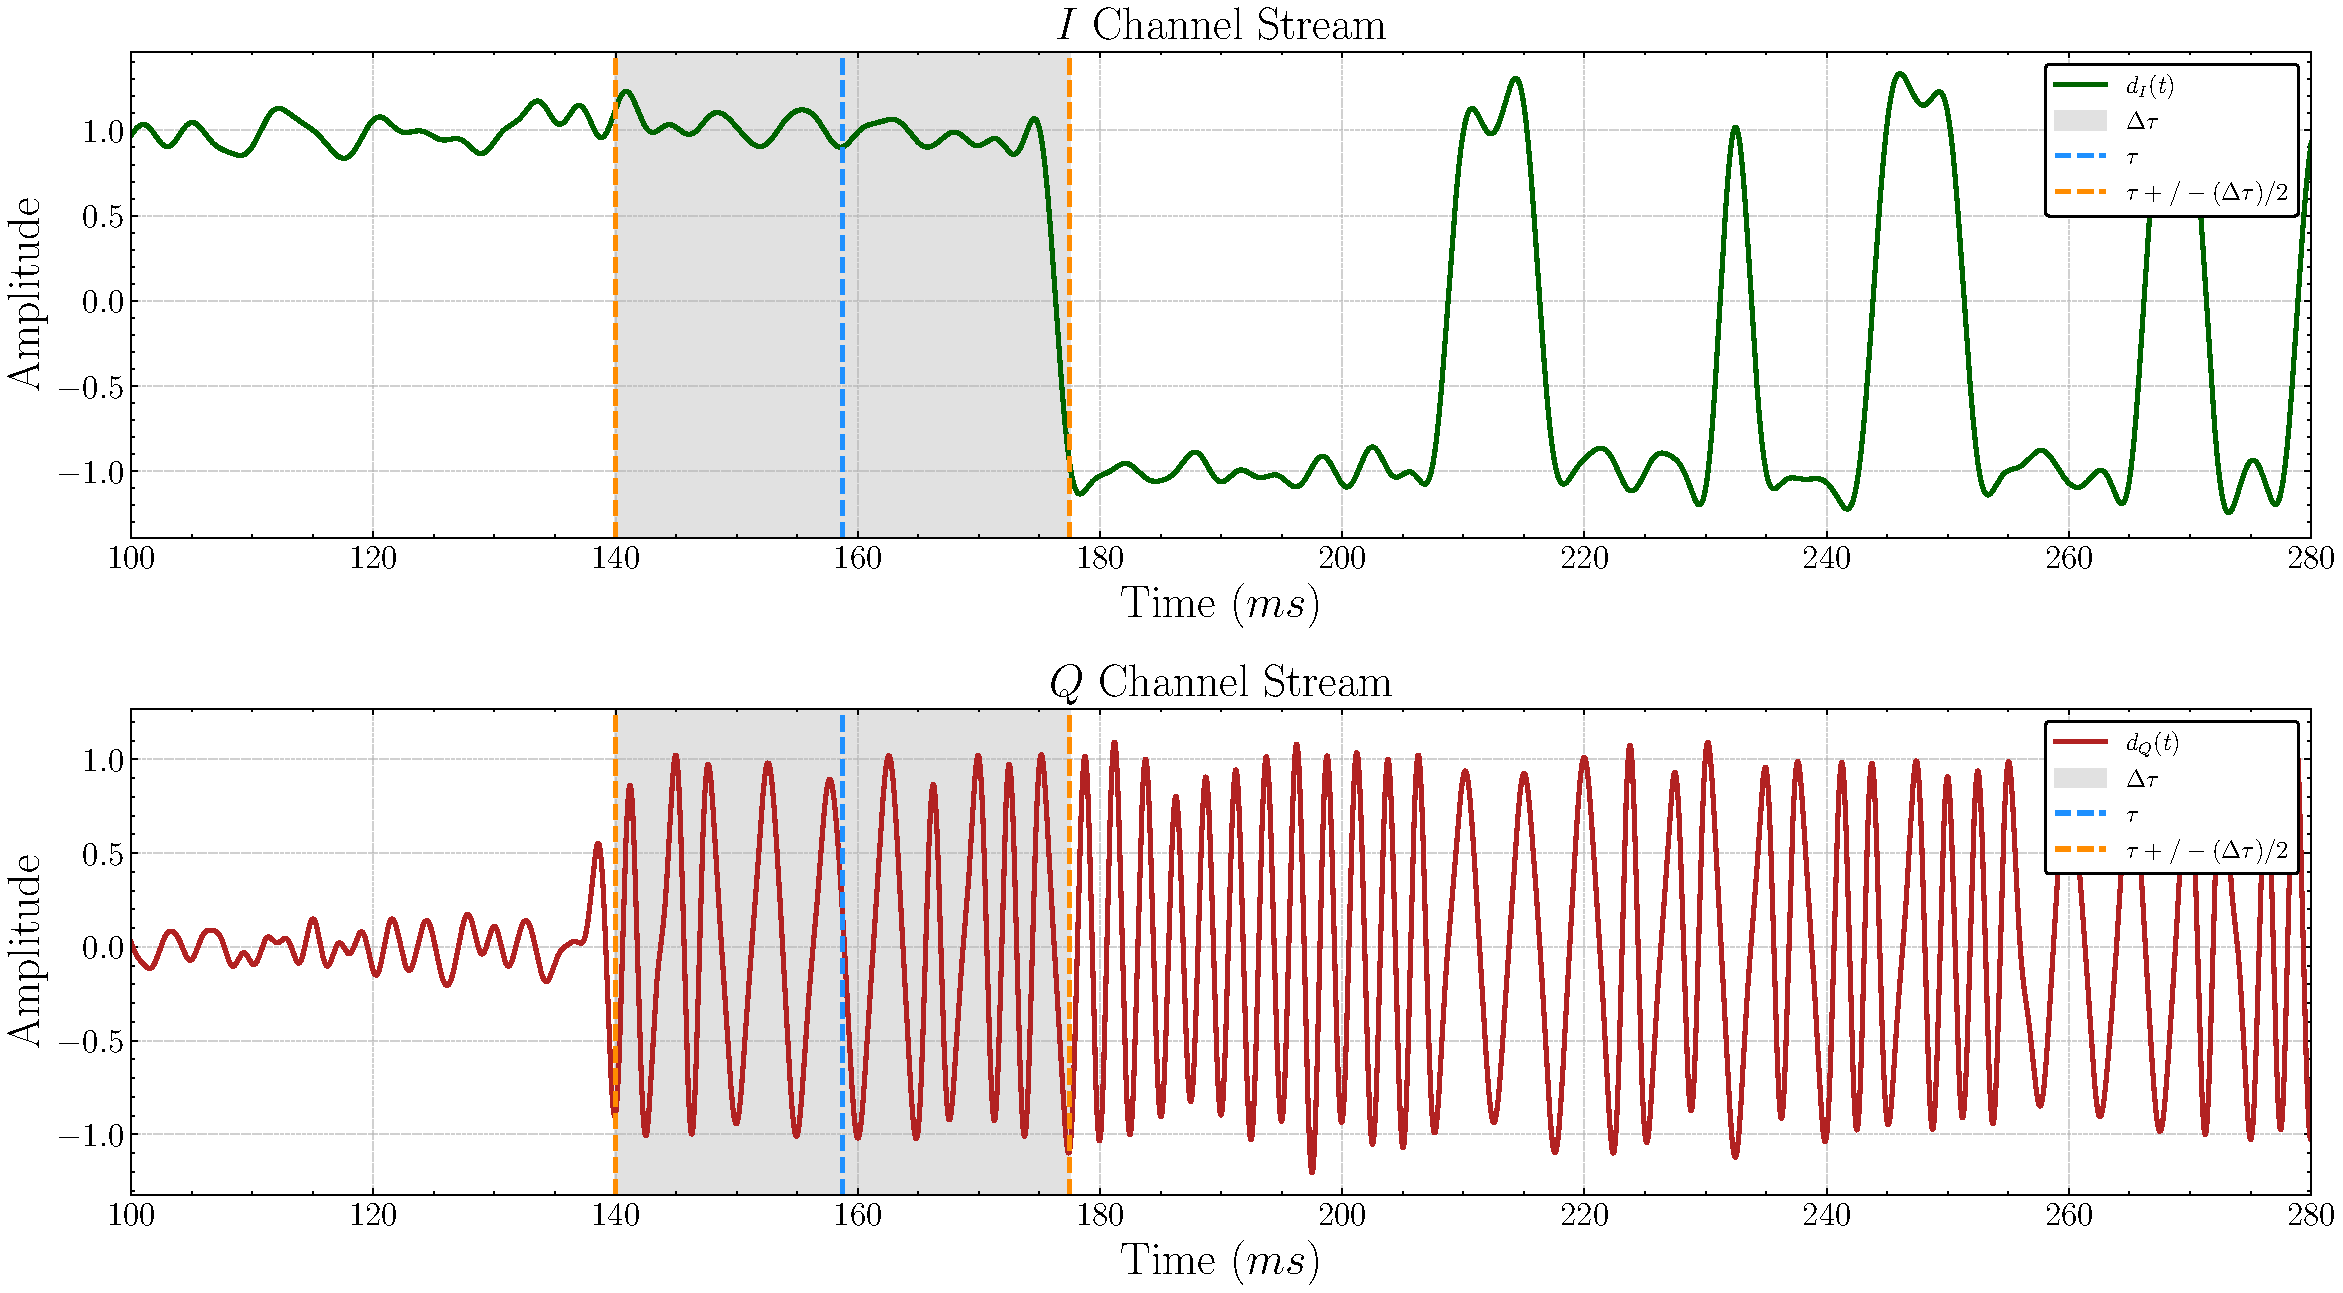
\includegraphics[width=\linewidth]{assets/cap3/receiver_sync_time.pdf}
\end{figure}


\subsection{Decisão de símbolos}\label{sec:decisao_simbolos}

\begin{figure}[H]
	\centering
	\caption{Amostragem dos canais $I$ e $Q$ em $T_b$ a partir de \gls{tau}}\label{fig:receiver_sampler}
	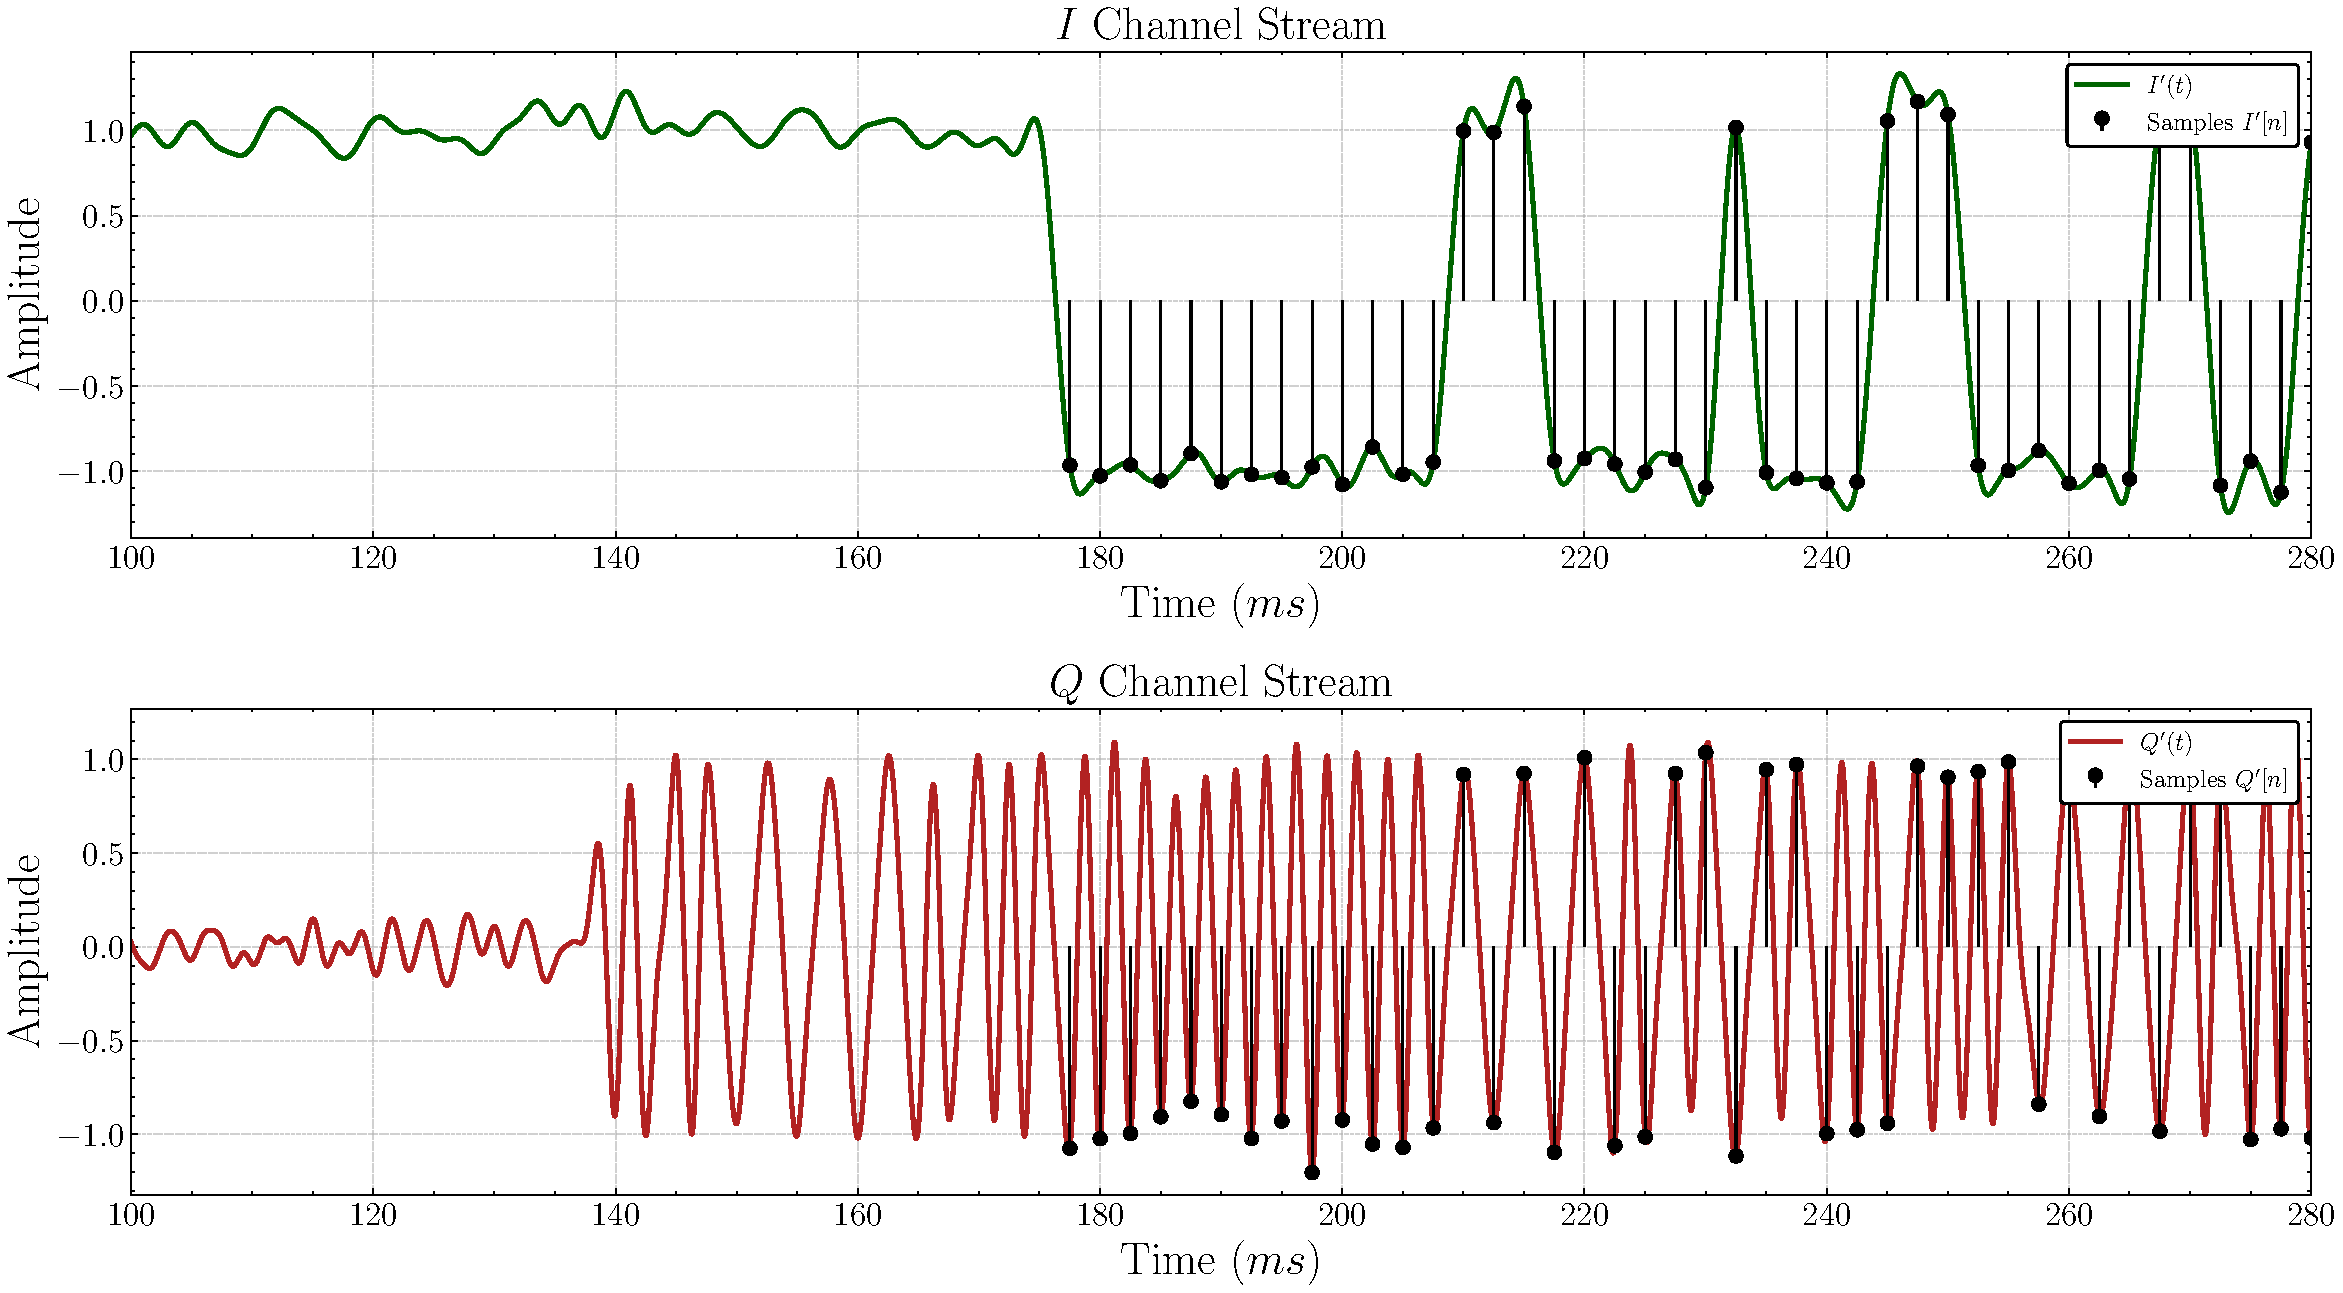
\includegraphics[width=\linewidth]{assets/cap3/receiver_sampler_time.pdf}
\end{figure}

\begin{figure}[H]
	\centering
	\caption{Constelação dos canais $I$ e $Q$ filtrados e amostrados}\label{fig:receiver_const}
	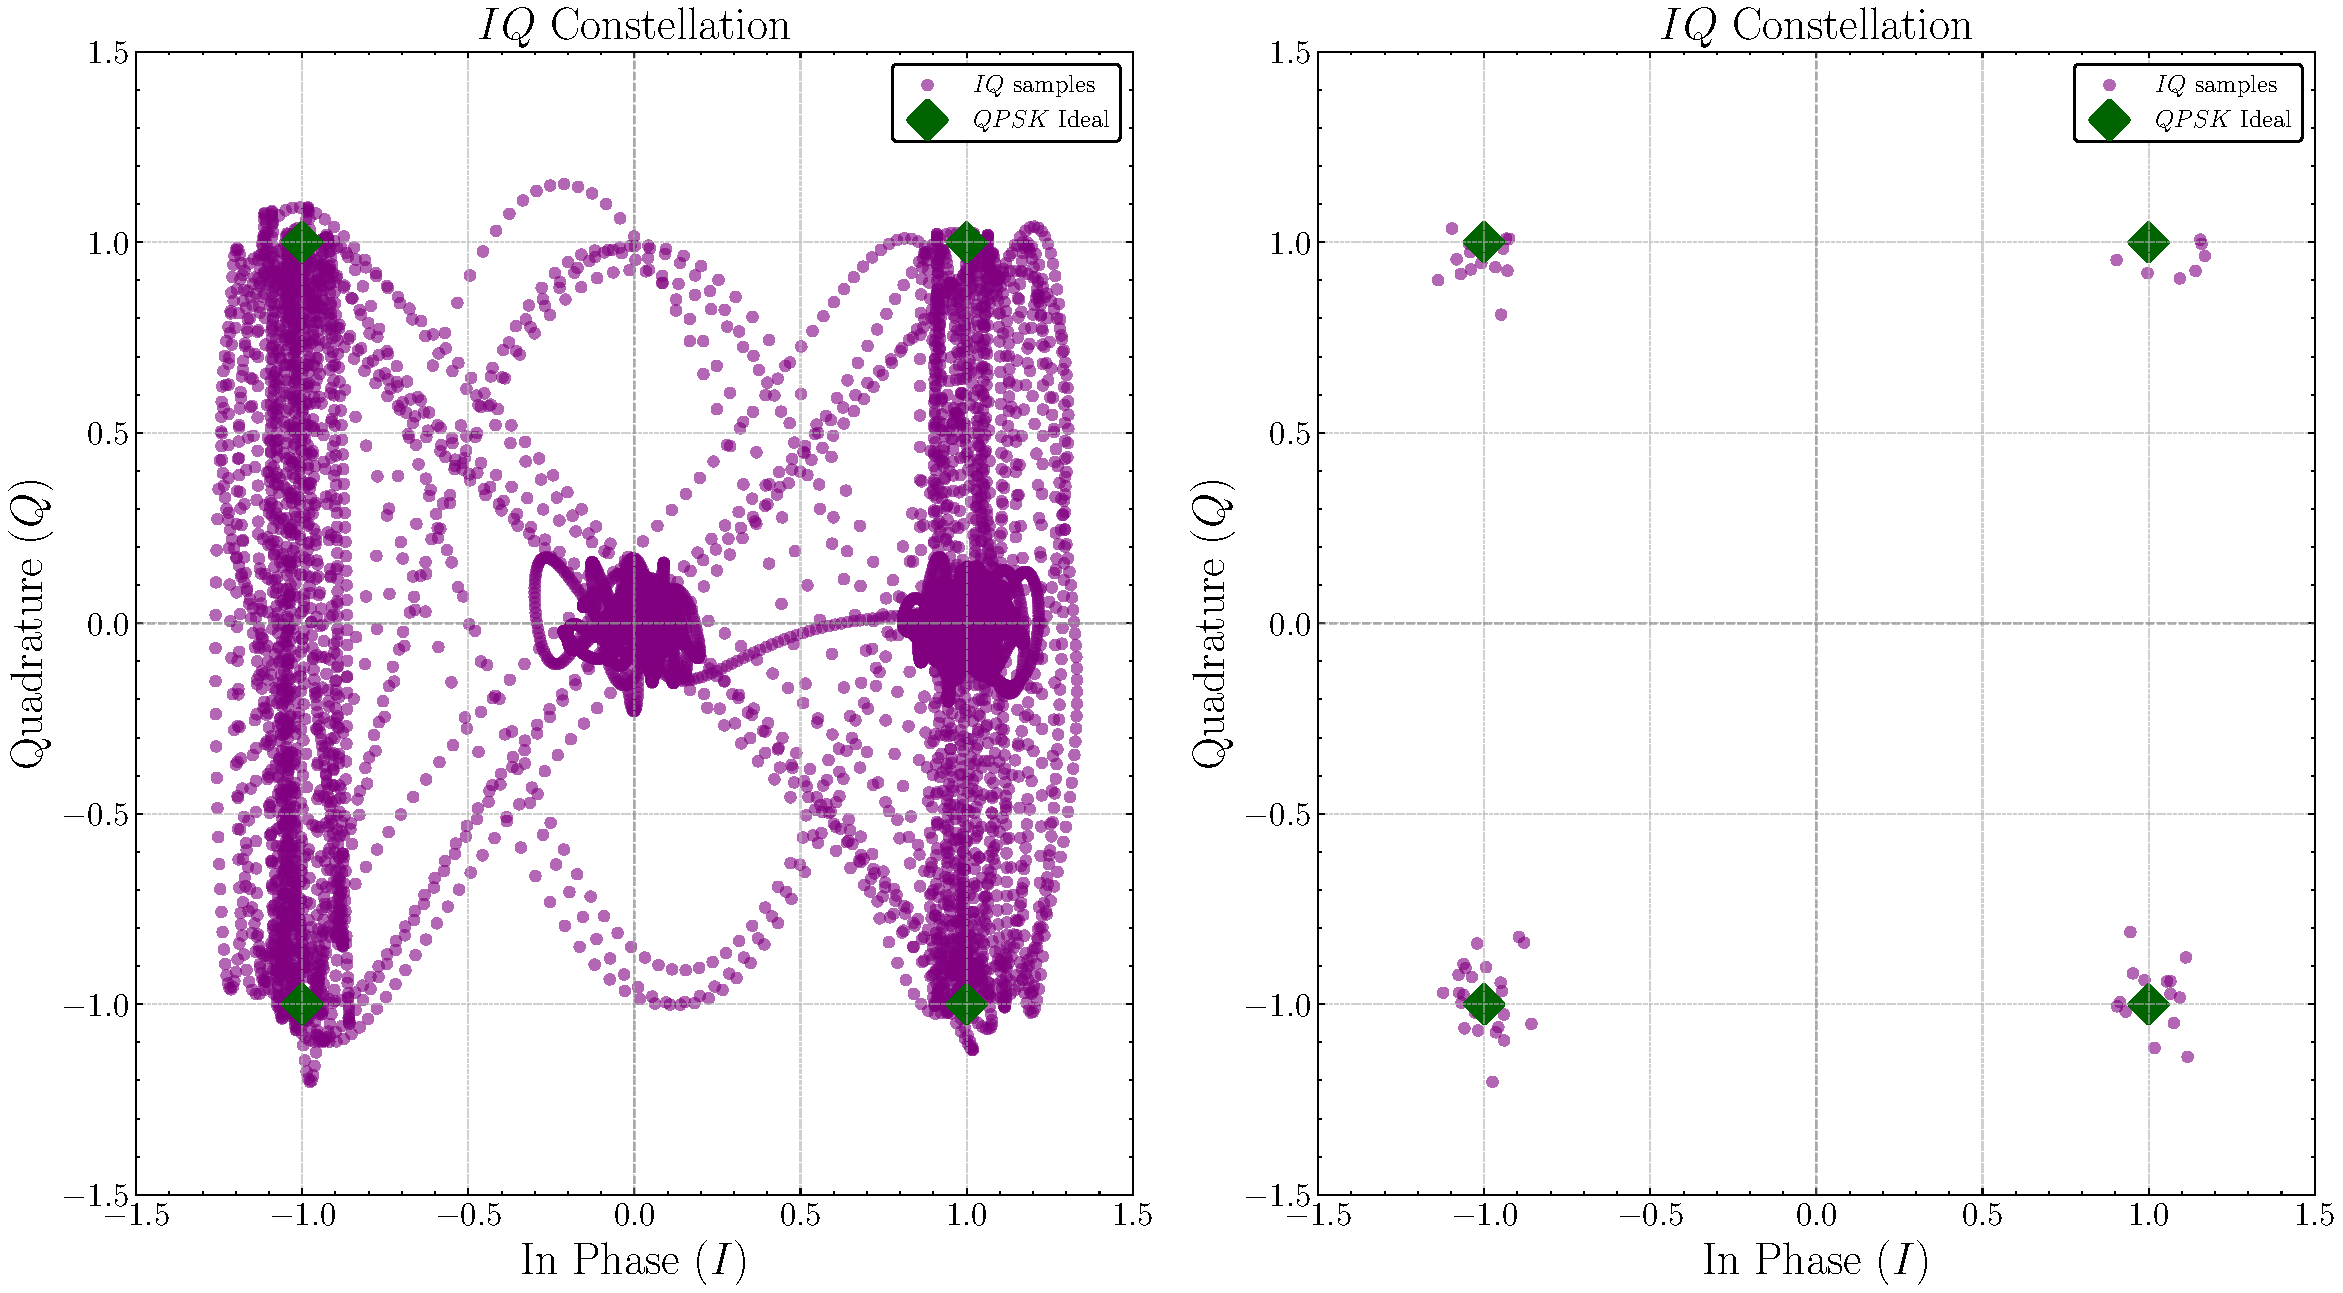
\includegraphics[width=\linewidth]{assets/cap3/receiver_sampler_const.pdf}
\end{figure}

\subsection{Recuperação do Datagrama}\label{sec:decodificacao_convolucional}

\begin{figure}[H]
	\centering
	\caption{Decodificação convolucional dos canais $I$ e $Q$}\label{fig:receiver_conv}
	\includegraphics[width=\linewidth]{assets/cap3/receiver_conv_time.pdf}
\end{figure}
\chapter{CONCLUSÃO}\label{cap:conclusao}

\subsection{Trabalhos futuros}

Com o desenvolvimento do projeto, alguns pontos que podem ser melhorados foram identificados: 
\begin{itemize}
    \item Aplicar técnicas de filtragem para a matriz de detecção, eliminando ruidos detectados e mantendo apenas as transmissões de interesse; 
    \item Alterar cadeia de recepção invertendo a ordem do decodificador convolucional para trabalhar com viterbi soft-decision;
    \item Aplicar modelagem de canal mais realista, adicionando desvio de frequência e efeito Doppler;
    \item Aplicar modelagem de canal mais realista, adicionando atenuação por distância e ACG (Automatic Gain Control);
    \item Realizar comparativo de desempenho da curva $BER \times E_b/N_0$ variândo parâmetros do sistema, como palavra de sincronismo, vetores geradores, tipo de codificação de linha, tipo de modulação de pulso, etc.
\end{itemize}



% Imprimir Referências
\printbibliography[title={Referências}]%

%-----------------------------------------------%
% Apêndices
%-----------------------------------------------%
\begin{apendicesenv}
\chapter{BER vs SNR}

Com base na implementação do receptor e transmissor apresentada nas seções \ref{sec:receptor} e \ref{sec:transmissor}, foi realizado um estudo de desempenho do sistema, variando a relação \gls{EbN0} e medindo a \gls{BER} para cada valor, comparando o desempenho do sistema ARGOS-3 com modulação \gls{QPSK} (tanto teórica quanto simulada), conforme apresentado na \autoref{fig:ber_snr}.

\begin{figure}[H]
	\centering
	\caption{Comparação BER vs SNR - ARGOS3 e QPSK}\label{fig:ber_snr}
	\includegraphics[width=\linewidth]{assets/apendice/ber_vs_ebn0.pdf}
\end{figure}

Nota-se que o desempenho do sistema ARGOS-3 está melhor do que o desempenho teórico e simulado da modulação \gls{QPSK} pura, o que pode ser explicado pela presença do código convolucional, que adiciona redundância aos dados transmitidos, permitindo a correção de erros no receptor, além da presença da técnica de codificação de linha \gls{Manchester}, que também contribui para a melhoria das características do sinal modulado.


\chapter{Simulador OpenSource ARGOS-3}

A implementação do transmissor e receptor ARGOS-3, conforme descrito nas seções \ref{sec:transmissor} e \ref{sec:receptor}, foi realizada em Python, utilizando bibliotecas open source como NumPy, SciPy e Matplotlib. O código-fonte completo do simulador está disponível no repositório GitHub \cite{githubrepository}, permitindo que outros alunos, professores e pesquisadores possam utilizar, modificar e contribuir para o desenvolvimento do projeto. A biblioteca ARGOS-3 utilizada na implementação pode ser instalada via `pip`, conforme mostrado no exemplo de instalação na \autoref{cod:argos3}. 

\lstinputlisting[language=bash,caption={Exemplo de instalação da biblioteca},label=cod:argos3]{codigo/install.sh}

O exemplo apresentado no \autoref{cod:argos3} demonstra o uso dos principais módulos da biblioteca, incluindo a criação de um transmissor, a transmissão de um datagrama, a detecção do canal e a recepção do datagrama.

\lstinputlisting[language=python,caption={Exemplo de uso dos principais módulos da biblioteca},label=cod:argos3]{codigo/argos3.py}

\end{apendicesenv}


\end{document}